\documentclass[a4paper]{report}

% !TEX root = .memoire/main.tex

\usepackage[utf8]{inputenc}
% \renewcommand{\familydefault}{\sfdefault}
\usepackage{geometry}
\usepackage[pdftex]{graphicx}

\graphicspath{ {./MeshlessEnKF}{./Introduction/images} {./MeshlessMethods/images} {./AlignEnKF/images} {./BiblioIntro/images} {./DataAssimilation/images}}
% \geometry{
%     left=16mm,
%     top=30mm,
%     right=16mm,
%     bottom=30mm
% }
\usepackage{appendix}
\usepackage{etoolbox}
\usepackage{xcolor}
\usepackage[absolute,overlay]{textpos}
\usepackage{lipsum}
\usepackage{array}
\usepackage{enumitem}
\usepackage{caption}
\usepackage{multicol}
\usepackage{bm}
\usepackage{amsmath}
\usepackage{amsfonts}
\usepackage{subcaption}
\usepackage[vlined, french, onelanguage]{algorithm2e}
% Hyperref setup
\usepackage[linktoc=page]{hyperref}
% \hypersetup{
%     colorlinks=true,
%     linkcolor=blue,
%     filecolor=magenta,
%     urlcolor=cyan,
%     pdftitle={Overleaf Example},
%     pdfpagemode=FullScreen,
% }
\hypersetup{
    % General settings
    pdfencoding=auto,           % Automatically handles PDF string encoding
    pdfborder={0 0 0},          % Removes borders around links
    breaklinks=true,            % Allows links to break across lines
    colorlinks=true,            % Colors the text of links and anchors
    % Link colors
    linkcolor=blue,             % Color of internal links (e.g., sections, equations)
    citecolor=green,            % Color of citation links
    filecolor=magenta,          % Color of file links
    urlcolor=cyan,              % Color of external hyperlinks
    % Metadata
    pdftitle={thesis duvillard},       % Title of the document
    pdfauthor={duvillard},              % Author of the document
    % pdfsubject={thesis},          % Subject of the document
    % pdfkeywords={keyword1, keyword2},   % Keywords for the document
    % PDF display settings
    pdfpagemode=UseOutlines,    % Opens the PDF with the bookmarks pane open
    bookmarksopen=true,         % Open the bookmarks by default
    bookmarksnumbered=true,     % Include section numbers in bookmarks
    unicode=true                % Support for non-ASCII characters in bookmarks
}
\urlstyle{same}
\setlength{\columnseprule}{0pt}
\setlength\columnsep{10pt}
\usepackage[most]{tcolorbox}
\usepackage{amsthm}
\theoremstyle{definition}
\newtheorem{definition}{Definition}%[section]

\definecolor{mycustomcolor}{RGB}{128, 0, 128}
\newcommand{\mycolor}[1]{\textcolor{mycustomcolor}{#1}}
\newcommand{\bE}{\mathbb{E}}
\newcommand{\bV}{\mathbb{V}}
\newcommand{\bC}{\mathbb{C}}
\newcommand{\nens}{N}
\newcommand{\bw}{\bm w}
\DeclareMathOperator*{\argmax}{arg\,max}
\DeclareMathOperator*{\argmin}{arg\,min}
\newcommand{\bx}{\bm{x}}
\newcommand{\mstate}{\bm{Z}}
\newcommand{\statebis}{\bm{x}}
\newcommand{\mstatebis}{\bm{X}}
\newcommand{\zz}{z_0 = 0.02}
\newcommand{\sigz}{\sigma_0^2 = 0.5}
\newcommand{\xx}{x_0 = 0.02}
\newcommand{\sigx}{\sigma_0^2 = 0.5}
\newcommand{\npart}{$N_{part} = 100$}
\newcommand{\ngrid}{$N_{grid} = 100$}
\newcommand{\sigmaY}{0.05}
\newcommand{\z}{\bm{z}}

\newcommand{\mpred}{\mathcal{Y}}
\newcommand{\mP}{\mathcal{P}}
\newcommand{\Fcorr}{\bm{F}}
\newcommand{\mdata}{\bm{D}}
\newcommand{\state}{\bm{z}}
\newcommand{\annomX}{\bm A}
\newcommand{\annomY}{\bm Y}
\newcommand{\obs}{\bm{y}}
\newcommand{\Cov}{\bm{P}}
\newcommand{\predi}{\mathcal{H} (\bm{x}_i^f)}
\newcommand{\sigmaZm}{0.5}
\newcommand{\meanZm}{\pi/2 + 0.6}
\newcommand{\bz}{\bm z}
\newcommand{\visc}{D}
\newcommand{\refv}{1.0}
\newcommand{\refvisc}{0.05}
\newcommand{\Dlow}{0.02}
\newcommand{\Dup}{0.08}
\newcommand{\vmean}{0.9}
\newcommand{\vstd}{1.2}
\newcommand{\smLow}{0.8}
\newcommand{\smUp}{1.2}

\newcommand{\by}{\bm{y}}
\newcommand{\bP}{\bm{P}}
\newcommand{\bR}{\bm{R}}
\newcommand{\bh}{\bm{h}}
\newcommand{\bd}{\bm{d}}
\newcommand{\fstate}{\bm{u}}
\newcommand{\cN}{\mathcal N}
\newcommand{\cU}{\mathcal U}
\newcommand{\cP}{\mathcal P}
\newcommand{\cV}{\mathcal V}

\newcommand{\bM}{\bm{M}}
\newcommand{\bH}{\bm{H}}
\newcommand{\bK}{\bm{K}}

\DeclareMathOperator{\Tr}{Tr}
\usepackage[most]{tcolorbox}

% Définition du modèle "boite1"
\newtcolorbox{ObjectifChap}[1][]{
    colback=blue!5!white,
    colframe=blue!75!black,
    fonttitle=\bfseries,
    title=Boîte 1,
    #1
}

% Définition du modèle "boite2"
\newtcolorbox[auto counter]{BilanChap}[1][]{
    colback=red!5!white,
    colframe=red!75!black,
    fonttitle=\bfseries,
    title=Boîte \thetcbcounter,
    #1
}
\newcommand{\norm}[1]{\left\lVert #1 \right\rVert}

\usepackage[french]{babel}
\usepackage{biblatex}
\addbibresource{biblio.bib}
% \bibliographystyle{plain}


\title{
{Méthodes d'assimilation de données pour des simulations lagrangiennes}\\
{\large Ecole Polytechnique / CEA Cadarache}
}
\author{Marius Duvillard}
\date{\today}

\begin{document}

\maketitle
\tableofcontents

\chapter{Introduction}

Dans le domaine de la production d'énergie electrique, l'énergie nucléaire est une source d'énergie qui s'est imposé à de nombreux pays industrialisés.

En 2023, l'industrie électronucléaire a représenté 65\% de la production totale d'électricité en France, avec un parc composé de 56 réacteurs à eau pressurisée (REP) répartis sur 18 centrales \cite{rte2023}. Dans le monde, la production nucléaire ne fait qu'augmenter. Fin 2022, la capacité totale des 438 réacteurs nucléaires de puissance en exploitation dans 32 pays s’établissait à 393,8 gigawatts électriques (GWe). Si aujourd'hui, le nucléaire représente près de 9,8\% de la production mondiale, elle pourrait attendre 14\% du bouquet électrique en 2025 \cite{aiea2023}. D'ici 2035, le nombre de pays qui exploitent des centrales nucléaires pourrait augmenter de quelque 30\% d'ici 2050.

Le secteur est également en constante mutation avec le développement de nouvelles technologies en particulier avec les technologies de 4\textsubscript{ème} génération mais également le nouveau paradigme des SMR (\textit{Small Modular Reactor}) où la modularité permet une chaîne de déploiment et de production souple et avec une financement moindre~\cite{academie2022}.

Si ce secteur atire, c'est en particulier car il offre un très bon rapport qualité prix et est faiblement émettrice en gaz à effet de serre. Son facteur d'émission, c'est à dire la quantité d'émissions de gaz à effet de serre par unité d'énergie produite, est estimé à 12 g$CO2$eq/kWh. Il serait même encore plus faible en France~\cite{schlomer_technology-specific_nodate}. Ainsi elle est aussi émetrice que l'éolien ou bien la production photovoltaïque et est 100 à 1000 fois moins émettrice que les centrale à énergie fossiels.

L'urgence climatique pousse à considérer l'énergie nucléaire comme un levier essentiel dans la transition énergétique, offrant une alternative viable aux énergies fossiles. Cependant, cette option soulève une série de préoccupations. Outre les inquiétudes liées à la sécurité des installations et au risque de prolifération nucléaire~\cite{npt_resolution}, il est crucial d'aborder la question des déchets hautement radioactifs générés tout au long du fonctionnement des réacteurs. Chaque année, la production d'électricité entraîne la création de près de 2 kg de déchets par habitant. Une infime proportion constitue les déchets à vie longue, mais ils représentent la majorité de l'activité radioactive (0.2\% des stocks pour 95\% de l'activité). En outre, il est impératif de préserver les réserves de combustible nucléaire. Dans cette optique, les avancées technologiques telles que les réacteurs de quatrième génération visent à optimiser l'utilisation des ressources en transmutant l'uranium 238 en plutonium 239. Ainsi, la question du retraitement et de la fermeture du cycle nucléaire reste cruciale. C'est dans cette perspective que le combustible MOX (Mélange d’OXyde de plutonium et d’OXyde d’uranium) a été développé afin de recycler une partie des matières nucléaires issues du traitement des combustibles à Uranium Naturel Enrichi (UNE).

La fabrication de ce combustible passe par différentes étapes de fabrication en particulier une phase de mélange et de broyage qui a lieu au sein d'un broyeur à boulets. Ce dispositif cylindrique, rempli de boules de broyage, met en oeuvre un processus de rotation pour broyer finement le mélange de poudres d'oxyde. Sa performance est critique pour la qualité du produit final et sa sûreté d'utilisation dans les réacteurs nucléaires. Cependant, son contrôle est déterminé de manière empirique par l'expérimentateur sur une variété de paramètres tel que la vitesse de rotation, le degré de remplissage, les proportions d'alimentation et de corps broyants. Le large spectre des physiques mise en jeu à l'intérieur du tambour mais aussi le contexte de manipulation de poudres irradié rendent le contrôle et l'optimisation très complexe. Ceci a pour conséquence d’augmenter le temps de broyage, la consommation du procédé et le nombre d’intervention nécessaire sur l’installation.

C'est dans ce contexte que des outils d'aide à la compréhension par la modélisation et la simulation des étapes de la fabrication du combustible sont développées. L'objectif étant de pouvoir faire le suivi de l'état du milieu granulaire sur une large gamme de paramètre ainsi que de comprendre les mécanismes intervenant dans ce processus.

En particulier, le CEA a développé des outils pour la simulation l'état du mélange dans le milieu granulaire à l'aide de méthodes sans maillage afin de représenter.

Le problème est que ces modèles reposent toujours sur des hypothèses simplificatrices limitant leurs champs d'action. De plus, les modèles dépendent de paramètres qu'il est nécessaire de calibrer. Enfin, l'incertitude de modélisation qui en découle a pour conséquence d'augmenter l'erreur de prédiction de modèle.

Par données expérimentales nous entendons toutes données qui peut être fournies par le dispositif expérimental.

C'est ce qui justifie cette thèse, elle consiste à développer des méthodes capables de combiner les données issue de la simulation et des données exéprimentales au sein du développement du Jumeau Numérique du procédé. Le jumeau numérique est une réplique virtuelle d'un système physique, permettant de simuler, d'analyser et de prédire le comportement du système physique en temps réel. Ce modèle numérique intègre des données dynamiques et historiques, permettant une représentation précise et **synchronisée** dans le temps. Dans le contexte industriel, les jumeaux numériques utilisent l'**intelligence artificielle** (IA), l'analyse de données, et les capteurs physiques pour améliorer la compréhension des processus et faciliter la prise de décisions.


C'est dans ce contexte de la fabrication du combustible MOX (pour Mélange d’OXyde de plutonium et d’OXyde d’uranium)


\section*{Objectifs de la thèse}
% Plan de la démarche comme évoqué dans la formation.
% !TEX root = memoire/main.tex

\chapter{Contexte}

\section{Introduction}

L'objectif de ce chapitre est de présenter les différentes entitées nécessaires à la construction d'un jumeau numérique. Nous présenterons tout d'abord, quels sont les modélisations physiques utlisés pour simuler l'étape du broyeur à boulets. Nous traiterons uniquement la modélisation du mélange et de l'écoulement granulaire au sein du tambour en rotation. Dans un second temps, nous présenterons les méthodes d'acquision utilisé pour . Finalement, nous présenterons la notion de jumeau numérique et présenterons dans quel cadre observation et simulation peuvent-ils être mis en relation.

\section{Simulation de l'écoulement granulaire au sein du broyeur à boulets}~\label{sec:simu_broyeur}

\subsection{Ecoulement d'un milieu granulaire}~\label{sec:simu_granulaire}

La simulation du broyeur repose sur la représentation de l'écoulement d'un milieu granulaire. Si les écoulements granulaires sont très présents dans la nature et dans l'industrie, du fait de la nature discrète du milieu, ils sont bien moins comprise que l'écoulement d'un liquide qui se base sur les équations de Navier-Stokes.

L'écoulement granulaire va se distinguer par trois types de régime que l'on assimile généralement aux trois états de la matière: solide où où le mouvement des particules est lent et le comportement est presque statique, une couche semblable à un liquide dans laquelle les grains s'écoulent avec une certaine inertie, et une zone semblable à un gaz où les particules se déplacent à des vitesses plus élevées de manière chaotique. Ils interviennents simultanément dans l'écoulement. Ce qui complexifie sa caractérisation rhéologique.

\begin{figure}
    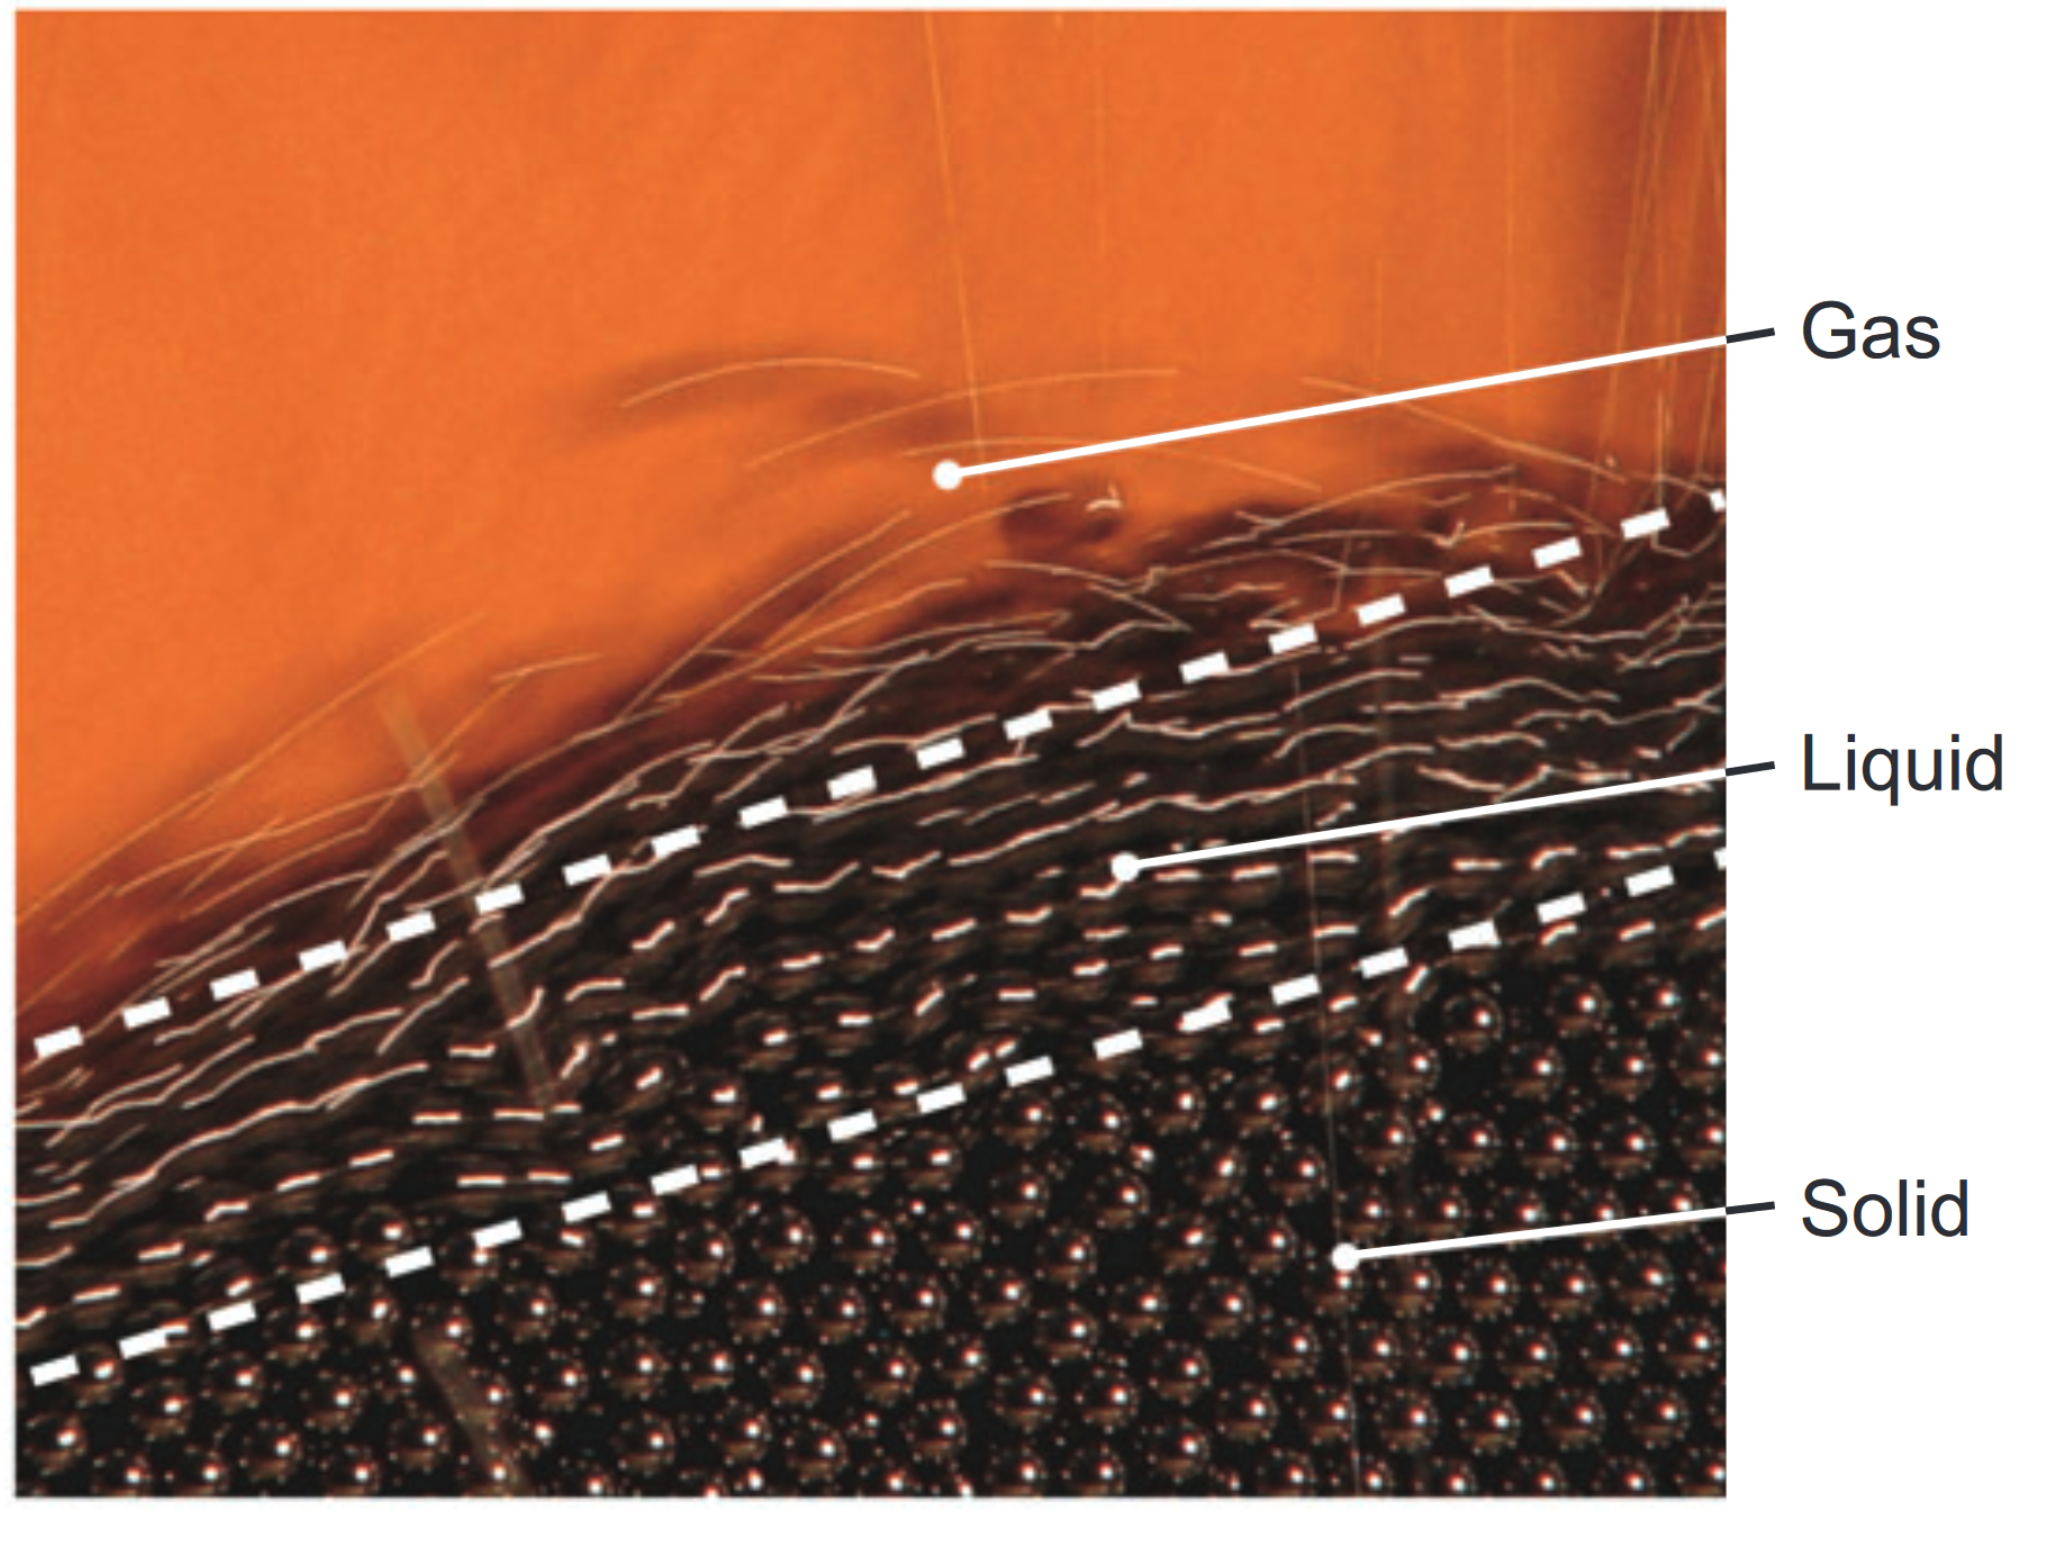
\includegraphics[width=\textwidth]{three_regimes.png}
    \caption{Image de billes d'acier s'écoulant d'un tas. Trois phases de l'écoulement granulaire, se comportant comme un gaz, un liquide ou un solide, peuvent être identifiées.~\cite{forterre_flows_2008}}
\end{figure}

Le régime solide ou frictionnel intervient en particulier en mécanique des sols pour la prédiction de la défaillance des sols pour les applications de génie civil~\cite{Campbell2006}. Dans ce cas, le critère de rupture de Mohr-Coulomb~\cite{Juvinal1991}, accompagné d'une règle de flux de la plasticité des métaux, est suffisant pour décrire le comportement de l'écoulement granulaire comme un processus continu, sans prendre en compte l'interaction des grains individuels. La loi est alors paramétré par des quantités interprétables : l'angle de friction interne, la cohésion, ainsi que l'angle de dilatation. La loi de Drucker-Prager~\cite{Drucker1952}, version lisée du critère de Mohr-Coulomb est également couremment utilisée.


Le régime liquide ou d'écoulement est principalement décrit à l'aide de lois rhéologique. Les travaux récents convergent vers une loi de comportement viscoplastique défini sous le nom de loi $\mu(I)$~\cite{gdr_midi_dense_2004,jop_constitutive_2006}. Des simulation du tambour en rotation~\cite{Cortet_2009} ont pu êter réalisé et montre une bonne correspondance pour le cas d'écoulement avec surface libre~\cite{chou_cross-sectional_2009}. Toutefois, cette loi trouve certaines limites dans le cas d'écoulement confiné où le coefficient de tassement change et où le mouvement de chaque grain entraîne des modifications significatives dans les chaînes de force. Si la prédiction est bonne au niveau des bords, elle reste toutefois insufisante au niveau des parois~\cite{Rognon_Miller_Metzger_Einav_2015}.

Finalement le régime gaz ou cinétique correspond au écoulement granulaires dispersés. Ce sont alors des modèles de cinétique des gaz qui sont utilisé pour modéliser le comportement du milieu granulaire~\cite{Ng2008}.

\subsection{Méthodes de résolution}~\label{sec:methode_resolution}

Dans le tambour en rotation l'ensemble des trois zones d'écoulement sont présentes. En fonction du nombre de Foudre, divers régimes d'écoulement apparaissent~\cite{MELLMANN2001251}. Entre autres, on retrouve le glissement, l'avalanche, la cascade, le cataracte, la centrifugation illustrés Figure~\ref{}

\begin{figure}~\label{fig:flow_drum}
    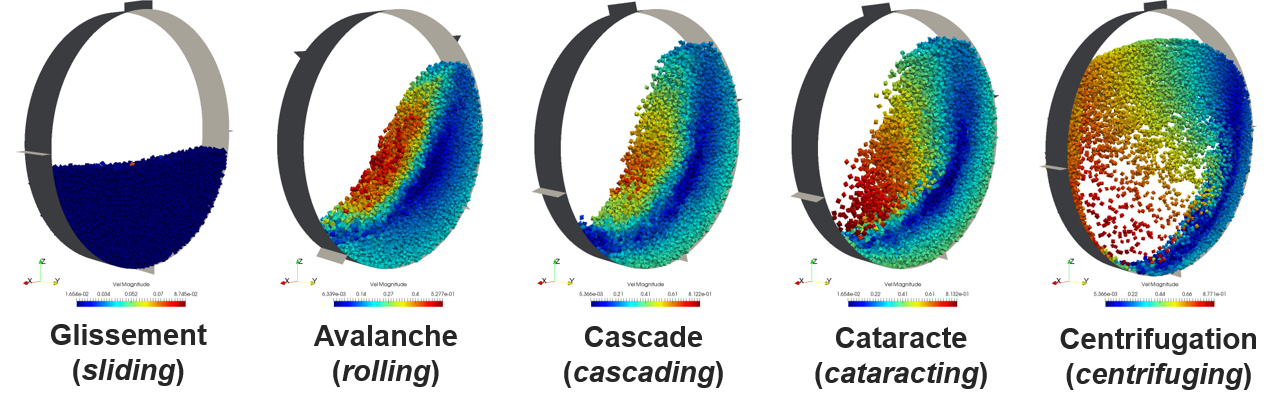
\includegraphics[width=\textwidth]{flows_in_drum.png}
    \caption{Représentation des différents régimes d'écoulement au sein du tambour en rotation avec la méthode DEM.}
\end{figure}

Ces différents régimes déterminent la qualité du mélange, du broyage. C'est en particulier le régime en cascade qui est recherché pour la réduction de taille de grain dans le broyeur à boulets. C'est dans ce régime que la surface libre prend la forme caractéristique d'un \textit{S}.

Outre la difficulté dans la définition de la loi de comportement décrit précédemment, c'est le choix de la modélisation qui est complexe pour ce type de simulation. En effet, ce problème présente un cas d'écoulement en grande transformation, avec une surface libre et nécessitant de tenir compte des interactions avec une paroi mobile voir des corps broyants.

Ce sont d'abord des lois empiriques ou analytiques qui ont été proposées dans la littérature~\cite{Ding2001,Boateng1998,Nicholas2001} mais ceux-ci sont généralement dépend du problème traité, simplifié et ne permettent donc pas une bonne généralisation.

Les méthodes de simulation ce sont à la fois portées sur des représentations continues ou discrète du milieu.

Les méthodes discrètes vont conserver une représentation particulaire du milieu en considérant un jeu de particules en équilibre. Introduite en 1979 par Cundall and Strack~\cite{cundall_discrete_1979}, la méthode des éléments discrets (DEM) a été utilisé pour la première fois pour la modélisation du tambour en rotation par Mishra and Rajamani~\cite{Mishra1992}. Ces méthodes ont l'avantage de pouvoir représenter les différents régimes d'écoulement granulaire, le mélange ou bien les phénomènes de ségrégation. On trouve également des extensions pour prendre en compte la fragmentation~\cite{orozco:hal-02409236}. Malgré ces différents avantages, la méthode DEM est très coûteuse en temps de calcul, en particulier lors de la détection des contacts. C'est d'autant plus le cas pour la simulation du tambour qui fait intervenir des grains de l'ordre du minimètre pour décrire un écoulement de l'ordre du mètre. Les grains simulés sont alors aggrandi, représentés avec des géométries plus régulière et lisse, pour permettre un temps de calcul acceptable.
De plus, la DEM nécessite l'introduction d'un terme dissipatif qu'il est souvent difficile à justifier physiquement.

De l'autre côté, les méthodes continues représentent le milieu granulaire comme un milieu continu. Le système est gouverné par les équations de conservation de masse et de quantité de mouvement. Ce type d'approche est plus à même de représenter des écoulements à grande échelle.

Dans cette famille de méthode on retrouve des méthodes qui utilise un maillage pour discrétiser les différents champs approchés. En particulier, on retrouve des méthodes utilisés en dynamique des fluides comme la méthode des volumes finis~\cite{Santos2013,arseni_granular_2020} ou bien en mécanique des solide avec des extensions de la méthodes des éléments finis comme les éléments finis eulérien~\cite{ZHENG2015361}. Si ces méthodes sont relativement plus efficaces en terme de calcul que la méthode DEM, elle ne sont pas bien adaptée aux problèmes avec des interfaces matérielles mobiles et des surfaces libres en raison de leur nature eulérienne.

Finalement, une autre classe de méthode continue a été plus récemment utilisées pour traiter des problèmes impliquant des grandes transformations, des écoulements à surface libre et des problèmes à géométries complexes. Il s'agit des méthodes sans maillage continues. Contrairement au méthode eulérienne à maillage fixe, ces méthodes dites lagrangiennes, utilise un ensemble de \textit{particulaire} comme support de discrétisation qui vont évoluer en suivant l'écoulement. De cette manière, ces méthodes ne peuvent pas souffrir de distorsion de maillage et elle sont beaucoup moins sensible à la dissipation lors de la phase d'advection. Elle permette de prendre en compte d’un mélange en affectant à chaque particules différentes particules et traite le problème de surface libre nativement. Une des plus connues est la méthode SPH (\textit{Smoothed Particle hydrodynamics}), où chaque particule transporte des quantités matérielles ainsi qu'une fonction noyau pour interpoler et discrétiser les champs continus et leurs opérateurs différentiels. Cette méthode a été utilisée pour simuler le tambour en rotation à l'aide d'une loi $\mu(I)$ couplé à une surface de charge de Drucker-Prager~\cite{zhu_lagrangian_2022}. Une autre méthode, particulièrement utilisé en mécanique des solides, est la méthode MPM (\textit{Material Point Method}). Cette dernière est une extension de la méthode PIC \textit{Particle In Cell}. Cette méthode hybride a été largement utilisée pour les écoulement granulaire~\cite{KUMAR201794} ainsi que pour la simulation du tambour en rotation~\cite{zuo_numerical_2020, chandra_nonconforming_2021} et a pu être comparé à la fois à la méthode DEM et l'expérimental pour étudier le mélange. Cependant, contrairement aux méthodes avec maillage, on perd en efficacité de calcul soit par des étapes de recherche de plus proches voisin en SPH, ou part le calcul des transfers grille/particules en MPM.

Finalement, bien que le sens physique ne soit pas le même entre méthodes discrètes et continues, il existe une prédominance des méthodes sans maillages dites particulaires pour traiter le problème de l'écoulement dans un tambour en rotation comme illustré Figure~\ref{fig:simu_granulaire}.

\begin{figure}~\label{fig:simu_granulaire}
    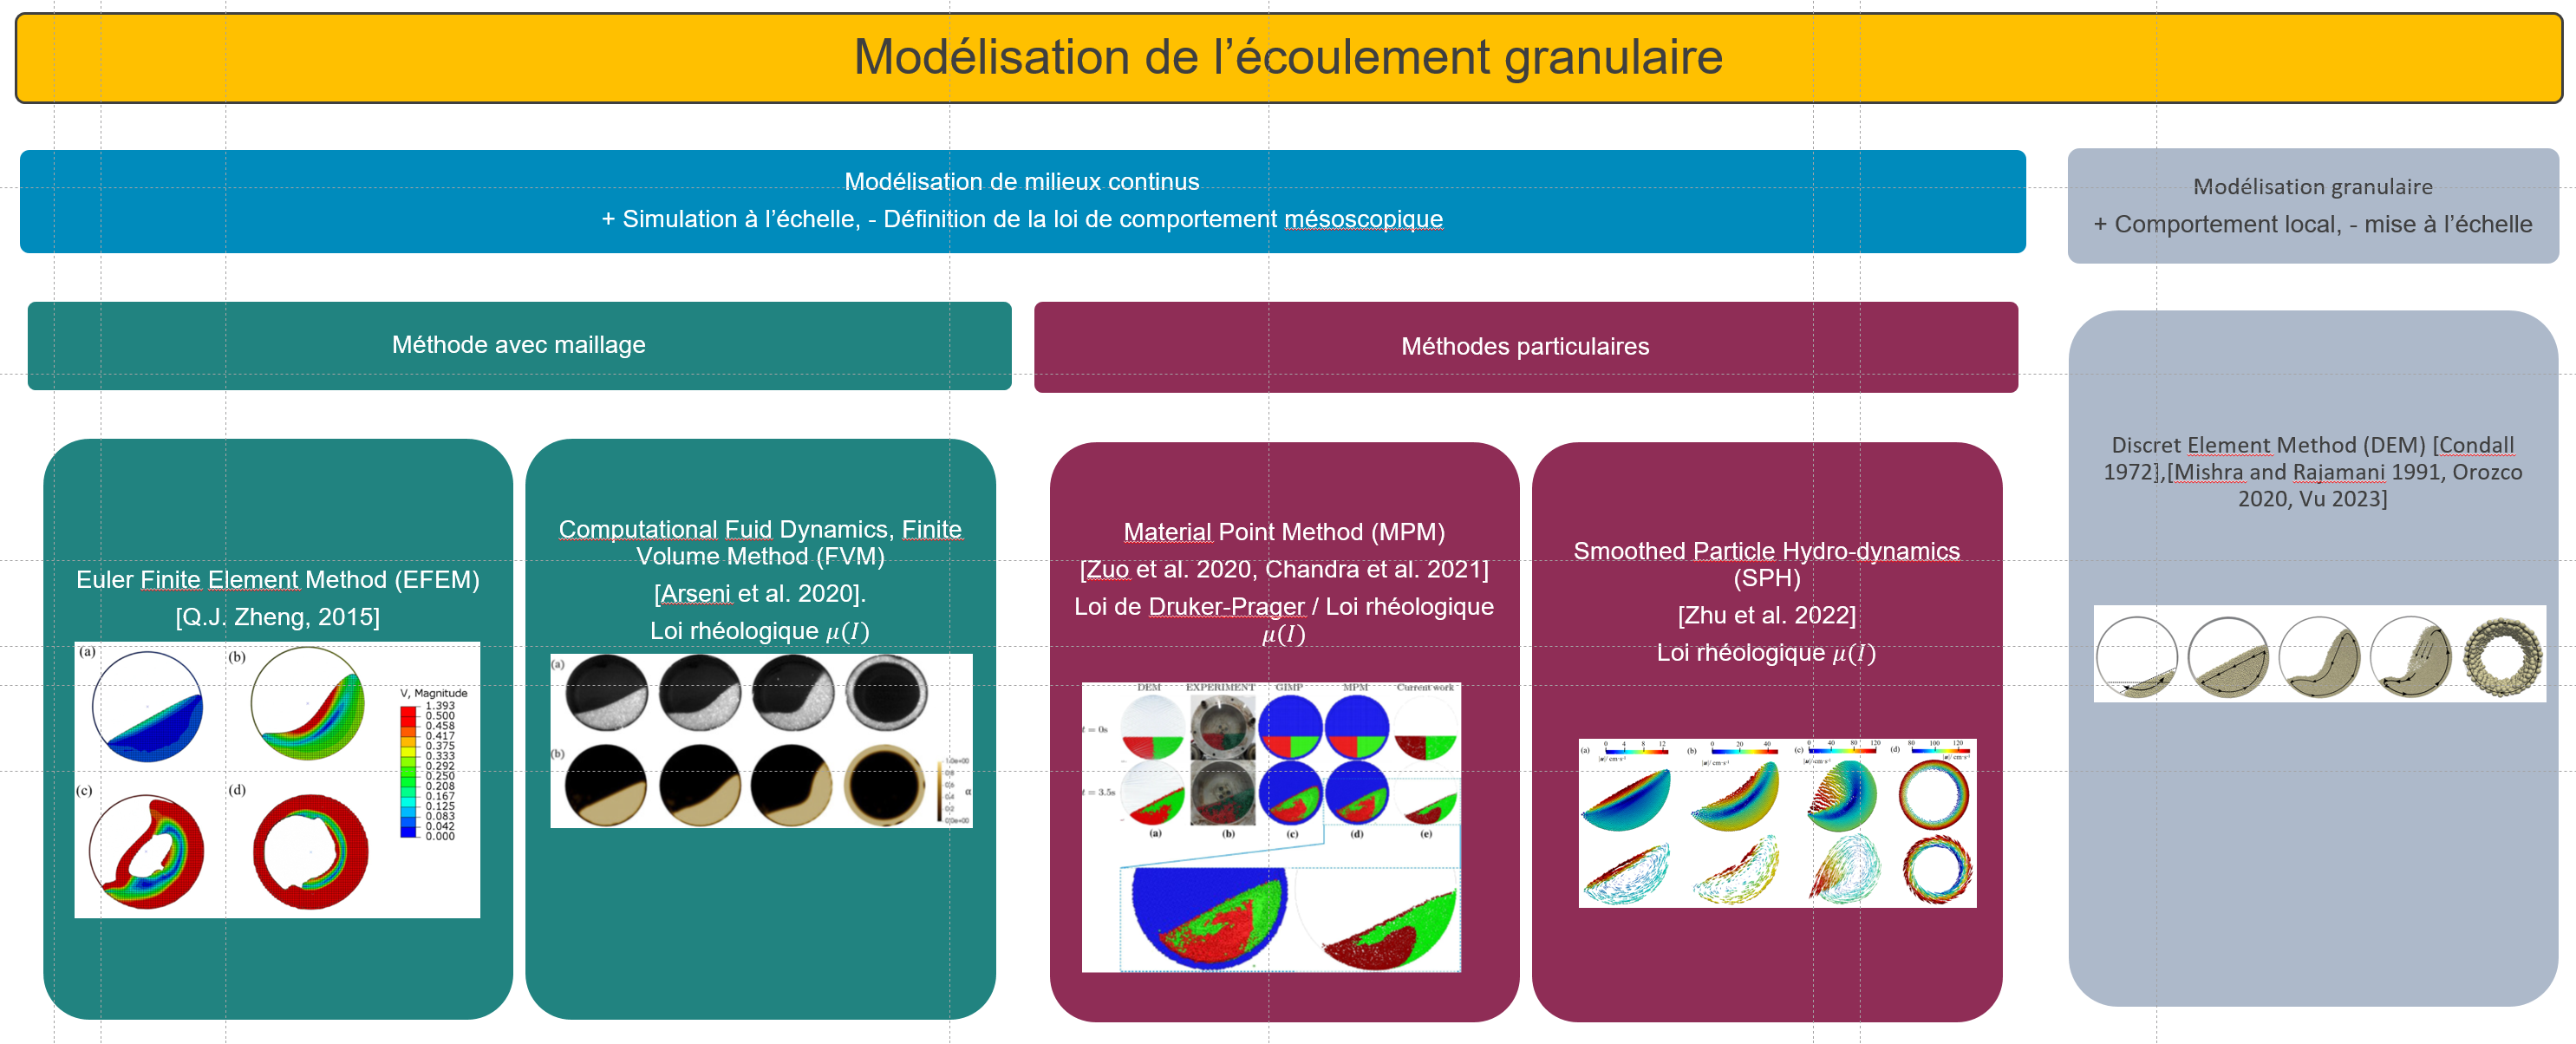
\includegraphics[width=\textwidth]{simulation_granulaire.png}
\end{figure}

\section{Mesures appliquées au tambour en rotation}~\ref{sec:mesures}

Outre l'utilisation d'outils de simulation, la validation et la compréhension du procédé se voient renforcés par l'utilisation acru de méthodes de mesure durant la phase de fonctionnement.

Ces données sont de différents types. D'une part, des données issues de l'imagerie~\cite{jarray_wet_2019,Adepu}. Celles-ci nous permetten demesurer des mesures de champ de vitesse capturées à travers la face avant d'un hublot transparent grâce à la méthode \textit{Particle Image Velocimetry} (PIV), de mesurer le ou bien de post traiter des grandeurs caractéristiques comme l'angle de repos dynamique ou de mesurer des indices de mélange.

D'autre part, des mesures accoustiques du broyeur peut révéler des informations sur divers aspects du processus, tels que les conditions de fonctionnement, les anomalies potentielles, ou encore l'usure des éléments du broyeur~\cite{Owusu, almond}.

On trouve également dans la littérature l'usage de mesure vibratoire ou de jauges de contraintes sur la paroi afin de déterminer la position du corps broyant~\cite{Davey, tano_2005}, des données issues du moteur~\cite{pedrayes_frequency_2017} ou bien l'instrumentation des boulets~\cite{Wang} (ce qui difficilement réalisable dans notre situation où la matière est contaminée).

Le laboratoire expérimental SA3E a instrumenté une maquette de broyeur dont des acquisitions sont représentées sur la Figure~\textcolor{red}{imageBastien}.

Une large gamme de mesures sont donc disponibles. Cependant, ces données mesurées ne permettent que d'avoir une représentation partielle et bruitée de l'état réel du broyage et du mélange. De plus, La qualité des résultats analysée reste néanmoins très variable. En effet, l'interprétabilité de bon nombre ce fait au travers de méthode de corrélation et non pas via des approches inductives.

Finalement, les données mesurées que nous possédons ne représentent qu'une vue brute et partielle de l'état réel, tandis que les données simulées de cet état sont sujettes à des erreurs de modélisation. Ainsi, nous souhaitons trouver un moyen d'améliorer notre connaissance des processus en tenant compte à la fois de la simulation et des mesures expérimentales.

\section{Jumeau numérique}

La notion de jumeau numérique trouve un essor considérable aujourd'hui à l'air où la données n'ont jamais été aussi présente. Le potentiel grandissant de la \textit{Big Data}, \textit{l'Internet Of Things}, le calcul haute performance (HPC) mais aussi de l'intelligence artificiel (IA) et en particulier l'apprentissage profond ouvre la voie à de nouveaux outils. Bien que sur toutes les lèvres, on trouve difficilement une définition univoque de ce paradigme.
En effet, le jumeau numérique peut être tour à tour vu comme un réplique haute fidélité capable d'émuler un système réel~\cite{noauthor_digital_nodate}, ou bien comme un modèle dynamique qui est capable d'être mis à jour avec les données de son pendant physique au long de son cycle de vie afin d'apporter une aide à la décision~\cite{AIAA2020}. Pour éviter toute confusion la distinction est souvent faite entre \textit{Virtual Twin}, \textit{Predictive Twin}, ou encore \textit{Twin Projection}~\cite{Kvamsdal}.

En définitif, le jumeau numérique n'est autre qu'un modèle, et répond au principe d'utilité énoncé par Box~\cite{box1979}: \textit{All models are wrong, some are useful}.

Le jumeau numérique pour l'étape de fabrication du combustible peu donc répondre à différents niveaux d'usages comme :
\begin{itemize}
    \item avoir une meilleure compréhension du procédé ;
    \item avoir une prédiction fidèle de l'état du système ;
    \item proposer une optimisation des paramètres de contrôle ;
    \item surveiller l'état du procédé dans une optique de maintenance prédictive ;
    \item contrôler la qualité du produit.
\end{itemize}

Finalement, le jumeau numérique peut être formalisé mathématiquement sous la forme d'un modèle graphique probabiliste proposée par Kapteyn et al.~\cite{kapteyn_probabilistic_2021}.
Elle permet de relier de bout en bout les flux de données entre capteur, et modèle numérique, mais aussi avec les paramètres de contrôle et de récompense. La représentation graphique du jumeau numérique du broyeur est présentée en Figure~\ref{fig:graph_dt}.

\begin{figure}~\label{fig:graph_dt}
    \centering
    \begin{subfigure}{0.49\textwidth}
        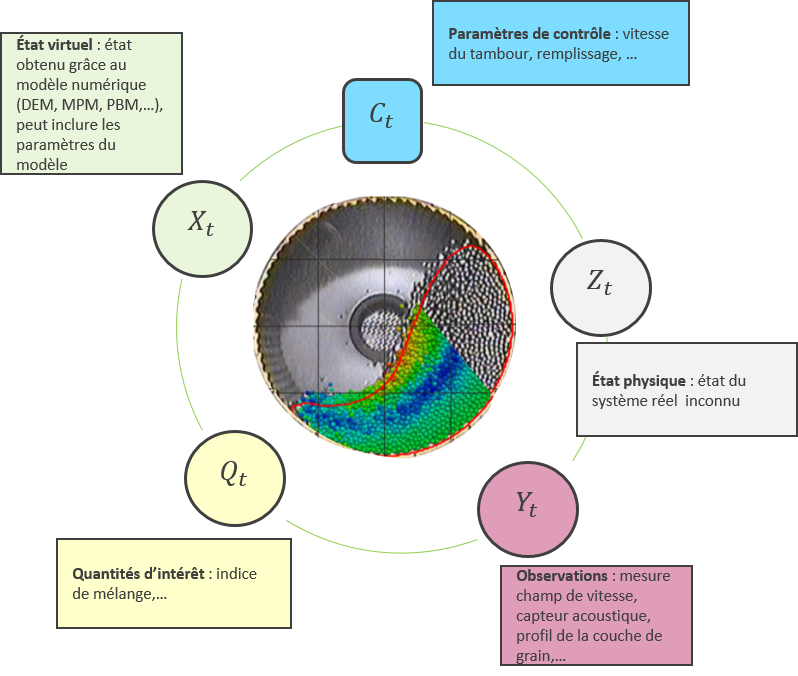
\includegraphics[width=\textwidth]{dt_broyeur.png}
    \end{subfigure}
    \begin{subfigure}{0.49\textwidth}
        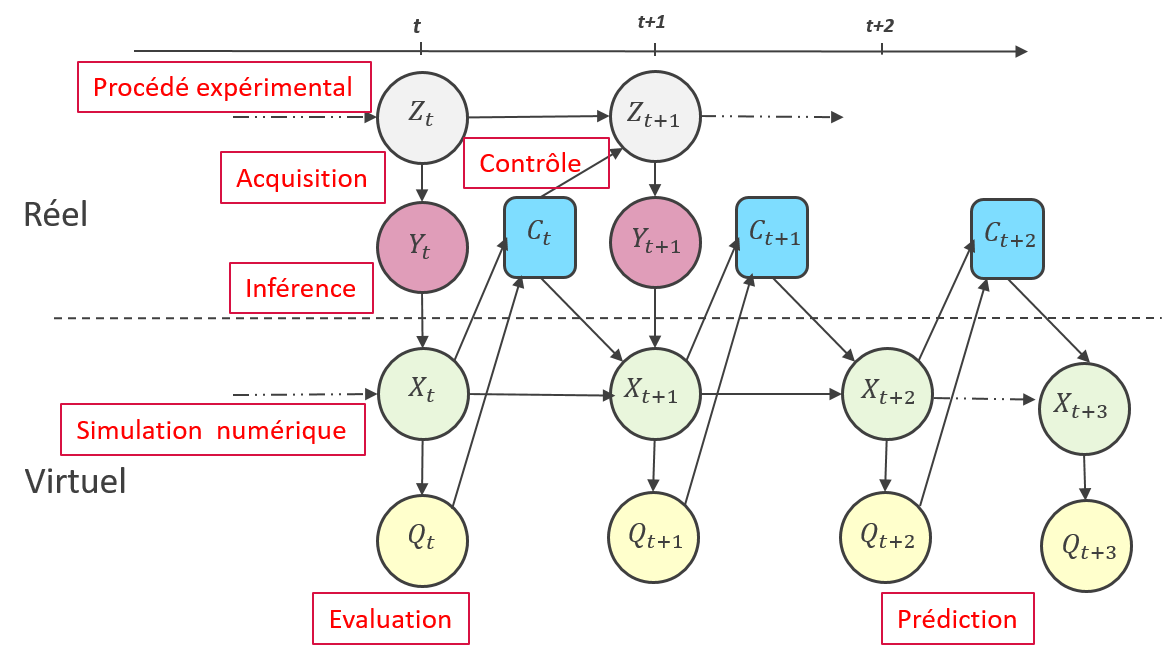
\includegraphics[width=\textwidth]{dt_seq.png}
    \end{subfigure}
\end{figure}

D'une part, on représente bien l'entité réel qui n'est connue qu'au travers des observations présentées Section~\ref{sec:mesures}. Mathématique il s'agit d'un modèle de Markov caché. D'autre part, on retrouve le modèle virtuel qui permet d'avoir accès aux variables d'intérêt et de prédire l'évolution de l'état du système à l'aide des modèles physiques comme présenté en Section~\ref{sec:simu_broyeur}
Finalement, on remarque le lien d'inférence qui permet de relier les observations et avec l'état virtuel du système. Fondamentalement, ce sont les méthode d'inférence bayésienne, et l'assimilation de données qui sont utilisés à cette étape.
Le modèle probabiliste permet ainsi d'intégrer dans la construction du jumeau numérique la notion de quantification d'incertitude.

\section{Bilan du chapitre}

Ce chapitre nous a permis de montrer la prédominance et des méthodes sans maillage pour simuler le mélange dans un tambour en rotation. Il a permis de présenter un large spectre de méthodes d'acquisition. Finalement, il a permis de présenter le jumeau numérique comme un modèle dynamique capable d'intégrer les données issues de l'observation. Ce lien est possible au travers de méthodes d'assimilation de données.





% !TEX root = ./memoire/main.tex


\section{Objectifs de la thèse}

Pour modéliser le mélange de poudre dans le broyeur à boulets intervenant dans la fabrication du combustible MOX, des simulations dites lagrangiennes ou particulaires ont été développées. D'autre part, à partir de méthodes de traitement d'images, il est également possible de mesurer des profils d'écoulement ou les champs de vitesse dans le broyeur à boulets. Pour construire un modèle de Jumeau Numérique capable d’intégrer les observations issues de l’expérience, des méthodes d'assimilation de données doivent être utilisées pour mettre à jour l'état de la simulation à partir d'observations en tenant compte à la fois des incertitudes sur l’état et les observations. Toutefois, les méthodes d'assimilation sont définies sont pour des discrétisations (maillage, grille) qui ne varient pas au cours du temps. Or les méthodes particulaires/lagrangiennes sont définies à l’aide particules qui se déplacent en suivant l’écoulement du milieu.
C'est ce qui justifie cette thèse, elle consiste à développer des méthodes d'assimilation de données adaptées à des simulations lagrangiennes.

Tout d'abord, un état de l'art respectif sur les méthodes d'assimilation de données et les simulations lagrangiennes est tout d'abord réalisé. Le chapitre~\ref{sec:prob_contribution}, offre en particulier une analyse critique sur l'adaptabilité des méthodes d'assimilation aux différents types de méthodes lagrangiennes.
%Il montrera en particulier un certain nombre de limitations, motivant le développement des contributions de thèse.
Conscient des spécificités de ce type de simulation, le chapitre suivant présentera le développement d'adaptation du filtre de Kalman d'ensemble à des simulations particulaires. Pour cela, l'idée a été de définir une correction des intensités de la discrétisation. Cette correction a été évalué sur plusieurs applications.
Dans un deuxième temps, l'objectif du chapitre qui suit a été de développer des méthode d'assimilation de donnée par correction de position pour des simulations lagrangienne. En effet, Pour cela nous formulons le problème d'assimilation de données tenant compte d'une erreur d'alignement afin d'être capable de corriger la position des particules. L'idée a été d'introduire une transformation pour aligner les particules dans un cadre variationnel.


\chapter{Outils et méthodes}
% !TEX root = memoire/main.tex

\chapter{Assimilation de données pour la construction d'un jumeau numérique}~\label{sec:da}

\section{Introduction}~\label{sec:intro_da}

La construction d'un système expert ou jumeau numérique a besoin de méthode qui puissent faire le lien entre observations et l'état de notre simulation.

En effet, les solutions calculées par les modèles numériques comportent des erreurs qu'il est crucial de comprendre, de quantifier et de réduire.

Cette incertitude peut se manifester sous diverses formes, telles que l'ambiguïté des valeurs des paramètres du modèle, l'imprécision des conditions initiales, ou l'incertitude dans la définition des conditions aux limites ou des forces extérieures. De plus, bien que les modèles numériques intègrent généralement des principes physiques essentiels, ils impliquent certaines simplifications. L'erreur numérique apparaît en raison de l'algorithme et de la discrétisation. Elle s'étend également à l'incertitude associée aux futures mesures expérimentales calibrant les modèles numériques.

En revanche, les approches stochastiques vont au-delà de la simple estimation de l'état ; elles quantifient l'incertitude associée aux états estimés. Cela est crucial, en particulier dans les systèmes dynamiques et incertains, où la reconnaissance et la caractérisation de l'incertitude deviennent primordiales pour une prise de décision fiable et l'amélioration des modèles. Dans cette approche, l'estimation est mise à jour séquentiellement en fonction des observations précédentes et actuelles. Le processus d'assimilation est réalisé dans un cadre bayésien avec une étape de prévision et une étape d'analyse. Le filtre de Kalman est un exemple de formulation séquentielle qui considère un modèle linéaire et des hypothèses de distribution gaussienne. Cependant, des filtres plus avancés ont été introduits pour s'adapter aux distributions non linéaires et arbitraires. L'un des filtres bayésiens les plus populaires est sans doute l'Ensemble Kalman Filter, introduit par Evensen, principalement en raison de son adaptabilité aux problèmes de haute dimension avec tout modèle d'évolution. Il consiste à approximer la distribution de probabilité d'un état grâce à un ensemble de simulations appelées particules ou membres.

\section{Formalisme du problème d'assimilation}

Nous décrirons le problème d'assimilation sous sa forme d'inférence bayésienne. Suivant différentes hypothèses, nous montrerons qu'elle s'exprime alors sous des formes variées.

\subsection{Définition de l'état}

Nous définissons un état $\bm z_k$ comme la variable d'\textit{état} qui représente complètement la connaissance du système à l'instant $t_k \in \mathbb R^+$. La dynamique de l'état du système au cours du temps est obtenu grâce un modèle $\mathcal{M}$ qui décrit l'évolution du système.
Nous noterons $\mathcal Z_k = \{\bz_0, \dots, \bz_k\}$ la trajectoire du modèle jusqu'au pas de temps $t_k$.
Nous supposerons que le modèle admet des incertitudes. Celle-ci sont issues de

\begin{itemize}
    \item \textbf{L'erreur de discrétisation} dans l'espace et le temps. Soit $\bz^c$ l'état réel continu. Le modèle numérique ne traite que des représentations discrètes du champ physique. Ainsi, c'est non pas l'état $\bm x^c$ qui est estimé mais une projection dans l'espace de discrétisation. On estimera $\bz^t = \Pi(\bz^c)$, où $\Pi$ est un projecteur sur l'espace de discrétisation. On parle ici d'erreur de \textit{représentativité}.
    \item \textbf{L'erreur de modèle}. C'est un modèle numérique qui calcule l'évolution de l'état simulé. Tout modèle étant imparfait, toutes les physiques ne peuvent êter prises en compte. C'est une erreur qui tient compte de la mauvaise représentation de l'évolution du système mais également de sa discrétisation.
    \item \textbf{L'erreur de données} Le modèle mathématique doit être complété par des données et des paramètres spécifiant les caractéristiques physiques du système simulé parmi la classe des systèmes représentés par le modèle. Ces données peuvent concerner la géométrie du système, les conditions aux limites et initiales, ainsi que les forçages externes. Les paramètres peuvent être des constantes physiques ou des constantes du modèle prescrivant les lois constitutives du système. L'utilisation de données qui ne reflètent que partiellement la nature du système exact induit des erreurs supplémentaires, appelées erreurs de données, sur la prédiction.
\end{itemize}

Ainsi, nous traiterons l'état comme une variable aléatoire tel que à laquelle nous lui associerons une incertitude à la prédiction $\bm \eta_k$

\begin{equation*}
    \bm z_k \mathcal{M}(\bz_0, t_k ; \bm \theta) + \eta_k.
\end{equation*}
où $\bm \theta$ sont l'ensemble des paramètres du modèle et $\bm z_0$ l'état initial.

\subsection{Définition des obervations}
A l'équation d'évolution, nous supposons également connue une équation d'émission ou équation d'observation. Celle-ci relie l'état à l'espace de mesures. On définie $\mathcal{D}_k$ les mesures prédites par la fenêtre d'état $\mathcal{Z}_k$. Tout comme l'état, les mesures sont sujettent à des incertitudes issues de plusieurs sources

\begin{itemize}
    \item \textbf{L'erreur de mesure}. L'observable $\bm y^c$ est issue d'un signal réel fonction de l'état continu $\bm x^c$. Or ce signal est mesuré par une capteur sujet à des erreurs instrumentales $\bm \varepsilon^{\mu}$. C'est une erreur intrinsèque à la méthode d'acquisition et tient compte par exemple d'interférences environnementales, du bruit électronique, ou des biais systématiques des capteurs.
    \item \textbf{L'erreur de représentativité}. L'observation est prédite par un opérateur d'observation numérique $\mathcal H$ via $\bm x_k$. Ainsi une erreur supplémentaire est induite par la représentation de l'opérateur $\mathcal H$ et celle de la projection de l'état continu avec $\Pi$. Par exemple, la discrétisation du modèle numérique ne peut pas représenter fidèlement les plus petites échelles spatiales ou temporelles présentes dans le système réel. Cette limitation entraîne une perte d'information et une simplification excessive des dynamiques fines, ce qui peut impacter directement les résultats de prédiction d'observation.
\end{itemize}

En supposant que ces erreurs sont additives, on défini la formule suivante
\begin{equation*}
    \mathcal D_k = \mathcal H (\mathcal{Z}_k) + \bm{\varepsilon}_k
\end{equation*} où $\bm{\varepsilon}_k = \bm{\varepsilon}^\mu  + \bm{\varepsilon}^r$ défini l'incertitude sur l'observation $\mathcal D_k$ relatif à la prédiction $\mathcal{Z}_k$.

\subsection{Inférence bayésienne récursive}

Le problème d'assimilation de données peut être formulé sous une approche d'inférence bayésienne. Celle-ci est une méthode statistique pour estimer l'état $\mathcal Z_k$ en utilisant à la fois une information \textit{a priori}, obtenue à partir d'un modèles et des connaissances initiales, et les données observées. Cette méthode repose sur le théorème de Bayes qui décrit la relation entre la distribution \textit{a posteriori} de l'état étant donné les données observées avec $p(\mathcal Z_k \mid \mathcal D_k)$ la distribution \textit{a priori} de l'état $p(\mathcal Z_k)$ et la \textit{vraissemblance} des données $p(\mathcal D_k \mid \mathcal Z_k)$ conditionnellement à l'état.

Cette formule est la suivante
\begin{equation*}
    p(\mathcal Z_k \mid \mathcal D_k) = \frac{(\mathcal D_k \mid \mathcal Z_k)~p(\mathcal Z_k)}{p(\mathcal D_k)}
\end{equation*}où $p(\mathcal D_k)$  est la distribution marginale des observations. Elle agit comme constante de normalization afin d'assurer que l'intégrale de la distribution a posteriori soit égale à 1.

\begin{equation*}
    p(\mathcal D_k) = \mathbb E_{\mathcal Z_k}[\mathcal D_k \mid \mathcal Z_k]
\end{equation*}

Nous souhaitons résoudre le problème d'assimilation de manière séquentielle. C'est à dire, mettre à jour l'état à chaque nouvelle observation à l'instant $t_k$. Pour ce faire, nous utilisons deux approximations

\begin{itemize}
    \item Le modèle dynamique est une \textbf{chaîne de Markov d'odre 1}. Cette hypothèse suppose que l'état futur $\bm z_{k+1}$ est indépendant des états passé $\mathcal Z_{k-1}$ conditionnellement à l'état présent $\bm z_{k}$. Le modèle dynamique s'écrit alors

          \begin{equation*}
              \bm z_k = \mathcal{M}(\bz_k ; \bm \theta) + \bm \eta_k.
          \end{equation*}

          ce qui implique mathématiquement que
          \begin{equation*}
              p(\bz_{k+1} \mid \bz_{k},\bz_{k-1}\dots \bz_{0}) = p(\bz_{k+1} \mid \bz_{k}).
          \end{equation*}

          Ainsi, la probabilité de l'état $p(\mathcal{Z}_k)=p(\bx_0, \dots, \bx_k)$ devient

          \begin{eqnarray*}
              p(\mathcal{Z}_k) &=& p(\bz_0) p(\bz_1 \mid \bz_0) p(\bz_2 \mid \bz_1) \dots p(\bz_k \mid \bz_{k-1}) \\
              &=& p(\bz_0) p(\bz_1 \mid \bz_0) \prod_{l = 1}^{k} p(\bz_l \mid \bz_{l-1}).
          \end{eqnarray*}

    \item Les observations sont indépendantes entre chaque assimilation. Cette hypothèse suppose que les observations présentes $\by_k$ soit indépendante des états et observations passé conditionnellement à $\bz_k$. Ceci correspond à définir une loi d'émission local
          \begin{equation*}
              \by_k = \mathcal H (\bz_k) + \bm{\varepsilon}_k
          \end{equation*}
          ainsi qu'une vraissemblance comme le produit de vraissemblance locale
          \begin{equation*}
              p(\mathcal{D}_k \mid \mathcal Z_k) = \prod_{l=1}^{k} p(\by_l \mid \bx_l)
          \end{equation*}
\end{itemize}

Ainsi la trajectoire de l'état et des observation suis les hypothèses d'un modèle de Markov cachés, ici à temps discret, et qui peut être schématisé par le schéma Figure~\ref{fig:hidden_markov}.

\begin{figure}[h]
    \centering
    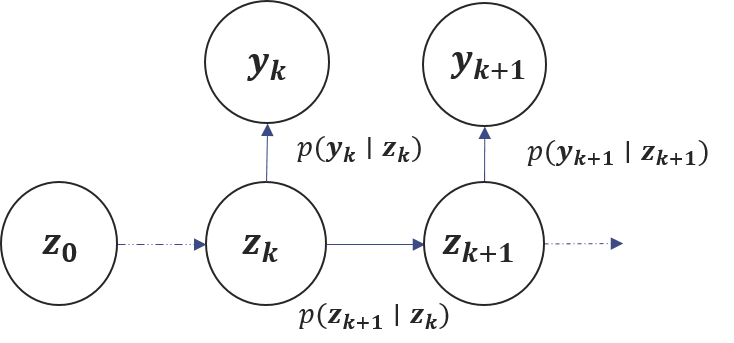
\includegraphics[width=0.5\textwidth]{hmc.png}
    \caption{Chaîne de Markov cachée}
    \label{fig:hidden_markov}
\end{figure}

On reconnait la partie inférieure du graphique présenté Figure~\ref{fig:graph_dt}.

\subsection{Estimation des paramètres du modèle par augmentation de l'état}
Nous avons supposé que le système était complètement décrit par la variable d'état $\bz$ que nous souhaitons estimé. Cependant, nous avons aussi supposé que le modèle était imparfait à cause d'erreur sur les données des paramètres de modèle. Ansi, les paramètres $\bm \theta$ ne sont pas connu avec certitude. L'estimation ou calibration de ces paramètres est possible en définissant un état augmenté $(\bz, \bm \theta)$.

Le modèle d'évolution est toutefois différent car les paramètres du modèle sont supposés constant dans le temps tel que

\begin{gather*}
    \left\{\begin{aligned}
         & \bm{z}_{k+1}      & = & \mathcal{M}(\hat{\bm{z}}_{k}) + \bm{\eta}_{k+1}    & , \\
         & \bm{y}_{k+1}      & = & \mathcal{H}(\bm{z}_{k+1}) + \bm{\varepsilon}_{k+1} & , \\
         & \bm{\theta}_{k+1} & = & \bm{\theta}_{k+1} + \bm{\xi}_{k+1}                 & .
    \end{aligned} \right.
\end{gather*}

L'ajout des paramètres dans la variable d'état a pu être utilisé pour résoudre des problème inverse sans calcul de gradient~\cite{iglesias_ensemble_2013}.

\section{Filtrage bayésien}~\label{filtrage_bayesien}

Le filtrage bayésien consiste à écrire la récurrence sur les lois de probabilité, pour estimer, en fonction des observations passées et courante $\mathcal D_k$ l'état courant $\bm z_k$ et de prédire l'état future $\bm z_{k+1}$.

Pour simplifier les notations, l'exposant $^{\mid k}$ qui conditionne la densité par les observations $\bm y_{1:N}$. La densité de l'état est initialisée par la densité a priori de l'état initial $p_{X_0}$.

Puis pour tout $k \geq 0$ les lois de probabilité sont tout d'abord propagées.

L'étape de propagation ou \textit{forecast} est obtenue grace à la loi des probabilité totales

\begin{equation*}
    p(\bm z_{k+1} \mid \mathcal D_k) = \mathbb{E}_{\bm z_k}\left[p(\bm z_{k+1} \mid  \bm z_k,\mathcal{D}_k) \mid \mathcal D_k \right] = \mathbb{E}_{\bm z_k}\left[p(\bm z_{k+1} \mid \bm z_k) \mid \mathcal D_k \right].
\end{equation*}

La loi \textit{a priori} de la $k+1$ observations peut être otenue de nouveau grace à la loi de probabilité totale

\begin{equation*}
    p(\bm y_{k+1} \mid \mathcal D_k) = \mathbb{E}_{\bm{x}_{k+1}}\left[p(\bm y_{k+1}\mid \bm x_{k+1}) \mid \mathcal D_k\right].
\end{equation*}

Après la $k+1$ observation $\bm y_{k+1}$, l'étape d'\textit{analyse}, permet grâce à la loi de Bayes de déterminer la loi \textit{a posteriori} de l'état

\begin{equation*}
    p(\bm z_{k+1} \mid \mathcal D_{k+1}) = p(\bm z_{k+1} \mid \bm y_{k+1}, \mathcal D_{k})  = \frac{p(\bm y_{k+1} \mid \bm z_{k+1} ,\mathcal D_k)  p(\bm z_{k+1}\mid \mathcal D_k)}{p(\bm y_{k+1}\mid \mathcal D_k)}.
\end{equation*}

Ainsi, les méthodes de filtrage présentent sous diverse forment ces deux étapes de propagation et de d'analyse pour mettre à jour la distribution de l'état au cours du temps et après mesure des observations.

\subsection{Propagation}
En pratique, il est difficile de réaliser la propagation de la distribution de l'état.
En effet, l'évolution du prior nécessite de propager entièrement la distribution à l'aide de l'équation de Fokker-Planck, celle-ci ne pouvant être résolue qu'en dimension faible~\cite{jazwinski_4_1970}.

Une première alternative consiste à uniquement considérer l'évolution pour les deux premiers moments. Dans ce cas, il s'agit de considérer que l'erreur de l'état $\bz_k$ suit une distribution Gaussienne $\mathcal{N} (0, \bm P_k)$. Si le modèle d'évolution $\mathcal{M} = \bM$ est linéaire, alors la matrice de covariance de l'état $\bz_{k+1}$ devient

\begin{equation*}
    \bP_{k+1} = \bM \bP_{k} \bM^T + \bm{Q_k}
\end{equation*}où $\bm Q_k$ est la matrice de covariance de l'erreur de modèle.

Cette proposition est un des éléments utilisés dans le filter de Kalman~\ref{kalman_filter}. Dans le cas où le modèle n'est pas linéaire, alors une approximation peut être obtenue par linéarisation du modèle.

Une autre possibilité consiste à utiliser un ensemble pour représenter la distribution de l'état. L'état est représenté par un ensemble d'échantillons ou particules tel que $p(\bz)  = \sum_{i=1}^{N} \omega^i \delta(\bz - \bz^i)$ est une distribution empirique de la distribution. C'est l'hypothèse qui est utilisé dans le filtre particulaire~\ref{sec:filtre_particulaire} mais également dans le filtre de Kalman d'Ensemble~\ref{sec:enkf}. Dans ce dernier cas, les membres $\bx^i$ sont supposées indépendant et identiquement distribué, ainsi les poids égaux à $1/N$.

% \subsection{Filtre particulaire}~\label{sec:filtre_particulaire}

% Le filtre particulaire est une implémentation du filtre bayésien qui approxime la PDF à l'aide d'une distribution empirique. Les transformations du filtre, \textit{forecast} et \textit{analysis} sont appliquées sur les membres de cet échantillon.
% Cette méthode converge vers la distribution exacte lorsque le nombre de particule $N \to \infty$.

% Le prior de l'état $p(\bm z)$ à l'instant $k$ est représenté par un ensemble de $N$ réalisations $\{\bm z_k^1, \bm z_k^2, \dots \bm z_k^N\}$ de tel sorte que

% \begin{equation*}
%     p_{\bm z_k}(\bm z) \simeq \sum_{i=1}^N \omega^i_k \delta(\bm x - \bm x_k^i) \quad \text{with} \sum_{i=1}^N \omega^i_k = 1, \quad \omega^i_k > 0.
% \end{equation*}

% où $\delta$ est la masse de Dirac et $\omega^i_k$ les poids associés à chaque membre. Initialement, les échantillons sont supposés tirés de manière uniforme de tel sorte que $\omega^i_k = 1/N$.

% Lors de l'étape de \textit{propagation}, les particules sont propagés par le modèle de manière déterministe.

% % Pour s'en convaincre, le loi de probabilité totale \ref{tot_rule} peut être réécrite

% % \begin{eqnarray*}
% %     p_{\bm X_{k+1}}^{\mid k}(\bm x) &=& \int p_{\bm X_{k+1}\mid \bm X_{k} = \bm x'}(\bm x) p_{\bm X_{k}}^{\mid k}(\bm x')dx' \\
% %     &\simeq& \int p_{\bm X_{k+1}\mid \bm X_{k} = \bm x'}(\bm x) \sum_{i=1}^N \omega^i_k \delta(\bm x' - \bm x_k^i) dx' \\
% %     &\simeq& \sum_{i=1}^N \omega^i_k  \int p_{\bm X_{k+1}\mid \bm X_{k} = \bm x'}(\bm x) \delta(\bm x' - \bm x_k^i) dx' \\
% %     &\simeq& \sum_{i=1}^N \omega^i_k \delta(\bm x - \mathcal M_{k,k+1}(\bm x_k^i) - \bm \eta_{k,k+1}) = \sum_{i=1}^N \omega^i_k \delta(\bm x - \bm x_{k+1}^i).
% % \end{eqnarray*}

% Quant à l'étape d'analyse, elle correspond à une mise à jour du poids de chaque membre, qui correspond à sa vraissemblance conditionnée aux données

% \begin{eqnarray*}
%     p_{\bm X_{k+1}}^{\mid k+1}(\bm x) &\propto& p_{\bm Y_{k+1} \mid \bm X_{k+1} = \bm x}^{\mid k}(\bm y)  \sum_{i=1}^N \omega^i_k \delta(\bm x - \bm x_{k+1}^i) \\
%     &\propto& \sum_{i=1}^N  \omega^i_k~p_{\bm Y_{k+1} \mid \bm X_{k+1} = \bm x_{k+1}^i}^{\mid k}(\bm y)\delta(\bm x - \bm x_{k+1}^i)
% \end{eqnarray*}

% ce qui donne

% \begin{equation*}
%     \omega^i_{k+1}  = \frac{\omega^i_k~p_{\bm Y_{k+1} \mid \bm X_{k+1} = \bm x_{k+1}^i}^{\mid k}(\bm y_{k+1}) }{\omega^j_k~\sum_j^N p_{\bm Y_{k+1} \mid \bm X_{k+1} = \bm x_{k+1}^j}^{\mid k}(\bm y_{k+1}) }
% \end{equation*}

% Où le dénominateur est simplement un terme de normalisation.

% Cependant, lorsque la dimension est grande, le nombre de poids non nulle à tendance à tendre vers 0. Pour éviter cela, des méthodes de rééchantillonnage du \textit{posterior} ont été développé. Le filtre bootstrap \cite{gordon_1993} consiste à selectionner les membres de poids les plus élevé, de les cloner de manière proportionnelle à leurs poids. Après échantillonnage, $N$ particules sont rassemblées, dont certaines sont identitiques avec des approximativement égaux.
% Un exemple d'algorithme suivant

% \begin{algorithm}
%     \caption{Implémentation du rééchantillonnage par \textit{bootstrap}.}
%     \For{membre $n$ do}{
%     Tirer $u$ dans $\mathcal{U}[0,1[$\;
%     Initialiser $j=1$\;
%     Affecter $S_w = w^1$\;
%     \While{$S_w < u$}{
%         $j = j+1$\;
%         $S_w = S_w + w(j)\;$
%     }
%     Le membre $j$  est conservé et remplace le membre $n$.
%     }
% \end{algorithm}

\subsection{Filtre de Kalman}~\label{kalman_filter}

Le filtre de Kalman introduit en 1960~\cite{kalman_new_1960} est une version du filtre Bayésien appliqué à un modèle linéaire Gaussien. Dans ces conditions, la distribution de l'état a priori de l'état et des observations sont défini par leur deux premiers moment tel que la propagation devient

\begin{eqnarray*}
    \hat{\bm{m}}_{z} &=& \bE [\bm z_{k+1} \mid \mathcal D_k] = \bm M \bm m_z,\\
    \hat{\bm  P}_{z} &=& \bV [\bm z_{k+1} \mid \mathcal D_k] = \bm M \bm m_z \bm M^T + \bm Q,
\end{eqnarray*}

et le modèle d'observation donne

\begin{eqnarray*}
    \hat{\bm{m}}_y &=& \bE [\bm y_{k+1} \mid \mathcal D_k] = \bm H \hat{\bm{m}}_{z},\\
    \bm C_{y,y}&=&\bV [\bm y_{k+1} \mid \mathcal D_k] = \bm H \hat{\bm  P}_{z} \bm H^T + \bm R, \\
    \bm C_{z,y} &=& \text{Cov}[\bm z_{k+1}, \bm y_{k+1}\mid \mathcal D_k] = \hat{\bm  P}_{z} \bm H^T,
\end{eqnarray*}

De telle sorte que la distribution \textit{a posteriori}, si cette dernière est non-dégénérée (ce qui est le cas si $\bm R$ n'est pas singulière), est défini par ses deux premiers moments qui sont

\begin{eqnarray*}
    \bm m_z &=& \bE[\bm X^{\mid k}_{k+1} \mid \bm Y_{k+1}^{\mid k}] = \hat m_X + \bm C_{X,Y} \bm C_{Y,Y}^{-1} (\bm y_{k+1} - m_Y), \\
    \bm P_{k+1} &=& \bV[\bm X^{\mid k}_{k+1} \mid \bm Y_{k+1}^{\mid k}] = \hat{\bm  P}_{k+1} - \bm C_{X,Y} \bm C_{Y,Y}^{-1} \bm C_{X,Y}^T.
\end{eqnarray*}

Ainsi la distribution a posteriori est définie comme un produit matriciel où l'estimateur a priori $\hat m_X$ et sa variance $\hat{\bm  P}_{k+1}$ sont mis à jour à partir du \textbf{gain de Kalman} $\bm K = \bm C_{X,Y} \bm C_{Y,Y}^{-1} $ et du \textbf{terme d'innovation} $(\bm y_{k+1} - m_Y)$ de telle sorte que les précédentes équations s'écrivent

\begin{eqnarray*}
    m_X &=& \hat m_X + \bm K (\bm y_{k+1} - m_Y), \\
    \bm P_{k+1} &=& (\bm I - \bm K\bm H)\hat{\bm  P}_{k+1} \\.
\end{eqnarray*}

Finalement, on peut réécrire
\begin{algorithm}
    \caption{Filtre de Kalman}
    \KwData{Initialisation de l'état $m x$ et de sa covariance $\bm P$;}
    \For{$k \geq 1$}{
        Prédiction\;
        $\hat m_x = \bm M m x $\;
        $\hat{\bm  P} = \bm M \bE [\bm X_{k+1}^{\mid k}] \bm M^T + \bm Q$\;
        Observation de $\bm Y \to \bm y$
        Analyse\;
        Calcul du gain de Kalman: $\bm K = \hat{\bm{P}}\bm H^T (\bm H \hat{\bm  P}\bm H^T + \bm R)^{-1}$ \;
        Calcul de l'analyse\;
        $m_x = \hat m_x + \bm K (\bm y - \bm H \hat m_x)$\;
        Calcul de la matrice de covariance de l'état\;
    }
\end{algorithm}

\subsection{Filtre de Kalman d'Ensemble (EnKF)}~\label{sec:enkf}

Pour surmonter les limitations du filtre de Kalman classique et du filtre particulaire, le filtre de Kalman d'ensemble (EnKF) a été développé par Evensen~\cite{evensen_sequential_1994}. L'EnKF est une méthode d'assimilation de données qui utilise un ensemble de prévisions pour estimer l'état et les incertitudes d'un système. Contrairement au filtre de Kalman classique, qui est optimal pour des systèmes linéaires et des erreurs gaussiennes, l'EnKF est plus robuste quant aux non-linéarités et aux distributions non gaussiennes.

L'EnKF fonctionne en générant un ensemble de prévisions  (ou états) $(\bx_i^f)_{i=1}^N$ à partir du modèle. Chaque membre de l'ensemble est ensuite mis à jour indépendamment en utilisant les observations disponibles. A parti de cet ensemble de représentant, supposé identiquement distribué, la matrice de covariance et la moyenne vont pouvoir être estimée.

Pour cela, nous définission la matrice d'état $\mstate_f = [\state^1, \dots, \state^N]$ et d'annomalies $\annomX_f$ dont les colonnes sont les états de chaque membre normalisé et centré ce que l'on peut écrire de la manière suivante

\begin{equation*}
    \annomX_f = \frac{1}{\sqrt{N - 1}}(\bm X_f - \overline{\state}_f \bm{1}^T),
\end{equation*}où $\bm{1} \in \mathbb{R}^N$ est un vecteur de 1.

Respectivement, la matrice d'observation et les anomalies d'observation sont $\mathcal Y_f = [\mathcal{H}(\state^1_f), \dots, \mathcal{H}(\state^N_f)]$ et $\annomY_f$, où les colonnes sont données par

\begin{equation*}
    \annomY_f = \frac{1}{\sqrt{N - 1}} \left(\mathcal Y_f - \overline{\obs}_f \bm{1}^T \right) \quad \text{avec} \quad \overline{\obs}f = \frac{1}{N} \sum{j=1}^{N} \mathcal{H}(\state^j_f).
\end{equation*}

L'ensemble définit la covariance entre les états et les observations $\Cov \bm H^T$, la covariance entre les observations $\Cov \bm H^T$, et $\tilde{\bm{K}}$

\begin{eqnarray*}
    \Cov \bm H^T &=& \frac{1}{N - 1} \sum_{i = 1}^{N} {(\state^i_f - \overline{\state}_f)}^T {\left[ \mathcal{H}_k(\state^i_f) - \overline{\bm{y}}f\right]}^T = \annomX_f \annomY_f^T, \\
    \bm H \Cov \bm H^T &=& \frac{1}{N -1} \sum{i = 1}^{N}\left[ \mathcal{H}_k(\state^i_f) - \overline{\bm{y}}_f\right] {\left[ \mathcal{H}_k(\state^i_f) - \overline{\bm{y}}_f\right]}^T = \annomY_f \annomY_f^T,\\
    \tilde{\bm{K}} &=& \Cov \bm H^T{(\bm H \Cov \bm H^T + \bm R)}^{-1} = \annomX_f \annomY_f^T {(\annomY_f \annomY_f^T + \bm R)}^{-1}.
\end{eqnarray*}

Cette implémentation sans matrice d'observation repose sur l'approximation par la méthode des sécantes $\mathcal{H}(\state^i_f - \overline{\state}_f) \approx \predi - \overline{\obs}f$.
Ensuite, la prévision est mise à jour vers un ensemble a posteriori ${[\state^i_a]}{i=1}^{N}$ tel que

\begin{equation} \label{eq:enkf_formula}
    \mstate_a = \mstate_f + \tilde{\bm{K}} ( \mdata - \mpred),
\end{equation}
où ${[\mdata]}^i = \obs + \bm{\varepsilon}^i$ est l'observation perturbée avec $\bm{\varepsilon}^i \sim \mathcal{N}(\bm{0}, \bm R) $, $\tilde{\bm{K}}$ est la matrice de gain de Kalman ensembliste et $( \mdata - \mpred)$ est le terme d'innovation.
L'étape de prévision est ensuite appliquée à l'ensemble analysé jusqu'à l'observation suivante.
Sur la base de cette formulation, nous pouvons déduire une formule de correction basée uniquement sur les prédictions des membres et les observations.

Nous pouvons réécrire la formule de mise à jour du filtre en utilisant les matrices d'anomalies précédentes.

\begin{equation*}
    \mstate_a = \mstate_f + \annomX_f \annomY_f^T {({\annomY_f \annomY_f^T + \bm R})}^{-1}(\mdata - \mpred)
\end{equation*}

Nous reformulons le terme de correction en remarquant que $ \bm{1}^T \annomY_f^T = \bm{0}$. Nous définissons $\Fcorr$, la matrice de correction qui donne la mise à jour en termes de combinaisons linéaires des états prévisionnels

\begin{equation}
    \mstate_a = \mstate_f + \mstate_f \Fcorr, \quad \Fcorr = \annomY_f^T {(\annomY_f \annomY_f^T + \bm R)}^{-1}(\mdata - \mpred).
\end{equation}

% Les équations de l'EnKF peuvent être présentées comme suit

% - **Étape de Prédiction** :
% $$x_i^f = F(x_i^a),$$
% où $x_{i}^{f}$ est la prévision du i-ème membre de l'ensemble, et $M$ est le modèle du système.

% - **Étape de Mise à Jour** :
% $$x_{i}^{a} = x_{i}^{f} + K(y_{i} - h_i^f),$$
% avec $K$ le gain de Kalman, calculé comme :
% $$K = \text{cov}(x^f, h^f)(\text{cov}(h^f, h^f) + R)^{-1}$$
% où $\text{cov}$ est l'opérateur de covariance, $(h_i^f)_{i=1}^N$ est l'ensemble d'observations prédites, et $R$ est la covariance du bruit de mesure.

Dans l'EnKF, $x_{i}^{a}$ est l'état analysé (ou mis à jour) pour le i-ème membre de l'ensemble, et $y_i$ représente les observations. Cette méthode permet de capturer la distribution de probabilité de l'état du système de manière plus efficace et avec moins de charge de calcul que le filtre particulaire, surtout dans les systèmes de grande dimension.

Cette version de l'EnKF est parfois appelé EnKF stochastique car les observations $y_i$ correspondent aux données mesurées bruitées, i.e. $y_i = y + \varepsilon_i$ où $\varepsilon_i$ correspond au bruit de mesure. Ce bruit numérique permet de supprimer un biais statistique sur l'estimation de l'état~\cite{van_leeuwen_consistent_2020}. On trouve également d'autre implémentation du filtre de Kalman d'ensemble comme le filtre EnKF déterministe comme le filtre ETKF, qui cherche une mise à jour qui permet d'obtenir une approximation de la matrice de covariance analysée du filtre de Kalman en en cherchant une racine carrée~\cite{bishop_adaptive_2001}.

\section{Méthodes variationnelles}~\label{sec:variation}
\subsection{Estimation du maximum a posteriori}

La distribution a posteriori précédemment définie permet dans un premier temps de pouvoir définir l'estimateur MAP (\textit{Maximum A Posteriori}). Il est la meilleure estimation de l'état connaissant les données mesurées. Il est défini comme

\begin{equation*}
    \bm x_{\text{MAP}} = \argmax_{\bm x} p(\bm x \mid \bm y).
\end{equation*}

Cette estimateur peut directement être déterminé directement à partir de la distribution comme avec le filtre particulaire~\ref{filtre_particulaire}.

Néanmoins, Le logarithme étant une fonction strictement croissante, la maximisation de la posterior est équivalente à minimiser $\mathcal L$. D'où la nouvelle expression de $\bm x_{\text{MAP}}$

\begin{equation*}
    \bm x_{\text{MAP}} = - \argmin_{\bm x} p(\bm x \mid \bm y).
\end{equation*}

Le MAP peut être obtenu par des méthodes d'optimisaiton numérique en fonciton de la complexité de la distribution.

Une manière de déterminer cet estimateur est d'introduire que la distribution a priori de l'état et des observations sont Gaussiennes.

Nous supposerons donc ici que les variables aléatoire introduites dans la section précédentes sont définies comme

\begin{eqnarray*}
    \bm \eta &\sim& \mathcal{N}(\bm 0, P_{k+1}), \quad p(\bm x_{k+1}) = \mathcal{N}(\bm x_{k+1}^f, P_{k+1})\\
    \bm \varepsilon & \sim & \mathcal N(\bm 0, R), \quad \quad p(\bm y_{k+1}) = \mathcal{N}(\bm g(\bm x_{k+1}^f) , R_{k+1})\\.
\end{eqnarray*}~où $\bm x_{k+1}^f = \mathcal{M}(\bx_{k})$ l'état prédit par le modèle. Nous nous interessons maintenant à l'étape de mise à jour à l'instant $k+1$, l'indice temporel sera implicite pour le reste de la section.

La distribution a posteriori peut être réécrite comme

\begin{equation*}
    p(\bm x \mid \bm y) \propto \exp\left(- \mathcal{\L}(\bm x)\right),
\end{equation*}

avec $\mathcal L(\bm x)$

\begin{equation*}
    \mathcal L(\bm x) = \frac12 \norm(\bm x - \bm x^f)_{ \bP^{-1}} + \frac12 \norm{\bm h(\bm x) - \bm d}_{\bR^{-1}}.
\end{equation*}

Le problème à minimiser devient alors

\begin{equation*}
    \bm x_{\text{MAP}} = \argmin_{\bm x} \mathcal L(\bm x).
\end{equation*}

Cette définition est à l'origine d'un ensemble de méthodes variationnelles pour l'assimilation de données dont la méthode 3DVar ou 4DVar courament utilisé en météorologie~\cite{talagrand1997assimilation}.
Le minimum de cette fonction est obtenue en annulant son gradient qui se trouve être

\begin{equation*}
    \nabla_{\bx} \mathcal L(\bx^a) = \bP^{-1} (\bx^a - \bx^f) + \nabla_{\bx^a} \bm h (\bx^a) \bR^{-1}(\bh(\bx^a) - \bm d) = \bm 0.
\end{equation*}


On peut aussi faire plusieurs remarques :

\begin{itemize}
    \item L'inverse de la dérivée seconde de la fonction coût $\mathcal L$, Hessienne, est une approximation à l'ordre 1 de la matrice de covariance a posteriori,
    \item Si l'opérateur d'observation $h$ est non linéaire alors, le problème n'est pas convexe et une méthode itérative de minimisation est souvent mis en place. Même dans le cas où $h$ est linéaire, le stockage de matrice de grande dimension peut encourager à utiliser ces méthodes itérative.
\end{itemize}

\subsection{Méthode 3DVar}~\label{subsec:3dvar}

La méthode 3DVar est un cas particulier de l'équation précédente qui permet de résoudre le problème de minimisation de la solution itérative à faible coût. Elle consiste à supposer fixe et connu les matrices de covariance $\bP$ et $\bR$. Ainsi, la matrice Hessienne $\bm B$ est donnée par $\bP$

\subsection{Equivalence avec la mise à jour de Kalman}

Elle se place dans le cas où la fonction d'observation est linéaire $\bm h(\bx) = \bH \bx$.
$$\mathcal L_{3D}(\bx) = \frac{1}{2}\norm{\bx-\bx_b}_{\bP^{-1}}^2+ \frac{1}{2}\norm{y-H(x)}^2_{R^{-1}}$$

Dans ce cas, l'annulation du gradient de la fonction coût se réduit à l'expression suivante

\begin{equation*}
    \bP^{-1} (\bx^a - \bx^f) + \bH^T \bR^{-1}(\bH \bx^a - \bm d) = \bm 0,
\end{equation*}

Ce qui nous permet d'obtenir une expression à l'estimateur MAP

\begin{equation*}
    \bx^a = \bx^f + (\bP^{-1} + \bH^T \bR^{-1} \bH)^{-1} \bH^T \bR^{-1} (\bd - \bH \bx^f),
\end{equation*}~qui est l'expression de la mise à jour dans l'espace d'état.Il peut être coûteux d'inverser la matrice $(\bP^{-1} + \bH^T \bR^{-1} \bH)^{-1}$ si l'espace d'état est de grande dimension. En appliquant deux fois la formule de Sherman-Morisson-Woodbury, si $\bP^{-1}$ et $\bR^{-1}$ sont inversibles, la mise à jour peut être réécrite dans l'espace de mesure

\begin{equation*}
    (\bP^{-1} + \bH^T \bR^{-1} \bH)^{-1} = \bP \bH^T (\bH \bP \bH^T + \bR)^{-1}
\end{equation*}

Ainsi la matrice de covariance d'état $\bP$ ne necessite pas d'être inversé. De plus on retrouve le gain de Kalman $\bK = \bP \bH^T (\bH \bP \bH^T + \bR)^{-1}$ précédemmment défini. Cette estimateur ainsi obtenu est également le BLUE (\textit{Best Linear Unbiased Estimator}). C'est en effet, l'expression est la combinaison linéaire de $\bx^f$ et $\bd$ dont l'erreur $\varepsilon^a$ est non biaisée ($\mathbb{E}[\varepsilon^a] = 0$), et dont la variance est minimale ($\Tr(\bP^a)$).

Finalement, sachant que la posterior est Gausienne, en prenant l'inverse de dérivée seconde de la fonction coût, la matrice de covariance peut être obtenue

\begin{equation*}
    (\bP^a)^{-1} = \bP^{-1} + \bH \bR^{-1} \bH^T
\end{equation*}

De nouveau avec l'identité de SMW

\begin{equation*}
    (\bm{I} - \bK \bH) \bP
\end{equation*}~qui n'est autre que la mise à jour de la covariance avec le filtre de Kalman.

\section{Méthode variationnelle d'ensemble}

\subsection{Maximum de vraissemblance échantillonné}
Les méthodes variationnelles précédemment décrite offre la possibilité de trouver le maximum d'un distribution a posteriori. Cependant, à l'aide de méthode d'ensemble, il est également possible d'estimer complètement cette distribution.

Pour cela, nous nous plaçons dans le cas d'un prior d'état Gaussien $\bm x^f$ de matrice de covariance $P^f$. On suppose $N$ échantillon i.i.d.de cette distribution $\bm x^f_i$. Après introduction de la mesure perturbée $\bm d_i = \bm d + \bm \varepsilon_i$ avec $\varepsilon_i \sim \mathcal{N}(\bm 0, \bm R)$. Alors, la distribution à posteriori peut-être échantillonnée en minimisant un ensemble de fonction coût défini pour chaque membres $i = 1, \dots, N$

\begin{equation*}
    \mathcal L_i(\bm x) = \frac12 \norm{\bm x -\bm x^f_i}^2_{\bm P^f} + \frac12 \norm{\bm h(\bm x^f_i) - \bm d_i}_{\bm R}^2,
\end{equation*}Celles-ci sont indépendantes entre chaque membre et offrent une forme similaire au MAP cette fois autour de la valeur des membres et de la mesure perturbée. Ainsi, les mêmes algorithmes de minimisation peuvent être appliqué pour résoudre ces fonctions coût.

Dans le cas linéaire et Gaussien, nous avons précedemment vu dans la Section~\ref{sec:variation} que le MAP pouvait être obtenu grâce au gain de Kalman. De même, connaissant la matrice de covariance d'état $\bm P$ et l'opérateur tangent $\bm G_i = \nabla^T_{\bx} \bm h(\bx_i)$, on obtient un ensemble de mise à jour du filtre de Kalman autour de chaque membre

\begin{equation}~\label{eq:rml-kalman}
    \bm x ^a_i = \bm x^f_i + \bm P \bm G_i^T (\bm G_i \bP \bm G_i^T + \bR)^{-1} (\bd_i - \bm h(\bx_i^f))
\end{equation}

Dans un cas non linéaire, nous pourrons traiter des cas non-linéaire pour être approchée dans un cas non Gaussien. Dans ce cas, on nous prendrons un linéarisation de la distribution a priori en estimant et ne conservant que les deux premiers moments de la distribution. C'est l'hypothèse qui est appliqué pour le filtre de Kalman d'Ensemble~\ref{sec:enkf}. De fait, cette résolution est obtenue dans un espace de représentant, offrant une optimisation dans un espace généralement de plus faible dimension.

\subsection{Méthode de rang faible}~\label{sec:faible_rang}

Nous utilisons dans cette section la même hypothèse que précédemment évoquée dans la partie sur le filtre EnKF~\ref{sec:enkf}. Il s'agit de considérer que la matrice de covariance peut etre représenté par un ensemble d'état. En fait, tout comme le filtre de Kalman et l'image du filtre 3DVar le filtre EnKF trouve une équivalence avec une approche variationnelle d'ensemble.

En utilisant les membres pour échantillonner la matrice de covariance, cela revient à chercher la solution dans l'espace vectoriel engendré par les membres.

En reprenant la formule~\ref{eq:rml-kalman}, et en remplaçant $\bm P \approx \annomX_f \annomX_f^T$, on obtient d'une part la mise à jour du filtre EnKF~\ref{enkf_formula}, d'autre part que l'on puis reformuler le terme de correction the correction term en définissant $\Fcorr$,

\begin{equation}
    \mstate_a = \mstate_f + \mstate_f \Fcorr, \quad \Fcorr = \frac{1}{\sqrt{N-1}} \annomY_f^T {(\annomY_f \annomY_f^T + \bm R)}^{-1}(\mdata - \mpred).
\end{equation}.

Ceci nous renseigne sur plusieurs choses:
\begin{itemize}
    \item La mise à jour du filtre EnKF est une combinaison linéaire des membres ;
    \item Il suffit de déterminer $N \times N$ pour résoudre le problème de mise à jour ;
    \item La mise à jour est indépendante pour les $N$ fonctions à minimiser ce qui permet de grandement paralléliser les problèmes d'optimisation.
\end{itemize}

Les $N$ problème de minimisation peuvent être reformulés à l'aide des termes de cette matrice $F$

\begin{equation*}
    \bm f_i = \argmin_{f \in } \frac12 \norm{\bm d - \bm h(\mstate_f + \mstate_f \Fcorr)}^2_{\bm R^{-1}} + \frac12 \norm{\bm f}_2^2
\end{equation*}

En effet \mycolor{mettre la formule ici}.

\section{Bilan du chapitre}
%classification des filtres

Celles-ci diffèrent par un certains nombres d'hypothèses que nous avons regroupé dans la Table et représenté sur la Figure
\mycolor{Faire un schéma des différentes méthodes de filtrage avec les hypothèses associées.}

Nous avons proposer différentes formulation du problème de filtrage. Après un rappel de la formulation bayésienne du problème, nous avons montrer que des formulations séquentielles

Dans les parties suivantes, nous présenterons quatres familles de méthode de filtrage.

\mycolor{présenter les différentes méthodes}
\begin{itemize}
    \item le filtre particulaire - filtre bayésien non linéaire sur distributions empirique
    \item filtre de Kalman - filtre bayésien modèle linéaire, distributions gaussienne
    \item Méthode Variationnelle d'ensemble - filtre non linéaire, distribution gaussienne
    \item filtre de Kaman d'Ensemble - filtre non linéaire, distribution gaussienne

\end{itemize}


% !TEX root = main.tex

\chapter{Simulation du tambour et Assimilation de données}

Nous avons vu dans le chapitre précédent que l'assimilation dépendait de la définition d'un modèle et de son état pour définir le prior et la vraissemblance. Les simulations de l'écoulement dans le broyeur à boulets qui reposent sur des discrétisations sans maillage dites particulaires, définissent ainsi notre état et son modèle d'évolution. Cependant, le caractère Lagrangien de la définition de l'état implique d'évaluer jusqu'à quel point les méthodes classiques d'assimilation peuvent être adaptée. En effet celles-ci se base sur des états dont la discrétisation restent identique. De plus, le fait que l'espace soit continu ou discret va également modifier la signification de l'état et sa capacité à être mis à jour.
Dans cette partie, nous reprendrons les principales familles de formulation particulaire en développant les formulations des méthodes DEM, SPH et MPM.  Pour chacune d'entre elles, nous évoquerons les sigularités et limites à l'adaptation des méthodes d'assimilation de données. De plus, nous présenterons la Méthode Vortex comme une méthode particulaire modèle pour la suite manuscrit.


\section{Méthode des éléments discrets (DEM)}

La méthode consiste à considérer le mouvement d'un ensemble de $N$ grains composant le milieu. Celui-ci est décrit par l'équation de la dynamique qui peut s'écrire sous la forme

\begin{equation*}
    \left\{
    \begin{aligned}
         & m_{i} \frac{ d^{2}\vec{r}_i }{dt^2}=\vec{f}_{i},\; i=1\ldots N      \\
         & I_{i} \frac{d \vec{\omega}_{i}}{dt}=\vec{\Gamma}_{i},\; i=1\ldots N
    \end{aligned}
    \right.
\end{equation*}où $`N`$ est le nombre de grains, $`m_{i}`$ est la masse, $`I_i`$ est le moment d'inertie, $`\vec{r}_{i}`$ est la position, $`\vec{\omega_{i}}`$ est la rotation, $`\vec{f}_{i}`$ est la force exercée sur le grain considéré et $`\vec{\Gamma_{i}}`$ le moment associé à la force $`\vec{f}_{i}`$.

La force $`\vec{f}_{i}`$ peut être décomposée de la manière suivante

\begin{equation*}
    \vec{f}_{i}=\underset{{\scriptstyle j\neq i}}{\sum}\vec{f}^{c}_{ij}+\vec{f}_{ext}
\end{equation*}

où $`\underset{{\scriptstyle j\neq i}}{\sum}\vec{f}^{c}_{ij}`$ représente les forces de contact qui s'exercent à la surface de la particule $i$ et les forces externes $`\vec{f}_{ext}`$ sont celles appliquées au centre de la particule $`i`$ (par exemple la force de gravité).

Les forces de contact sont décrite par des loi de contact entre les grains ainsi qu'entre les grains et la paroi. Dans le cas élastique, la modèle de Hertz est adapté pour décrire l'intéraction normale. Le modèle Hertz-Mindlin permet de déterminer les interactions tangentielles élastiques. Ces loi sont fonctions de l'interpénétration inter-particule et de la vitesse relative interpaticules. Par exemple, dans le cas de particules sphérique l'interpénétration est défini comme $\delta_{ij} = \norm{\bm x_i - \bm x_j} - (R_i - R_j)$ où $x$  est la position et $R$ le rayon d'une particule.

La force de contact tend à pénaliser l'interpénétration via des coefficients de raideur $k$ et d'amortissement $\gamma$ qui dépendent des propriétés mécaniques des grains de de la paroi. Il existe plusieurs algorithme pour résoudre numériquement les équations de la dynamique. Le plus utilisé est l'algorithme de Verlet en vitesse.


La méthode des éléments discrets (DEM, pour Discrete Element Method) est une technique de simulation numérique utilisée pour étudier le comportement des systèmes de particules, tels que lors du mélange broyage à l'intérieur du broyeur à boulets. Cette approche est particulièrement pertinente pour modéliser les interactions complexes entre les particules dans ces systèmes, où la dynamique individuelle de chaque particule peut avoir un impact significatif sur le processus global.

Dans un mélangeur-broyeur, les particules interagissent entre elles, avec les parois du broyeur, et avec le corps broyant. La DEM modélise chaque particule individuellement, en tenant compte de ses propriétés physiques telles que la taille, la forme, la masse, la rigidité, et le modèle de fragmentation. Les interactions incluent les forces de contact, les forces de frottement, et les forces de cohésion.

Le processus de simulation DEM dans un mélangeur-broyeur commence par la définition des propriétés des particules et des conditions initiales du système. Le mouvement de chaque particule est ensuite calculé en résolvant les équations de Newton pour le mouvement et la rotation. Ces calculs tiennent compte des forces et des moments résultant des collisions et des interactions entre particules, ainsi que de l'interaction des particules avec les parois du broyeur.

L'un des principaux avantages de la DEM est sa capacité à fournir des informations détaillées sur le mélange et le broyage des particules à l'échelle microscopique. Elle permet d'analyser comment les variations dans la configuration des particules, la vitesse de rotation du broyeur, et d'autres paramètres opérationnels influencent l'efficacité du broyage et l'homogénéité du mélange.

Cependant, l'utilisation de la DEM pour la simulation de mélangeurs-broyeurs peut être exigeante en termes de ressources informatiques, en particulier pour les systèmes avec un grand nombre de particules.


\subsection{DEM et assimilation de données}

L'assimilation de données, lorsqu'appliquée à des systèmes simulés par la méthode des éléments discrets (DEM), se heurte à plusieurs limites importantes présentées ci-dessous.

\subsubsection{Limites de la DEM avec les méthodes variationnelles}

Dans le cadre des méthodes variationnelles d'assimilation de données, telles que 3D-Var, le principal défi est la grande dimensionnalité du problème d'optimisation.
En effet, La DEM simule le comportement de chaque particule individuellement. Cela signifie que l'état du système comprend les variables cinématique de chacune d'elles : position, la vitesse, accélération mais aussi la position angulaire, la vitesse angulaire et l'accélération angulaire ou la densité de chaque particule. Pour un système avec des milliers voire des millions de particules, cela conduit à un problème d'optimisation de très grande dimension.

De plus, il existe un nombre extrêmement élevé de contraintes, notamment l'interdiction de l'interpénétration des particules. Ces contraintes doivent être prises en compte pour assurer que la solution d'optimisation soit physiquement admissible.

L'application des méthodes 3D-Var et 4D-Var est donc trop exigeante d'un point de vue des temps de calcul.

De plus, les filtres variationnels corrigeant des erreurs d'intensité selon des normes euclidiennes, la variation selon les positions des observations ne sera pas linéaire.

Ainsi, la définition d'un état de particules discrètes implique de résoudre un problème d'optimisation non-linéaire de grande dimension.

\subsubsection{Limites de la DEM avec EnKF}
Pour l'EnKF, l'état estimé du système est une combinaison linéaire des états prédits par les différents membres de l'ensemble. Cependant, dans le contexte de la DEM, cette combinaison linéaire des états n'est pas nécessairement physiquement admissible. Par exemple, elle pourrait conduire à des situations où les particules s'interpénètrent ou violent d'autres lois physiques.
En d'autres terme, la mise à jour ne peut être réalisé que via le solveur lui-même capable de vérifier des contraintes de non interpénétrabilité mais ne peut être réalisé directement.

Un autre problème avec l'EnKF dans le contexte de la DEM est la difficulté de faire correspondre les particules entre les différents membres de l'ensemble. Même si initialement chaque membre possèdait la même configuration particulaire mais avec des propriétés différentes, chaque particule a sa propre trajectoire unique en cohérence avec les intéractions dans son voisinage. Aligner ces trajectoires à travers les différents membres de l'ensemble pour une assimilation de données cohérente est un défi complexe. Cette difficulté est exacerbée par le nombre élevé de particules et par la nature dynamique et chaotique de leurs interactions.

Dans le cas pus général où les membres n'aurait pas le membre de particule la correspondance des états est d'autant plus complexe.

Ainsi, le caractère discret de la méthode DEM rend l'assimilation par EnKF à la fois complexe par :

\begin{itemize}
    \item une définition de l'état et de ses statistiques non univoque ;
    \item la construction du gain de Kalman d'Ensemble ;
    \item la contrainte d'interpénétration lors de la mise à jour.
\end{itemize}

\section{Méthodes particulaires continues}
\subsection{Méthodes basées sur les particules}~\label{Background_Part}
Nous envisageons des méthodes par particules pour résoudre des problèmes continus en mécanique des fluides ou des solides. Cela inclut des méthodes telles que l'hydrodynamique par particules lissées (SPH) \cite{lucy_1977,gingold_monaghan_sph_1977} et la méthode des vortex (VM) \cite{cottet_vortex_2000}, et s'étend à d'autres méthodes comme la méthode des points de matériau (MPM) \cite{sulsky_particle_1994}. Elles partagent toutes de décomposer cette fois le domaine en un ensemble $\mathcal{P}$ de particules qui suivent la dynamique du problème. Ainsi, la discrétisation suit la transformation appliquée au milieu en transportant des quantités attachées à chaque particule. Elles sont en cela des méthodes Lagrangienne.

\subsubsection{Discrétisation par particules}

La solution représentée par le jeu de particule est obtenue grâce à deux éléments: une appproximation grâce à un noyau de lissage et l'approximation particulaire d'un opérateur intégral. Si la représentation de la solution peut évoluer suivant la méthode (en particulier avec la méthode MPM), la solution peut toujours être exprimé de cette manière suivant le choix du noyau.

Tout champ relativement régulier $\bm{u}$ sur $\Omega$ peut être écrit grâce à la propriété de filtrage de Dirac

\begin{equation*}
    \bm{u}(\bm{z}) = \int_{\Omega} \bm{u}(\bm{z'}) \delta(\bm{z'} - \bm{z})  d\bm{z'},
\end{equation*}avec $\delta$ la distribution de Dirac.

Une fonction de noyau $\phi_\varepsilon$ est introduite pour obtenir une estimation moyenne $\langle \bm{u} \rangle$ de $\bm{u}$ telle que

\begin{equation*}
    \langle \bm{u}(\bm{z}) \rangle = \int_{\Omega} \bm{u}(\bm{z'}) \phi_\varepsilon(\bm{z}-\bm{z'}) d\bm{z},
\end{equation*}où $\varepsilon$ est la longueur de lissage. Le noyau lisse doit au moins respecter les propriétés suivantes

\begin{eqnarray*}
    && \int_{\Omega} \phi_\varepsilon(\bm{z}) d\bm{z} = 1,      \\
    && \phi_\varepsilon(\bm{z}) \to \delta(z), \quad \varepsilon \to 0, \\
    && \phi_\varepsilon(\bm{z}) \in C^k,  \quad k \geq 1,
\end{eqnarray*} où les deux premières propriétés sont des propriétés résiduelles de la distribution de Dirac et la dernière est une exigence de différentiabilité nécessaire pour approcher les opérateurs différentielles.

La fonction moyenne $\langle \bm{u} \rangle$ est ensuite utilisée pour approximer la fonction d'origine.

Dans un second temps, le domaine d'origine $\Omega$ est subdivisé avec $N_p$ sous-domaines $\Omega_p$ associés à une particule Lagrangienne à l'emplacement $z_p \in \Omega_p$. Nous notons $V_p$ le volume de $\Omega_p$. Cette discrétisation est ensuite utilisée pour approximer la fonction moyenne de telle sorte que

\begin{eqnarray*}~\label{part_approx}
    \langle \bm{u}(\bm{z}) \rangle &=& \sum_p \int_{\Omega_p} \bm{u}(\bm{z'}) \phi_\varepsilon(\bm{z}-\bm{z'}) d\bm{z'} \\
    &\approx& \sum_p \bm{u}(\bm{z}_p) V_p \phi_\varepsilon (\bm{z}-\bm{z}_p) \\
    &\approx& \sum_p \bm{U}_p \phi_\varepsilon (\bm{z}-\bm{z}_p).
\end{eqnarray*}

Ainsi, toute fonction définie sur une discrétisation par particules est définie par un ensemble de positions de particules $\bm{z}_p$ associées à une valeur de particule $\bm{U}_p = \bm{u}(z_p) V_p$ et un noyau lisse $\phi_\varepsilon$.

Sur la base de cette discrétisation, l'opérateur différentiel peut être dérivé à travers cette formulation.

Tout comme le champ $\bm u$, la même interpolation peut être appliquée pour obtenir

\begin{equation*}
    \nabla \bm{u}(\bm{z}) = \sum_p \bm{U}_p \nabla \phi_\varepsilon (\bm{z}-\bm{z}_p).
\end{equation*}

Ils existent toutefois une grande variété de formule pour approximer l'opérateur gradient. Dans ces cas, ce sont les propriétés de conservation associées au champ qui sont privilégiées.
Généralement, un terme additionnel est introduit lorsque le champ est évalué à la position d'une particule $q$ tel que

\begin{equation*}
    \nabla \bm{u}(\bm{z}_p) = \sum_q (\bm{U}_q - \bm{U}_p) \nabla \phi_\varepsilon (\bm{z_q}-\bm{z}_p)
\end{equation*}, où $\sum_q \bm{U}_p \nabla \phi_\varepsilon (\bm{z_q}-\bm{z}_p)$ est nul par propriété de localisation du noyau $\phi_\varepsilon$.

\subsubsection{Exemple de fonctions de noyau}

Plusieurs noyaux ont été utilisés en fonction de la méthode. La formulation originale de la MPM n'utilisait pas de noyau de substitution et écrivait la densité comme suit

\begin{equation*}
    \bm{u}(\bm{z}) = \sum_p \bm{U}_p \phi_\varepsilon (\bm{z}-\bm{z}_p)
\end{equation*}

Et la résolution est basée sur une projection sur une grille de fond associée à certaines fonctions de forme \cite{sulsky_particle_1994}.

La méthode GIMP est une formulation différente qui utilise la fonction de Heaviside \cite{bardenhagen_generalized_2004} et associe donc un volume autour de chaque particule

\begin{equation*}
    M_1(r) = \frac{\alpha}{\varepsilon}\left\{\begin{aligned}
         & 1; & r \leq \varepsilon \\
         & 0; & \text{sinon}
    \end{aligned}
    \right.
\end{equation*}où $r = \norm{\bm{z}}_2$.

Cette méthode a été introduite pour éviter le problème de passage de cellule lorsque une particule se déplace d'une cellule à une autre à travers la grille de fond.

Dans la méthode SPH, comme son nom l'indique, un noyau lisse est associé pour approximer la solution. Théoriquement, il pourrait s'agir de la fonction de noyau gaussien

\begin{equation*}
    \phi_g(r) = \frac{1}{{(\pi \varepsilon^2)}^{d/2}} \exp(-r^2/\varepsilon^2)
\end{equation*}.

Ce noyau est infiniment différentiable mais défini sur un support non compact. En pratique, nous utilisons une coupure pour supprimer les valeurs négligeables pour une grande distance par rapport à une particule.

D'autres noyaux, basés sur des fonctions B-Spline pour travailler sur un support compact. Ces fonctions sont également positives, ce qui est une exigence pour certains champs comme la densité.

Par exemple, le B-spline quadratique, que nous appelons $M_3$, est défini avec
\begin{equation}~\label{quadratic_kernel}
    M_3(r) = \frac{\alpha}{\varepsilon^d}\left\{ \begin{aligned}
         & \frac{3}{4} - |q|^2                            & 0 \leq           & |q| < \frac{1}{2} \\
         & \frac{1}{2} {\left(\frac{3}{2} - |q|\right)}^2 & \frac{1}{2} \leq & |q| < \frac{3}{2} \\
         & 0                                              & \frac{3}{2} \leq & |q|
    \end{aligned}
    \right.
\end{equation}avec $r = \norm{z}_2 $ et $q = r / \varepsilon$ et $\alpha$ la condition de normalisation et $d$ la dimension spatiale.

Ce noyau garantit la continuité $C^1$.
Le noyau cubique est un autre noyau B-Spline qui est
\begin{eqnarray}~\label{cubic_kernel}
    M_4(r) &=&  \frac{\alpha}{\varepsilon^d} \left\{ \begin{aligned}
         & \frac{1}{6}{(-|q|+2)}^3 - \frac{4}{6}{(-|q|+1)}^3 & 0 \leq      & |q| \leq  1 & \\
         & \frac{1}{6}{(- |q|+2)}^3                          & 1      \leq & |q| \leq 2  & \\
         & 0                                                 & 2 \leq      & |q|
    \end{aligned}
    \right.
\end{eqnarray}

Dans ce dernier cas, le facteur de normalisation $\alpha$ est

\begin{equation*}
    \alpha = \left\{ \begin{aligned}
         & 1;    \quad      & 1\text{ d} \\
         & 30/14 \pi; \quad & 2\text{ d} \\
         & 3/ 2\pi; \quad   & 3\text{ d}
    \end{aligned}
    \right.
\end{equation*}

Notez que ces noyaux ont été définis avec la coordonnée radiale $r$. Une autre possibilité serait de définir le noyau multidimensionnel comme le produit tensoriel du noyau 1D

\subsection{SPH}

La méthode SPH a étét développée indépendemment par Lucy~\cite{lucy_1977}, et Gingold et Monhagan~\cite{gingold_monaghan_sph_1977}. Elle a été formulé initialement pour dess problème de formation et d'évolution des systèmes stellaires. Tout comme en mécanique quantique sont but est de réprésenter le système discret en le lissant pour obtenir un milieu continu discrétisé par un ensemble de particules. En mécanique, cette méthode est vu comme une méthode de discrétisation sans maillage d'un milieu continu.
Elle consiste à résoudre la forme forte des équations de la dynamique en approchant les champs et les opérateurs différentiels à l'aide de l'approximation particulaire et l'approximation par noyau précédemment évoqué.

Les équations résoluent sont l'équation de continuité et l'équation de conservation de la quantité de mouvement à travers l'équation d'Euler

\begin{eqnarray*}
    \frac{d\rho}{dt} + \rho \nabla \cdot \bm{v} = 0, \\
    \frac{d\bm v}{dt} = \frac1\rho \nabla \cdot \bm \sigma,
\end{eqnarray*}où $\rho$ est la densité, $\bm v$ la vitesse, $\bm \sigma$ la contraite de Cauchy.

En utilisant la règle d'approximation du gradient le terme $\rho \nabla \cdot \bm{v}$ peut être approximé pour chaque particule, ce qui donne pour l'équation de continuité

\begin{equation*}
    \frac{d\rho_p}{\sum_{q} m_j (\bm v_j - \bm v_i) \cdot \nabla \phi_\varepsilon(\bm z_p - \bm z_q)}.
\end{equation*}

De la même manière, l'équation d'équilibre des quantités de mouvement peut êter discrétisé. La forme suivante est généralement utilisée

\begin{equation*}
    m_p \frac{d \bm v}{dt} = \sum_{q} m_p m_q \left(\frac{\bm \sigma_p}{\rho_p^2} + \frac{\bm \sigma_q}{\rho_q^2} \right) \cdot \nabla \phi_\varepsilon(\bm z_p - \bm z_q).
\end{equation*}

Cette version est symétrique par rapport aux indices $p$ et $q$ ce qui favorise les propriétés de conservation.

Finalement, les équations de la dynamique sont intégrées dans le temps généralement à l'aide d'un algorithme dit \textit{leap-frog}.

\section{Méthode des points matériaux (material point method, MPM)}

La méthode des points matériaux (MPM) est une technique de simulation numérique innovante, particulièrement adaptée à la modélisation de phénomènes complexes comme ceux rencontrés dans les mélangeurs-broyeurs. Cette méthode représente un compromis entre les approches par éléments finis et par particules, offrant ainsi une modélisation efficace des interactions matérielles dans des environnements dynamiques et déformables.

Dans la MPM, l'intérieur du tambour d'un mélangeur-broyeur est conceptualisé comme un milieu continu, adoptant une perspective macroscopique. La réponse du milieu est alors représenté par une loi de comportement mécanique telle que la loi de Drucker-Prager. Cela contraste avec la méthode des éléments discrets (DEM), qui se concentrent sur les interactions particule-par-particule.

Le processus de simulation avec la MPM implique des itérations entre une grille de calculs et des particules matérielles. Chaque particule porte des informations essentielles associées au matériau, telles que la masse, le volume, et les propriétés mécaniques (variables internes, gradient de déformation...). Ces particules sont utilisées pour transférer des informations sur et hors d'une grille de calculs, où les équations de mouvement et de comportement du matériau sont résolues.

Cette approche hybride permet à la MPM de capturer efficacement les déformations importantes, les ruptures, et d'autres comportements complexes du milieu qui sont fréquents dans les opérations de mélange et de broyage. En revanche, la description fine du phénomène proposée par la DEM n'est plus disponible.

En termes de temps de calculs, la MPM est plus efficace que la DEM.

\subsection{La MPM et la DA}
La MPM offre un cadre exploitable pour mettre en place une méthode de DA.
La structure de grille sous-jacente à la MPM permet une modélisation l'utilisation des méthodes variationnelles ou des méthodes d'ensemble. La structure de particules est aussi plus flexible dans le sens où elles représentent une densité de matière : elles peuvent donc s'interpénétrer.

\subsubsection{MPM et méthodes variationnelles}
Le principal défi est de gérer la dimension du problème d'optimisation pour la 3D-Var, ainsi que construire un modèle adjoint pour la 4D-Var.
Deux pistes sont envisageables : mettre à jour les champs nodaux et les champs particulaires. Comparativement à la DEM, le nombre de variables et le nombre de contraintes sont drastiquement réduits au prix d'une représentation plus grossière.

\subsubsection{MPM et EnKF}
Pour l'EnKF, l'état estimé est une combinaison linéaire des états prédits. Dans le contexte de la MPM, cela signifie que la mise à jour de l'état peut être directement effectuée sur la grille de calcul, plutôt que sur les particules individuelles. Cette approche réduit la complexité des calculs et facilite l'assimilation de données dans des systèmes à grande échelle.

Cependant, l'intégration de la MPM avec l'EnKF soulève plusieurs questions importantes :

1. **Transfert d'Informations de Particules à la Grille** : La première question concerne le transfert efficace des informations des particules vers la grille. Cela nécessite des algorithmes précis pour garantir que les informations pertinentes sur les propriétés des matériaux, telles que la densité, la contrainte, et le gradient de déformation déformation, sont correctement représentés sur la grille de calcul.

2. **Remaillage de Particules pour Représenter l'État Mécanique** : Une autre question clé est de savoir comment effectuer un remaillage des particules pour représenter fidèlement l'état mécanique du système après assimilation. Cela est crucial pour maintenir la cohérence et l'exactitude du modèle MPM, en particulier après des mises à jour successives de l'état du système.

Au travers des précédentes méthodes particulaires, nous constatons que l'application des méthodes d'assimilation sont innégalement applicable. En particulier, les méthodes discrètes n'offre pas la possibilité de corriger directement l'état de la discrétisation, mais nécessite une correction au travers du schémas d'intégration. D'autre part, les méthodes particulaires continues (par exemple MPM, SPH), permettent de modifier et faire varier dans son intégralité la discrétisation particulaire. En effet, chaque particule est définie en un point, ce qui annule tout problème d'interpénétration. Toutefois, il reste nécessaire de définir les
Afin de facilité le développement de nouveaux filtres, une autre méthode particulaire a été utilisée la méthode Vortex. Elle a été choisie car elle offre une modélisation plus simple que les méthodes SPH et MPM. En effet, chaque particule ne transporte qu'une quantité scalaire.Toutefois, elle dispose de toutes les caractéristiques d'une méthode particulaire continue. On retrouve de plus différentes version de cette méthode. Ainsi, la formulation classique de la méthode se rapproche de la méthode SPH et la méthode Vortex-In-Cell de la méthode MPM en mécanique des solides.

\section{Méthode Vortex}

La méthode Vortex (VM) est une méthode particulaire utilisé pour résoudre  dans le cas d'écoulements incompressibles~\cite{Cottet_Koumoutsakos_2000}. Elle a été pour la première fois développé indépendemment par Prager~\cite{prager1928druckverteilung} et Rosenhead~\cite{rosenhead1931formation}. Elle se base sur la discrétisation du champ de vorticité par un ensemble de particules, et résoud la formulation vorticité-vitesse des équations de Navier-Stokes

\begin{eqnarray*}
    \frac{\partial \bm \omega}{\partial t} + (\bm{u} \cdot \nabla) \bm \omega - \nu \Delta \bm \omega & = 0, \\
    \nabla \cdot \bm u  & = 0,
\end{eqnarray*}avec $\omega$ pour la vorticité, $\bm{u}$ la vitesse et $\nu$ pour la viscosité.

Dans le cas d'un écoulement bi-dimentionnel, la vorticité définie comme $\nabla \wedge v$ peut être défini comme un scalaire selon la troisième coordonnée. En particulier dans un repère cartésien $\omega = \frac{\partial v_y}{\partial x} - \frac{\partial v_x}{\partial y}$.

Le champ de vorticité est discrétisé à l'aide d'un ensemble de particules $p$ défini à une position $\bm z_p$, une quantité de circulation locale $\Gamma_p$ qui qui est par définition la circulation autour de la particule : $\Gamma_p = \oint_{\partial \Omega_p} \bm v = \int_{\Omega_p} \omega dS$. Ainsi, pour tout point $z \in \Omega \subset \mathbb R^2$ la vorticité peut être exprimée comme

\begin{equation*}
    \omega(\bm z, t) = \sum_{i=1}^{N_p} \Gamma_p(t) \phi_\varepsilon(\bm z - \bm z_p(t)),
\end{equation*}où $\phi_\varepsilon$ est le noyau associé à la particule avec une distance de lissage $\varepsilon$.

Dans le cas non visqueux, c'est à dire $\nu = 0$, la position des particules $\bm z_p$ au temps $t$ est obtenue en résolvant l'équation

\begin{equation*}
    \frac{d\bm z_p(t)}{dt} = \bm u (\bm x_p(t), t).
\end{equation*}

D'auter part, la circulation restant constante au cours du temps sur une courbe fermée, $\Gamma_p$ satisfait en 2D

\begin{equation*}
    \frac{d\bm \Gamma_p(t)}{dt} = 0.
\end{equation*}

La vitesse $\bm u$ peut être obtenue en résolvant l'équation de Poisson suivante

\begin{equation*}~\label{eq:poisson}
    \lambda \bm u = - \nabla \wedge \omega.
\end{equation*}

Finalement, par une représentation intégrale et en choisissant $\phi= \delta$, on obtient dans le cas 2D l'équation de Biot-Savart suivante

\begin{equation*}
    \bm u(\bm z) = \sum_p \frac{\Gamma_p}{2\pi}  \bm k \wedge \frac{\bm z - \bm z'}{\|\bm z - \bm z'\|^2},
\end{equation*}où $\bm k$ est le vecteur unitaire normal au plan.

En pratique, le choix d'un noyau en Dirac rend ainsi impossible le calcul de la vitesse sur la discrétization particulaire à cause du dénominateur. En choisissant un noyau de type gaussien de taille $\varepsilon$ on obtient alors

\begin{equation*}
    \bm u(\bm z) = \sum_p \frac{\Gamma_p}{2\pi r^2} \bm k \wedge (\bm z - \bm z')(1 - \exp(-r^2 / \varepsilon^2)), \quad r = \|\bm z - \bm z'\|.
\end{equation*}

Afin de tenir compte de la diffusion, une approche par fractionnement est généralement utilisé. Introduite pour la première fois par Chorin~\cite{chorin_discretization_1973}, elle permet dans le cas de problème où le terme de transport est dominant, de traiter séparemment et successivement les termes d'advection et de diffusion.

Ainsi après avoir mis à jour la position des particules sans tenir compte de la viscosité, l'équation suivante est résolue

\begin{equation*}
    \frac{d\bm omega_p}{dt} = \nu \Lambda \omega(\bm x_p).
\end{equation*}

Pour se faire, deux méthodes sont principalement utilisées : soit la méthode par marche aléatoire introduite dans~\cite{chorin_discretization_1973} ou échange d'intensité introduite par~\cite{1989MaCom..53..485D}.
Dans le premier cas, la position de chaque particule est perturbée avec un vecteur de variables indépendantes tirées selon une distribution gaussienne de moyenne zero et d'écart-type $2\nu \Delta t$. Dans le second cas, l'opérateur différentiel est approximé à l'aide de la discrétisation comme il est fait dans la méthode SPH.

\subsection{Vortex-In-Cell, VIC}

La méthode Vortex-In-Cell~\cite{christiansen_1973} est une version Particle-In-Cell~\cite{birdsall_1969} de la méthode Vortex précédemment décrite. Elle a été développé pour tenir compte de ses faiblesses. Tout comme la méthode MPM, celle-ci tient bénéfice de la représentation particulaire des particules pour tenir compte du terme d'advection mais également d'une grille de calcul pour résoudre l'équation de Poisson ou le terme de diffusion en utilisant des méthodes eulérienne.

Le schéma de transfert est similaire d'avec celui de la méthode MPM. D'abord une projection du champ de vorticité sur la grille (p2g) pour obtenir les valeurs nodales $\omega_i$. L'équation de Poisson~\ref{eq:poisson} est résolue sur la grille, soit par différences finies, soit par une méthode FFT pour obtenir des vitesses au noeud $\bm u_i$. La vitesse est ensuite interpolée sur le particule (g2p) pour mettre à jour leur position (advection).

Avec de la diffusion, l'équation de diffusion peut être ensuite résolue sur la grille et interpolé pour mettre à jour les quantités particulaire.

\subsection{Similarité avec les méthodes SPH et MPM}
Cette approche diffère de la MPM dans le sens où les particules portent des informations complexes sur les propriétés mécaniques du matériau.

Le processus de simulation avec la VIC implique d'abord le calcul des champs de vitesse sur la grille. Ces champs sont ensuite utilisés pour déplacer les particules dans le fluide, qui à leur tour transportent la vorticité à travers le domaine de simulation. L'avantage de cette méthode est sa capacité à modéliser avec précision les phénomènes complexes d'écoulement de fluides, tels que la formation et l'évolution de tourbillons, tout en maintenant une structure de calcul relativement simple.



% !TEX root = ./memoire/main.tex
\chapter{Méthodes particulaires et assimilation de données}~\label{sec:prob_contribution}

\textcolor{red}{à compléter}
L'assimilation de données, lorsqu'elle est appliquée à des systèmes simulés par des méthodes lagrangiennes, se heurte à plusieurs limites importantes. A la fois pour les méthodes variationnelles (ex : 3DVar) ou stochastique (ex : EnKF) il faut considérer deux problématiques majeurs : la définition de l'état et la manière de le mettre à jour.
Nous évoquerons les singularités et limites à l'adaptation des méthodes d'assimilation de données. Cependant, ces problématiques trouvent un echo dans le reste de la littérature en particulier pour des problèmes à maillage adaptatif, lorsque les observations sont des données lagrangiennes ou lorsqu'une erreur de position doit être prise en compte. Finalement, nous présenterons la démarche de notre contribution.

\section{Problématique et revue bibliographique}

\subsection{Définition de l'état d'une méthode particulaire}~\label{sec:etat_meshless}

L'état est une représentation de toutes les variables pertinentes du système à un instant donné. Il est souvent représenté par un vecteur d'état $\bm z$ comme dans la Section~\ref{sec:da}. Pour les états continues, comme des champs de densité ou de vitesse dans notre cas, des méthodes de discrétisation sont utilisées. Elles sont essentielles pour la résolution numérique et permettent habituellement d'exprimer le vecteur d'état $\bm z$. Les méthodes classiques de simulation en mécanique vont utiliser un représentation fixe pour définir un espace de représentation fonctionnel.


On considère un domaine $\Omega \subset \mathbb R^d$, soit $\mathcal{T} = (\mathcal N, \mathcal E)$ un maillage, où $\mathcal N = \left\{\bm x_i \right\}^n_{i=1}$ est l'ensemble des nœuds, et $\mathcal{E} = \{ K_i \}_{i=1}^{m}$ l'ensemble des éléments.

\begin{itemize}

    \item \textbf{La méthode des éléments finis(FEM)}~\cite{fem} associe à chaque nœuds $i$ des fonctions de forme $\phi_i$.
          L'état de la solution \(u_h\) discrétisé peut alors être définie comme

          \begin{equation*}
              u_h(\bm x) = \sum_{i=1}^{N} u_i \phi_i(\bm x),
          \end{equation*}où $u_i$ les valeurs nodales à déterminer. Le vecteur d'état est défini sur les nœuds du maillage $\bz = \{ u(\mathbf{x}_1), \dots, u(\mathbf{x}_n)\}$

    \item \textbf{Méthode des volumes finis (FVM)}~\cite{fvm}, la solution est approximée par une valeur moyenne sur chaque élément $K_i$ comme

          \begin{equation*}
              u_i = \frac{1}{\lvert K_i \rvert}\sum_{i=1}^{m} \int_{K_i} u~\text{d}K
          \end{equation*}

          de telle sorte que la solution approchée est une solution constante par éléments

          \begin{equation*}
              u_h(\bm x) = \sum_i^m u_i \mathbb{1}_{K_i}(\bm x).
          \end{equation*}

          Il est alors possible de définir l'état comme une variable aléatoire  $\bz = \{ u(K_1), \dots, u(K_m)\}$.

    \item \textbf{méthode d'interpolation à fonctions de base radiale(RBF)} Tout comme les méthodes particulaire, la méthode d'interpolation RBF paramétrise les fonctions de base radiale $\phi$ par une position $\bm x_i$ et des paramètres de forme $\theta$ tel que

          \begin{equation*}
              u_h(\bm x) = \sum_{i}^n u_i \phi_i(\bm x; \bm x_i, \theta),
          \end{equation*}où $u_i = u(\bm x_i)$. Si $\phi$ est une fonction définie strictement positive, et $\bm x_i$ distinct, alors $u_h$ est bien défini de manière unique par les valeurs nodales. Ainsi l'état peut être défini comme $\bz = \{ u(\bm{x}_i) \}_{i=1}^{n}$
\end{itemize}

Les discrétisations étant fixes, il n'est pas nécessaire d'inclure la position des nœuds ou des éléments pour représenter l'état. Finalement, le modèle est résolu au cours du temps grâce à des équations différentielles tel qu'il est possible d'écrire $\frac{d \bm z}{dt}(t) = \mathcal M (\bm z(t); \mathcal D) $où $\mathcal D$ la discrétisation utilisée.

Dans le cas des méthodes lagrangiennes particulaires, la situation est différentes. En effet, Le support de discrétisation, porté par les particules, évolue également au cours du temps. L'état ne peut donc pas être défini uniquement par les valeurs d'intensité, mais doit considérer également les positions des particules.

Une première solution consiste à considérer chaque particules indépendamment dans la définition de l'état en associant position et intensité.

\begin{itemize}
    \item Pour la DEM, l'état à l’instant $t$, pourrait alors être défini comme
          \begin{equation*}
              \bz(t) = {(\bx_p(t), \bm v_p(t), \bm \theta_p(t), \bm \omega_p(t), A_p)}_{p=1}^N
          \end{equation*}où $N$ le nombre de grains, et présente à la fois les variables cinématiques ainsi que $A_i$ les propriétés intrinsèques de la particules comme sa masse ou sa géométrie.

    \item De même pour les méthodes particulaires continues, par exemple la méthode vortex, l'état peut être défini comme

          \begin{equation*}
              \bz = {(\bx_p(t),\bm \Gamma_p(t), A_p)}_{p=1}^{N_p}
          \end{equation*}où cette fois $A_i$ défini en particulier les propriétés de la fonction de lissage.
\end{itemize}

Dans ces cas, on peut en effet définir la fonction approchée $u_h$, et définir un modèle d'évolution pour l'état $\bm z$ comme décrit en Section~\ref{sec:simu_part}. Cette définition de l'état a en particulier été utilisé~\cite{chen_superfloe_2022} pour une méthode DEM appliquée au mouvement de la banquise ou bien avec la méthode vortex~\cite{darakananda_data-assimilated_2018,le_provost_ensemble_2021}. Ce sont des filtres EnKF qui ont été développés dans ces deux cas.

Toutefois, cette définition peut être assez contestable dans le cas général. Premièrement, il est alors nécessaire de faire l'hypothèse que tous les membres possèdent le même nombre de particules dans un ordre défini. Dans le cas contraire il n'est pas possible de réaliser le calcul des statistiques sur l'ensemble. Il est néanmoins possible d'ajouter des particules supplémentaires à la suite des précédentes dans le vecteur d'état en remplissant de valeurs nulles le cas échéant. Cependant, le risque est de voir le nombre de particules augmenter considérablement après mise à jour, ou de ne pas pouvoir représenter convenablement les statistiques de l'état discrétisé. Cette remarque est d'autant plus sensible en considérant le caractère chaotique d'un problème à N-corps~\cite{poincare1890}. En effet, dans ce cas, deux particules proches à une perturbation près peuvent, en un temps fini, voir leur trajectoires totalement décorrélée. Le système peut conserver une régularité dans sa globalité, mais il devient tout à fait incongru de continuer à comparer ces deux particules entre elles. Ainsi, il n'est plus possible de définir l'état comme selon une collection de particules individuelles ou bien de définir des statistiques qui est un sens pour une particule données.
%Finalement, pour les méthodes continues, on a une relation entre statistique du champ $u_h$ et état discret $\bm z$ qui est non linéaire. Par exemple, pour la moyenne
Dans les articles~\cite{chen_superfloe_2022} ou~\cite{darakananda_data-assimilated_2018} cette première limitation a été traité en regroupant les particules pour en obtenir des systèmes de plus faible dimension. Dans le premier cas, il s'agit de créer des superstructures de glace, dans le second cas, il s'agit d'utiliser des méthodes d'agglomération de vortex. L'assimilation de données est donc appliquée au détriment du niveau de détail des solutions.

En particulier, on obtient différent estimateurs Monte-Carlo avec les méthodes d'ensemble. En supposant un ensemble de champs $\{u_i\}_{i=1}^N$, de vecteur d'état associé $\left\{z_i = \left\{\bx_{ip},\bm \Gamma_{ip}\right\}_ {p \in \mathcal P}\right\}_{i=1}^N$, on obtient deux estimateurs Monte-Carlo pour la moyenne

\begin{eqnarray*}
    \mathbb{E}(u(\bm x)) \simeq e_1(\bm x) =\frac{1}{N} \sum_{i=1}^N u_i(\bm x) = \frac{1}{N} \sum_{i=1}^N \sum_{p \in \mathcal P}\bm \Gamma_{ip} \phi_\varepsilon(\bm x - \bx_{ip}), \\
    e_2(\bm x) = \sum_{p \in \mathcal P} \mathbb{E}(\bm \Gamma_{p}) \phi_\varepsilon\left(\bm x - \mathbb{E}(\bx_{p})\right) =\frac{1}{N} \sum_{i=1}^N \sum_{p \in \mathcal P} \bm \Gamma_{ip} \phi_\varepsilon(\bm x - \bar{\bx}_{p}),
\end{eqnarray*} où $ \bar{\bx}_{p} = \frac1N \sum_{i=1}^{N} \bx_{ip}$. Du fait de la non-linéarité du noyau, on obtient deux estimateurs différents.
\subsection{Mise à jour de l'état d'une simulation particulaire}

% \subsubsection{Pour les méthodes variationnelles}
Une autre problématique majeur est celle de la mise à jour de l'état lors de l'analyse. Une première limitation concerne les méthodes variationnelle comme la méthodes 3DVar présentée en~\ref{subsec:3dvar}. D'une part, l'opérateur d'observation $\mathcal H(z)$, est non-linéaire par rapport aux variables particulaires tel que la position $\bx_i$. Pour un système avec des milliers voire des millions de particules, on se retrouve à traiter un problème d'optimisation fortement non-linéaire dans un espace de très grande dimension. De nouveau, on pourrait procéder à une réduction du nombre de particules. Toutefois, dans le cas des méthodes discrètes, il est nécessaire de prendre en considération un nombre élevé de contraintes. Notamment, le déplacement des particules doit respecter l'interdiction d'interpénétration des particules. Cette conditions doit être vérifié sur l'ensemble du système pour assurer que la solution d'optimisation soit admissible. Dans le cas des méthodes continues, les particules sont des entités ponctuelles et ne représentent qu'une discrétisation d'un milieu continu. Ainsi cette dernière contrainte ne s'applique pas. Finalement, utiliser une méthode d'assimilation de données variationnelles dans le cas d'une discrétisation particulaire nécessite de traiter une problème d'optimisation non-linéaire de grande dimension avec contraintes pour la méthode DEM et sans contrainte dans le cas continu.

% \subsubsection{Pour la méthode EnKF}
Dans le cas de la méthode EnKF, la mise à jour est définie de manière statistique. De ce fait, elle ne tient pas compte de contraintes physiques. L'équation~\ref{eq:corr} montre en effet, que l'état estimé lors de l'analyse est une combinaison linéaire des états prédits par les différents membres de l'ensemble, en particulier sur les positions des particules $\bx_i$.
En DEM, bien que chaque membre vérifie les conditions de non interpénétration, ces conditions n'étant pas linéaire, il n'y a aucune garantie pour que la combinaison le soi. En d'autres terme, la mise à jour ne peut être réalisé que via le solveur lui-même capable de vérifier des contraintes de non interpénétration mais ne peut être réalisé directement. Dans le cas de l'article~\cite{chen_superfloe_2022}, si le filtre EnKF a pu être utilisé, c'est en parti car le critère non interpénétration est relaxé.

Si cette problématique ne concerne pas les méthodes particulaires continues, il reste toutefois questionnable de réaliser une combinaison linéaire des positions des particules. Cette question est en fait en lien avec la définition de l'état. En effet, chaque particule n'est que le support de la discrétisation d'un champ continu. Mesurer une erreur quadratique sur la position des particules n'aura pas de lien linéaire avec l'erreur quadratique sur le champ.

\textcolor{red}{Ceci est relativement vrai pour un champs d'un problème tournant. La rajouter une exemple, présente un cas où chaque membre discrétise un même champ de tourbillon mais où le support de discrétisation a plus ou moins de retard.}.
Encore une fois, une solution consiste à réaliser des agrégations pour regrouper les particules comme en~\cite{chen_superfloe_2022,darakananda_data-assimilated_2018} mais au détriment du détail de discrétisation.

% Finalement, la mise à jour en considérant des discrétisations particulaires est complexe. En DEM elle doit prendre en considération les positions relatives des particules entre elles. De manière générale, nous avons vu que considérer les statistiques sur les positions de particules ne permettait pas d'avoir une bonne idée de l'incertitude sur le champ discrétisé. Ainsi, il nous semble nécessaire de formuler différemment le problème d'assimilation dans le cadre d'un discrétisation particulaire pour tenir compte

Finalement, l'assimilation de données pour les méthodes particulaires souffre d'un certain nombre de limitations lié à la discrétisation lagrangienne de la solution. Pour les méthodes discrètes comme la DEM, la principale difficulté consiste à devoir prendre en compte les contraintes de distance entre particulaire, ce qui complique à la fois la mise à jour avec les méthodes stochastiques et variationnelles. De manière générale, il faut tenir compte de la variabilité dans les positions de la distribution particulaire. La non-linéarité de la solution par rapport aux positions limite l'applicabilité des méthodes classiques pour l'assimilation de données. Ainsi, il devient nécessaire de proposer des méthodes d'assimilation de données, qui soient adaptées au problème de discrétisation particulaire. D'une part, en considérant pour les méthodes ensemblistes, que chaque membre dispose d'une distribution de particule qui lui est propre. D'autre part, que le traitement de la mise à jour des positions et des intensités doit être différentiés.

\section{Revue bibliographique}

Ces limitations ne sont pas toute propre uniques à ce domaine, mais se retrouvent également dans d'autres disciplines. Le fait d'avoir un ensemble de membre ne partageant pas les mêmes discrétisations est aussi une problématique pour l'application du filtre EnKF avec des méthodes de maillages adaptatifs. De même, la même problématique de passé d'une représentation eulériennes, c'est à dire sur une grille fixe vers une représentation lagrangienne a également dû être considéré pour des observables. Finalement,

\subsubsection{Assimilation de données sur maillages adaptatifs}

Les méthodes particulaires continues peuvent être considérées comme le choix d'une discrétisation mobile d'un problème continu. Ainsi, en utilisant un ensemble de simulations basées sur ces méthodes, on se heurte aux mêmes problématiques que celles rencontrées avec des simulations utilisant des maillages adaptatifs.
Dans ce cas le principal défi réside dans le fait que les dimensions de l'espace d'état changent au cours du temps et diffèrent d'un membre de l'ensemble à l'autre. Cette variabilité complique les opérations ensemblistes habituelles, telles que les calculs matriciels, lors de la mise à jour de l'analyse.

Une solution courante consiste à adopter une discrétisation de référence commune à tous les membres. Dans les méthodologies à grille fixe avec l'analyse multi-résolution (MRA) et dans les scénarios de maillage mobile, les états définis sur des grilles variées sont harmonisés à travers des techniques de projection et d'interpolation pour établir une grille de référence destinée aux mises à jour des états \cite{siripatana_combining_2019, bonan_data_2017}. Cette démarche offre une grande flexibilité, permettant diverses combinaisons de grilles de référence et de mise à jour adaptées aux spécificités des données et des objectifs de l'étude. Par ailleurs, Siripatana et al. \cite{siripatana_combining_2019} soulignent que la correction par le Filtre de Kalman d’Ensemble (EnKF) repose uniquement sur les prédictions et les observations, indépendamment de la définition de l'état. En réalité, cela simplifie l'application de l'EnKF dans des contextes où les maillages varient entre les membres de l'ensemble en proposant une correction qui est indépendante de la discrétisation

\subsubsection{Méthodes d'assimilation pour des données lagrangiennes}
\textcolor{red}{présenter des méthodes dans des cas où les variables sont des quantités lagrangiennes}

D'autre part
- Méthodes particulaires sont des méthodes lagrangiennes
- Avoir données variable problématique déjà traité par des données océanographiques issu de flotteurs par exemple
- Pour traiter ce type de problème, une première approche initialement développé dans~\cite{ide_2002}, est d'augmenter le vecteur d'état ici noté $\bm x$ avec les données d'observation de position de traceur. Cependant, cette variable étant fortement non-linéaire, l'application d'un filtre de Kalman étendu (linéarisation du filtre de Kalman) ne converge pas si les observations ne sont pas suffisamment fréquente. Finalement, cela revient à définir l'état comme dans la Section~\ref{sec:etat_meshless} précédente, ce qui n'est pas adéquat.

L'utilisation d'une méthode de type état augmenté trouve plus de sens pour l'application de méthode variationnel.
C'est en particulier ce qui est proposé dans les travaux de Apte~\cite{apte_2008} pour le filtre 3DVar et le ceux de Nodet~\cite{nodet_2006} pour le filtre 4DVar incrémental.

Cependant, ici les quantités lagrangiennes sont des quantités passives, c'est à dire qu'elles n'interviennent pas dans la résolution du champ de vitesse à intégrer. Dans notre cas les traceurs sont des supports de discrétisation de la solution. De ce fait, le modèle adjoint du modèle n'est pas aussi simple à construire car la position des particules impactent le champ de vitesse à intégrer.


\subsubsection{Méthodes d'assimilation de données par déplacement ou alignement}~\label{sec:biblio_align}

Dans le Chapitre~\ref{sec:da}, nous avons présenté l'assimilation de données comme la combinaison les simulations issues d'un modèle avec les données bruités issues de l'observation. Cette combinaison nécessite de pouvoir mettre à jour de manière optimale l'état de la simulation en tenant compte à la fois de l'erreur \textit{a priori} du modèle ainsi que l'erreur d'observation. Plus précisément, ces méthodes cherchent à déterminer la distribution ou l'estimateur du maximum a posteriori (MAP) de l'état par correction de l'intensité.

Cependant, on trouve de nombreuses limitations à ces schémas classiques, en particulier lorsqu'il existe une erreur de position. En effet, les méthodes d'assimilation de données classiques sont construites en mesurant l'erreur à l'aide d'une norme quadratique qui tend à sur pénaliser des erreurs issues d'alignement. Pour s'en rendre compte, on peut constater en Figure~\ref{fig:double_penalization_error} qu'une erreur sur l'alignement sera sur-pénaliser en comparaison de l'erreur avec une solution nulle. On parle d'effet de \textit{double pénalisation} car cette effet intervient à la fois pour l'évaluation de l'erreur sur le modèle mais également sur les observations~\cite{amodei2009}. C'est d’ailleurs une des contribution majeur à l'erreur de représentativité~\cite{janjic2018}.

\begin{figure}[h]
    \centering
    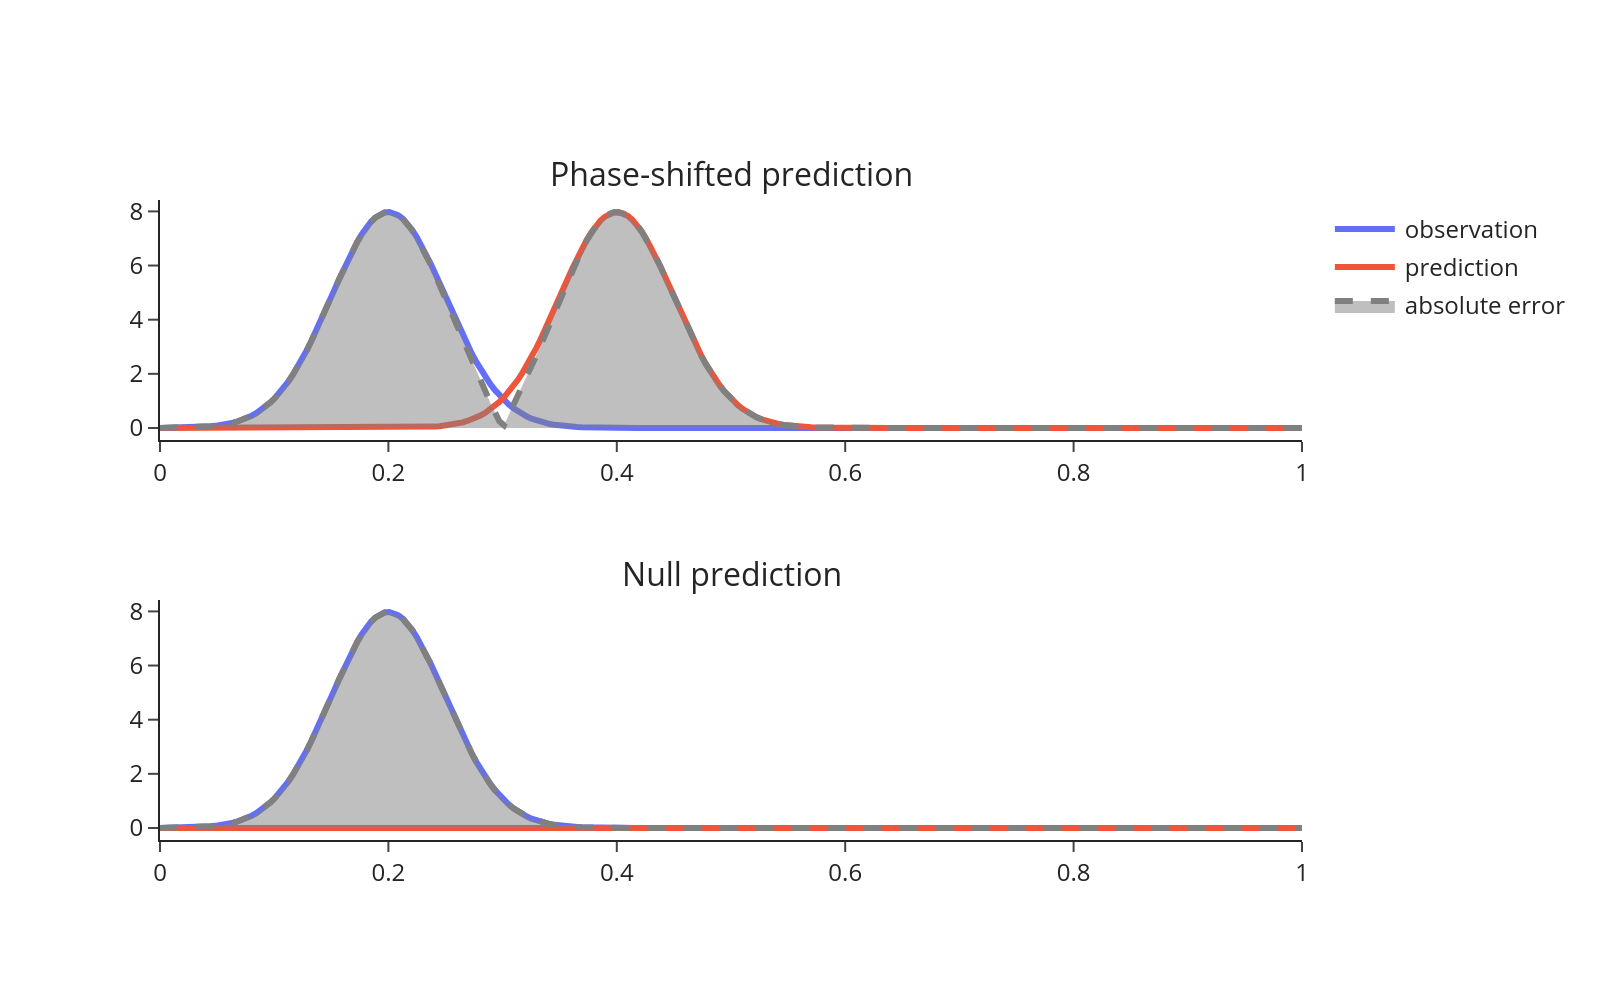
\includegraphics[width=\linewidth]{double_penalisation.png}
    \caption{Visualisation de l'effet de double pénalisation.}~\label{fig:double_penalization_error}
\end{figure}

Un seconde limitation, concerne la nécessité pour les champs d'état et d'observation \textit{a priori} de recouvrir la solution à analyser. En effet, la mise à jour des méthodes d'assimilation de données classique consiste essentiellement à un interpolation dans l'espace des valeurs des champs, produisant ainsi une analyse encore confinée dans le support de l'état de fond et celui de l'observation. Cette remarque est d'autant plus flagrante dans le cas du filtre EnKF qui se défini justement comme combinaison des membres de l'ensemble comme décrit en Section~\ref{sec:enkf}. Cette limitation est donc tout à fait en lien avec notre problème de support de discrétisation particulaire.


Pour résoudre ce problème plusieurs approches ont pu être proposées. Une première manière assez élégante est de s'inspirer de méthode de transport optimal pour définir une correction dans un espace d'interpolation plus riche et prenant en compte des déplacements~\cite{villani2009optimal,benamou_computational_2000}. Ceci passe par substitution de la norme quadratique par une norme de Wasserstein. Ainsi les travaux de thèse de Feyeux~\cite{feyeux_transport_2016} ont permis d'utiliser une distance de Wasserstein pour l'assimilation de données issues d'images. L'article de Bocquet et al. \cite{bocquet_bridging_2023} propose quand à lui une adaptation de la méthode 3D-Var au transport optimal.En particulier, son approche s'applique à des distributions d'état et d'observation de masses potentiellement différentes. Bien que les algorithmes de transport optimal ait gagnés en efficacité computationnel~\cite{cuturi_2014,peyre_cuturi_2019,Simsekli2018SlicedWassersteinFN}, ils restent encore difficilement applicable dans le contexte de l'assimilation de données.

Si le transport optimal permet en effet de réaliser simultanément des corrections en intensité et en position, on trouve un certain nombre de développement qui introduisent des transformations spatiales. En particulier Percival et al.~\cite{percival_department_2008} utilisent des idées en théorie du réarrangement afin d'appliquer une transformation de coordonnées. Ravela et al.~\cite{ravela_data_2007} introduisent de leur côté une variable de déplacement pour ainsi corriger indépendamment position et intensité. Cette méthode à aussi été adaptée dans une formulation multi-échelle~\cite{ying_multiscale_2019,ying_improving_2023}. Finalement, Rosenthal et al.~\cite{rosenthal_displacement_2017} présente une méthode séquentielle en deux étapes pour aligner et corriger les intensité successivement. L'objectif est alors de conserver des propriétés morphologiques de tourbillon. Pour cela, la correction est réalisée en appliquant une transformation cinématiquement admissible pour corriger la position, puis une correction d'intensité. L'avantage de cette méthode est qu'elle offre la possibilité de la coupler aux méthodes classiques d'assimilation.

C'est donc dans la continuité de ces travaux, et en particulier ceux de Rosenthal, que nous souhaitons proposer une méthode de correction de distribution particulaire des simulations sans maillage.

\section{Contributions}

\textcolor{red}{Présenter les méthodes que j'ai mis en place.}
\section{Bilan du chapitre}

Au travers des précédentes méthodes particulaires, nous constatons que l'application des méthodes d'assimilation sont inégalement applicable. En particulier, les méthodes discrètes offre difficilement la possibilité de corriger directement l'état de la discrétisation, et nécessite une correction au travers du schémas d'intégration pour éviter des problèmes d'interpénétration. Dans la suite, nous nous focaliserons sur les méthodes particulaires continues.

D'autre part, les méthodes particulaires continues (par exemple MPM, SPH), permettent une plus grande flexibilité des schémas d'assimilation. En effet, chaque particule est définie en un point, ce qui annule tout problème d'interpénétration.

Dans tous les cas, ce sont des méthodes qui ont la particularité d'avoir des discrétisations variables au cours du temps. Cela vient de la représentation lagrangienne sous-jacente. Cela rend difficile l'application de méthodes ensemblistes comme la méthode EnKF ou des opérations de calcul matriciel doivent être réalisé entre membres.

D'autre part, ce sont des méthodes dont les opérateurs d'observation sont hautement non-linéaire par rapport aux positions des particules. Ainsi, cela complexifie l'application de méthodes variationnelles qui doivent construire des modèles adjoints pour des méthodes particulaires de grande taille.

Ainsi il devient assez claire que positions et intensités de particule ne peuvent pas être traité de la même manière. Ainsi en s'inspirant des méthodes d'assimilation sur des maillages adaptatifs ou multi résolution, on proposera des méthodes d'assimilation ensembliste qui mettrons à jour les intensités.

Dans un second temps, on proposera plutôt des approches variationnelles pour traiter de la correction des positions de particule.

Afin de facilité le développement de nouveaux filtres, nous avons utilisé la méthode vortex. Elle a été choisie car elle offre une modélisation plus simple que les méthodes SPH et MPM. En effet, chaque particule ne transporte qu'une quantité scalaire, une quantité de tourbillon. Toutefois, elle dispose de toutes les caractéristiques d'une méthode particulaire continue avec à la fois une formulation classique de la méthode se rapproche de la méthode SPH et la méthode Vortex-In-Cell de la méthode MPM.


\chapter{Adaptations du filtre EnKF pour des simulations lagrangiennes par correction d'intensité}

% \begin{abstract}
% This study presents a novel approach for integrating data assimilation techniques into particle-based simulations using the Ensemble Kalman Filter. If data assimilation methods have been applied to Eulerian simulations for a long, they have never been properly used in the context of a Lagrangian solution discretization. Two specific methodologies are introduced to complete the analysis. The first one is based on the use of an intermediary Eulerian transformation combining a projection and a remeshing process. The second is a purely Lagrangian scheme that is applicable when remeshing is not adapted. These methods are evaluated using a one-dimensional advection-diffusion model with periodic boundaries. Subsequently, assimilation schemes are applied to a non-linear two-dimensional incompressible flow problem, solved via the Vortex-In-Cell method. In the one-dimensional scenario, the performance of these filters is benchmarked against a grid-based assimilation filter. In the two-dimensional case, the study demonstrates the feasibility of applying these methods in more intricate scenarios.

% \end{abstract}
% !TEX root = main.tex

\section{Introduction}


Numerical simulation enables the assessment of complex real-world systems, for instance, to facilitate the optimization of complex systems and perform risk analysis, all while reducing experimental costs. Thanks to the increasing computational resources, they help in understanding and designing processes, particularly in the mechanical field.
The solid and fluid mechanics historically leaned on grid-based or mesh-based methods. These techniques necessitate the use of structured meshes. The shift towards meshless methods offers significant promises for complex physics or large deformations (moving interfaces, material disintegration, or distortion) to avoid computing complex geometries.

Meshless methods, specifically particle-based methods, describe geometry as a collection of particles that move with the deformation flow in a Lagrangian fashion. Each particle transports material properties and internal variables. Particles can discretize a continuum medium and are associated with a kernel to reconstruct continuous fields and differential operators. In this article, we will mainly focus on the Vortex Method \cite{cottet_vortex_2000,mimeau_review_2021}, which discretizes the vorticity field and solves the incompressible fluid flow equation with the vorticity-stream function formulation.
\newline

The computed solution may contain errors that need to be understood, quantified, and minimized. If observations are available, integrating this information can lead to a more accurate estimation of the simulation state. In this context, data assimilation techniques offer an optimal way to combine various sources of information, resulting in a more precise estimation of the system state. Integrating model predictions and observational data has been widely applied in disciplines such as meteorology, oceanography, hydrology, and geosciences~\cite{bocquet_introduction_2014}.

In the domain of data assimilation, two prominent families of approaches have emerged: variational and stochastic methods. Variational approaches \cite{variational_method} focus on minimizing a cost function that measures the misfit between model predictions and observations, seeking the optimal system state. The most common formulations derive from 3D-Var, 4D-Var~\cite{talagrand1997assimilation}.

On the other hand, stochastic approaches go beyond mere state estimation; they delve into the quantification of uncertainty associated with the estimated states. Uncertainty quantification is a critical aspect, especially in dynamic and uncertain systems, where acknowledging and characterizing becomes paramount for reliable decision-making and model improvement. In this case, the estimate is sequentially updated based on previous and current observations. The assimilation process is performed through a Bayesian framework with a forecast and an analysis step. The Kalman filter~\cite{kalman_new_1960} is an example of a sequential formulation considering a linear model and Gaussian distribution assumptions. However, more advanced filters have been introduced to be adapted to nonlinear and arbitrary distributions. One of the most popular Bayesian filters is undoubtedly the Ensemble Kalman Filter, introduced by Evensen~\cite{evensen_sequential_1994}, primarily because of its adaptability to high-dimensional problems with any evolution model and its remarkable resilience to deviations from the initial Gaussian assumptions. It consists of approximating the probability distribution of a state thanks to an ensemble of simulations called particles or members. \newline

This paper introduces new approaches to applying ensemble Data Assimilation techniques to meshless simulations that discretize a continuum domain. The hypothesis considers several members of different particle distributions. The Ensemble Kalman Filter (EnKF) has been extensively employed for Eulerian discretization frameworks. However, its application in the Lagrangian approach presents unique challenges. These issues primarily revolve around defining a unified state representation across all ensemble members and effectively updating this state during the analysis phase.

When particle-based methods discretize a field on a continuum discretization, the particles are point entities and thus allow a certain flexibility to the update. Operations such as agglomeration, splitting, or resampling are utilized to update particle configurations, primarily to mitigate issues like distortion, excessive deformation or to manage particle count~\cite{yue_continuum_2015,cottet_multi-purpose_1999}.

Nevertheless, the crux of the challenge lies in the inherent disparity in discretization across different ensemble members. The first solution is to consider a reference discretization for all members. In fixed-grid methodologies with Multi-Resolution Analysis (MRA) and moving mesh scenarios, the state definition on varied grids with assimilation is managed through projection and interpolation techniques to establish a reference grid for state updates \cite{siripatana_combining_2019,bonan_data_2017}. The selection of the reference and updated grids provides a spectrum of implementation possibilities. Furthermore, Siripatana et al. \cite{siripatana_combining_2019} highlight that the EnKF correction is contingent solely upon the predictions and observations, thereby rendering it independent of the state definition.

Another solution consists of defining the state with the union of the particles, considering the position and associated intensities of each particle~\cite{darakananda_data-assimilated_2018}. Complex filters have been developed to estimate correctly the posterior discretization with a nonlinear observation model or with a deficient number of sensors of preassure~\cite{le_provost_low-rank_2021}.
However, these methods grapple with scenarios involving markedly divergent particle discretizations or highly variant model flows. In this general case, using a particle state for all particles for the update is unfeasible. Indeed, the update implies a linear combination of all members, leading to an exponential increase of particles.
On the other hand, the state could be associated with the spatial field defined in a functional space. The updated fields could be evaluated on the entire domain. Finally, using approximation or regression, a new particle discretization could be approximated. These final modifications have already been introduced in the Vortex Method to better approximate the vorticity field by changing the particle intensities regroup under the label Meshless Rezoning Methods in~\cite{mimeau_review_2021}. It mainly involved iterative methods~\cite{beale_accuracy_1988},  triangulation~\cite{russo_1994} or Radial Basis Function (RBF) interpolation~\cite{barba_lorena_a_vortex_2004,sperotto_2021}. RBF offers to introduce new particles or introduce penalization to regularize optimization problems.\newline

Based on those different tools, we propose two novel EnKF-based filters. First, the Remesh-EnKF uses an Eulerian intermediate update. This way, the analysis is defined on an Eulerian framework, and the method is reduced to the previous development of data assimilation. The projection step is something familiar for Particle-In-Cell methods~\cite{sulsky_particle_1994,brackbill_flip_1988}. Nevertheless, it involves remesh the discretization entirely on a regular grid of particles. This method is based on the regridding of the particle discretization as described by~\cite{cottet_multi-purpose_1999}.
Then, in a case where the particle discretization would be preserved, the Particle-EnKF is introduced. In this case, the analyzed field is approximated on the previous particle discretization of each members. The particle positions are unchanged; only the strengths are modified by regression or approximation of the analyzed solution.
In the next part, background on sequential filtering and EnKF algorithm will be introduced \ref{Background_DA}, then on particle-based methods \ref{Background_Part}. Then, the two categories of method will be described in section \ref{Methods}. Afterward, those filters will be compared with a grid-based filter in a 1D Advection-Diffusion problem in section \ref{App_1D}, and an incompressible viscous flow is solved using a Vortex Method \ref{App_2D} where the filters are quantitatively analyses.







% !TEX root = main.tex

\section{Background}

\subsection{Data assimilation}~\label{Background_DA}

Data assimilation could be generally formulate with a probabilistic framework. It allows to rigorously deal with measurement and model error in order to not only deduce an estimate of the real state but also associate uncertainty. Thus, state and observation are modeled as random variables. A filtering approach is then applied to estimate the current state based on past observations sequentially.

The goal is to establish the recurrence in probability distributions that, through Bayesian estimation, will enable us to estimate the current state and predict the future state, including future observations.


\subsubsection{Data assimilation setting}

This recurrence is modeled by the use of a hidden Markov chain model. We position ourselves within a finite-dimensional context. The state $\bm x_k \in \bR^d, \bm y_k \in \bR^m$ where $d$ and $m$ are the state and observation dimension. The forecast and observation are introduced such as for $ k \geq 0$,
\[
    \begin{cases}
        \state_{k+1} = \mathcal{M}_{k+1} (\state_{k}) + \bm{\eta}_{k+1}, \\
        \bm{y}_{k+1} = \mathcal{H}_k (\state_{k+1}) + \bm \varepsilon_{k+1},
    \end{cases}
\]where $\mathcal{M}_{k+1}$ is the model operator describing the time evolution of the state from time $k$ to time $k+1$ and $\mathcal{H}_k$ is the observation operator. The term $\state_k$ $\in$ $\mathbb{R}^n$ is the vector state at time $k$ and $\bm{y}_k$ $\in$ $\mathbb{R}^m$ the observation vector, $\bm{\eta}_{k}$ is the model error that accounts for error in the numerical model and the errors due to discretization, and $\bm{\varepsilon}_k$ is the observation error which combine measurement error and representativeness error. We assume that $\bm{\eta}_{k}$, $\bm{\varepsilon}_k$ are random variables following Gaussian distributions with zero mean and covariance matrices $\bm Q_k$ and $\bm R_k$ respectively. Finally, we assume that the observation and the model errors are independent though the time and that initial error on $\state_0$, $\bm{\varepsilon}_k$ and $\bm{\eta}_{k}$ are mutually independent.Let $\mathcal{D}_k = \left\{\bm y_l\right\}_{l=1}^k$ represent the accumulated data up to time $k$.
Thus, $\bm x_{k+1}$ and $\mathcal{D}_k$ are conditionally independent with respect to $\bm x_{k}$, and $\bm{y}_{k+1}$ and $\bm x_{k+1}$ are conditionally independent with respect with $\bm x_{k}$, leading to simplifications in the next paragraph.

\subsubsection{Bayesian filtering}

The filtering problem consist to assess the current state of the signal by utilizing data observation up to the present moment. Filtering involves the determination of $p_{\bm x_{k} \mid \mathcal{D}_{k}}$, the probability density function associated with the probability measure on the random variable $\bm x_{k} | \mathcal D_{k}$. Specifically, filtering focuses on the sequential updating of this probability density function as the index $k$ is incremented.
The state density is initialized by the a priori density of the initial state $p_{x_0}$.
Then, for all $k \geq 0$, probability distributions are propagated.
The forecast step is obtained through the law of total probability

\begin{equation*}
    p(\bm x_{k+1} \mid \mathcal D_k) = \mathbb{E}_{\bm x_k}\left[p(\bm x_{k+1} \mid \mathcal{D}_k, \bm x_k) \mid \mathcal D_k \right] = \mathbb{E}_{\bm x_k}\left[p(\bm x_{k+1} \mid \bm x_k) \mid \mathcal D_k \right].
\end{equation*}
The a priori law of the $k+1$ observations can be obtained again through the law of total probability
\begin{equation*}
    p(\bm y_{k+1} \mid \mathcal D_k) = \mathbb{E}_{\bm{x}_{k+1}}\left[p(\bm y_{k+1}\mid \bm x_{k+1}) \mid \mathcal D_k\right].
\end{equation*}
After the $k+1$ observation of the random variable $\bm y_{k+1}$, the analysis step determines the a posteriori law of the state using Bayes law
\begin{equation*}
    p(\bm x_{k+1} \mid \mathcal D_{k+1}) = p(\bm x_{k+1} \mid \bm y_{k+1}, \mathcal D_{k})  = \frac{p(\bm y_{k+1} \mid \mathcal D_k,\bm x_{k+1})  p(\bm x_{k+1}\mid \mathcal D_k)}{p(\bm y_{k+1}\mid \mathcal D_k)}.
\end{equation*} This finally lead to a mapping from the prior $p(\bm x_{k+1} \mid \mathcal D_k)$ to the posterior $p(\bm x_{k+1} \mid \mathcal D_{k+1})$.
We remove the time subscript $k$ in the rest of the section for simplicity and present the forecast and analysis step for one time increment.

\subsubsection{Ensemble Kalman Filter}~{\label{enkf}}


The Kalman filter \cite{kalman_new_1960} is a Bayesian filter that, in addition to the previously mentioned assumptions, requires $\mathcal{M}_k$ and $\mathcal{H}_k$ to be linear operators. In this case, the posterior distribution of the state is still Gaussian, so only the mean and the variance are updated. The Kalman estimator is thus a recursive version of the Minimum Mean Square Error applied to the Gaussian Linear model.

The ensemble Kalman Filter (EnKF) is a data assimilation method adapted to high dimensional non-linear problems introduced by Evensen~\cite{evensen_sequential_1994}. The formulation uses an ensemble of discrete samples based on the assumptions of a multivariate Gaussian distribution, as for the Kalman filter. We present the stochastic EnKF, where the observations are perturbed to account for observation errors and to introduce stochasticity into the assimilation process, allowing for a more realistic representation of uncertainties and avoiding filter divergence issues.

Assuming we have an ensemble of $N$ states $\left\{\bm \state^i \right\}_{i=1}^N$, we could forecast the ensemble by propagating each state with the dynamic model and obtain a forecast ensemble.
The two first moments of the error are given by

\begin{eqnarray*}
    \overline{\state}_f &=& \frac{1}{N} \sum_{i = 1}^{N} \state^i_f, \\
    \Cov &=& \frac{1}{N-1} \sum_{i = 1}^{N} (\state^i_f - \overline{\state}_f){(\state^i_f - \overline{\state}_f)}^T,
\end{eqnarray*}
where $\overline{\state}_f$ and $\Cov$ are the empirical estimates of the mean and covariance matrix of the state distribution obtained from the ensemble members.

Respectively, the mean and covariance of the observation $\left\{\mathcal{H}(\state^1_f) \right\}_{i=1}^N$ could be estimate as well as the covariance between state and observation.

We develop the general formulation of the EnKF filter in the Appendix~\ref{appendix:enkf}.

Finally, our formulation of EnKF takes advantages of a correction of the state define in the member space. We define $\Fcorr$, the correction matrix that gives the update in terms of linear combinations of the forward states

\begin{equation}~\label{enkf_formula_Fcorr}
    \mstate_a = \mstate_f + \mstate_f \Fcorr,
\end{equation}where the matrix $\Fcorr$ only depends on the ensemble members through the predicted observations ensemble $\left\{\mathcal{H}(\state^1_f) \right\}_{i=1}$, the observation $\obs$ and the associate perturbations  $\left\{\bm{\varepsilon}^i \right\}_{i=1}$.
% !TEX root = main.tex

\subsection{Particle-based methods}~\label{Background_Part}
We consider particle-methods for solving continuous problems in fluid or solid mechanics. The Lagrangian methods decompose the domain on a set $\mathcal P$ of particles that follow the dynamic of the problem. Each particle of the set $\mathcal P$ carries both quantities $\bm U_p$ and the spatial coordinates $\bm z_p$.

% The velocity field $\bm{v}$ is used to update the position of the particle such as $\bm z_p(t+dt) = \bm z_p(t) + f(z_p, \bm{v}{\bm z_p})$ with $f$ depending on the time-integration scheme.

% The computation of the velocity field and the solving of the equation of mechanics depend on the class of method.
We will focus our work on methods that discretize a solution a solution $u$ on a continuous domain $\Omega \subset \mathbb{R}^d$ with $\Omega$ the spatial domain. This includes methods like Smoothed particle hydrodynamics (SPH) \cite{gingold_monaghan_sph_1977,lucy_1977} and the Vortex Method (VM) \cite{cottet_vortex_2000} and is extended to other methods like the Material Point Method (MPM) \cite{sulsky_particle_1994}.

\subsubsection{Particle discretization}

Let $\Omega \in \mathbb R^d$ be our domain, where $d$ is the space dimension. Any smooth field $\bm u$ on $\Omega$ could be written

\begin{equation*}
	\bm u(\bm z) = \int_{\Omega} \bm u(\bm z') \delta(\bm z' - \bm z)  d\bm z',
\end{equation*}with $\delta$ the Dirac delta distribution.

A kernel function $\phi_\varepsilon$ is introduced to obtain an average estimate $\langle \bm u \rangle$ of $\bm u$ such that

\begin{equation*}
	\langle \bm u(\bm z) \rangle = \int_{\Omega} \bm u(\bm z') \phi_\varepsilon(\bm z-\bm z') d\bm z.
\end{equation*}~, where $\varepsilon$ is the smoothing length. The smooth kernel should at least respect the following properties

\begin{eqnarray*}
	&& \int_{\Omega} \phi_\varepsilon(\bm z) d\bm z = 1,      \\
	&& \phi_\varepsilon(\bm z) \to \delta(z), \quad \varepsilon \to 0, \\
	&& \phi_\varepsilon(\bm z) \in C^k,  \quad k \geq 1,
\end{eqnarray*} where the two first properties are remanent properties of the Dirac distribution and the last is a differentiability requirement.

The average function $\langle \bm u \rangle$ is then used to approximate the original function.

Finally, the original domain $\Omega$ is subdivided with $N_p$ subdomain $\Omega_p$ associated with a lagrangian particle in the location $z_p \in \Omega_p$. We denote by $V_p$ the volume of $\Omega_p$. This discretization is then used to approximate the average function such that

\begin{eqnarray}~\label{part_approx}
	\langle \bm u(\bm z) \rangle &=& \sum_{p \in \mathcal P} \int_{\Omega_p} \bm u(\bm z') \phi_\varepsilon(\bm z-\bm z') d\bm z' \\
	&\approx& \sum_{p \in \mathcal P} \bm u(\bm z_p) V_p \phi_\varepsilon (\bm z-\bm z_p) \\
	&\approx& \sum_{p \in \mathcal P} \bm U_p \phi_\varepsilon (\bm z-\bm z_p).
\end{eqnarray}

Thus, any function defined on a particle discretization is defined by an ensemble of particle location $\bm z_p$ associated with a particle value $\bm U_p = \bm u(z_p) V_p$ and a smooth kernel $\phi_\varepsilon$.
Based on this discretization, the differential operator could be derived through this formulation.

Several kernels have been used depending on the method. Theoretically, it could be the Gaussian kernel function

\begin{equation*}
	\phi_g(r) = \frac{1}{{(\pi \varepsilon^2)}^{d/2}} \exp(-r^2/\varepsilon^2)
\end{equation*}.

This kernel is infinitely differentiable but defined on non-compact support. In practice, we use a cut-off to remove negligible value for large distance from a particle.

Other kernels, based on B-Spline functions to work on a compact support. Those functions are also positive which is a requirement for some field like the density.

\subsection{Particle-based function manipulations}~\label{operators}

Based on particle discretization, we present several particle manipulation that will used in our methods. Originally, those manipulation are either dedicate to improve the quality of the approximation, avoid high distorsion by creating a new particle discretization or to project the solution on a Eulerian configuration. The different operators will be used in the assimilation process in
order to update particle solution of each members in Section~\ref{Methods}.

\subsubsection{Approximation operator}~\label{interpOp}

The first category of manipulations aims to improve the approximation of the field by modifying particle strength.
A first approximation could be to use the particle approximation to reevaluate the particle intensities like in Equation \ref{part_approx} such as

\begin{equation*}
	\bm U_p = \int_{\Omega_p} \bm u(z) d\bm z = \bm u(\bm z_p) V_p,
\end{equation*}~where $\bm z_p$ is the particle location.

This approximation is easily computable but do not ensure the conservation of the all the moment of the field. A better approximation could be obtain using the iterative Beale's formula \cite{beale_accuracy_1988} which corrected circulation values in order to recover the vorticity field at the particle locations which is closed to the next paragraph.

\subsubsection{Regression operator}~\label{regressionOperator}

Based on regression methods, the new intensities of the particles defined $\bm{U} = [\bm U_1, \dots, \bm U_p]^T$ could be obtain by minimizing the quadratic error. Assume that we have some vector $\bm{u} = [\bm u_1(z_1), \dots, \bm u_p(\bm z_p)]^T$ of the continuous field evaluations. The particle approximation could be compute on each particle positions $\bm z_p$ given

\begin{equation*}
	\bm{u} \simeq \bm \Phi \bm{U},
\end{equation*}~where $\bm \Phi_{ij} = \phi_\varepsilon(z_i - z_j)$.

Finding the new intensities $U_p$ correspond to solving the previous system in the least square sense. It corresponds to the classical problem to find the minimizer of the following quadratic function

\begin{equation*}
	\bm{U}_p = \argmin_{\bm{U}} \norm{\bm{u} - \Phi \bm{U}}^2_2.
\end{equation*}


In this case, the solution is $\bm U = (\bm \Phi^T \bm \Phi)^{-1} \bm \Phi \bm{u}$. Because the problem may be ill-posed, particularly in the case of large set of non well-distributed particles, the solution is regularized by introducing a penalization term. The Ridge regression we used introduced a penalization on of the form $\Lambda \norm{\bm U}_2^2$, where $\Lambda$ is a penalization coefficient, such as the new problem is

\begin{equation*}
	\bm{U}_{p,\text{ridge}} = \argmin_{\bm{U}} \norm{\bm{u} - \bm \Phi \bm{U}}_2^2 + \Lambda \norm{\bm{U}}^2_2,
\end{equation*}given the following solution $\bm{U}_{p,\text{ridge}} = (\bm \Phi^T \bm \Phi + \Lambda \bm I)^{-1} \bm \Phi \bm{u}$.

\subsubsection{Remeshing operator}~\label{remesh_part}
A second type of manipulation is based this time on a complete projection of the solution on a new regular grid of particles~\cite{cottet_vortex_2000,cottet_multi-purpose_1999}. This method allow us to switch from an Lagrangian discretization $\mathcal P$ to an Eulerian one $\Lambda$, and then switch back to a completely new regular particles discretization $\mathcal P'$ that conserve as much as possible the moment of the particle discretization.

In our methodology, we propose a two-step approach. Initially, we execute an assignment step (\ref{assigment}) to transition the particle discretization field into a grid discretization field. Subsequently, an interpolation step (\ref{interpolation}) is performed to yield a new set of regularly spaced particles. We demonstrate that the combination of these two operations preserves the moments of the particle distribution contingent upon the choice of the interpolation shape function $W$ associated with the grid.

Our analysis pertains to the one-dimensional spatial scenario, where $\Omega \in \bR$. The extension to the $n$-dimensional case can be achieved through the tensorization of the one-dimensional approach.

\begin{enumerate}[label=(\alph*)]
	\item  \textit{Assignment on an Eulerian grid} \label{assigment}

	      We denote by $z_{I}$ and $z_{p}$ respectively the grid and the old particle locations. The new particles are defined on a grid of $n_g$ elements with regular spacing $\ell_I = 2 d_p$ where $d_p$ is the characteristic size of the particles. We define the particle intensities as $\bm U_p$ and the nodal field values as $\bm u_I$. By using some shape function $W$, the assignment step from particles to each node $I \in \Lambda$ can be written as

	      \begin{equation*}
		      \bm{u}_I = \frac1{V_I} \sum_{p \in \mathcal P} \bm U_p  W \left(\frac{z_I - z_p}{\ell_I} \right).
	      \end{equation*}

	      Where $W$ determine a redistribution of the intensity on the grid. The new discretization can then be used to approximate the field $\bm{u}_p$, defined by the particle discretization, by interpolation such that

	      \begin{equation*}
		      \bm{u}_p(z) \approx \bm{u}_g(z) = \sum_{I \in \Lambda} \bm u_I W \left(\frac{z - z_I}{\ell_I} \right) \quad \forall z \in \Omega.
	      \end{equation*}
	\item  \textit{Interpolation on a new regular particle discretization} \label{interpolation}

	      A new set of particles is define at the quarter of each cells such that the new position are define at $z_{p'} = d_p/2 + i~dp, \quad i = 0,\dots, 2n_g $. The value of the field is then interpolate at that new location and multiply with the volume of the particle $\bm{U}_{p'} = \bm  u_g(z_{p'}) V_{p'}$ in order to give a new particle approximation of the field

	      \begin{equation*}
		      \bm{u}_g(z)  \approx \bm{u}_{p'}(z) = \sum_{p'\in\mathcal P'} \bm{u}_g(z_{p'}) V_p,
	      \end{equation*}.
\end{enumerate}

The combination of these two steps can initially be utilized to generate a new undistorted particle distribution. The quality of the remeshing or regridding process depends on the shape function $W$, which serves as a redistribution kernel.
The shape function $W$ determines the type and quality of the transfer. The method's effectiveness is evaluated by assessing the conservation of the first moments of the particle distributions, as detailed in the Appendix \ref{appendix:moment_conservation}.

For the shape function $W$, one may employ the piecewise linear interpolation function, which ensures the conservation of moment 0. For higher moment conservation, the B-spline function provides a smoothing function for higher order.

However, while higher-order B-splines improve the smoothness of the solution, their accuracy is limited to second order, allowing only exact interpolation of linear functions.

Monaghan~\cite{monaghan_extrapolating_1985} proposes a systematic approach to enhance accuracy and maintain smoothness through extrapolation. The concept involves constructing a new shape function based on a cutoff and its radial derivative. For $m = 4$, the cubic B-spline is improved by the following new interpolating kernel

\begin{eqnarray*}~\label{cubic_radial_kernel}
	M_4'(z) &=& \left\{ \begin{aligned}
		 & 1 - \frac{5}{2}z^2 + \frac{3}{2} |z|^3 & 0 \leq & |z| \leq  1 & \\
		 & \frac{1}{2}{(2 - |z|)}^2(1 - |z|)      & 1 \leq & |z| \leq 2  & \\
		 & 0                                      & 2 \leq & |z|.
	\end{aligned}
	\right.
\end{eqnarray*}

The drawback of this method is that it does not ensure positivity. Therefore, we opt to utilize the $M_4'$ kernel for our implementation.

Finally, in multidimensional space, the redistribution kernel $W$ can be obtained as the product of the one-dimensional kernel applied to each coordinate, as follows
\begin{eqnarray*}
	\bm U_p &=& \sum_{I \in \Lambda} \bm U_I  W \left(\bm z_p - \bm z_I, \ell_I \right) \\
	&=&  \sum_{I \in \Lambda} \bm U_I  \prod_{i = 1}^d W_{1\text{D}} \left(\frac{\bm z_{I, i} - \bm z_{p, i}}{\ell_I} \right)
\end{eqnarray*}
% !TEX root = main.tex

\section{Methods}\label{Methods}

This section outlines the development of ensemble data assimilation techniques tailored for particle-based simulations. While the forward step aligns with the traditional Ensemble Kalman Filter, the primary challenge lies in the update during the analysis step. In order to be state independant, we define the analysis thanks to the equation \eqref{enkf_formula_Fcorr}. This step benefits from an observation matrix-free implementation, rendering the analysis independent of state discretization. Hence, the correction matrix in the analysis $\Fcorr$ relies solely on the observation $\bm{y}$, predictive observations $\{\bm h_i\}_{i=1}^{N{\text{ens}}}$, and noise samples $\{\bm \varepsilon_i\}_{i=1}^{N{\text{ens}}}$. The analysis fields are obtained at any spacial coordinates thanks to the particle approximation of each member field $\bm u^f_i$ such as for all $\bm z \in \Omega$

\begin{equation*}
    \bm u^a_i(\bm z) = \bm u^f_i(\bm z) + \sum_{j} \bm F_{ji} \bm u^f_j(\bm z) \quad i = 1,\dots, N
\end{equation*}

Thus, solutions are also described on a particle discretization $\mathcal{P}^a_i = \bigcup_k \mathcal{P}_k^f$. Such as

\begin{equation}~\label{eq:part_enkf_eq}
    \bm u^a_i(\bm z) = \sum_p \bm U^f_{ip} \phi_{\varepsilon}(\bm z - \bm z_{ip}) + \sum_{j} \bm F_{ij} \sum_p \bm U^f_{jp} \phi_{\varepsilon}(\bm z- \bm z_{jp}) \quad i = 1,\dots, N
\end{equation}

However, each assimilation introduce an exponential growth of the number of particle. It could be easily evaluate taking $N_{\text{parts}}$ the sum of particles over the ensemble. The first assimilation will create new members of $N_{\text{parts}}$ particles. The next assimilation multiply this value by $\nens$ leading to the exponential growth of particles.

To overcome this effect, we introduce two distinct EnKF-adapted filters

\begin{itemize}
    \item The Remesh-EnKF filter (\ref{remesh_enkf}) employs an intermediate Eulerian discretization of the field, consistent across all members. Consequently, classical EnKF can be applied. Then a regular grid of particles is set a allow a constant number of particles.
    \item The Particles-EnKF filter (\ref{part_enkf}) executes data assimilation with \eqref{eq:part_enkf_eq}. Analysed fields are approximated on each forward member discretization.
\end{itemize}

The choice of filter depends on the context, particularly regarding the feasibility of a remeshing process.

\subsection{Remesh-EnKF}~\label{remesh_enkf}

The first method consists by defining a scheme that combine an intermediate projection on a grid, to perform the assimilation, with a remeshing process to generate a new set of particles. The global scheme is build to conserve as much as possible the property of the particle discretization of the members.

The assimilation is performed with the following step:
\begin{itemize}
    \item The members are forward, given new particle set $\mathcal{P}^f_i = \{(\bm z^f_{ip}, \bm U^f_{ip})\}_{ip = 1}^{N_{ip}}$,
    \item The associate field is project on a regular grid of $n_g$ elements of characteristic length $\ell_{iI}= 2dp$. Using the assigment operator, we obtain for each node $iI \in \Lambda_{i}$
          \begin{equation*}
              \bm{u}^f_{iI} = \frac1{V_{iI}} \sum_{ip \in \mathcal P^f_i} \bm U^f_{ip}  \bm W \left(\frac{\bm z_{iI} - \bm z^f_{ip}}{\ell_{iI}} \right)
          \end{equation*}
    \item Based on this new discretization, an Eulerian-based data assimilation coud be apply on the nodal state values $ \bm{u}^f_{iI}$ such as the analysis state $\bm{u}_{iI}^a$ is
          \begin{equation*}
              \bm{u}^a_{iI} = \bm{u}^f_{iI} + \sum_{j=1}^{N_{\text{ens}}} F_{ji} \bm{u}^f_{jI},
          \end{equation*}
    \item A new regular particle discretization is initialized. Two particles by directions are placed inside each cell of the grid. The new particle intensities could be evaluate thanks to the interpolation operator, such as for $ip' \in \mathcal P_i^a$
          \begin{equation*}
              \bm U_{ip'}^a = \sum_{iI \in \Lambda} \bm u^a_{iI} \left(\frac{\bm z_{iI} - \bm z_{ip'}}{\ell_{iI}} \right).
          \end{equation*}
\end{itemize}

The Remesh-Filter update scheme is sum-up in the algorithm~\ref{algo:remesh_enkf}.

\begin{algorithm}

    \caption{Remesh Filter analysis update}~\label{algo:remesh_enkf}
    \KwData{$\bm G \in \mathbb R^{n_g \times d}, \bm z^a \in \mathbb R^{2 n_g \times d}$ \tcp*[r]{grid discretization}}
    \KwData{$\bm R \in\mathbb{R}^{m}$  \tcp*[r]{observation covariance}}
    \KwIn{$\mathcal{P}^f_i= \{(\bm z^f_{ip}, \bm U^f_{ip})\}_{ip = 1}^{N_{ip}}, \quad i = 1, \dots, N_{\text{ens}}$ \tcp*[r]{forward discretizations}}
    \KwIn{ $\bm Y_f \in \mathbb{R}^{m \times N_{\text{ens}}}$ \tcp*[r]{the associate observation anomalies}}
    \KwIn{$\bm D \in \mathbb{R}^{m \times N_{\text{ens}}}$  \tcp*[r]{the perturbed observations}}

    $ \Fcorr = \annomY_f^T {(\annomY_f \annomY_f^T + \bm R)}^{-1}(\mdata - \mpred)$ \tcp*[r]{correction matrix}
    \SetKwFunction{proj}{Projection}
    \SetKwFunction{assign}{Assign}
    \ForEach{$i = 1, \dots, \nens $}{
        $\bm u[:,i] =$ \proj{$\mathcal{P}^f_i, \bm G$}
    }
    $\bm u = \bm u + \bm u \Fcorr$ \tcp*[r]{analysis update}
    \ForEach{$i = 1, \dots, \nens $}{
    $\bm z^a_{ip}, \bm U^a_{ip} = $ \assign{$\bm u[:,i]$}
    }
    \Return{$\mathcal{P}^a_i=\{\bm z^a_{ip}, U^a_{ip}\}_{ip = 1}^{N_{a}}, \quad i = 1, \dots, N_{\text{ens}}$ \tcp*[r]{analyse discretizations} }
\end{algorithm}

\subsection{Particles-EnKF}~\label{part_enkf}

The goal of the Particles-EnKF formulation is to define the analysis on the particle discretization as much as possible. In this scheme, we keep the particle positions after the forward is unchanged. The change concern the particle intensities. This way, the Lagrangian representation of the solution at the end of the forward step is kept the same as much as possible .

The fields, defined in equation \eqref{eq:part_enkf_eq}, are approximated on the previous discretization such that $Z^a_i = Z_i^f = \{\bm z\}_{i=1}^{N_i}$ to avoid exponential growth of the number of particles.


By this way, the analyzed field is approximated by $\hat{\bm u}^a_i$ such as

\begin{equation*}
    \hat{\bm u}^a_i(\bm z) \simeq \sum_p \bm U^a_{ip} \varphi_{ip}(\bm z)
\end{equation*}~where $\bm U^a_{ip}$ have been determined by approximation or regression.


However, because this regression is only performed on the support, the current forecast discretization $Z^f_i$ additional particles could be introduced at the support border to allow a better estimate.

The Part-EnKF algorithm is expressed in Algo \ref{algo:part_enkf}
% \setcounter{algocf}{2}
\begin{algorithm}
    \caption{Part-EnKF Filter analysis update}~\label{algo:part_enkf}
    \KwData{$\bm R \in\mathbb{R}^{m}$  \tcp*[r]{observation covariance}}
    \KwIn{$\mathcal{P}^f_i= \{(\bm z^f_{ip}, \bm U^f_{ip})\}_{ip = 1}^{N_{ip}}, \quad i = 1, \dots, N_{\text{ens}}$ \tcp*[r]{forward discretizations}}
    \KwIn{ $\bm Y_f \in \mathbb{R}^{m \times N_{\text{ens}}}$ \tcp*[r]{the associate observation anomalies}}
    \KwIn{$\bm D \in \mathbb{R}^{m \times N_{\text{ens}}}$  \tcp*[r]{the perturbed observations}}

    $ \Fcorr = \annomY_f^T {(\annomY_f \annomY_f^T + \bm R)}^{-1}(\mdata - \mpred)$ \tcp*[r]{correction matrix}
    \SetKwFunction{approxim}{Approx}
    \SetKwFunction{evaluate}{AnalysisFieldValues}
    \ForEach{$i = 1, \dots, \nens $}{
    $\bm u^a_{ip} =$ \evaluate{$\mathcal{P}^f_i, \Fcorr$} \tcp*[r]{evaluate the analysis field}
    $\bm U^a_{ip} =$ \approxim{$\bm u^a_{ip}$} \tcp*[r]{approximate the analysis field}
    }
    \Return{$\mathcal{P}^a_i=\{\bm z^f_{ip}, \bm U^a_{ip}\}_{ip = 1}^{N_{ip}}, \quad i = 1, \dots, N_{\text{ens}}$ \tcp*[r]{analyse discretizations}}
\end{algorithm}

% To do so, a border of null intensities particles is introduced after a remesh process. This introduced a collocation point that better fit the velocity flow during the simulation.

% !TEX root = main.tex
\newpage

\section{1D density advection-diffusion problem}~\label{App_1D}
\subsection{Description of the problem}

An initial exploration is conducted on a one-dimensional application to assess the filter performance. We define the following one-dimensional $2\pi$-periodic convection-diffusion problem such as
\begin{equation*}
	\frac{\partial u}{\partial t}(z,t) + v \frac{\partial u}{\partial z}(z,t)  = \visc \frac{\partial^2 u}{\partial z^2}(z,t),
\end{equation*}
with $z$ the spatial coordinate, $v$ a constant velocity and $\visc$ a constant diffusion coefficient.
For the following application, the reference solution will use $v = \refv$ and $\visc = \refvisc$ as parameters.
We define the $2\pi$-periodic heat kernel in one dimension, such as

\begin{equation*}
	\phi(u, s) = \sum_{k=-\infty}^{\infty} \frac{1}{\sqrt{4 \pi s}} \exp{\left(-\frac{{(u - 2\pi k)}^2}{4s} \right)}.
\end{equation*}

Considering an initial condition characterized by a Gaussian shape expressed as $u^{gt}(z, 0) = \phi(z-z_0, Dt_0)$, where $\zz$, $t_0 = \frac{\sigma_0^2}{2D}$, and $\sigz$, we derive the comprehensive analytical solution utilizing the Green equation solution
\begin{equation*}
	u^{gt}(z, t) = \phi(z- v t - z_0, \visc (t+t_0)).
\end{equation*}The analytical solution is succinctly described as a Gaussian function, characterized by a mean that moves at the advection velocity and a standard deviation proportional to $t$ and $D$. This solution is visually depicted in Figure~\ref{fig:1d_analytical} across various assimilation time frames.

\begin{figure}[ht]
	\centering
	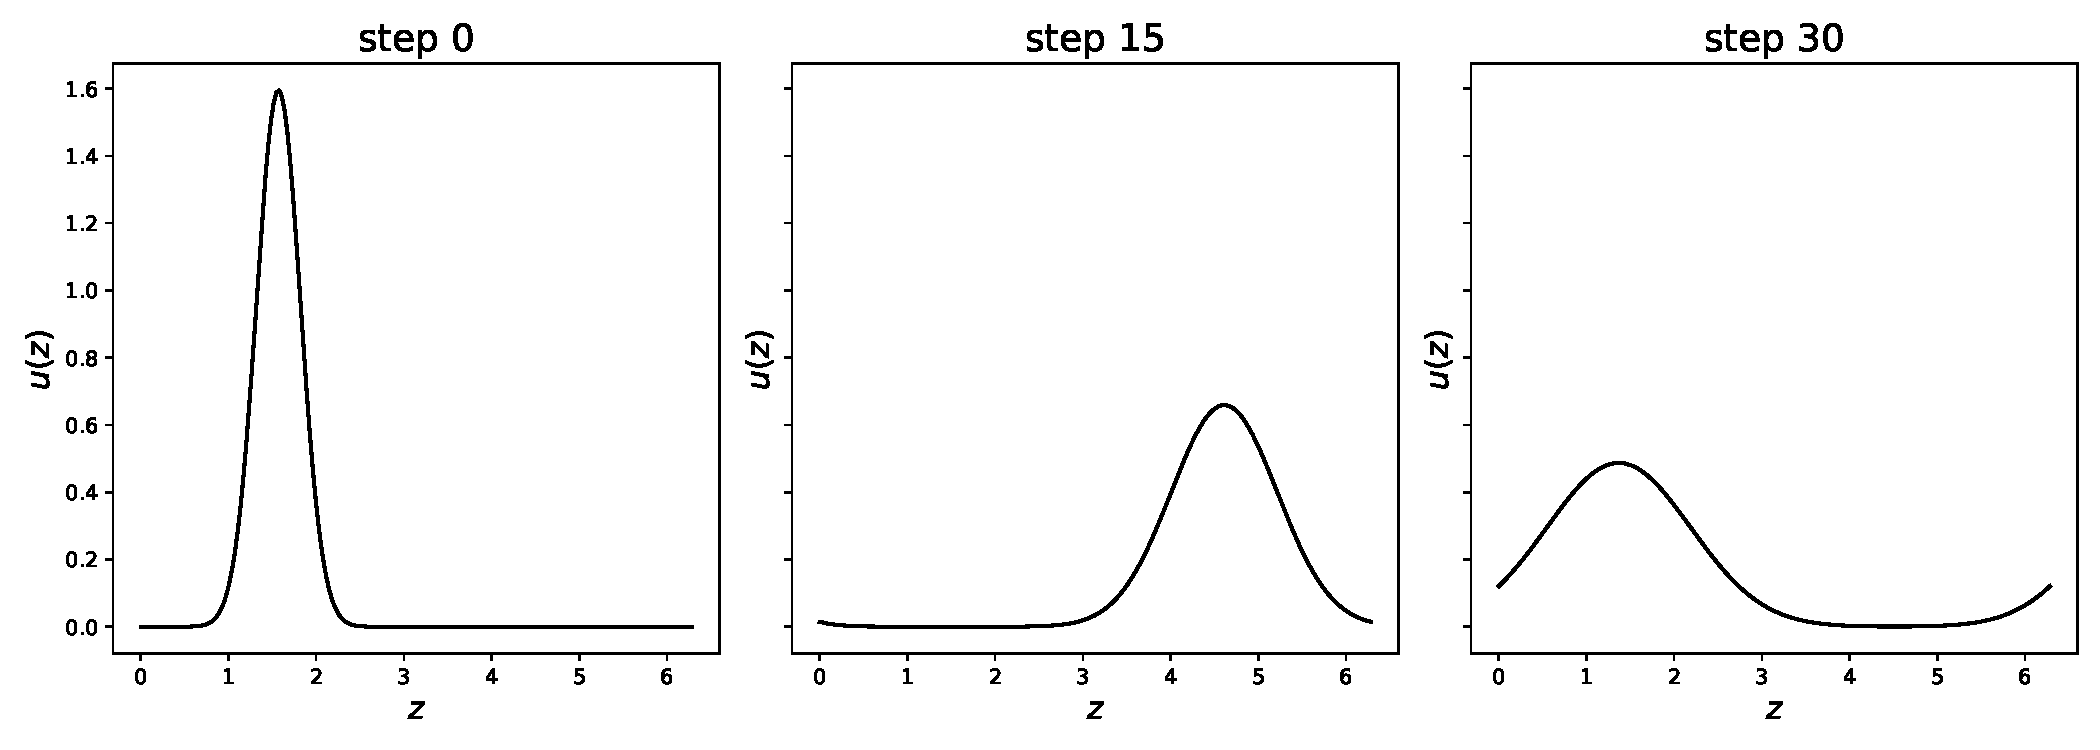
\includegraphics[width=\linewidth]{images/app1d/analytical_frame.pdf}
	\caption{The analytical solution of the convection-diffusion problem evolves over time, with the final snapshot revealing a complete spatial period.}
	\label{fig:1d_analytical}
\end{figure}

Following a Lagrangian perspective by tracking a fluid particle of position $z_p$ and intensity $U_p$, the equation becomes

\begin{equation*}
	\frac{dz_p}{dt} = v(z_p, t), \quad \frac{dU_p}{dt} = D \frac{d^2 U_p}{dz^2}
\end{equation*}

To solve the convection-diffusion scheme, we employ the two steps of the viscous splitting algorithm. The advection is taken into account by updating the position of the particle with an Euler explicit scheme.
On the other hand, we use a redistribution method called the Particle Strength Exchange Method (PSE)~\cite{degond_1989,cottet_1990} to approximate the laplacian term $\frac{d^2 U_p}{dz^2}$.


\begin{equation*}
	D \frac{d^2 U_p}{dz^2}  = D V_p \frac{d^2 u_p}{dz^2} \approx D V_p \varepsilon^{-d} \int [u(z)  - u(y)] \phi_\varepsilon(y - z) dz,
\end{equation*}

It deals with the particle approximation by a redistribution of the particle intensities in their previous locations, such as

\begin{equation*}
	\frac{dU_p}{dt} = D \varepsilon^{-d} V_p \sum_q (U_q - U_p) \phi_\varepsilon( z_q -  z_p),
\end{equation*}where $V_p$ the volume of the particle $p$ and $d$ the dimension of $\Omega$.
For further details on the computation, please refer to \cite{cottet_1990}.

For the periodic boundary problem described in section \ref{App_1D}, we define an equivalent kernel function $\phi_\varepsilon= \phi^P_g = \sum_{n=-\infty}^{+\infty} \phi_g(r - 2 \pi  n )$.

The particle-based model employs a discretization of \npart{} particles with a size of $h = \frac{L}{N_{\text{part}}}$ and a smoothing length of $\varepsilon = 1.3 h$.
For the sake of comparison, we solve the convection-diffusion equation with an explicit central finite difference scheme discretized on a regular grid with \ngrid{} nodes.

\subsection{Assimilation parameters and ensemble generation}

\subsubsection{Ensemble distribution}
All filters undergo testing on an identical initial prior ensemble of size $N = 25$ members, characterized by Gaussian shapes that are shifted and scaled. The mean of the function and its standard deviation are sampled. The total mass is set equal to 1. Parameters of velocity $v$ and the diffusion $D$ are also sampled. The different distributions are defined in Appendix~\ref{tab:ens_gen_1d}. Moreover, the parameters samples and initial state are illustrated in Figure~\ref{fig:initial_gen}.

The observational data is subject to additive noise, denoted as $\eta \sim \mathcal{N}(0, \sigma_y \bm{I})$, where $\sigma_y = \sigmaY$ and $\bm{I}$ represents the identity matrix.

\subsubsection{Error definition}
We define the error as the following relative ratio

\begin{equation}~\label{eq:L2_error}
	e_{L_2} =\frac{ \left[\frac1\nens \sum_{i = 1}^{\nens} \int_\Omega \left(u_i(z) - u^{gt}(z)\right)^2 dz\right]^{1/2}}{\norm{u^{gt}}_{L_2}}
\end{equation}~where $u_i$ denote the $i$-th member of the ensemble and $\norm{u}_{L_2}$ denote the $L_2$ norm of $u^{gt}$.

The $L_2$ norm is computed using a quadrature over a regular grid of an ensemble of cells $\mathcal{C}$ such as for any $f \in L_2$

$$
	\norm{f}_{L_2}  = \int_{\Omega} f^2~d\Omega \approx \sum_{c \in \mathcal{C}} f(z)~V_c
$$~where $z_c$ is the center of the cell $c$ and $V_c$ the volume of the cell. The grid is still the same for all the simulations.
%We compute the parameter error with a norm-2 as $e_{\theta} = \frac{ \left[\frac1\nens \sum_{i = 1}^{\nens} \norm{\theta^{gt} - \theta_{i}}_2^2\right]^{1/2}}{\norm{\theta^{gt}}_2}$.

\subsubsection{Numerical parameters}

We conduct $N_{\text{assim}} = 30$ assimilation steps at evenly spaced intervals until the final time $t_f = 2 \frac{L}{v}$. During each assimilation step, the field $u^{gt}$ is observed at six regularly spaced positions $x_{\text{obs}}$.


In the particle-based simulation, fields are discretized using regularly spaced particles that are shifted. Intensity values are obtained by fitting an interpolation operator like in Section~\ref{interpOp} to the particle intensity.
The parameter $\varepsilon_{\text{mass}}$ is introduced as a cutoff for particle selection, allowing for the definition of varying numbers of particles for each simulation. The particle support poses challenges in the Part-EnKF as described in Section \ref{part_enkf}.

Simultaneously, a standard Ensemble Kalman Filter (EnKF) update is applied to the nodal variables to construct the reference filter Grid-EnKF, which uses a grid-based model. For grid-based simulation, the fields of each member are interpolated at the node locations. In this way, the ensemble generated is still the same for the sake of comparison.


\begin{figure}[ht!]
	\centering
	\begin{subfigure}{0.49\textwidth}
		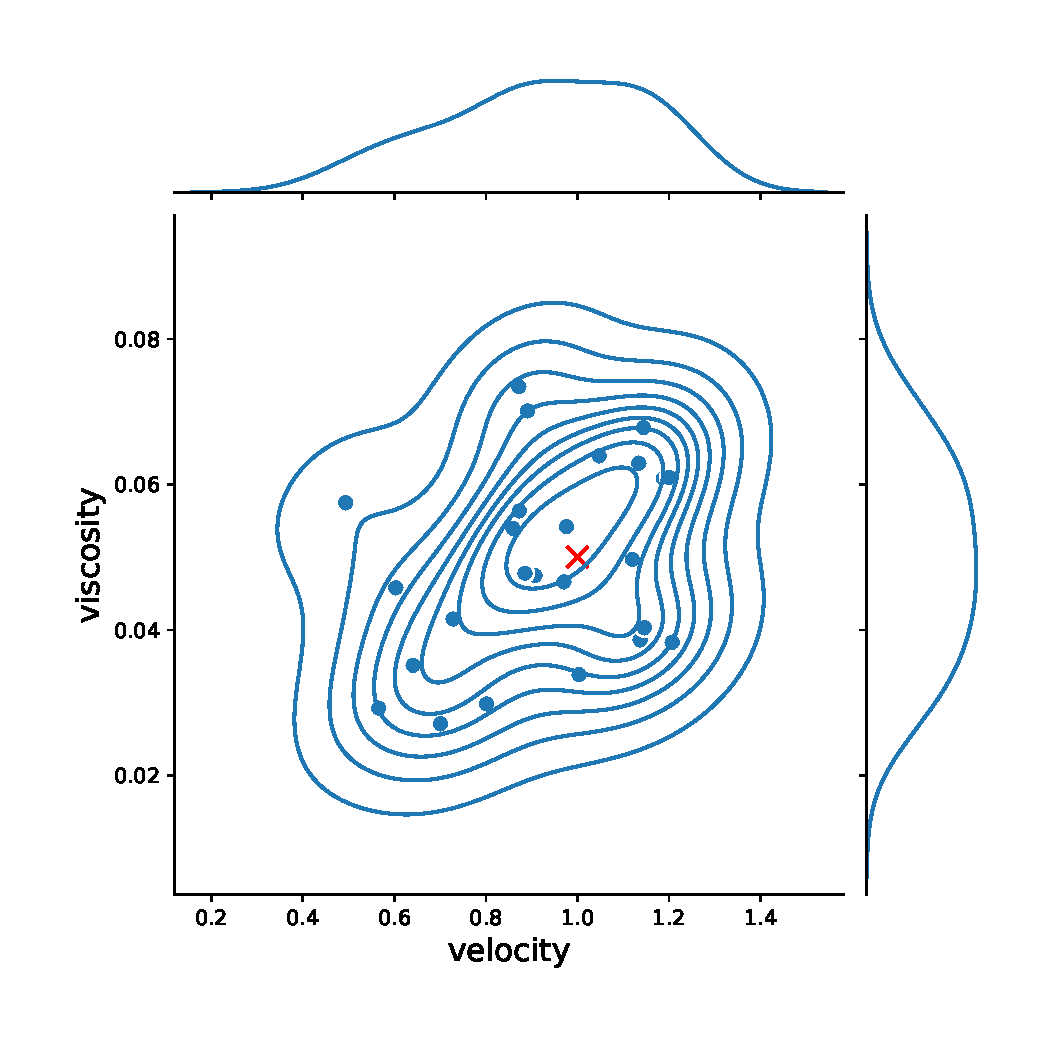
\includegraphics[width=\textwidth]{images/app1d/param.pdf}
	\end{subfigure}
	\hfill
	\begin{subfigure}{0.49\textwidth}
		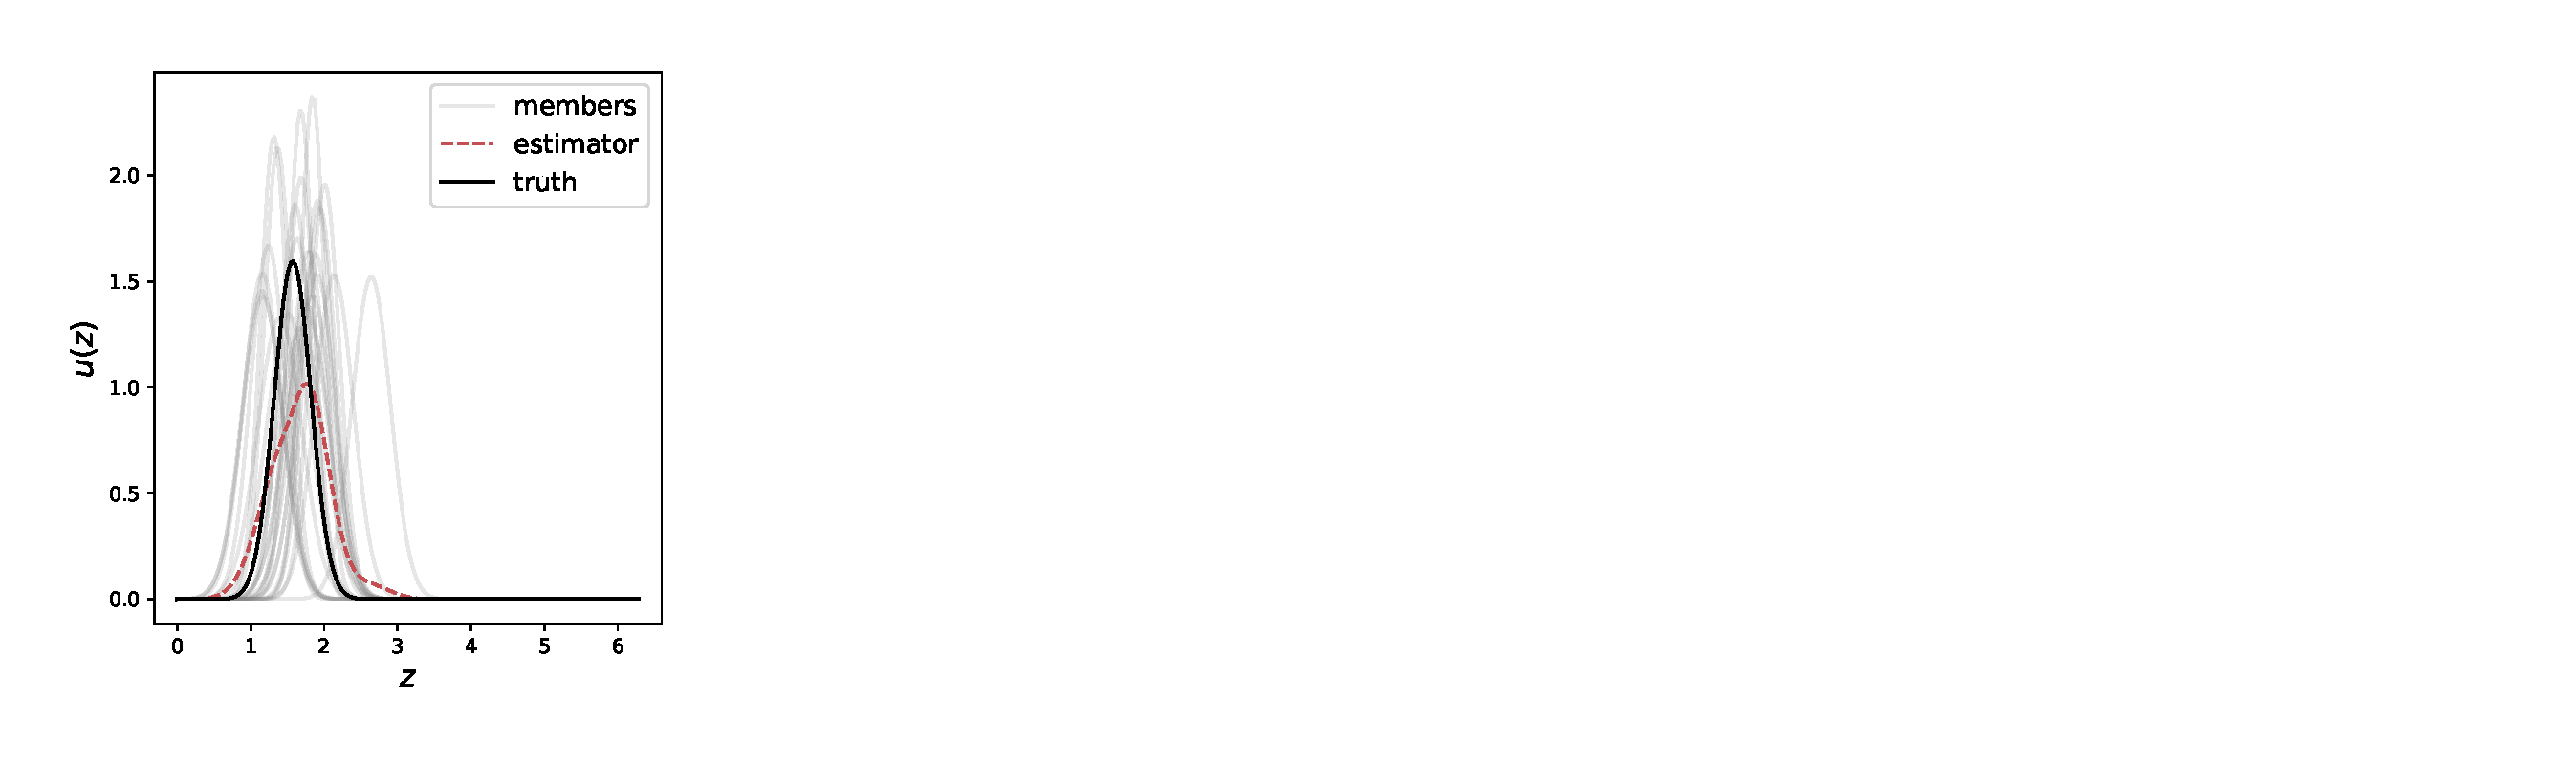
\includegraphics[width=\textwidth]{images/app1d/prior.pdf}
	\end{subfigure}
	\caption{On the left the initial parameters sample, $v$ in abscissa and $D$ in ordinate. On the right is the initial ensemble state.}
	\label{fig:initial_gen}
\end{figure}

\subsection{Results}

We compare the different filters on the assimilation of the state. We first compare the Grid-EnKF, the Remesh EnKF, and two Part-ENKF filters with 100 and 60 particles. The parameter sample is still unchanged. We take unknown parameters into account as model uncertainties. The two filters outlined in the Method section~\ref{Methods} and the Eulerian filter are compared with the reference filter based on a grid discretization.

In figure \ref{fig:1d_error_time}, we appreciate different assimilation steps for the Remesh-EnKF filter.


\begin{figure}
	\centering
	\begin{subfigure}{\textwidth}
		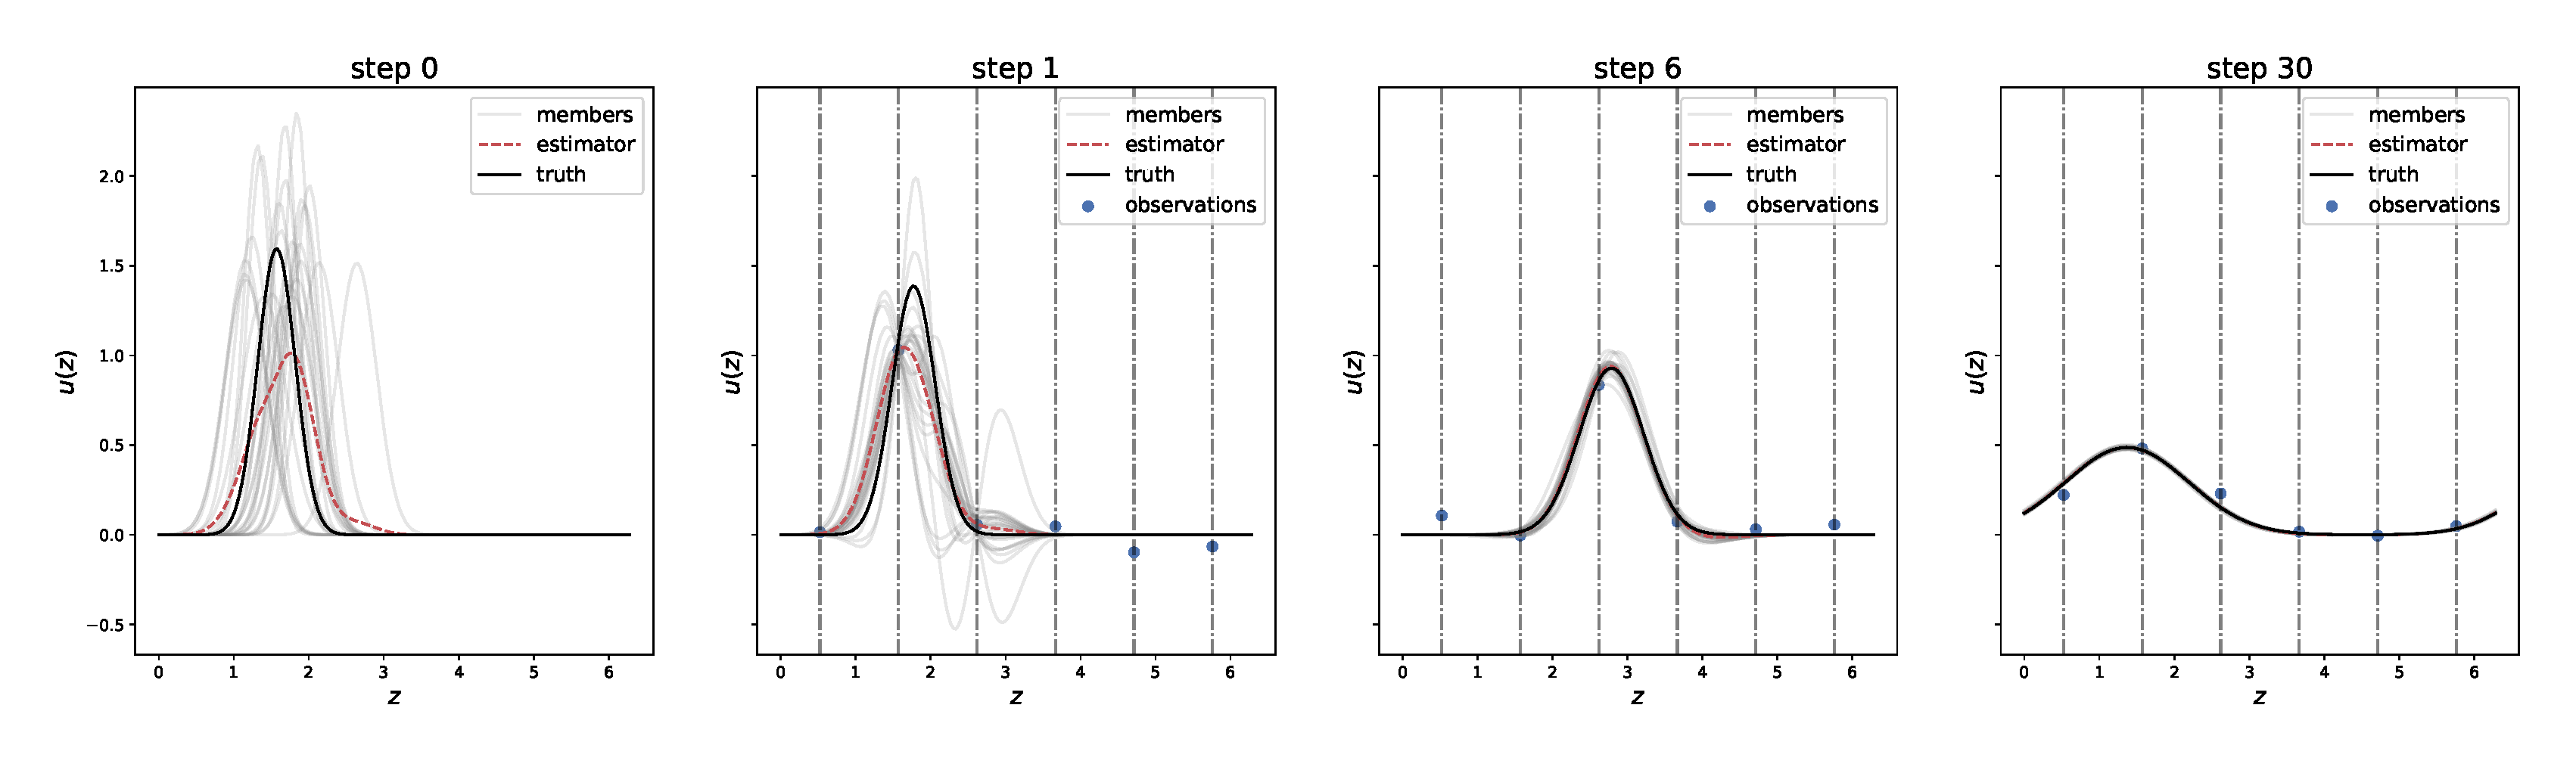
\includegraphics[width=\textwidth]{images/app1d/wo_calibration/remesh_EnKF.pdf}
	\end{subfigure}
	\caption{Data assimilation ower assimilation step for the Remesh-EnKF filter.}
\end{figure}

The result is quite similar for all the different filters except the Part-EnKF with 60 particles.

\begin{figure}
	\centering
	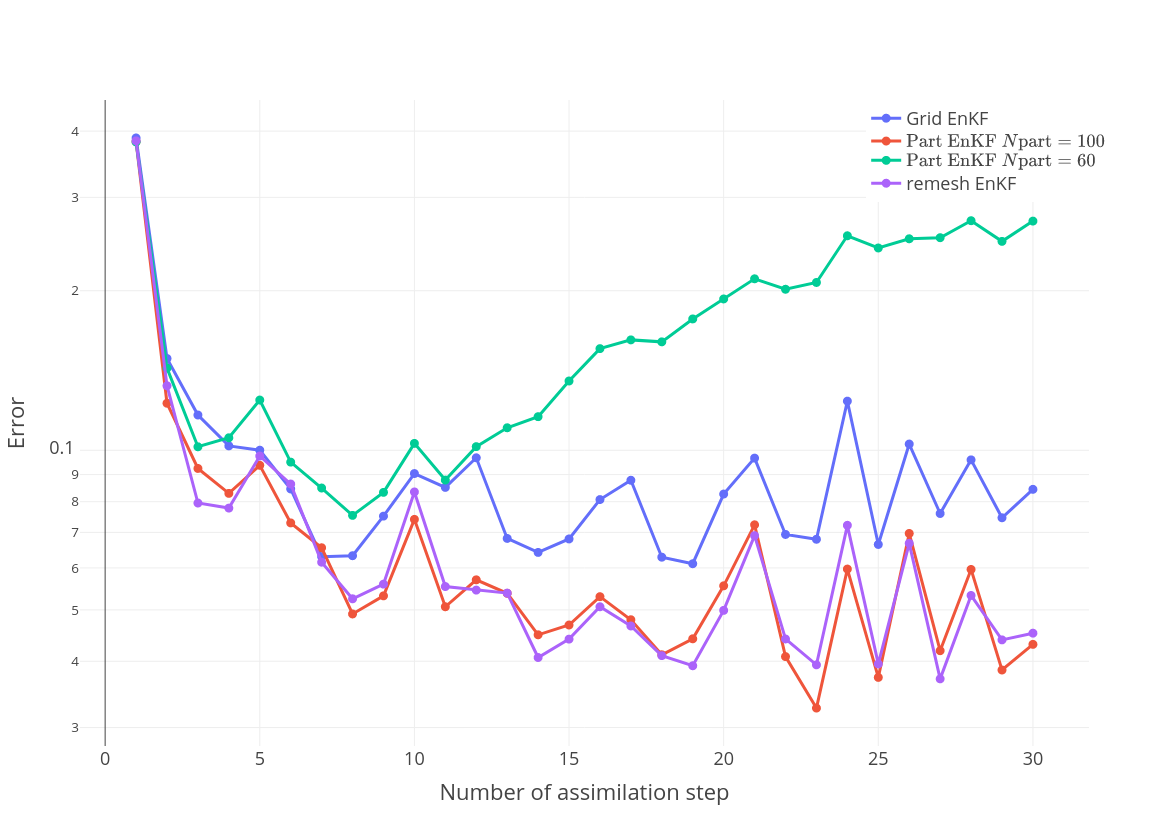
\includegraphics[width=0.75\textwidth]{images/app1d/wo_calibration/state_error.png}
	\caption{State error with respect to assimilation time step.}
	\label{fig:1d_error_time}
\end{figure}

The primary issue arises from the regression on non-overlapping support, where the regression struggles to fit the analysis solution defined on a more considerable space support. This leads to heightened variability, particularly in the tail of the distribution. Addressing this common challenge in RBF Regression \cite{fornberg_flyer_2015} involves increasing the Ridge penalization coefficient, a parameter we choose through cross-validation Ridge regression.
Even with a more stable regression, it remains a projection of the analysis solution onto the forecast support. It is imperative to increase the number of particles to achieve a better approximation of the analysis solution using the particle approximation operator in Section~\ref{interpOp} or the regression operator in Section~\ref{regressionOperator}.

We validate this assumption by varying the initial support of particles. Quantitatively, as observed in Figure~\ref{error_support}, the error estimate and dispersion decrease with an increase in the number of particles. At the level of 70 particles support, a threshold is reached. Moreover, qualitatively examining the snapshot on the right reveals that the solution closely aligns with the reference.

\begin{figure}
	\centering
	\begin{subfigure}{0.39\textwidth}
		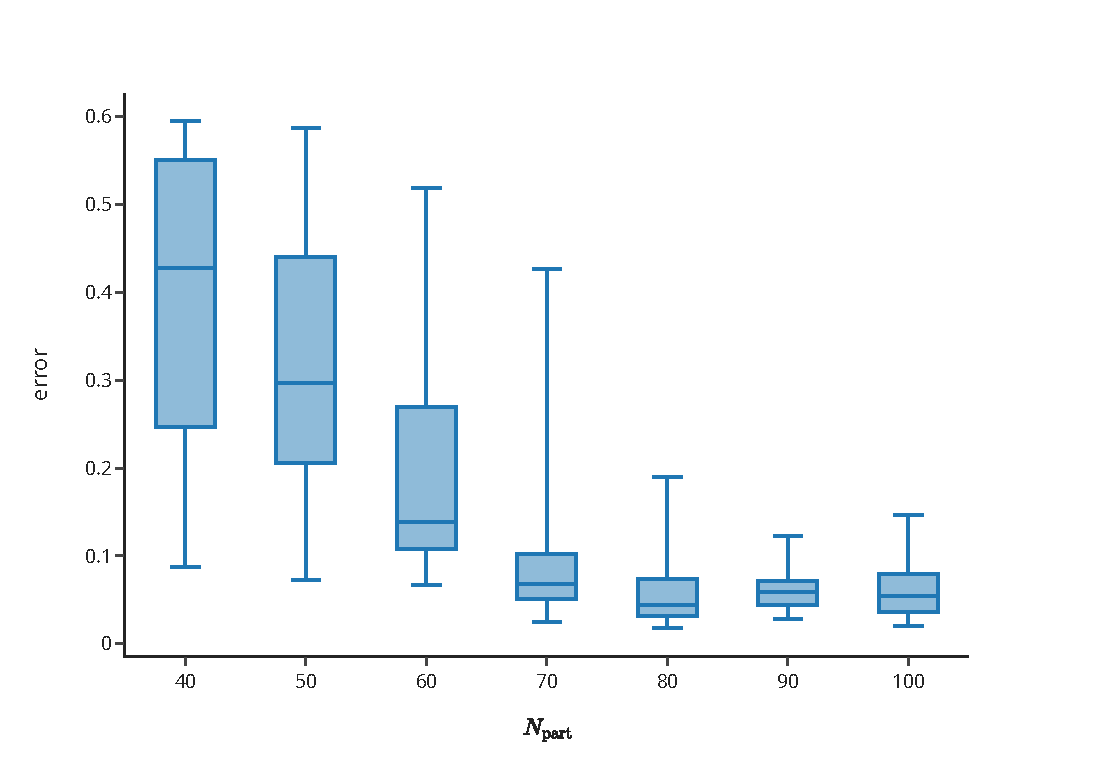
\includegraphics[width=\textwidth]{images/app1d/error_support/error_part.pdf}
		\label{error_support1}
	\end{subfigure}
	\hfill
	% Revoir figures en plotly
	\begin{subfigure}{0.29\textwidth}
		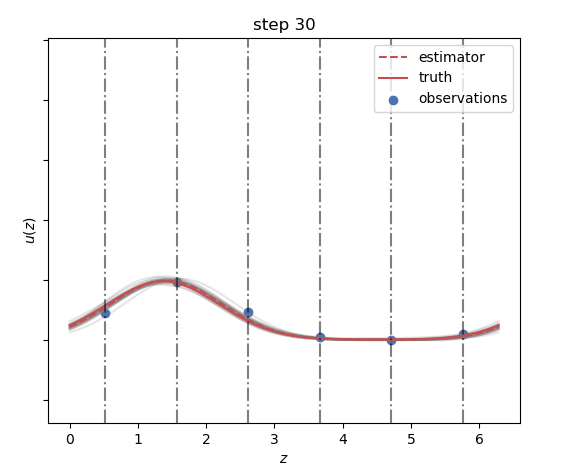
\includegraphics[width=\textwidth]{images/app1d/error_support/ok.png}
		\label{error_support2}
	\end{subfigure}
	\hfill
	\begin{subfigure}{0.29\textwidth}
		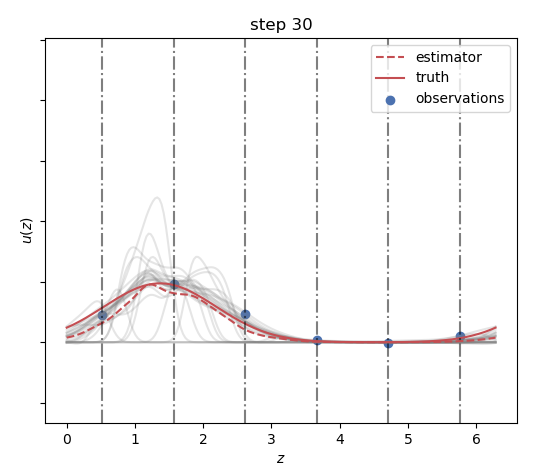
\includegraphics[width=\textwidth]{images/app1d/error_support/not_ok.png}
		\label{error_support3}
	\end{subfigure}
	\caption{Left: Error with respect to particle support size, Middle: Final step for a support of 100 particles, Right: Final step for a support of 60 particles.}
	\label{error_support}
\end{figure}
However, Adding particles to a more complex solution is challenging. Indeed, good spacing between particles and particle density has to be preserved. In this case, we advise defining criteria for the reconstruction' error. Instead of adding particles, we advise generating a new, regularly spaced grid of particles to reconstruct the solution.

In conclusion, this example underscores the Remesh-EnKF filter capability to yield results comparable to the classical EnKF applied to a grid model. Additionally, it highlights the Part-EnKF capability in assimilating on a particle discretization while also emphasizing the importance of addressing spatial discrepancies between members, which can pose challenges in solution reconstruction. The computation of solution error reconstruction provides a straightforward criterion for remeshing a member and applying the analysis solution approximation.


\newpage
% !TEX root = main.tex

\section{2D vortex-in-cell problem}~\label{App_2D}
\subsection{Description of the method}


In this section, we apply the Vortex Method in a two-dimensional scenario, as outlined by Cottet et al. \cite{cottet_vortex_2000}. The Vortex Method is a Lagrangian approach utilizing a particle ensemble to discretize the vorticity field, allowing for the solution of the Navier-Stokes equation for viscous incompressible flow. The method is grounded in the vorticity-velocity formulation of the Euler equation, where $\bm \omega = \nabla \times \bm{v}$ satisfies

\[
	\begin{aligned}
		\frac{\partial \bm \omega}{\partial t} + (\bm{v} \cdot \nabla) \bm \omega - \nu \Delta \bm \omega & = 0, \\
		\nabla \cdot \bm v                                                                                & = 0,
	\end{aligned}
\]where $\omega$ denotes vorticity, $\bm{v}$ represents velocity, and $\nu$ stands for viscosity.

In the context of 2D flow, vorticity is perpendicular to the flow plane, forming a scalar field denoted as $\omega$. In Cartesian coordinates, it is expressed as $\omega = \frac{\partial v_y}{\partial x} - \frac{\partial v_x}{\partial y}$.

The vorticity field is discretized using a collection of discrete vortices, each characterized by a position $\bm z_p$, an associated kernel $\phi_\varepsilon$, and a circulation $\Gamma_p$. For all points $\bm z$ within the domain $\Omega$, the vorticity is expressed as

\begin{equation*}
	\omega(\bm z) = \sum_{i=1}^{N_p} \Gamma_p \phi_\varepsilon(\bm z - \bm z_p).
\end{equation*}

To address the Navier-Stokes equation, we employ a viscous splitting scheme, following the methodology outlined in \cite{cottet_1990}, acknowledging the predominance of the convection term over viscosity. We use the Vortex-In-Cell algorithm \cite{christiansen_1973, birdsall_1969}, coupled with an FFT solver to compute the advection velocity. The subsequent steps involve assigning particle vorticity values to the grid using a particle-to-grid formula and computing the velocity field by solving the Poisson equation on the grid verified by the stream function. Finally, the velocity is interpolated back onto the particles using the grid-to-particles formula. A Runge-Kutta 3 time-stepping scheme is employed to update the particle positions through a time integration scheme. The final phase involves solving the heat equation and updating the particle intensities thanks to the PSE method previously described in Section~\ref{App_1D}.

\subsection{Lamb-Chaplygin dipole and simulation parameters}

We define the reference as the advection of the Lamb-Chaplygin dipole inside a close domain with stress-free walls. Lamb-Chaplygin dipole is a popular choice for numerical studies \cite{orlandi_vortex_1990}. The model represents a specific steady, inviscid dipolar vortex flow and offers a non-trivial solution to the two-dimensional Euler equations. The dipole is characterized by a translation velocity $U$, a mean position $\bm{z}_0$, a radius $R$, and an orientation $\alpha$.

The dipole vorticity field $\omega$ could be expressed as

\begin{equation*}
	\omega(r) = \begin{cases}
		\frac{-2 k U J_1(kr)}{J_0(kR)} \sin \alpha \quad & \text{for} \quad  r < R, \\
		0 \quad                                          & \text{otherwise},
	\end{cases}
\end{equation*}where $(r, \alpha)$ represent the polar coordinates in the dipole reference frame. Here, $J_0$ and $J_1$ denote the zeroth and first-order Bessel functions of the first kind, respectively, and $k$ is determined such that $kR$ corresponds to the first non-trivial zero of the first Bessel function. The dipole vorticity field is depicted in Figure \ref{fig:lamb_dipole}.

\begin{figure}[ht]
	\centering
	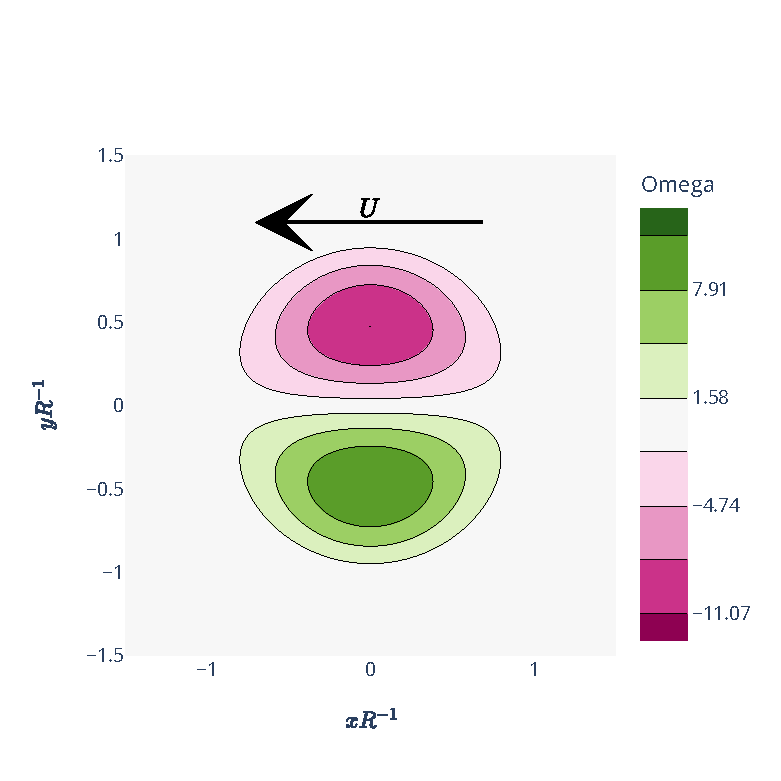
\includegraphics[width=0.6\linewidth]{images/app2d/lamb.pdf}
	\caption{The Lamb-Chaplygin dipole vorticity field on a normalized space.}
	\label{fig:lamb_dipole}
\end{figure}

The dipole is positioned at the center of a box with dimensions $[0, \pi] \times [0, \pi]$, featuring an orientation of $\frac{7\pi}{8}$ rad., a radius of $0.5$ meters, and a velocity $U$ of $0.25 \text{ m.s}^{-1}$. The complete reference setting is listed in Table \ref{tab:ref}.

The boundary box features stress-free walls, meaning fluid cannot pass through them. The velocity perpendicular to the walls is zero, while tangential velocity remains undetermined. When a vortex, such as a dipole, reaches this boundary, it walks along the wall, sensing its reflection and interacting with it.

Because this problem does not have an explicit solution on a closed domain, we simulate the ground truth with the vortex method for a fined discretization and fixed set of parameters also described in Table \ref{tab:ref}. The trajectory of the ground truth is illustrated in Figure \ref{fig:ref_trajectory} on a regularly spaced grid.

\begin{figure}[htbp]
	\begin{subfigure}{0.32\textwidth}
		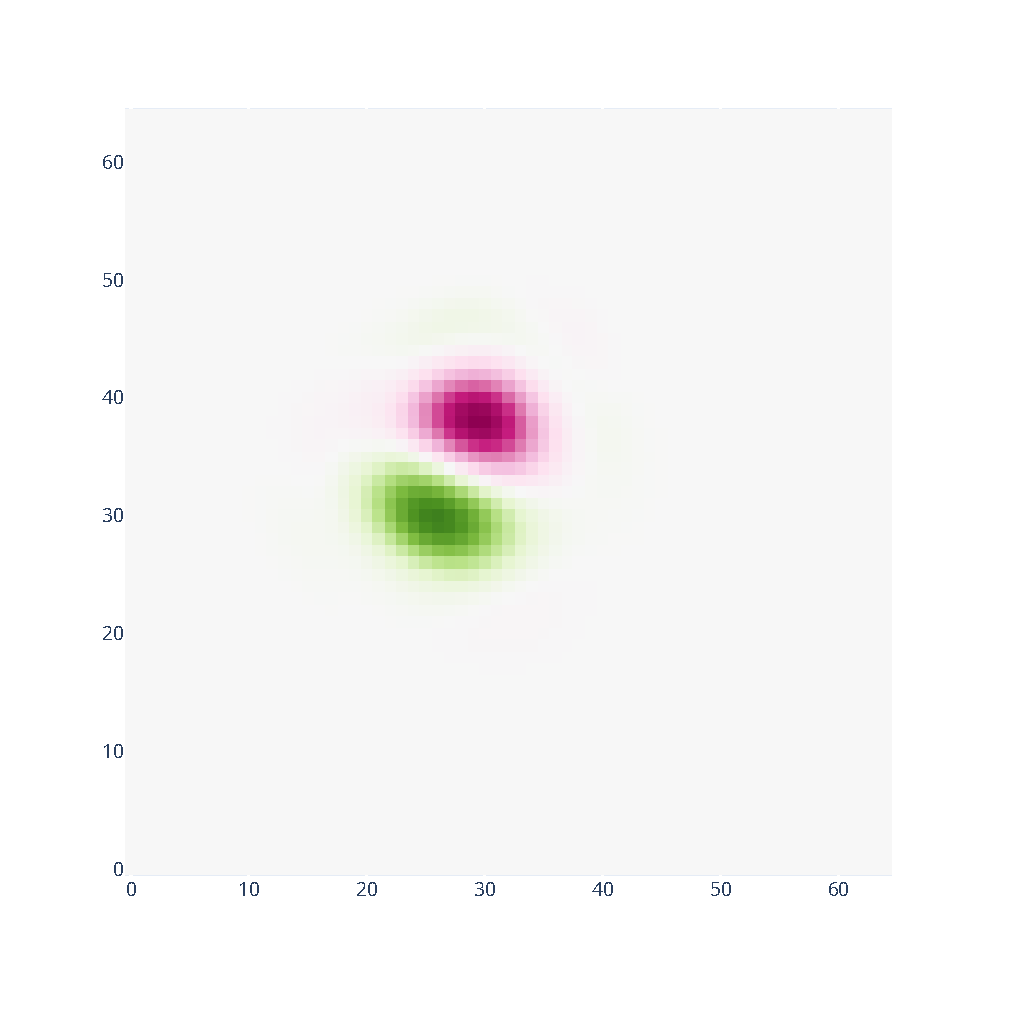
\includegraphics[width=\linewidth]{images/app2d/best_estimate_2.pdf}
	\end{subfigure}
	\hfill
	\begin{subfigure}{0.32\textwidth}
		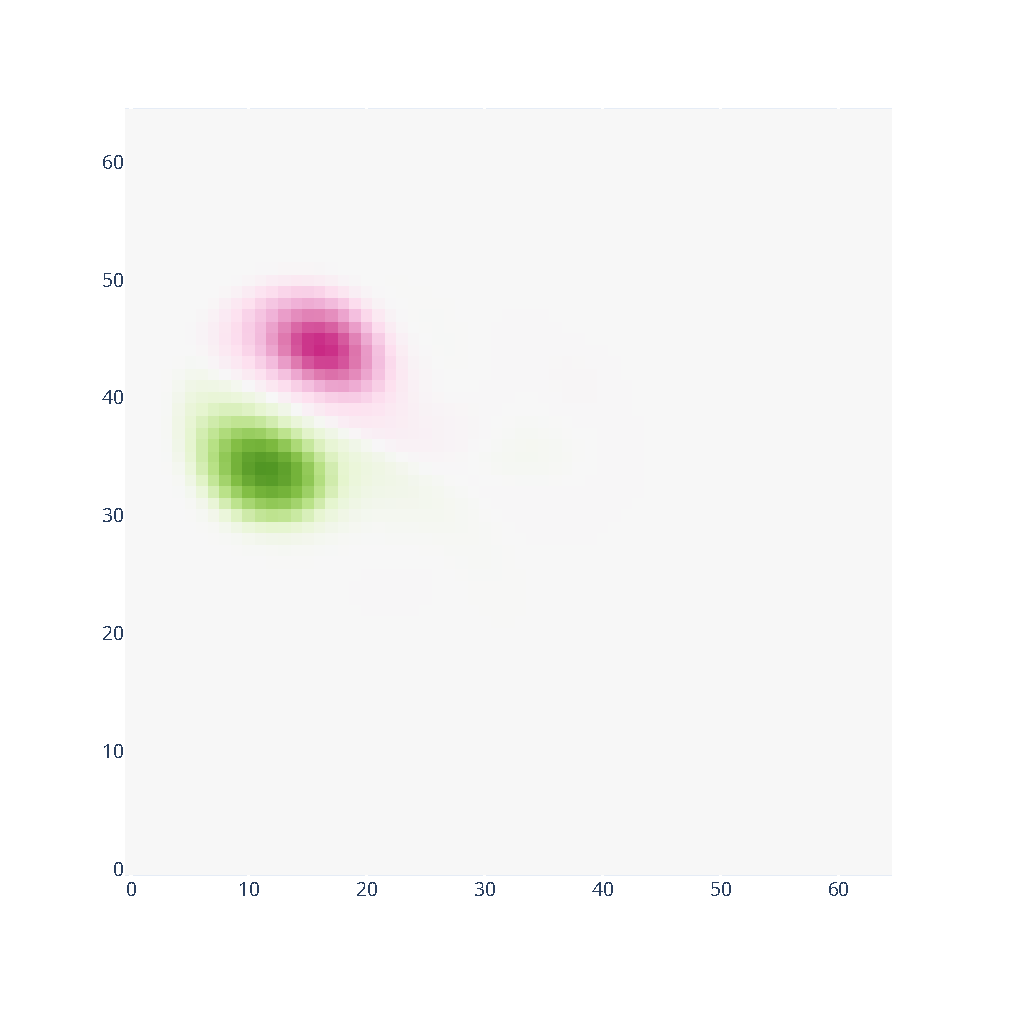
\includegraphics[width=\linewidth]{images/app2d/best_estimate_10.pdf}
	\end{subfigure}
	\hfill
	\begin{subfigure}{0.32\textwidth}
		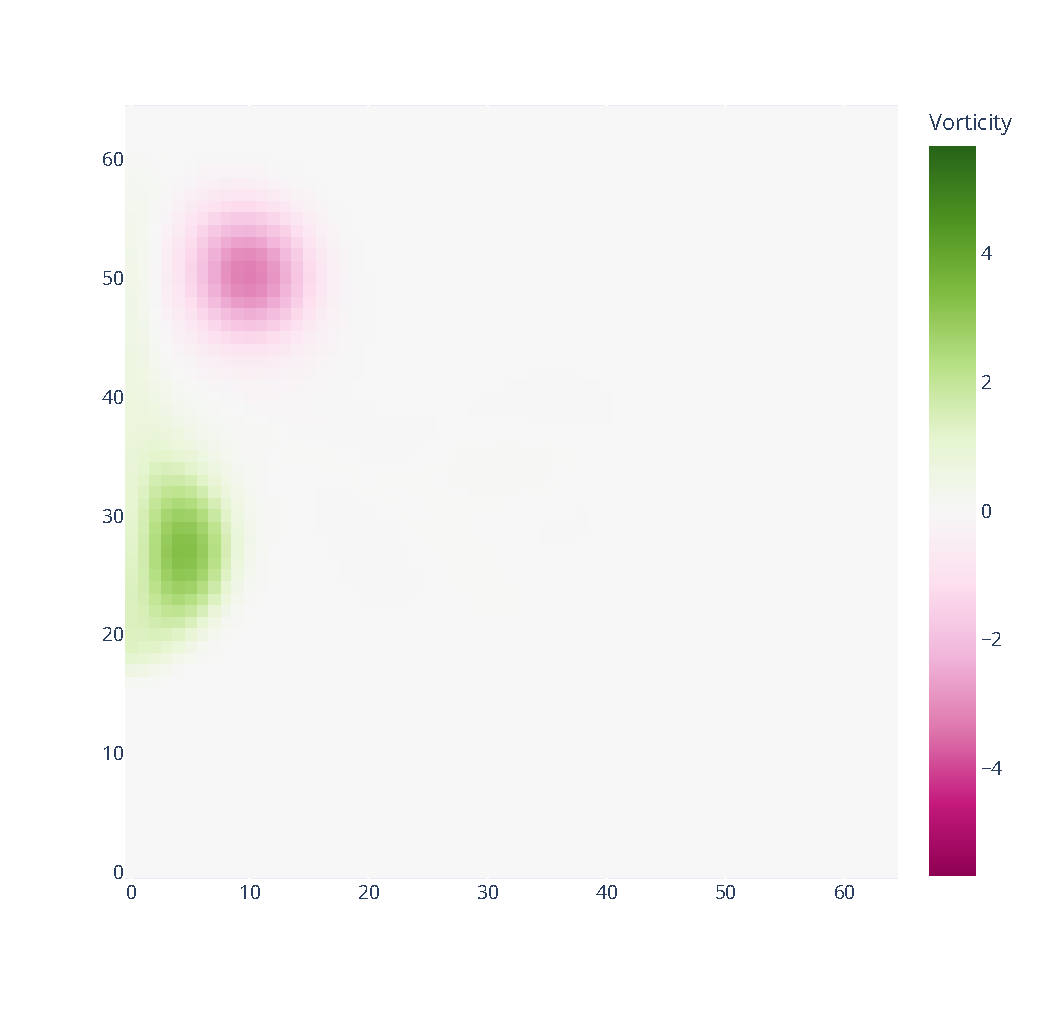
\includegraphics[width=\linewidth]{images/app2d/best_estimate_20.pdf}
	\end{subfigure}
	\caption{Trajectory of the ground truth. The vorticity is represented on a regularly spaced grid. For $t=[1, 5, 10]s.$}
	\label{fig:ref_trajectory}
\end{figure}
Several parameters in the simulation influence the particle distribution and can lead to different results. The first one is the particle size defined by $d_p$. Another significant parameter is $\varepsilon_\omega$, associated with the remeshing process occurring either during the forecast (to prevent high distortion of the particle distribution) or during the Remesh-EnKF filter. $\varepsilon_\omega$ serves as a threshold, determining whether a particle is retained after the remeshing process based on the condition $V_p \Gamma_p > \varepsilon_\omega$. The impact of this parameter is illustrated for one member after the first forward in Figure~\ref{fig:eps_effect}.

\begin{figure}[htbp]
	\centering
	\begin{subfigure}{0.3\textwidth}
		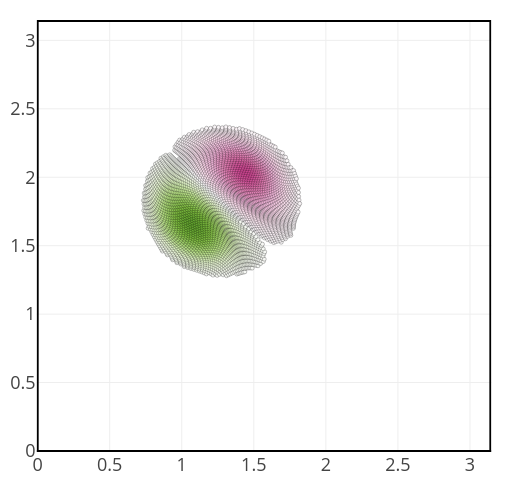
\includegraphics[width=\linewidth]{images/app2d/part_eps_0.1.png}
	\end{subfigure}
	\hfill
	\begin{subfigure}{0.3\textwidth}
		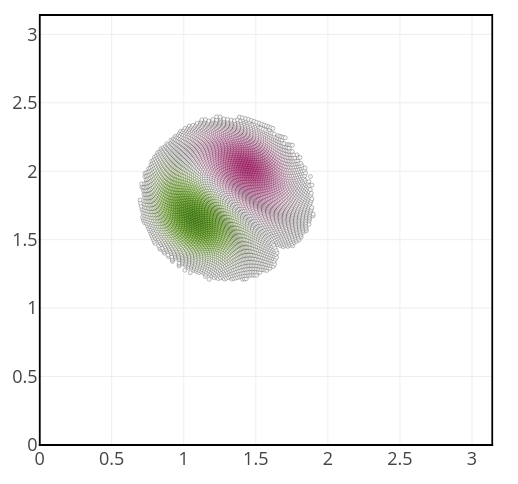
\includegraphics[width=\linewidth]{images/app2d/part_eps_0.01.png}
	\end{subfigure}
	\hfill
	\begin{subfigure}{0.3\textwidth}
		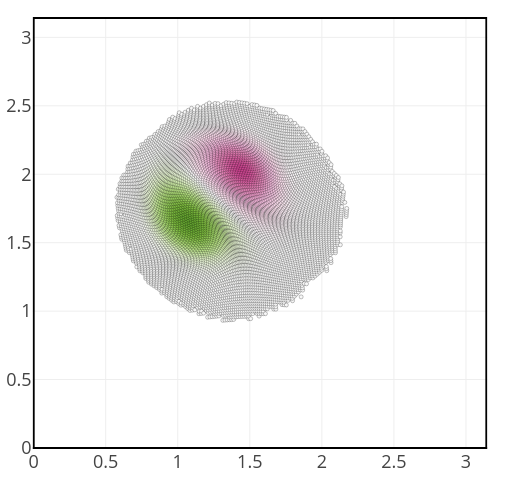
\includegraphics[width=\linewidth]{images/app2d/part_eps_1e-6.png}
	\end{subfigure}
	\caption{Effect of the parameter $\varepsilon_\omega$ on the particle discretization of the solution for one member. From left to right, results for $\varepsilon_\omega = 0.1, 0.01$, and $1.e^{-6}$.}
	\label{fig:eps_effect}
\end{figure}

For the following paragraphs, if the value is not explicitly changed, we use the nominal parameters described in Table \ref{tab:simu_2d} for the simulation.

\subsection{Assimilation parameters and ensemble generation}

\subsubsection{Ensemble distribution}
An ensemble of 32 members is created by sampling distributions over the dipole parameters. We sample the radius $R$, the prescribed velocity $U$, the orientation $\alpha$, and the barycenter $\bm z_{\text{mean}}$. Additionally, the model viscosity $\nu$ is also sampled. All the distributions are summarized in Table \ref{tab:ens_dipole}. The first six members are plotted in Figure \ref{fig:sample_ens}.

\begin{figure}[ht]
	\centering
	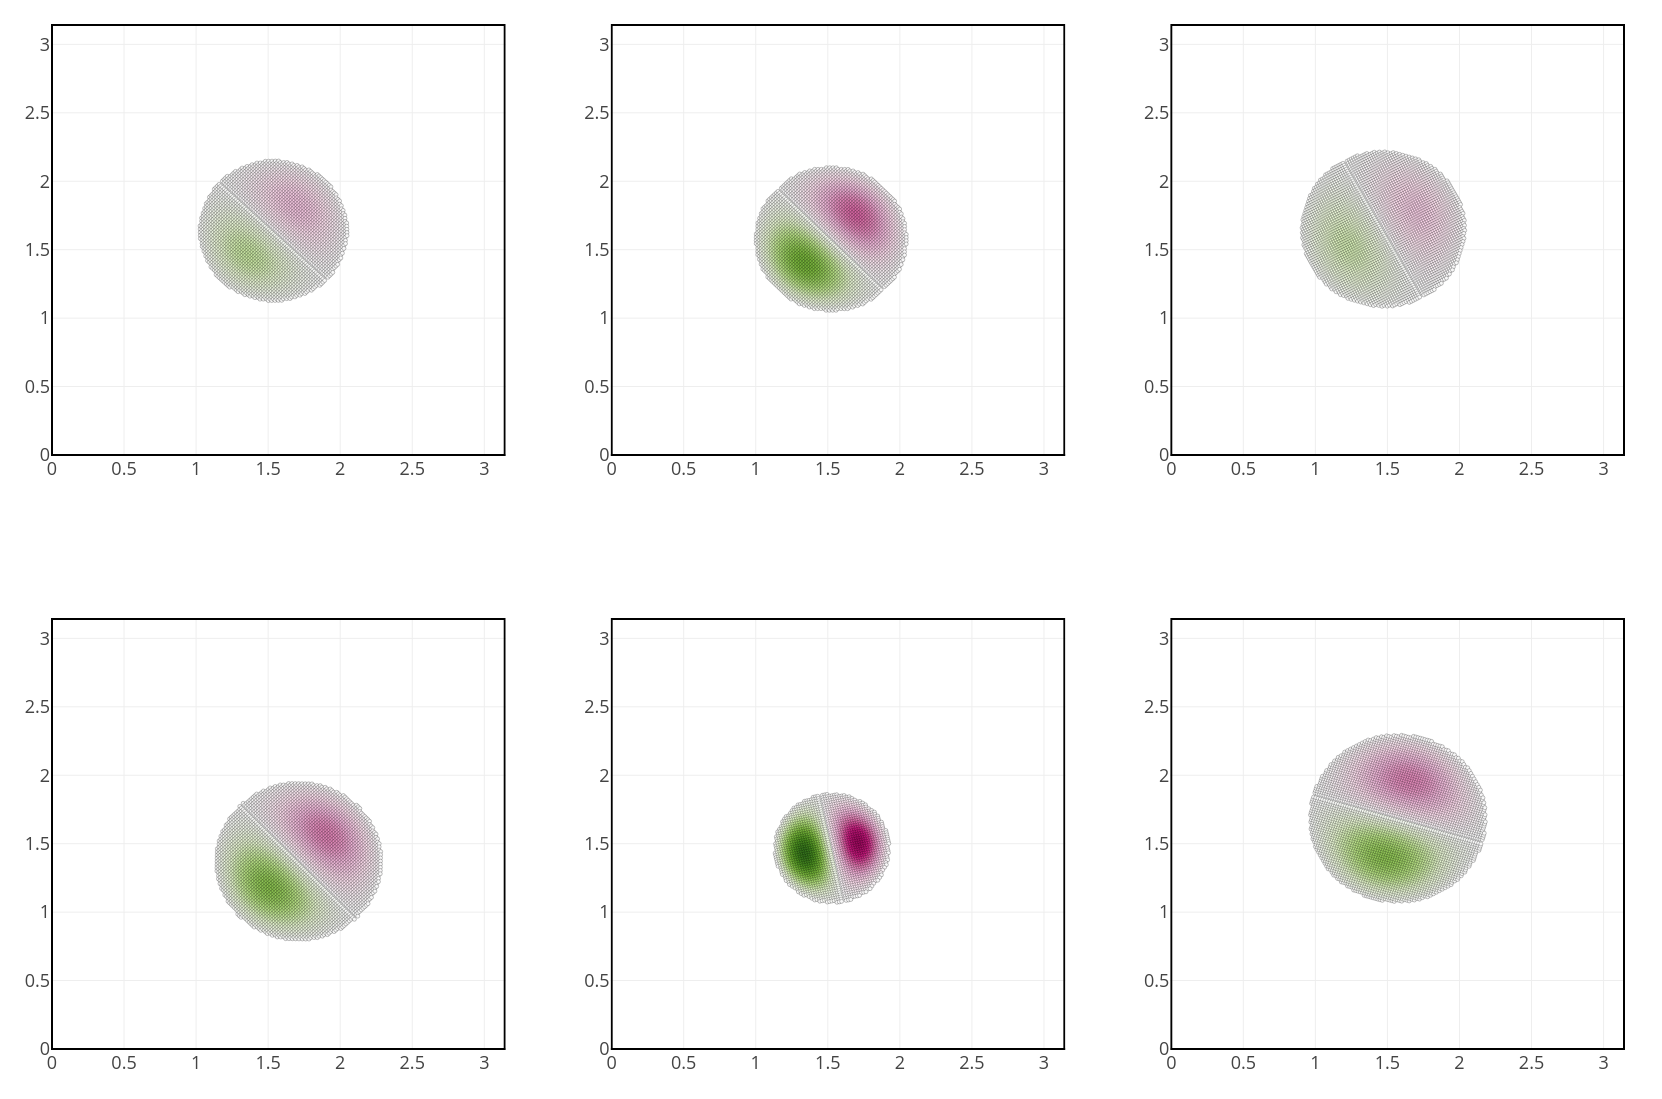
\includegraphics[width=0.9\linewidth]{images/app2d/ensemble_sample.png}
	\caption{Six samples from the initial ensemble.}
	\label{fig:sample_ens}
\end{figure}

The initial vorticity field is first discretized on a regular grid of particles with a characteristic length $d_p$, where each particle receives the circulation $\Gamma_p = \omega(\bm z_p) V_p$ and $V_p = d_p^2$ represents the volume of the particle.

\subsubsection{Error definition}

We use an absolute error absolute \(L_2\)-error defined as $ \frac1\nens \sum_{i = 1}^{\nens} \int_\Omega \left(\omega_i(\z) - \omega^{gt}(\z)\right)^2 \mathrm{d}\z$.
We also use the member errors to evaluate the dispersion of the error estimate.

\subsubsection{Numerical parameters}

The assimilation frequency is defined by the assimilation step $dt_a$. The simulation is performed over a duration of $t_f$. All simulation parameters are summarized in Table \ref{tab:simu_2d}.

Observations are collected on a regular grid of size $N_{\text{obs}}$, measuring both components of the velocity. The observations follow a normal distribution $\mathcal N(0, \sigma_{\text{obs}}^2 \bm{I})$, indicating an ensemble of independent measurements, each characterized by a standard distribution of $\sigma_{\text{obs}}$. An example of observed velocity with and without noise is illustrated in Figure \ref{fig:velocity}.

\begin{figure}[htbp]
	\centering
	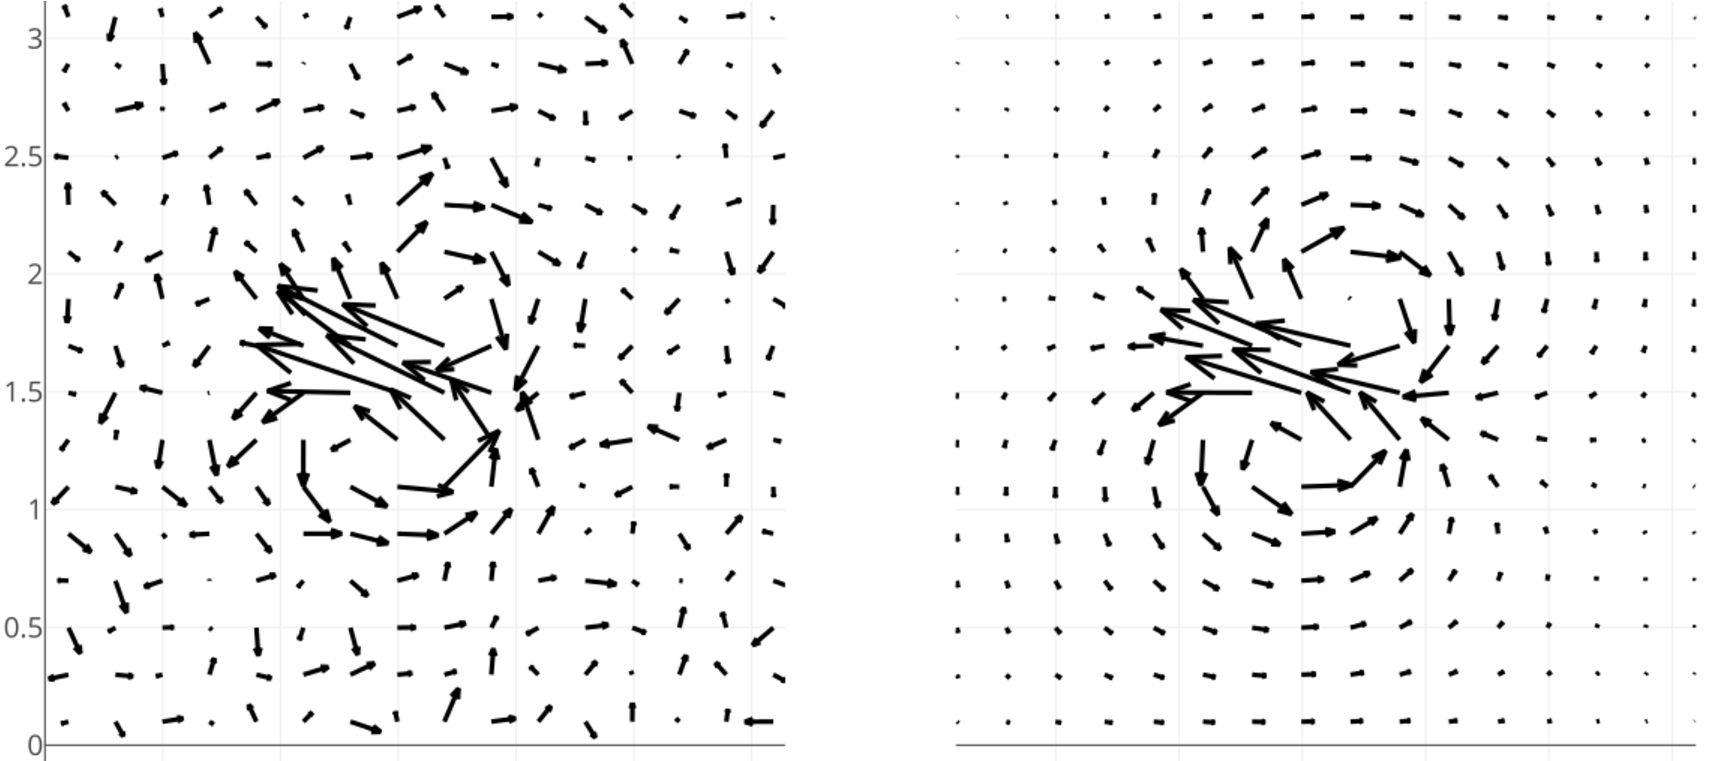
\includegraphics[width=0.8\linewidth]{images/app2d/velocity_ref_recadre.pdf}
	\caption{Observed and reference velocity fields. The error on each component is a sample from a centered normal distribution with the nominal value $\sigma_{\text{obs}} = 0.05$.}
	\label{fig:velocity}
\end{figure}

\newpage

\subsection{Results}

\subsubsection{Error through time}

We start by analyzing the assimilation error over time. Figure \ref{fig:assim_time} illustrates the error throughout the assimilation process for the nominal set of assimilation parameters, demonstrating comparable results for both filters. At each assimilation step, the error decreases and prevents the solution from diverging elsewhere.

\begin{figure}[htbp]
	\centering
	\includegraphics*[width=0.7\linewidth]{images/app2d/final/error_in_time.pdf}
	\caption{error curves through assimilation steps. Left: \(L_2\)-error of the field, Right: Error for the viscosity parameter. With Part-EnKF in blue and Remesh-EnKF in red.}
	\label{fig:assim_time}
\end{figure}

\newpage

\subsubsection{Error with respect to assimilation parameters}
We also assess the performances of the different filters by evaluating the convergence of the error with respect to the assimilation parameters.

We observe the convergence rate concerning data assimilation parameters: The observation precision, which is \(1/\sigma_{\text{obs}}^2\), the number of observations \(N_{\text{obs}}\), the number of assimilation step \(N_{\text{assim}}\).

Figure \ref{fig:obs_precision_1} illustrates a decreasing error bias and variances with respect to observation precision similarly for both filters. What is striking in the same Figure~\ref{fig:obs_precision_2} but in the log-scale is the regular convergence rate for both filters with respect to the observation precision. The order of convergence is about 0.68 for Part-EnKF and 0.75 for Remesh-EnKF.

\begin{figure}[h!]
	\centering
	\begin{subfigure}{0.49\linewidth}
		\centering
		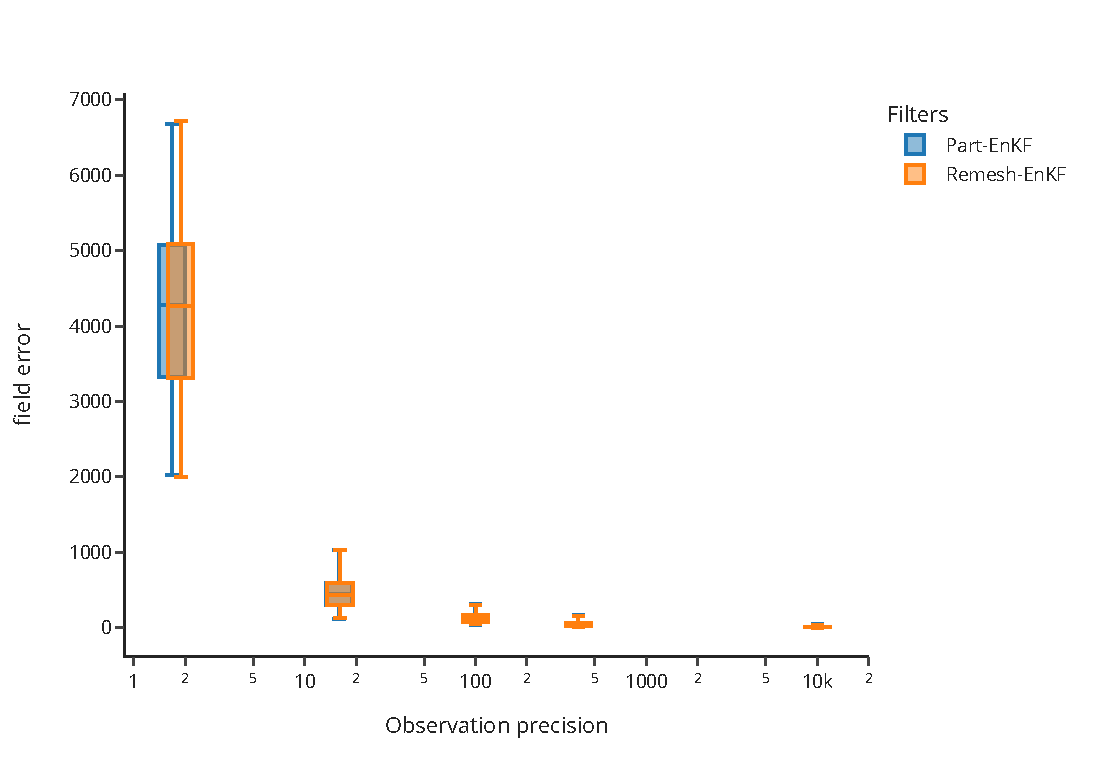
\includegraphics[width=\linewidth]{./images/app2d/final/MSE_obs_precision_box.pdf}
		\caption{}
		\label{fig:obs_precision_1}
	\end{subfigure}
	\begin{subfigure}{0.49\linewidth}
		\centering
		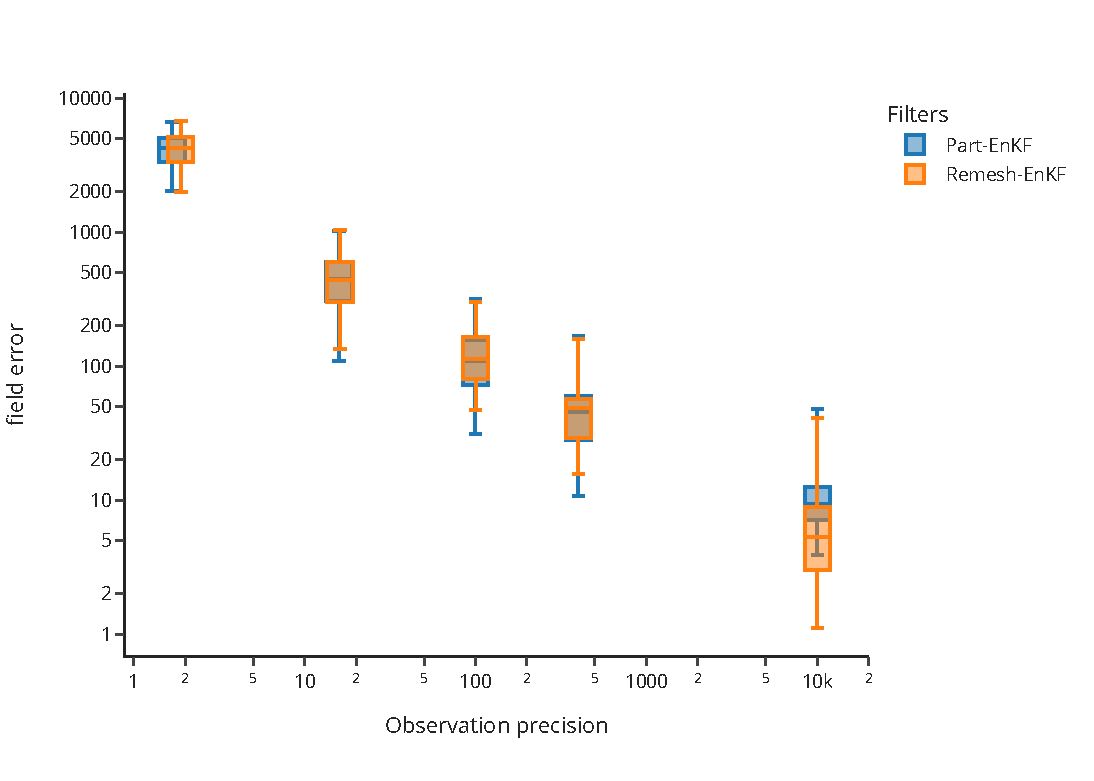
\includegraphics[width=\linewidth]{./images/app2d/final/MSE_obs_precision_box_log.pdf}
		\caption{}
		\label{fig:obs_precision_2}
	\end{subfigure}
	\caption{Box plots of the state error w.r.t. $1/\sigma_{\text{obs}}^2$.}
\end{figure}


In Figure~\ref{fig:na_1}, the reduction of error is still prominent and shows a reduction of variance as the number of observations increases. In the log-scale Figure~\ref{fig:na_2}, the error decrease also at a constant rate for both filters. We notice a more substantial order of 1.8 for the Remesh-EnKF compared to an order of 1.4 for Part-EnKF.

\begin{figure}[h!]
	\centering
	\begin{subfigure}{0.49\linewidth}
		\centering
		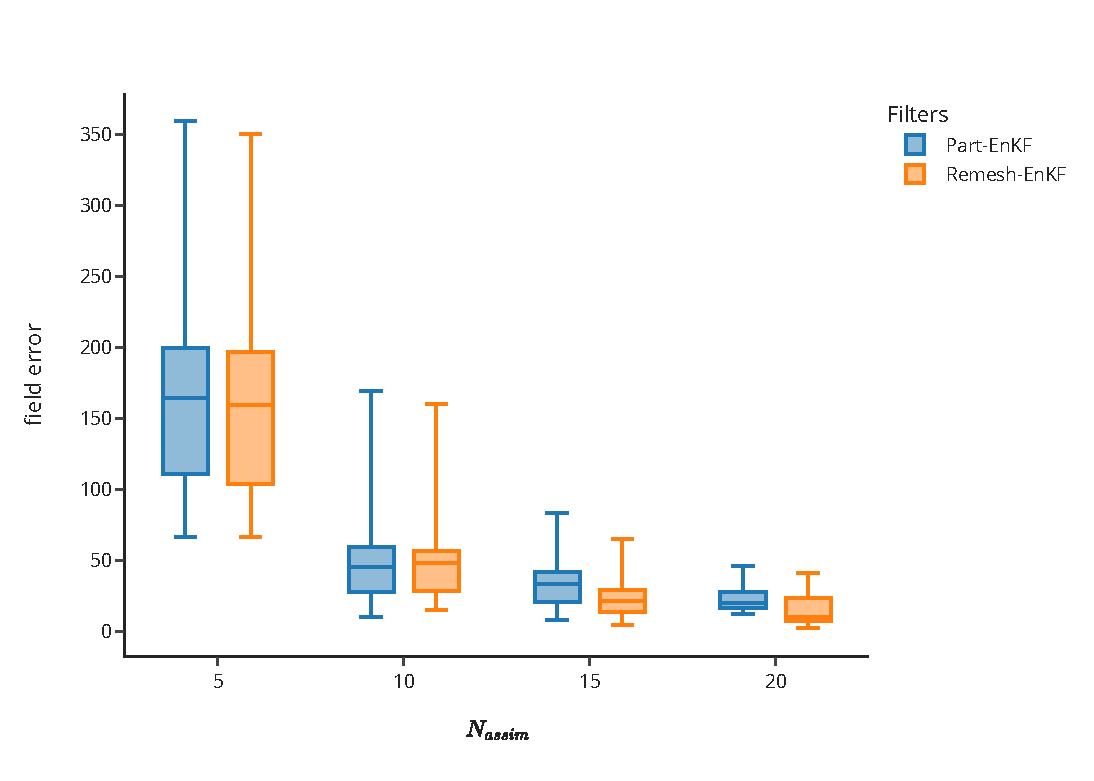
\includegraphics[width=\linewidth]{./images/app2d/final/MSE_na_box.pdf}
		\caption{}
		\label{fig:na_1}

	\end{subfigure}
	\begin{subfigure}{0.49\linewidth}
		\centering
		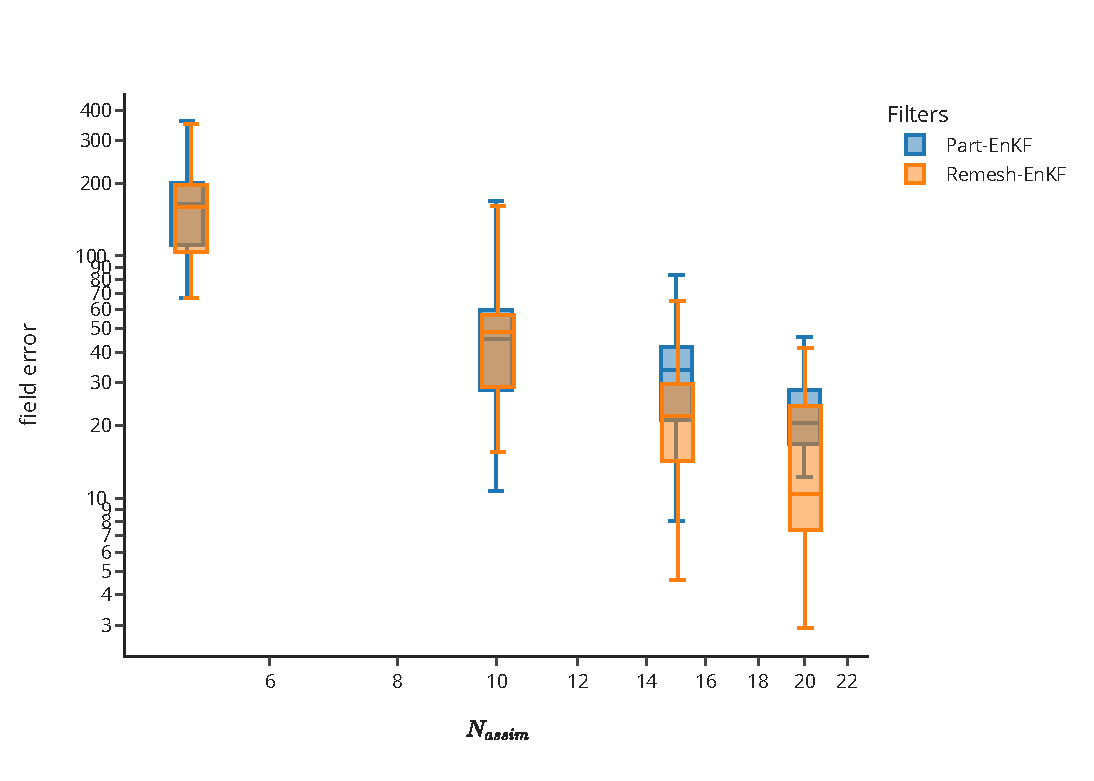
\includegraphics[width=\linewidth]{./images/app2d/final/MSE_na_box_log_log.pdf}
		\caption{}
		\label{fig:na_2}
	\end{subfigure}
	\caption{Box plots of the state error w.r.t. $N_{\text{assim}}$.}
	\label{fig:na}

\end{figure}

Finally, we analyze the error convergence with respect to the number of observations. Observation locations increase regularly on both axes. In Figure~\ref{fig:nobs_1}, the error estimate and variances decrease. For a relatively small number of observations, the two filters offer similar results when, in contrast, the Remesh-EnKF has relatively better results when the number of observations is increased. Moreover, the convergence rate seems to change around 200 observation points, as illustrated in the log-scale Figure~\ref{fig:nobs_2}. Nevertheless, it illustrates adequate performances for both filters.

\begin{figure}[h!]
	\centering
	\begin{subfigure}{0.49\linewidth}
		\centering
		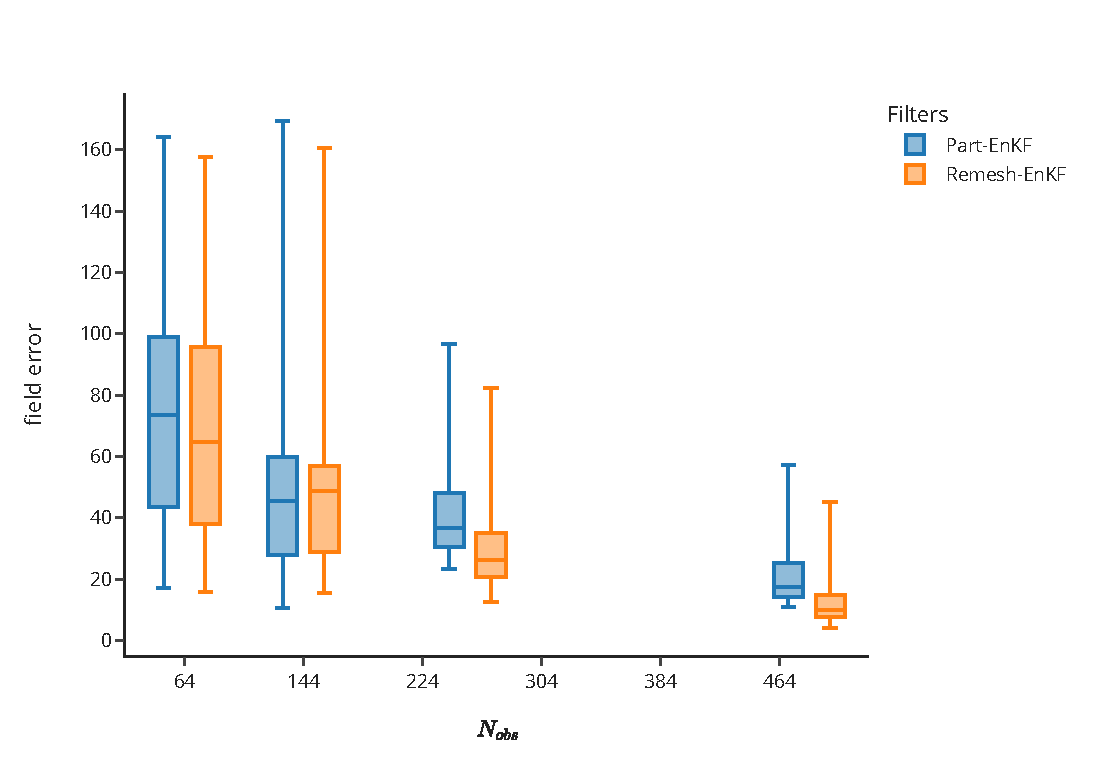
\includegraphics[width=\linewidth]{./images/app2d/final/MSE_nobs_box.pdf}
		\caption{Box plots of the state error w.r.t. $N_{\text{obs}}$.}
		\label{fig:nobs_1}
	\end{subfigure}
	\begin{subfigure}{0.49\linewidth}
		\centering
		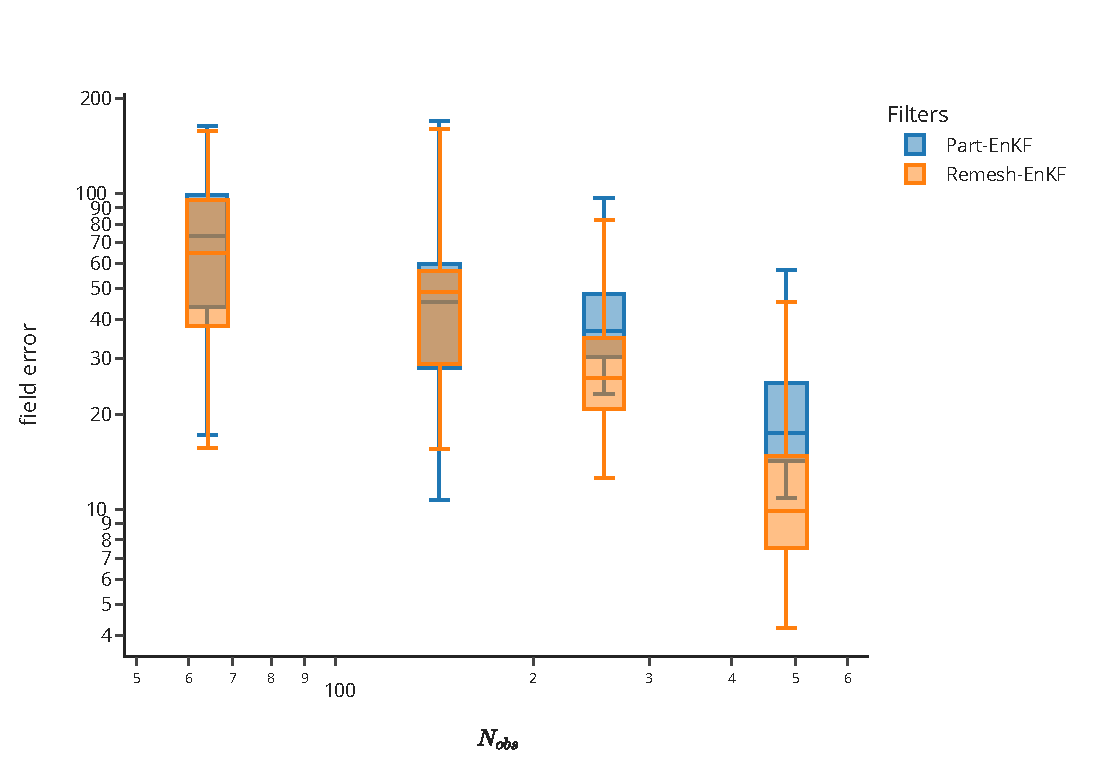
\includegraphics[width=\linewidth]{./images/app2d/final/MSE_nobs_box_log_log.pdf}
		\caption{Box plots of the state error w.r.t. $N_{\text{obs}}$.}
		\label{fig:nobs_2}
	\end{subfigure}
	\label{fig:nobs}

	\label{fig:assim_params}
\end{figure}



\subsubsection{Error with respect to simulation parameters}

To better understand the differences, let us now turn to the evolution of the error with respect to particle discretization parameters. For the Part-EnKF, remember that each member has its own particle discretization that flows according to the dipole direction and velocity. Each analyzed member's solutions are then respectively projected on their member discretization. However, this scheme could introduce different sources of error. First, due to particle irregularity in the particle distribution, severe approximation was introduced, which led to errors between the analyzed and the approximated solution. Even more seriously, certain parts of the solution may vanish as no particle in the support can interpolate it. This effect could be appreciated on several samples of the ensemble where the analysis is projected on a non-conforming particle discretization. For instance, we analyzed the first assimilation step of one member for the different filters. If the analyzed field is known over the space domain, we observed in Figure~\ref{fig:assim_member} that the Remesh-Filter and Part-Grid-EnKF are only able to interpolate the entire solution. The Part-EnKF is not entirely able to interpolate the solution with the forecast member discretization.
Moreover, some distortions observed in the particle distribution are not in line with the analyzed field flow. These remarks are more critical when the forecast step is longer, leading to high errors, or when the size of the support is lower. Moreover, the approximation of Section~\ref{regressionOperator} will introduce the approximation error function of the size of the particles. For instance, the particle will not conserve the total circulation due to a quadrature error, which is the opposite case for the Remesh-EnKF filter.

\begin{figure}[h!]
	\centering
	\begin{subfigure}{0.32\textwidth}
		\centering
		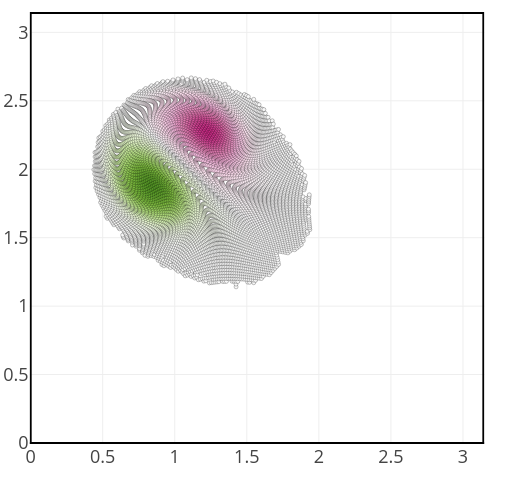
\includegraphics[width=\linewidth]{./images/app2d/assim_member_forecast.png}
		\caption{Forecast member discretization.}
	\end{subfigure}
	\hfill
	\begin{subfigure}{0.32\textwidth}
		\centering
		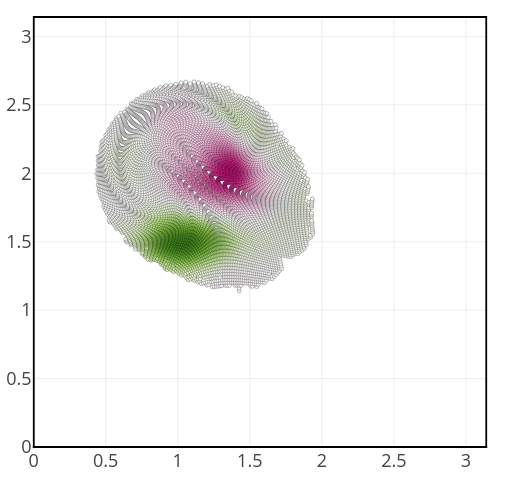
\includegraphics[width=\linewidth]{./images/app2d/assim_member_ppf.png}
		\caption{Part-EnKF analyze discretization.}
	\end{subfigure}
	\hfill
	\begin{subfigure}{0.32\textwidth}
		\centering
		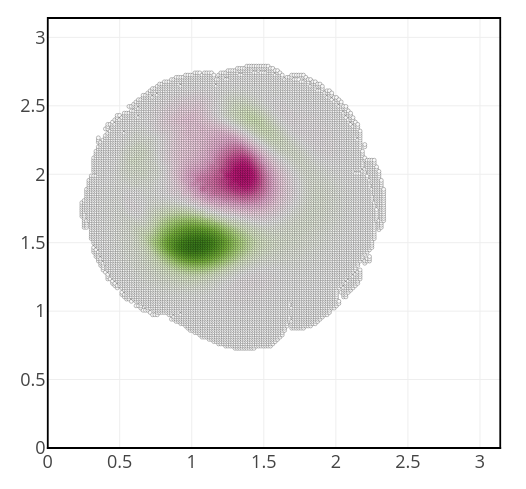
\includegraphics[width=\linewidth]{./images/app2d/assim_member_rmf.png}
		\caption{Remesh-EnKF analyze discretization.}
	\end{subfigure}
	\caption{Assimilation of one member with a forecast discretization unadapted to the analyses solution. The forecast discretization used by the Part-EnKF does not always support approximation for the analyses and introduces discretization errors.}
	\label{fig:assim_member}
\end{figure}

To evaluate the effect of the size of the support, we varied the value of $\epsilon_{\omega}$. We have seen in Figure~\ref{fig:eps_effect} that this parameter affects the number of particles and, thus, the size of the support. In Figure~\ref{fig:cuttoff}, we observe high disparities between the two filters. However, the error stabilizes rapidly by decreasing the threshold. These findings suggest an impact on the threshold and, thus, the particle support for the Part-EnKF. By contrast, Remesh-EnKF is less sensible. As a consequence, it only thresholds low values in the analyzed solutions.

\begin{figure}[h!]
	\centering

	\begin{subfigure}{0.48\textwidth}
		\centering
		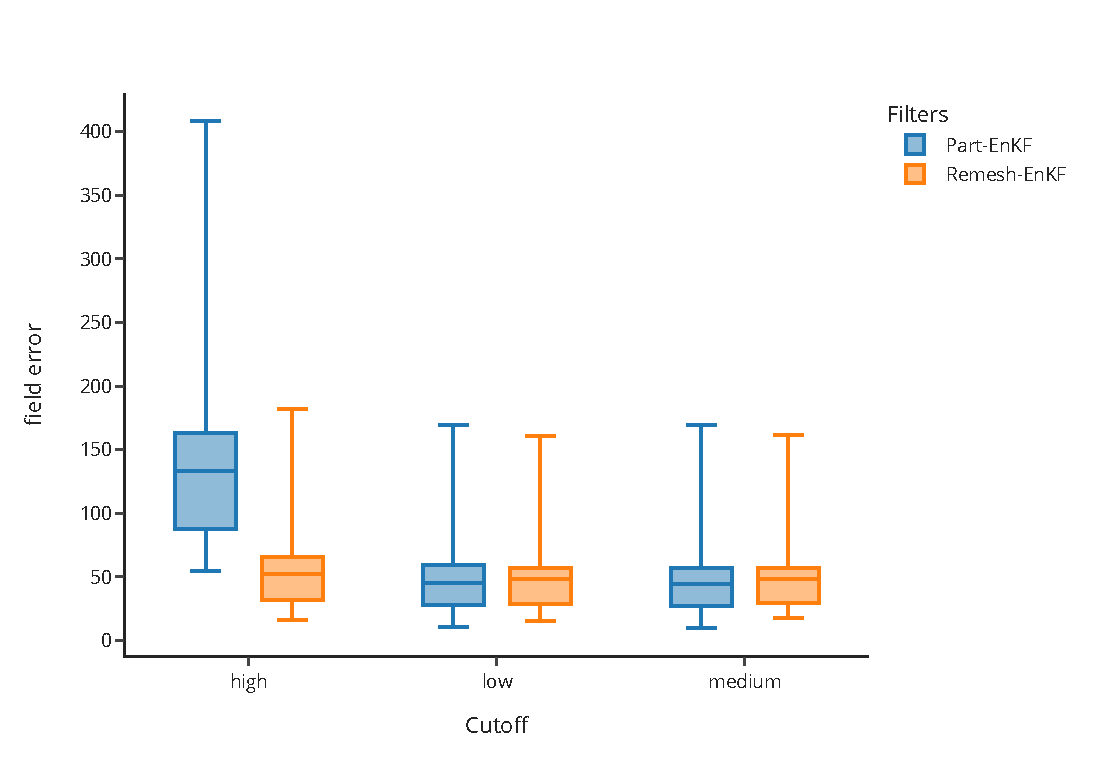
\includegraphics[width=\linewidth]{./images/app2d/final/MSE_cutoff_box.pdf}
		\caption{state error w.r.t. $\varepsilon_{\omega}$. The High, low, and medium cutoff correspond respectively to $\varepsilon_{\omega} = 0.1, 1.e^{-6}$ and $0.01$.}
		\label{fig:cuttoff}
	\end{subfigure}
	\hfill
	\begin{subfigure}{0.48\textwidth}
		\centering
		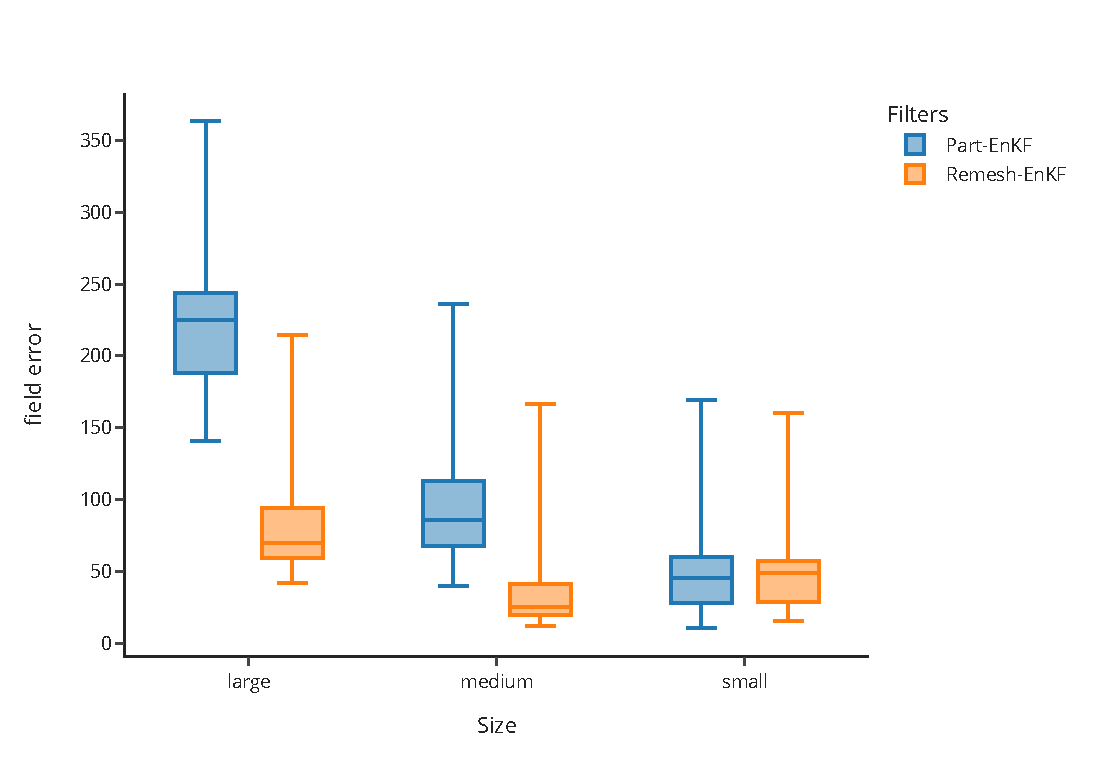
\includegraphics[width=\linewidth]{./images/app2d/final/MSE_size_box.pdf}
		\caption{state error w.r.t. $d_p$. The large, medium, and low sizes correspond to $d_p = 0.0327, 0.0245$, and $0.0123$.}
		\label{fig:np}
	\end{subfigure}

	\caption{Error box plots for simulation parameters. The effect of $\varepsilon_{\omega}$ on the error is particularly observed on high value. The Part-EnKF error is strongly linked to $d_p$ through the particle approximation error.}
	\label{fig:simu_parameters_error}
\end{figure}

In terms of particle size $d_p$, we evaluate its effect on the assimilation. In this section, we have used the regression operator defined in Section~\ref{regressionOperator} for Part-EnKF. This choice has been motivated to accelerate the update process.
in Figure \ref{fig:np}. We observe that the error for Part-EnKF and Part-Grid-EnKF increases proportionally with $d_p$ as for the approximation error. This high error confirmed, in that case, the high effect of the particle approximation for Part-EnKF. In contrast, the Remesh-EnKF error is relatively low, taking advantage of a high-order projection interpolation scheme. Using a regression operator to approximate the analyzed solution should alleviate this effect provided other particle discretization considerations (distortion, support size) as illustrated in Part~\ref{App_1D} and the choice of an adequate penalty coefficient to succeed in approximating the solution.


This discussion pointed out the high dependency of the Part-EnKF on particle discretization. The particle discretization of a member may be too far from the solution support of particles. This opens the question of the choice or modification of the particle discretization. As suggested in Part~\ref{App_1D}, an error estimation could be introduced to choose between the different filters. On the other hand, other approaches could be to select the member with the maximum likelihood estimate to approximate the solution. This proposition has to be evaluated because it could considerably reduce the variance of the ensemble. Finally, an alignment of particles might be introduced to better fit the analyzed solution.

\newpage


% !TEX root = main.tex

\section{Conclusion}
In this study, we introduce a novel framework that combines a sequential ensemble data assimilation approach with particle-based models. Specifically, we have developed two novel Ensemble Kalman Filter schemes dedicated to meshfree simulations. These formulations depend either on updating the particle quantities or on remeshing the particle discretization on a common ensemble grid.

We proposed two update strategies relying on an update matrix that does not directly depend on the state discretization. The first strategy, Remesh-EnKF, is based on the projection of every member onto a new common discretization of particles. The second strategy, Part-EnKF, evaluates the analysis field at particle locations to update the particle quantities.

The different classes have been initially tested on a one-dimensional example and compared with an Eulerian representation of the solution.The results demonstrate comparable performance across the various filters, with the exception of certain configurations of the Part-EnKF. It has been demonstrated that provided the support of the particles is consistent with the analysis solution, the filters yield similar results. However, in cases where the support deviates from the analysis field, members diverge. Increasing the support for the solution is necessary.

A two-dimensional case has also been tested, particularly to assess nonlinear advection schemes with various configurations. We observe good agreement among the different filters. However, this time, the particle approximation is predominant in the Part-EnKF.
Both strategies offer several derivations. Remesh-EnKF is mainly dependent on the redistribution kernel to obtain the new regularly spaced particle set. Part-EnKF could be extended because it is highly flexible when defining the new set of particles for each member. This tuning is essential, as we have highlighted the issue of the non-conforming support of the forward particle position with the analysis.

Several methodologies to introduce new particles or change the previous ones could be explored, particularly at the edge of the distribution.
For the sake of simplicity, we advocate generating a new set of particles with a regular spacing for any member encountering difficulties in accurately reconstructing the analysis field.
Another alternative is to update the positions of the particles in addition to the intensities instead of only changing the intensities. In this way, the error due to a misfit of alignment or approximation could be avoided. These type of adaptation could be derived from optimal transport scheme~\cite{bocquet_bridging_2023} or correction of the background ensemble alignment with the observation~\cite{ravela_data_2007,rosenthal_displacement_2017}.

\newpage
\begin{subappendices}
    % !TEX root = main.tex

\appendix
\section{Stochastic Ensemble Kalman Filter}~\label{appendix:enkf}

We define the matrix of states and the matrix of anomalies $\X_f = [\state^1, \dots, \state^N]$, $\annomX_f$ whose columns are the member states and the normalized anomalies.

\begin{equation*}
    \annomX_f = \frac{1}{\sqrt{N - 1}}(\X_f - \overline{\state}_f \bm{1}^T),
\end{equation*}where$\bm{1} \in \mathbb{R}^N$ is a vector of one.

Respectively the matrix of observation and observation anomalies are $\mathcal Y_f = [\mathcal{H}(\state^1_f), \dots, \mathcal{H}(\state^N_f)]$, $\annomY_f$ where columns are

\begin{equation*}
    \annomY_f = \frac{1}{\sqrt{N - 1}} \left(\mathcal Y_f - \overline{\obs}_f \bm{1}^T \right) \quad \text{with} \quad \overline{\obs}_f = \frac{1}{N} \sum_{j=1}^{N} \mathcal{H}(\state^j_f).
\end{equation*}

The ensemble defines the covariance between states and observations $\Cov \bm H^T$, the covariance between observations $\Cov \bm H^T$, and $\tilde{\bm{K}}$

\begin{eqnarray*}
    \Cov \bm H^T &=& \frac{1}{N - 1} \sum_{i = 1}^{N} {(\state^i_f - \overline{\state}_f)}^T {\left[ \mathcal{H}_k(\state^i_f) - \overline{\bm{y}}_f\right]}^T = \annomX_f \annomY_f^T, \\
    \bm H \Cov \bm H^T &=& \frac{1}{N -1} \sum_{i = 1}^{N}\left[ \mathcal{H}_k(\state^i_f) - \overline{\bm{y}}_f\right] {\left[ \mathcal{H}_k(\state^i_f) - \overline{\bm{y}}_f\right]}^T = \annomY_f \annomY_f^T,\\
    \tilde{\bm{K}} &=& \Cov \bm H^T{(\bm H \Cov \bm H^T + \bm R)}^{-1} = \annomX_f \annomY_f^T {(\annomY_f \annomY_f^T + \bm R)}^{-1}.
\end{eqnarray*}

This observation matrix-free implementation rely on the secant method approximation $\mathcal{H}(\state^i_f - \overline{\state}_f) \approx \predi - \overline{\obs}_f$.
The forecast is then update to a posterior ensemble ${[\state^i_a]}_{i=1}^{N}$ such as

\begin{equation} \label{enkf_formula}
    \mstate_a = \mstate_f + \tilde{\bm{K}} ( \mdata - \mpred),
\end{equation}where ${[\mdata]}^i = \obs + \bm{\varepsilon}^i$ is the perturbed observation with $\bm{\varepsilon}^i \sim \mathcal{N}(\bm{0}, \bm R) $, $\tilde{\bm{K}}$ the ensemble Kalman gain matrix and $( \mdata - \mpred)$ the innovation term.
The forecast step is then applied to the analyzed ensemble until the following observation.
Based on this formulation, we can deduce a correction formula only based on the member's predictions and observations.

We can rewrite the classical update formula using the previous anomaly matrices.

\begin{equation*}
    \mstate_a = \mstate_f + \annomX_f \annomY_f^T {({\annomY_f \annomY_f^T + \bm R})}^{-1}(\mdata - \mpred)
\end{equation*}

We reformulate the correction term by remarking that $ \bm{1}^T  \annomY_f^T = \bm{0}$. We define $\Fcorr$, the correction matrix that gives the update in terms of linear combinations of the forward states

\begin{equation*}
    \mstate_a = \mstate_f + \mstate_f \Fcorr, \quad \Fcorr = \frac{1}{\sqrt{N - 1}}\annomY_f^T {(\annomY_f \annomY_f^T + \bm R)}^{-1}(\mdata - \mpred).
\end{equation*}.

using the Sherman-Morrison-Woodbury formula we obtain

\begin{equation*}
    \Fcorr = \frac{1}{\sqrt{N - 1}} {(\bm I_N + \annomY_f^T\bm R^{-1}\annomY_f)}^{-1}\annomY_f^T \bm R^{-1} (\mdata - \mpred).
\end{equation*}
\section{Moment conservation of particle discretization}~\label{appendix:moment_conservation}

The $m$-th moment of a particle distribution is defined as the quantity $\sum_{p} z_p^{\alpha} \bm{U}_p$.

First, we see that the partition of unity is required

\begin{equation}~\label{eq:unity1}
    \sum_{I \in \Lambda} W\left(\frac{z - z_I}{\ell_I}\right) = 1 ,\quad z \in \Omega
\end{equation}~due to the final particle arrangement $\mathcal{P'}$ on a grid of size $d_p$, it leads to the following property

\begin{equation}~\label{eq:unity2}
    \sum_{p'\in\mathcal P'} W\left(\frac{z - z_{p'}}{\ell_I}\right) = \frac{V_I}{V_p'},\quad z \in \Omega.
\end{equation}.

Attention should be focused on the border. Extending the domain with "ghost" particles or nodes allows for verification of properties within $\Omega$.

This property is the necessary condition for the conservation of the first moment. Primarily for the assignment

\begin{gather}
    \begin{align*}
        \sum_{I \in \Lambda} \bm u_I V_I & = \sum_{p \in \Lambda} \bm U_p  W \left(\frac{z_I - z_p}{\ell_I} \right)                                                           & \\
                                         & = \sum_{p \in \mathcal P} \bm U_p \sum_{I \in \Lambda} W \left(\frac{z_I - z_p}{\ell_I} \right) = \sum_{p \in \mathcal P} \bm U_p. &
    \end{align*}
\end{gather}~using the property \eqref{eq:unity1}. Secondary, for the interpolation process

\begin{gather}
    \begin{align*}
        \sum_{p' \in \mathcal P'} \bm U_{p'} = \sum_{p' \in \mathcal P'} \bm u_g(z_{p'}) V_{p'} & = \sum_{p' \in \mathcal P'} V_{p'} \sum_{I \in \Lambda} \bm u_I W \left(\frac{z_{p'} - z_I}{\ell_I}\right)                                                &   \\
                                                                                                & =  \sum_{I \in \Lambda} \bm u_I  V_{p'}\sum_{p' \in \mathcal P'} W \left(\frac{z_{p'} - z_I}{\ell_I}\right)                                               &   \\
                                                                                                & =  \sum_{I \in \Lambda} \frac{V_I}{V_p'} V_{p'} \bm u_I =                            \sum_{I \in \Lambda} \bm u_I V_{I} = \sum_{p \in \mathcal P} \bm U_p & ,
    \end{align*}
\end{gather}~using equation~\eqref{eq:unity2}.

It can be shown moreover that if for $1 \leq |\alpha| \leq m - 1$, $W$ satisfies,

\begin{equation}
    \sum_{I \in \Lambda} {(\bm z-\bm z_I)}^\alpha W \left(\frac{\bm z - \bm z_I}{\ell_I} \right) = 0, \label{eq:momentProperty}
\end{equation}

The regridding procedure will be ordered at $m$. Equivalently, the previous equality lead, for $0 \leq |\alpha| \leq m - 1$, to
\begin{equation*}
    \sum_{I \in \Lambda} \bm z_I^\alpha W \left(\frac{\bm z_p - \bm z_I}{\ell_I} \right) = \bm z^\alpha,
\end{equation*}~obtained by developing ${(\bm z-\bm z_q)}^\alpha$ and using a recurrence on previous orders. This means that the interpolation is exact for polynomials of degrees less or equal to $m-1$ or that the moment of order $m-1$ is conserved.

\section{Parameters}~\label{appendix:simulation-parameters}

\subsection{One dimension problem}
\begin{table}[htbp]
    \centering
    \caption{Ensemble generation variables}
    \begin{tabular}[t]{|l|l|}
        \hline
        Variables                   & Distributions                              \\
        \hline
        Gaussian mean               & $Z_m \sim  \mathcal{N}(\meanZm, \sigmaZm)$ \\
        Gaussian standard deviation & $S_m \sim\mathcal{U}(\smLow, \smUp)$       \\
        velocity                    & $v \sim \mathcal{N}(\vmean, \vstd)$        \\
        diffusion                   & $D \sim \mathcal{U}(\Dlow, \Dup)$          \\
        \hline
    \end{tabular}
    \label{tab:ens_gen_1d}
\end{table}

\subsection{Two dimension problem}
\begin{table}[htbp]
    \centering
    \caption{Reference parameters}
    \begin{tabular}[t]{|l|l|}
        \hline
        Parameters            & Values                                                       \\
        \hline
        reference viscosity   & $v_{\text{ref}} = 0.001$                                     \\
        reference orientation & $\theta_{\text{ref}}  = \frac{7 \pi}{8} (\text{rad.})$       \\
        barycenter position   & $\bm{z}_{\text{ref}} = \left[\frac\pi2, \frac\pi2 \right]^T$ \\
        translation velocity  & $U_{\text{ref}} = 0.25$                                      \\
        \hline
    \end{tabular}
    \label{tab:ref}
\end{table}

\begin{table}[htbp]
    \centering
    \caption{Nominal assimilation and simulation parameters}
    \begin{tabular}[t]{|l|l|}
        \hline
        Parameters                      & Values                                 \\
        \hline
        time step                       & $dt = 0.005$                           \\
        final time                      & $t_f =10$                              \\
        std. observation                & $\sigma_{obs} =  5.0e^{-2}$            \\
        vorticity threshold             & $\varepsilon_{\omega} = 1.0e^{-4}$     \\
        particle characteristic length  & $dp = \frac{pi}{256} \approx 0.01227 $ \\
        smoothing length                & $h = 2.0 dp$                           \\
        number of assimilation          & $N_{\text{assim}} = 10$                \\
        ensemble size                   & $N_{\text{ens}} = 32$                  \\
        number of observation           & $N_{\text{obs}} = 12^2 = 144$          \\
        grid discretization             & $N_{\text{grid}} = 65^2 = 4225$        \\
        number of remeshing by forecast & $N_{\text{remesh}} =  2 $              \\
        \hline
    \end{tabular}
    \label{tab:simu_2d}
\end{table}

\begin{table}[htbp]
    \centering
    \caption{Ensemble generation variables}
    \begin{tabular}[t]{|l|l|}
        \hline
        Variables   & Distributions                                                                                                           \\
        \hline
        radius      & $R \sim \cN(1.0, 0.05^2)$                                                                                               \\
        orientation & $\theta \sim \cU\left(\pi, \frac\pi2 \right) (\text{rad.}) $                                                            \\
        barycenter  & $z_{\text{mean},x} \sim \cN\left(\frac\pi2,0.1^2\right), \quad z_{\text{mean},y} \sim \cN\left(\frac\pi2,0.1^2\right) $ \\
        velocity    & $U \sim \cU(0, 0.5^2) $                                                                                                 \\
        viscosity   & $v \sim \cN(0.0015, 0.0005^2)$                                                                                          \\
        \hline
    \end{tabular}
    \label{tab:ens_dipole}
\end{table}

\newpage
\end{subappendices}

% % !TEX root = main.tex

\section{Développement de méthodes permettant l'adaptation du filtre de Kalman d'ensemble avec des simulations sans maillage}

---------------
\subsection{Objectif}
Le filtre de Kalman présenté en Section~\ref*{sec:enkf} est un filtre séquentiel adéquat pour appliquer des méthodes d'assimilation pour des modèles de grande dimension et non-linéaire. Il consiste à mettre à jour un ensemble d'état en déterminant un gain de Kalman pour combiner l'état prédit et un terme d'innovation fonction de l'erreur de prédiction. Lorsque l'état est défini à l'aide d'une discrétisation eulérienne, la mise à jour du filtre peut être facilement. Il en est de même pour les états défini sur une

%
% Revoir introduction article.
%

En particulier ce gain va dépendre des statistiques de l'étatet

Toutefois, la mise à jour du filtre de Kalman d'Ensemble est dépendante de la discrétisation de l'état de ses membres pour le calcul du gain de Kalman d'ensemble. De plus, la mise à jour du filtre de Kalman d'Ensemble est basé sur une combinaison linéaire des membres au travers du gain de Kalman d'ensemble, celle-ci entraîne une explosion du nombre de particules dans la définition de la solution analysée.

L'objectif de ce chapitre est donc de présenter un certain nombre d'adaptation du filtre de Kalman d'Ensemble qui puisse être appliquées à des simulations sans maillage.

Pour cela, nous reformulons tout d'abord l'expression de la mise à jour afin qu'elle soit indépendante de la définition de l'état.
Enfin, les solutions analysées étant des combinaisons linéaires des particules de l'ensemble des membres, nous proposons de développer des méthodes pour réduire l'augmentation exponentielle des particules.

\subsection{Mise à jour défini dans l'espace des membres}

La mise à jour du filtre de Kalman se base sur l'approximation des statistiques des distributions de l'état et des observations pour approché le gain de Kalman (voir \eqref{eq:enkf_formula}).

Dans le cas d'un état qui repose sur une discrétisation particulaire, on ne peut directement évaluer ses statistiques directement sur les quantités particulaires, c'est à dire positions et intensité. En effet, chaque membre possède


Heureusement La particularité du filtre de Kalman d'ensemble est qu'il fait une approximation de faible rang du gain de Kalman. Nous avons montré en Section~\ref{sec:faible_rang} que la mise à jour s'exprimait comme une combinaison des états de l'ensemble $X$.

De cette manière la mise à jour est déterminé comme

\begin{equation*}
    \mstate_a = \mstate_f + \mstate_f \Fcorr, \quad \Fcorr = \frac{1}{\sqrt{N-1}} \annomY_f^T {(\annomY_f \annomY_f^T + \bm R)}^{-1}(\mdata - \mpred).
\end{equation*}.

Où la matrice de correction $\Fcorr \in \mathbb{R}^{N\times N}$ est indépendante de la discrétisation.

De plus, en utilisant la formule de Sherman-Morrison-Woodbury (SMW)~\cite{SMW}, la matrice peut être calculé à l'aide uniquement de l'inversion de la matrice $\bm R$ et d'une matrice de taille $N$

\begin{equation*}
    \Fcorr = \frac{1}{\sqrt{N - 1}} {(\bm I_N + \annomY_f^T\bm R^{-1}\annomY_f)}^{-1}\annomY_f^T \bm R^{-1} (\mdata - \mpred),
\end{equation*}ce qui devient avantageux dans le cas où $\bm R$ est une matrice diagonale et $N < N_{\text{obs}}$.

Cette indépendance est possible par la linéarisation de l'opérateur d'observation et l'approche par rang faible. D'autres versions du filtre EnKF offre les mêmes propriétés. C'est le cas du \textit{ensemble transform Kalman filter} (ETKF, \cite{Hunt2007}). En effet, ce filtres travaillent directement dans l'espace de perturbation.

Travailler dans l'espace de perturbation des observations $\bm Y^T$ permet d'éviter d'exprimer les statistiques de l'état.

L'étape d'analyse est donc une combinaison qui ne dépend que des observations $\bm y$ (perturbé pour le filtre stochastique), les prédictions de l'ensemble $\left[\mathcal{H}(x^i_f)\right]_{i=1}^{N}$, et la matrice de covariance d'erreur $R^{1}$. De cette manière, pour chaque membre $i$, le champ analysé $\fstate_i^a$ peut être déterminé en tout point de l'espace $\bm x \in \omega$ grâce aux champs prédits $\fstate_j^f$ tel que

\begin{equation}
    \fstate_i^a(\bx) =\fstate_i^f(\bx) + \sum_{j=1}^{N} F_{ji} \fstate_j ^f(\bx), \quad i = 1, \dots, N.
\end{equation}

\subsection{Mise à jour comme solution particulaire}

Les solutions analysées peuvent être décomposées à partir de la discrétisation particulaire des champs $\fstate_i^f$.

Dans un premier temps, nous supposons que les positions de particules sont les mêmes pour tous les membres. On note $(\bx_1,...\bx_{N_p}) \in \mathbb{R}^d$ les positions des centres de particule, deux à deux distincts de telle sorte que, pour tout $\bx \in \mathbb{R}^d$

\begin{eqnarray*}~\label{eq:enkf_formula_same_part}
    \fstate_i^a(\bx) &=& \fstate_i^f(\bx) + \sum_{j=1}^{N} F_{ji} \fstate_j ^f(\bx) \\
    &=& \sum_{p=1}^{N_p} \Gamma^f_{p,i} \phi_{\varepsilon}(\bx - \bx_p) + \sum_{j=1}^{N} F_{ji} \sum_{p=1}^{N_p} \Gamma_j ^f(\bx) \phi_{\varepsilon}(\bx - \bx_p) \\
    &=& \sum_{p=1}^{N_p} \left[\Gamma^f_{p,i} + \sum_{j=1}^{N} F_{ji} \Gamma^f_{p,j} \right] \phi_{\varepsilon}(\bx - \bx_p).
\end{eqnarray*}

En utilisant la linéarité de la décomposition par rapport aux intensités $\Gamma^f_{p}$, l'analyse pour chaque membre peut directement s'exprimer pour chaque membre en appliquant la mise à jour directement sur les intensités. En notant $\bm \Gamma$ la matrice dont la i-ème colonne est $(\Gamma_{1, i},...\Gamma_{N_p, i})$, la mise à jour est directement exprimé comme

\begin{equation*}
    \bm \Gamma^a = \bm \Gamma + \bm \Gamma \Fcorr.
\end{equation*}

Cependant, dans le cas général les positions de particules diffèrent d'un membre à l'autre. Dans ce cas, en utilisant la décomposition particulaire des champs prédit $\mP_i^f$, la solution analysée va s'exprime comme

\begin{eqnarray*}
    \fstate_i^a(\bx) &=& \sum_{p \in \mP_i^f}\Gamma^f_p \phi_{\varepsilon}(\bx - \bx_p) + \sum_{j=1}^{N} F_{ji}  \sum_{p' \in \mP_j^f}\Gamma^f_{p'} \phi_{\varepsilon}(\bx - \bx_{p'}) \\
    &=& \sum_{p \in \mP_i^f}\left[(1 + F_{ii})\Gamma^f_p \phi_{\varepsilon}(\bx - \bx_{p})\right]   + \sum_{j\neq i} F_{ji} \Gamma^f_{p'} \phi_{\varepsilon}(\bx - \bx_{p'})\\
    &=& \sum_{j=1}^{N} \sum_{p \in \mP_j^f} \Gamma^a_p \phi_{\varepsilon}(\bx - \bx_p).
\end{eqnarray*}
$\fstate_i^a$ est bien une solution particulaire.


Sans perte de généralité, en supposant que chaque particules ont des positions $x_p$ distincts, alors l'espace d'approximation est de dimension $\sum_{i=1}^{N} \text{Card}(\mathcal{P}^f_i)$.

Ainsi, à chaque étape d'assimilation de données, le nombre de particule pour approcher la solution analysée augmente exponentiellement avec l'union des particules de tous les membres comme en Figure~\ref{fig:support_particles}.

\begin{figure}~\label{fig:support_particles}
    \centering
    \begin{subfigure}{0.5\textwidth}
        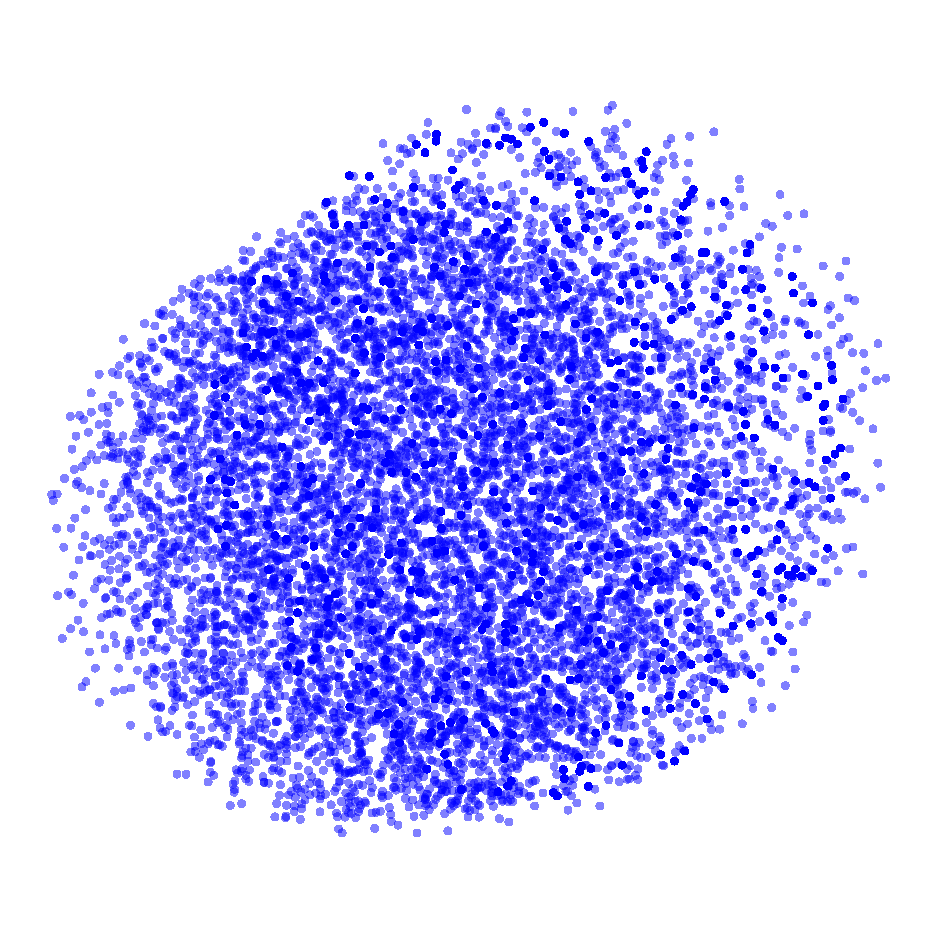
\includegraphics[width=\textwidth]{./images/all_particles.pdf}
    \end{subfigure}
    \begin{subfigure}{0.5\textwidth}
        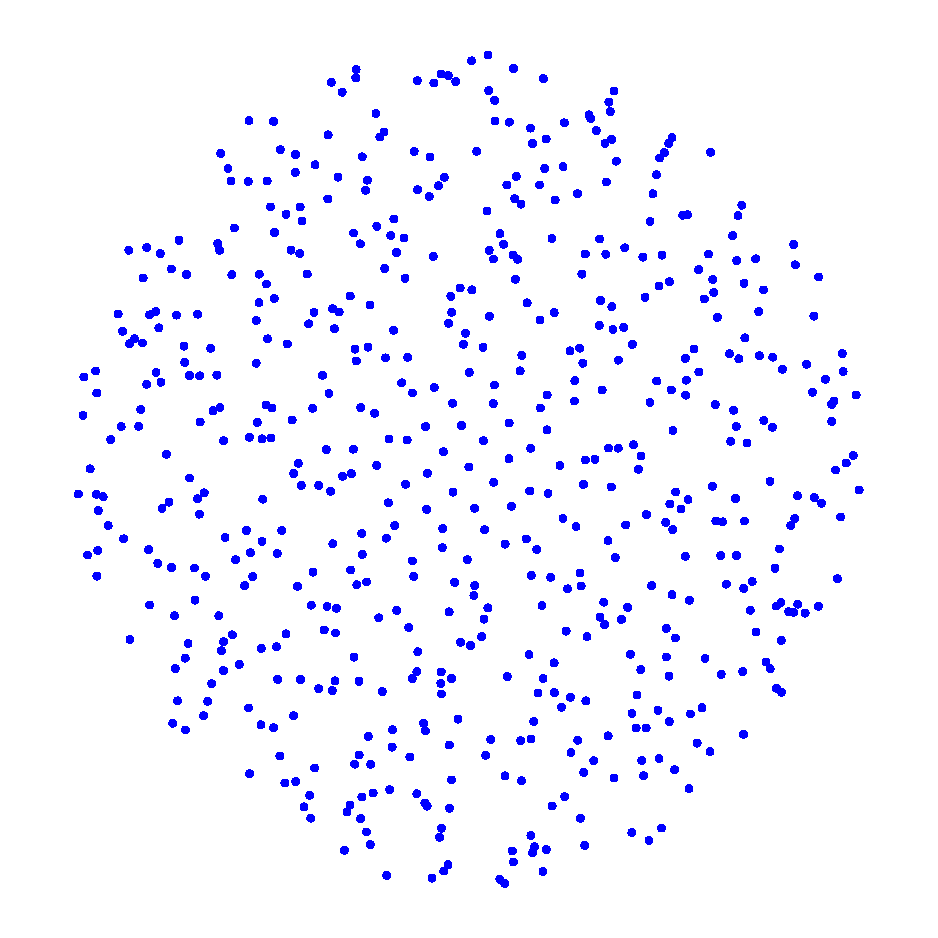
\includegraphics[width=0.5\textwidth]{./images/memb_particles.pdf}
    \end{subfigure}
    \caption{Support de particule d'un membre avant et après correction.}
\end{figure}

Cette mise à jour ne peut donc pas être mise en pratique. Il est nécessaire de proposer des méthodes pour réduire le nombre de particules pour représenter la solution analyser. Afin de résoudre ce problème, nous proposons deux approches distinctes:

\begin{itemize}
    \item \textbf{Remesh-EnKF}: \\
    \item \textbf{Part-EnKF}: \\
\end{itemize}

\subsection{Remesh-EnKF : Générer une même configuration particulaire}

Cette méthode consiste à revenir à un ensemble de particules définis sur un support commun. En remaillant régulièrement, nous pouvons contrôler et limiter le nombre de particules, assurant ainsi une représentation plus homogène et gérable de la solution. Le remaillage permet de maintenir une distribution équilibrée des particules, tout en préservant les caractéristiques essentielles de la solution originale.

\subsubsection*{Méthode de remaillage pour obtenir un support de particule commun}~\label{sec:remesh}

La méthode de remaillage est une technique essentielle dans notre approche pour maintenir un support de particule uniforme parmi tous les membres de la solution. À l'origine développée pour atténuer les distorsions dans la distribution des particules, cette méthode se fonde sur un schéma de redistribution sur une grille régulière de particules, utilisant des opérateurs de projection et d'interpolation. Ce processus permet de passer d'une représentation lagrangienne à une représentation eulérienne, puis ensuite revenir à une représentation lagrangienne.

L'essence de cette méthode réside dans l'utilisation d'opérateurs similaires à ceux employés par les méthodes Particles in Cell (PIC) comme la méthode \textit{Vortex-In-Cell} (VIC) ou la \textit{Material Point Method} (MPM).

Le remaillage est défini en deux étapes.

Consiste en un schéma de redistribution sur une grille régulière de particules à l'aide d'opérateur de projection et d'interpolation. Elle consiste à passer d'une représentation lagragienne à eulérienne, puis de revenir sur une grille de particules lagrangienne. En fait même type d'opérateur qu'utilisé par les méthodes particules in cell (PIC).

Dans notre méthodologie, nous proposons une approche en deux étapes. Tout d'abord, nous effectuons une étape d'assignation (\ref{assigment}) pour transférer la discrétisation des particules à une discrétisation sur une grille. Ensuite, une étape d'interpolation (\ref{interpolation}) est réalisée pour obtenir un nouvel ensemble de particules régulièrement espacées.

Notre analyse se rapporte au scénario unidimensionnel, où $\Omega \in \mathbb{R}$. L'extension au cas $n$-dimensionnel peut être réalisée par la tensorisation de l'approche unidimensionnelle.

\begin{enumerate}[label=(\alph*)]
    \item \textit{Affectation sur une grille eulérienne} \label{assigment}

          Nous désignons par $z_{I}$ et $z_{p}$ respectivement les emplacements sur la grille et les anciens emplacements des particules. Les nouvelles particules sont définies sur une grille de $n_g$ éléments avec un espacement régulier $\ell_I = 2 d_p$, où $d_p$ est la taille caractéristique des particules. Nous définissons les intensités des particules comme $\bm U_p$ et les valeurs du champ nodal comme $\bm u_I$. En utilisant une fonction de forme $W$, l'étape d'affectation des particules à chaque nœud $I \in \Lambda$ peut être écrite comme

          \[
              \bm{u}_I = \frac{1}{V_I} \sum_{p \in \mathcal{P}} \bm U_p  W \left(\frac{z_I - z_p}{\ell_I} \right).
          \]

          Où $W$ détermine une redistribution de l'intensité sur la grille, la nouvelle discrétisation peut ensuite être utilisée pour approximer le champ $\bm{u}_p$, défini par la discrétisation des particules par interpolation

          \[
              \bm{u}_p(z) \approx \bm{u}_g(z) = \sum_{I \in \Lambda} \bm u_I W \left(\frac{z - z_I}{\ell_I} \right) \quad \forall z \in \Omega.
          \]

    \item \textit{Interpolation sur une nouvelle discrétisation régulière des particules} \label{interpolation}

          Un nouvel ensemble de particules est défini au quart de chaque cellule de sorte que la nouvelle position est définie à $z_{p'} = d_p/2 + i~dp, \quad i = 0,\dots, 2n_g $. La valeur du champ est alors interpolée à cette nouvelle position et multipliée par le volume de la particule $\bm{U}_{p'} = \bm  u_g(z_{p'}) V_{p'}$ afin de donner une nouvelle approximation particulaire de ce champ

          \[
              \bm{u}_g(z)  \approx \bm{u}_{p'}(z) = \sum_{p'\in\mathcal{P'}} \bm{u}_g(z_{p'}) V_p,
          \]

\end{enumerate}

La combinaison de ces deux étapes peut être initialement utilisée pour générer une nouvelle distribution de particules non déformées. La fonction de forme $W$ détermine le type et la qualité du transfert. Le critère de la qualité de la méthode réside dans la conservation des premiers moments des distributions de particules, comme détaillé en Annexe~\ref{appendix:momentConservation}.

Pour $W$, on peut utiliser une fonction d'interpolation afine, qui garantit la conservation du moment 0. Pour une conservation des moments supérieurs, la fonction B-spline fournit une fonction de lissage d'ordre plus élevé.

Monaghan~\cite{monaghan_extrapolating_1985} propose une approche systématique pour améliorer la précision et maintenir la régularité par extrapolation. Le concept implique la construction d'une nouvelle fonction de forme basée sur une coupure et sa dérivée radiale. Pour $m = 4$, la B-spline cubique est améliorée par le noyau d'interpolation suivant

\begin{eqnarray*}~\label{cubic_radial_kernel}
    M_4'(z) &=& \left{ \begin{aligned}
         & 1 - \frac{5}{2}z^2 + \frac{3}{2} |z|^3 & 0 \leq & |z| \leq 1 & \
         & \frac{1}{2}{(2 - |z|)}^2(1 - |z|)      & 1 \leq & |z| \leq 2 & \
         & 0                                      & 2 \leq & |z|.
    \end{aligned}
    \right.
\end{eqnarray*}

que nous utiliserons dans les applications.

Enfin, dans l'espace multidimensionnel, le noyau de redistribution $W$ peut être obtenu comme le produit du noyau unidimensionnel appliqué à chaque coordonnée, comme suit

\begin{eqnarray*}
    \bm U_p &=& \sum_{I \in \Lambda} \bm U_I W \left(\bm z_p - \bm z_I, \ell_I \right) \
    &=& \sum_{I \in \Lambda} \bm U_I \prod_{i = 1}^d W_{1\text{D}} \left(\frac{\bm z_{I, i} - \bm z_{p, i}}{\ell_I} \right)
\end{eqnarray*}

Le schéma est illustré dans la Figure~\ref{fig:remaillage}

\begin{figure}~\label{fig:remaillage}
\end{figure}

\subsubsection*{Algorithme}

Le filtre Remesh-EnKF utilise les opérateurs précédemment définis pour appliquer la mise à jour de EnKF. L'assimilation est effectuée avec les étapes suivantes :

\begin{itemize}
\begin{itemize}
    \item \textit{propagation} : Les membres sont propagé, étant donné un nouvel ensemble de particules $\mathcal{P}^f_i = {(\bm z^f_{ip}, \bm U^f_{ip})}{ip = 1}^{N{ip}}$,
    \item \textit{projection}: Le champ associé est projeté sur une grille régulière de $n_g$ éléments de longueur caractéristique $\ell_{iI}= 2dp$. En utilisant l'opérateur de projection~\ref{assigment}, nous obtenons pour chaque noeud $iI \in \Lambda_{i}$
          \begin{equation*}
              \bm{u}^f_{iI} = \frac1{V_{iI}} \sum_{ip \in \mathcal P^f_i} \bm U^f_{ip} \bm W \left(\frac{\bm z_{iI} - \bm z^f_{ip}}{\ell_{iI}} \right)
          \end{equation*}
    \item \textit{analyse}: Sur la base de cette nouvelle discrétisation, la mise à jour EnKF est appliquée aux valeurs d'état nodal $\bm{u}^f_{iI}$, tel que l'état d'analyse $\bm{u}{iI}^a$ est
          \begin{equation*}
              \bm{u}^a{iI} = \bm{u}^f_{iI} + \sum_{j=1}^{N_{\text{ens}}} F_{ji} \bm{u}^f_{jI},
          \end{equation*}
    \item \textit{interpolation}: Une nouvelle discrétisation régulière des particules est initialisée. Deux particules par direction sont placées à l'intérieur de chaque cellule de la grille. Les nouvelles intensités de particules sont évaluées grâce à l'opérateur d'interpolation~\ref{interpolation}, tel que $ip' \in \mathcal P_i^a$
          \begin{equation*}
              \bm U_{ip'}^a = \sum_{iI \in \Lambda} \bm u^a_{iI} \left(\frac{\bm z_{iI} - \bm z_{ip'}}{\ell_{iI}} \right).
          \end{equation*}
\end{itemize}

Les différentes étapes sont résumés dans l'algorithm~\ref{algo:remesh_enkf}

\begin{algorithm}

    \caption{Remesh Filter analysis update}~\label{algo:remesh_enkf}

    \KwData{$\bm G \in \mathbb R^{n_g \times d}, \bm z^a \in \mathbb R^{2 n_g \times d}$ \tcp*[r]{grille}}
    \KwData{$\bm R \in\mathbb{R}^{m}$  \tcp*[r]{covariance des observations}}
    \KwIn{$\mathcal{P}^f_i= \{(\bm z^f_{ip}, \bm U^f_{ip})\}_{ip = 1}^{N_{ip}}, \quad i = 1, \dots, N_{\text{ens}}$ \tcp*[r]{forward discretizations}}
    \KwIn{ $\bm Y_f \in \mathbb{R}^{m \times N_{\text{ens}}}$ \tcp*[r]{the associate observation anomalies}}
    \KwIn{$\bm D \in \mathbb{R}^{m \times N_{\text{ens}}}$  \tcp*[r]{the perturbed observations}}

    $ \Fcorr = \frac{1}{N-1}\annomY_f^T {(\annomY_f \annomY_f^T + \bm R)}^{-1}(\mdata - \mpred)$ \tcp*[r]{correction matrix}
    \SetKwFunction{proj}{Projection}
    \SetKwFunction{assign}{Assign}
    \ForEach{$i = 1, \dots, \nens $}{
        $\bm u[:,i] =$ \proj{$\mathcal{P}^f_i, \bm G$}
    }
    $\bm u = \bm u + \bm u \Fcorr$ \tcp*[r]{analysis update}
    \ForEach{$i = 1, \dots, \nens $}{
    $\bm z^a_{ip}, \bm U^a_{ip} = $ \assign{$\bm u[:,i]$}
    }
    \Return{$\mathcal{P}^a_i=\{\bm z^a_{ip}, U^a_{ip}\}_{ip = 1}^{N_{a}}, \quad i = 1, \dots, N_{\text{ens}}$ \tcp*[r]{analyse discretizations} }
\end{algorithm}


On remarque que tous les opérateurs que nous avons définis sont linéaire. Ainsi, effectuer la mise à jour sur la grille comme dans l'algorithme, ou bien sur les nouvelles particules comme dans l'équation~\eqref{eq:enkf_formula_same_part} est équivalent car la mise à jour lors de l'analyse, l'opération d'interpolation ainsi que la projection sont linéaires par rapport aux intensités.
Cependant, l'ordre de l'algorithme actuel permet de réaliser le minimum d'opération sur les espaces de plus faible dimension, c'est à dire sur la grille de projection.

\subsection{Part-EnKF : Mise à des intensités}

L'adaptation précédente du filtre EnKF permet de contrôler le nombre de particule lors de l'analyse en regénérant une nouvelle distribution de particules. D'une certaine manière, elle consiste à projeter la solution sur une discrétisation eulérienne pour ensuite appliquée l'analyse de manière classique.
Dans cette partie, nous souhaitons pouvoir appliquer la mise à jour à partir uniquement des discrétisations particulaires et en conservant la distribution de particule obtenue au moment de l'assimilation. L'objectif est aussi de pouvoir traiter le cas de modèle où la génération d'une nouvelle discrétisation de particules par redistribution est impossible et de proposer une implémentation entièrement sans maillage.
Ainis, nous garderons les positions à la fin de la propagation inchangée et modifions uniquement les intensités de particules.

Ainsi, les champ analysés $u_i^a$ définis comme combinaison de l'ensemble des particules de tous les membres, doivent être approché sur le support de chaque membre

\begin{eqnarray*}
    \fstate_i^a(\bx) =  \sum_{i=1}^{N} \sum_{p \in \mP_j^f} \Gamma^a_p \phi_{\varepsilon}(\bx - \bx_p)\approx \sum _{p \in \mP_i^f}
\end{eqnarray*}

Ainsi, l'analyse consiste déterminer, pour chaque membre $i$, comment mettre à jour les coefficient $Gamma^f_{ip}$ pour approcher au mieux la fonction $\fstate_i^a$.

\subsubsection{Approximation d'un champs continu par une discrétisation particulaire}

Différentes méthodes ont pu être introduites pour approcher une fonction $\bm u$ par une discrétisation particulaire. Ceci est particulièrement utile lors de l'initialisation ou bien pour réduire les effets de distorsion de la distribution particulaire.

\paragraph{Approximation particulaire}

Cette première méthode consiste à utiliser les particules comme point de quadrature. Comme dans les hypothèses initiales des méthodes particulaires~\eqref{eq:part_approx}, il convient alors d'évaluer le champ à la position des particules $x_p$ afin d'obtenir une approximation de l'intensité comme intégration locale du champ

\begin{equation*}
    \bm \Gamma^a_p = \int_{\Omega_p} \bm u^a(\bx) d\bx = \bm u(\bx_p) V_p, \quad $p \in \mathcal P^f_i$
\end{equation*}.

Si cette approximation est très simple à évaluer mais ne garantie pas d'obtenir une bonne approximation du champ si la qualité de la quadrature est de mauvaise qualité. Ceci est particulièrement le cas si la distribution particulaire n'est pas uniforme ou ne recouvre par entièrement le domaine $\Omega$.

\paragraph{Régression RBF}

Afin d'avoir une meilleure évaluation du champ en chaque position de particules $\bx_p$, Beale~\cite{beale_accuracy_1988} introduit une méthode itérative afin de déterminer les intensités $\Gamma_p$ tel que

\begin{equation*}
    \sum_{q \in P^f} \Gamma_p \phi_\varepsilon(\bx_p - \bx_q) = \fstate^a(\bx_p), \quad p \in \mathcal{P}^f.
\end{equation*}

En réalité, cette méthode revient à résoudre un problème de régression. C'est cette dernière approche qui a été développé par Barba et al.~\cite{barbara} pour modifier les . Ce sont ces méthodes qui sont également ce types de méthodes qui sont courrament utilisées pour la résolution d'EDP avec des fonctions à base radiales~\cite{Fornberg_Flyer_2015}.

On cherche à déterminer les intensités de particule définies sous la forme d'un vecteur $\bm{U} = [\bm U_1, \dots, \bm U_p]^T$. On suppose la valeur du champ à approcher $\fstate^a$ connu en position des particules et dont les évaluations sont consignés dans un vecteur $\bm{u} = [\bm u_1(z_1), \dots, \bm u_p(\bm z_p)]^T$. L'approximation particulaire peut être évalué en chaque position $\bx_p$ et doit permettre d'approcher en ces points le vecteur $\bm{u}$ comme

\begin{equation*}
    \bm{u} \simeq \tilde{\bm u} = \bm \Phi \bm{U},
\end{equation*}où $\bm \Phi_{ij} = \phi_\varepsilon(z_i - z_j)$.

Minimiser l'erreur quadratique entre la prédiction $\tilde{\bm u}$ et $\bm{u}$ revient à résoudre le problème suivant

\begin{equation*}
    \bm{U}^*= \argmin_{\bm{U}} \norm{\bm{u} - \Phi \bm{U}}^2_2.
\end{equation*}

L'opérateur étant linéaire, la solution de ce problème n'est autre que $\bm U^*  = (\bm \Phi^T \bm \Phi)^{-1} \bm \Phi \bm{u}$. Cependant, ce problème peut être mal conditionné. En particulier dans le cas où les particules sont mal distribuées (cas dégénéré lorsque deux particules se superposent). Pour éviter ces cas, un terme de pénalisation sur l'amplitude du vecteur d'intensité $\bm{U}$ est introduit. En introduisant un régularisation à la Thikhonov de la forme $\lambda \norm{\bm U}_2^2$, on obtient un problème dit de régression \textit{Ridge}, où le coefficient $\lambda$ est le coefficient de pénalisation. Le problème devient alors

\begin{equation*}
    \bm{U}_{\text{ridge}}^* = \argmin_{\bm{U}} \norm{\bm{u} - \bm \Phi \bm{U}}_2^2 + \lambda \norm{\bm{U}}^2_2,
\end{equation*}donnant la solution suivante $\bm{U}^*_{\text{ridge}} = (\bm \Phi^T \bm \Phi + \lambda \bm I)^{-1} \bm \Phi \bm{u}$.

Finalement, cette adaptation du filtre EnKF permet d'approcher les solutions analysées pour chaque membres, en modifiant uniquement les intensités de particule des membres en question. De cette manière, nous évitons l'accroissemen excessif du nombre de particules. De plus, elle permet d'être entièrement définie sans étape de remaillage.

\subsubsection{Algorithme}

Tout comme le filtre Remesh-EnKf, la première étape consiste à calculer le terme de correction $\Fcorr$ afin de pouvoir évaluer les champs analysés $\fstate_i^a$ pour chaque membre $i$. Puis le filtre Part-EnKF formule l'analyse comme une mise à jour des intensités. La représentation lagrangienne de la solution à la fin de l'étape de propagation est conservée autant que possible. Il est alors nécessaire d'évaluer les $\fstate_i^a$ au centre des particules $\bx_{ip}$, pour pouvoir approcher les intensités $\bm U_{ip}$ avec les méthodes d'approximation ci-dessus.

Les différentes étapes sont résumés dans l'algorithm~\ref{algo:part_enkf}
% \setcounter{algocf}{2}
\begin{algorithm}
    \caption{Part-EnKF Filter analysis update}~\label{algo:part_enkf}
    \KwData{$\bm R \in\mathbb{R}^{m}$  \tcp*[r]{observation covariance}}
    \KwIn{$\mathcal{P}^f_i= \{(\bm z^f_{ip}, \bm U^f_{ip})\}_{ip = 1}^{N_{ip}}, \quad i = 1, \dots, N_{\text{ens}}$ \tcp*[r]{forward discretizations}}
    \KwIn{ $\bm Y_f \in \mathbb{R}^{m \times N_{\text{ens}}}$ \tcp*[r]{the associate observation anomalies}}
    \KwIn{$\bm D \in \mathbb{R}^{m \times N_{\text{ens}}}$  \tcp*[r]{the perturbed observations}}

    $ \Fcorr = \frac{1}{N-1}\annomY_f^T {(\annomY_f \annomY_f^T + \bm R)}^{-1}(\mdata - \mpred)$ \tcp*[r]{correction matrix}
    \SetKwFunction{approxim}{Approx}
    \SetKwFunction{evaluate}{AnalysisFieldValues}
    \ForEach{$i = 1, \dots, \nens $}{
    $\bm u^a_{ip} =$ \evaluate{$\mathcal{P}^f_i, \Fcorr$} \tcp*[r]{evaluate the analysis field}
    $\bm U^a_{ip} =$ \approxim{$\bm u^a_{ip}$} \tcp*[r]{approximate the analysis field}
    }
    \Return{$\mathcal{P}^a_i=\{\bm z^f_{ip}, \bm U^a_{ip}\}_{ip = 1}^{N_{ip}}, \quad i = 1, \dots, N_{\text{ens}}$ \tcp*[r]{analyse discretizations}}
\end{algorithm}

\subsection{Complexité}

Avant d'évaluer la précision des deux filtres, nous comparons d'abord leur complexité computationnelle.

Indépendemment du cas, il est nécessaire de déterminer la matrice de correction $\Fcorr$. Dans le cas où $\bm R$ est une matrice diagonal, le calcul de $\Fcorr$ nécessite de pouvoir inverser une matrice symétrique définie positive de taille $N\timesN$ soit de l'ordre de $\mathcal O (N^3)$.

Dans le filtre Remesh-EnKF, la complexité est dominée par l'étape de remaillage pour l'ensemble de taille $N$é~\ref{sec:remesh}. En effet, dès lors que la représentation de l'état est projeté sur une même grille, elle se réduit à une multiplication matricielle.
L'étape de redistribution nécessite une boucle sur les $N_p$ particles du membre. Ainsi, si la taille du noyau de redistribution couvre $N_k$ noeuds, la redistribution d'une particule nécessite $N_k^d$ évaluations du noyau où $d$ est la dimension de l'espace. Finalement, l'étape d'interpolation demande dévaluer le champ en des points de l'espace fixe. Les poids peuvent être calculé Ainsi la complexité est du filtre Remesh-EnKF est en $\mathcal{O} (NN_pN_k^d)$. Le filtre est fortement parallélisable que cela soit sur les membres de l'ensemble ou bien sur les particules pour la projection et l'interpolation.

D'autre part, le filtre Part-EnKF est dominé par l'étape d'évaluation des champs analysées ainsi que l'étape d'approximation ou de regression. Tout d'abord, les champs sont évalués sur toutes les positions des particules de chaque membre, ce qui revient à évaluer le noyau $\phi_\varepsilon(\bx_p -\bx_q)$ pour tout couple de particules $(p, q)$. Cette fonction de forme étant nulle en dehors du domaine d'influence, ainsi $\phi_\varepsilon(\bx_p -\bx_q)$ ne doit être évalué que pour des particules $q$ dans le voisinage de $p$. Outre l'utilisation d'algorithme d'arbres de tris comme le \textit{KD-Tree}~\cite{bentley_1975_kdtree}, un algorithme de recherche sur grille peut être utilisé. Dans ce dernier cas, chaque particule est associée à une cellule d'une grille de taille $N_g$.

Une boucle est effectuée sur les cellules de la grille $N_g^d$, et la distance des particules d'une cellule est calculée avec les cellules environnantes. Nous approximons le nombre moyen de particules dans chaque cellule comme $N_{PIC} = \frac{NN_p}{N_g^d}$. Ainsi, la complexité est estimée à $\mathcal{O}(NN_p)$.

Puis les intensités $\bm U_p$ des particules doivent être calculées. L'approximation de l'intensité comme $U_p = \fstate V_p$, n'ajoute pas de complexité supplémentaire. Cependant, une méthode de régression, nécessite de résoudre $N$ systèmes linéaires indépendant de taille $N_p$. Si la matrice $\Phi$ est connue grâce aux évaluations précédentes, la résolution nécessite l'inversion d'une matrice $N_p$. Cette étape utilise un algorithme de gradient conjugué, le meilleur solveur pour un système creux. Dans ce cas, la complexité est d'environ $\mathcal{O}((N_0 + N_p) k)$ où $k$ est le nombre d'itérations et $N_0$ est la valeur non nulle de la matrice à inverser, qui est d'environ $\mathcal{O}(N_p)$. En réunissant le tout, la complexité est d'environ $\mathcal{O}(kNN_p)$. Finalement la complexité totale est d'environ $\mathcal{O}((k+1)NN_p)$.

\subsection{Bilan}

Nous avons développé deux adaptations du filtre EnKF adaptées au cas des simulations particulaires. Celle-ci tienne compte d'une augmentation exponentielle de particules.
Ces deux adaptations Remesh-EnKF et Part-EnKF correspondent à deux paradigmes. Dans le premier cas, le choix a été fait de regénérer complètement la discrétisation à l'aide de méthode de transfert particule à grille et de remaillage. Dans le second cas, le choix a été fait de conserver la position des particules de chaque membre et d'approcher la solution analysée.
Si ces filtres offre des adaptations du filtre de Kalman d'Ensemble, ils semblent souffrir de plusieurs limitations inhérantes à leur schéma. Dans la prochaine section, leur capacité d'assimilation va être vérifié sur plusieurs applications données.


% \chapter{Evaluation de la capacité des méthodes développées à assimiler les données sur plusieurs applications}
\newcommand{\xx}{x_0 = 0.02}
\newcommand{\sigx}{\sigma_0^2 = 0.5}
\newcommand{\npart}{$N_{part} = 100$}
\newcommand{\ngrid}{$N_{grid} = 100$}
\newcommand{\sigmaY}{0.05}

\section{Objectif}

Deux adaptations du filtre EnKF ont été proposées pour permettre l'assimilation de données pour des méthodes sans maillages. En effet, la correction à la Kalman entrainait des solutions dont le nombre de particules augmentait de manière exponentiel. Ainsi les méthodes ont consisté soit à générer une nouvelle distribution de particule (filtre Remesh-EnKF), soit approcher la solution analysée en modifiant les intensités des configurations particulaires de chaque membre (filtre Part-EnKF). Afin de valider ces deux approches, deux études ont été réalisées. La première présente une méthode unidimensionnelle d'un problème d'advection-diffusion. L'objectif est de mieux visialiser les différentes approches et de les comparer à une solution définies par une discrétisation eulérienne. Dans un second temps, les deux filtres sont appliqués à à un problème d'écoulement incompressible bidimensionnel non linéaire, résolu via la méthode Vortex-In-Cell (VIC) pour évaluer qualitativement le comportement des différents filtres.

\section{Problème 1D d'advection diffusion}~\label{sec:App_1D}

\subsection{Définition du problème}
Nous définissons un problème de convection-diffusion unidimensionnel $2\pi$-périodique suivant l'équation

\begin{equation*}
    \frac{\partial u}{\partial t}(x,t) + v \frac{\partial u}{\partial x}(x,t) = \visc \frac{\partial^2 u}{\partial x^2}(x,t),
\end{equation*}

avec $x$ la coordonnée spatiale, $v$ une vitesse constante et $\visc$ un coefficient de diffusion constant.
Pour l'application suivante, la solution de référence utilise les paramètres $v = \refv$ et $\visc = \refvisc$.
Nous définissons le noyau de chaleur périodique $2\pi$ en une dimension comme suit

\begin{equation*}
    \phi(u, s) = \sum_{k=-\infty}^{\infty} \frac{1}{\sqrt{4 \pi s}} \exp{\left(-\frac{{(u - 2\pi k)}^2}{4s} \right)}.
\end{equation*}

Considérant une condition initiale caractérisée par une forme gaussienne exprimée comme $u^{gt}(x, 0) = \phi(x-x_0, Dt_0)$, où $\xx$, $t_0 = \frac{\sigma_0^2}{2D}$, et $\sigx$, nous dérivons la solution analytique complète en utilisant la solution de l'équation de Green :

\begin{equation*}
    u^{gt}(x, t) = \phi(x- v t - x_0, \visc (t+t_0)).
\end{equation*}

La solution analytique est alors une fonction gaussienne, caractérisée par une moyenne qui se déplace à la vitesse d'advection et une déviation standard proportionnelle à $t$ et $D$. Cette solution est illustrée dans la Figure~\ref{fig:1d_analytical} à différents pas de temps

\begin{figure}[ht]
    \centering
    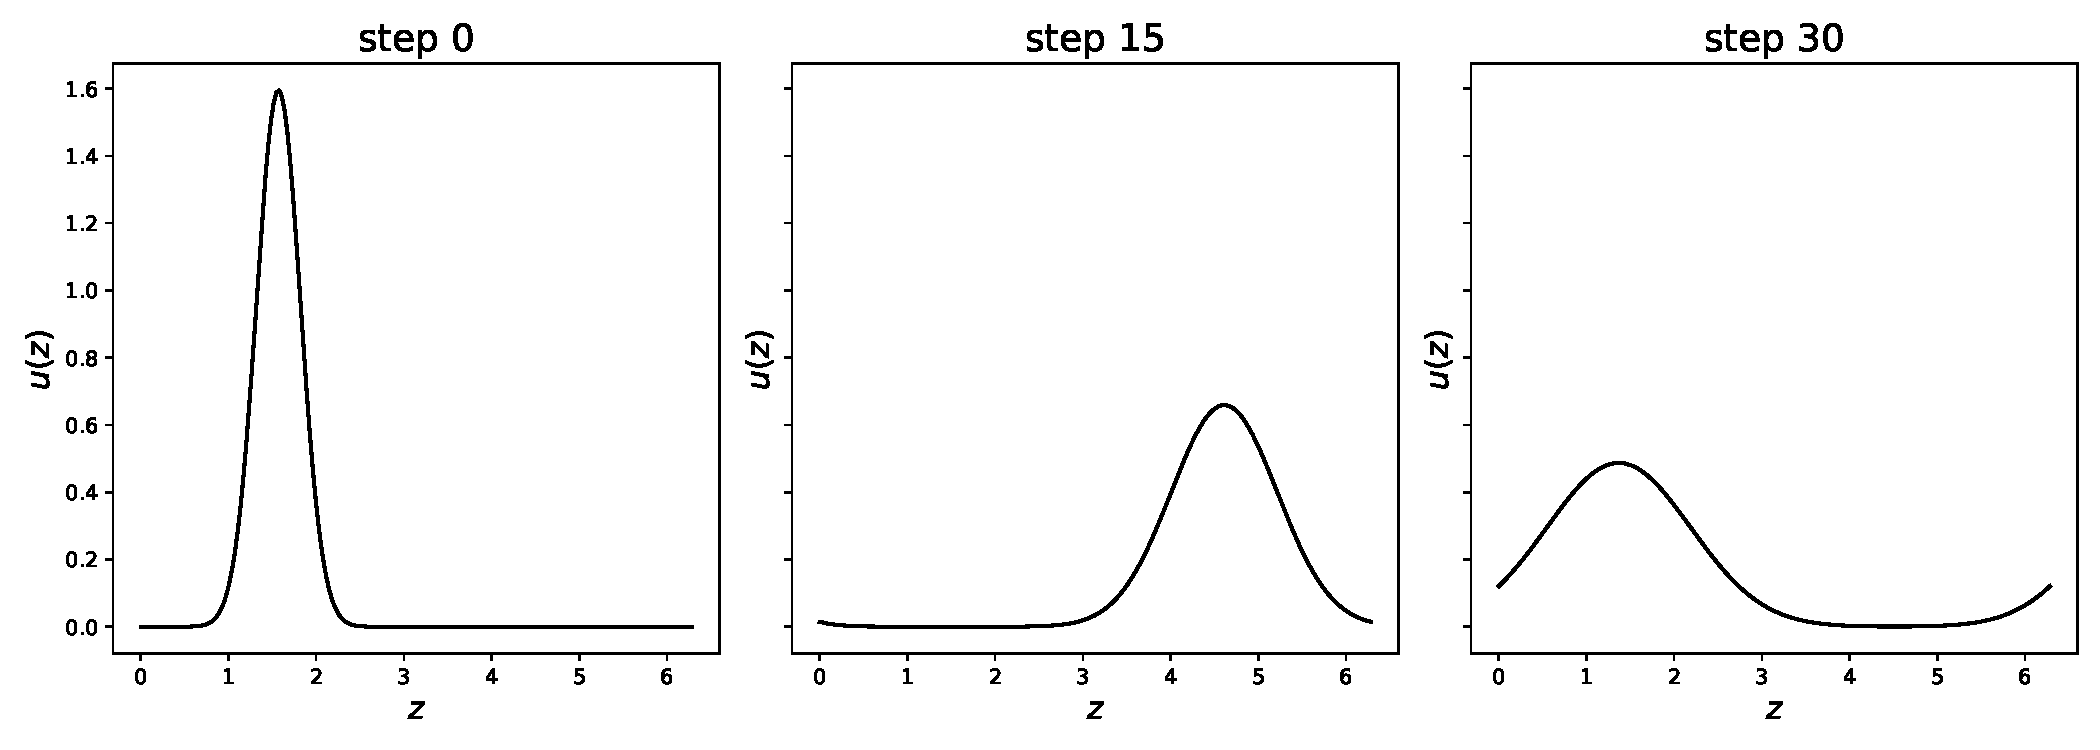
\includegraphics[width=\linewidth]{images/app1d/analytical_frame.pdf}
    \caption{La solution analytique du problème de convection-diffusion évolue au fil du temps.}
    \label{fig:1d_analytical}
\end{figure}

La forme lagrangienne des équations s'écrit

\begin{equation*}
    \frac{dx_p}{dt} = v(x_p, t), \quad \frac{dU_p}{dt} = D \frac{d^2 U_p}{dx^2}
\end{equation*}

Tout comme la méthode vortex décrite en Section~\ref{sec:vortex}, la résolution est réalisée en appliquant un schéma en deux étapes (\textit{viscous splitting}). où l'advection est réalisée au travers d'un schéma d'intégration euler explicite et l'opérateur laplacien est approché en toute position $\bx_p$ comme

\begin{equation*}
    \frac{dU_p}{dt} = D \varepsilon^{-d} V_p \sum_q (U_q - U_p) \phi_\varepsilon(x_q -  x_p),
\end{equation*}

% à mettre partie VIC
Le problème étant périodiques, nous définissons une fonction noyau équivalente $\phi_\varepsilon = \phi^P_g = \sum_{n=-\infty}^{+\infty} \phi_g(r - 2 \pi n)$.

Le modèle basé sur les particules utilise une discrétisation de \npart{} particules avec une taille de $h = \frac{L}{N_{\text{part}}}$ et une longueur de lissage de $\varepsilon = 1.3 h$.

Pour des raisons de comparaison, nous résolvons l'équation de convection-diffusion avec un schéma explicite de différences finies centrales discrétisé sur une grille régulière avec \ngrid{} nœuds.

\subsection{Paramètres d'assimilation et génération de l'ensemble}

\subsubsection{Distribution initiale}

On définit une distribution initiale pour le champ $u(\cdot, 0)$. A partir de cette distribution, un ensemble de taille  $N = 25$ membres est généré et resta commun aux différents fitres. Chaque membre par une fonction gaussienne définie par une moyenne et un écart-type différents. Egalement, les paramètres de l'équation d'évolution, la vitesse \(v\) et le coefficient de diffusion \(D\),  sont supposés inconnus. De cette manière une erreur de modèle est introduite et une calibration peut être réalisée. Les différentes distributions utilisées pour ces échantillons sont détaillées dans la Table~\ref{tab:ens_gen_1d}. Les paramètres échantillonnés et les états initiaux sont illustrés dans la Figure~\ref{fig:initial_gen}.

\begin{table}[htbp]
    \centering
    \caption{Ensemble generation variables}
    \begin{tabular}[t]{|l|l|}
        \hline
        Variables                   & Distributions                              \\
        \hline
        Gaussian mean               & $Z_m \sim  \mathcal{N}(\meanZm, \sigmaZm)$ \\
        Gaussian standard deviation & $S_m \sim\mathcal{U}(\smLow, \smUp)$       \\
        velocity                    & $v \sim \mathcal{N}(\vmean, \vstd)$        \\
        diffusion                   & $D \sim \mathcal{U}(\Dlow, \Dup)$          \\
        \hline
    \end{tabular}
    \label{tab:ens_gen_1d}
\end{table}

\begin{figure}[ht!]
    \centering
    \begin{subfigure}{0.49\textwidth}
        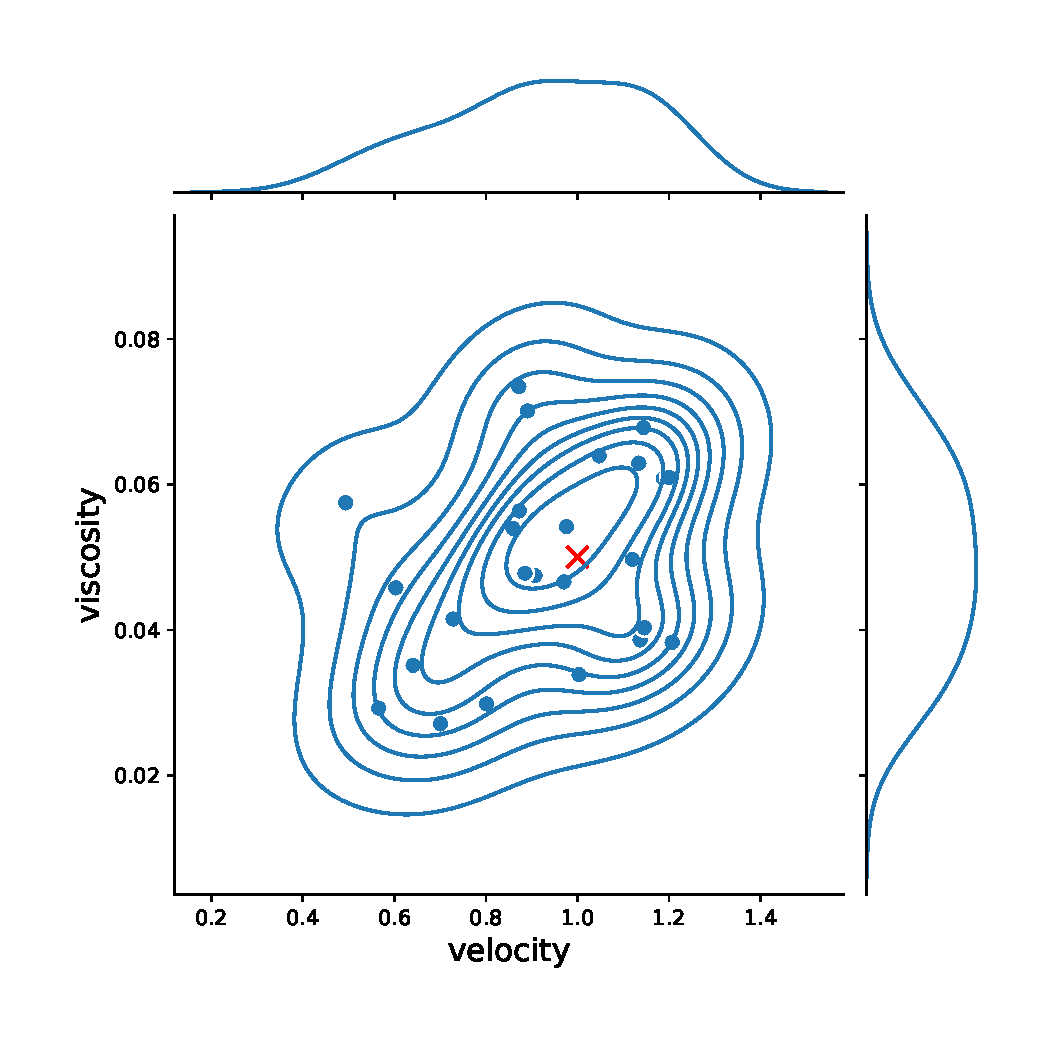
\includegraphics[width=\textwidth]{images/app1d/param.pdf}
    \end{subfigure}
    \hfill
    \begin{subfigure}{0.49\textwidth}
        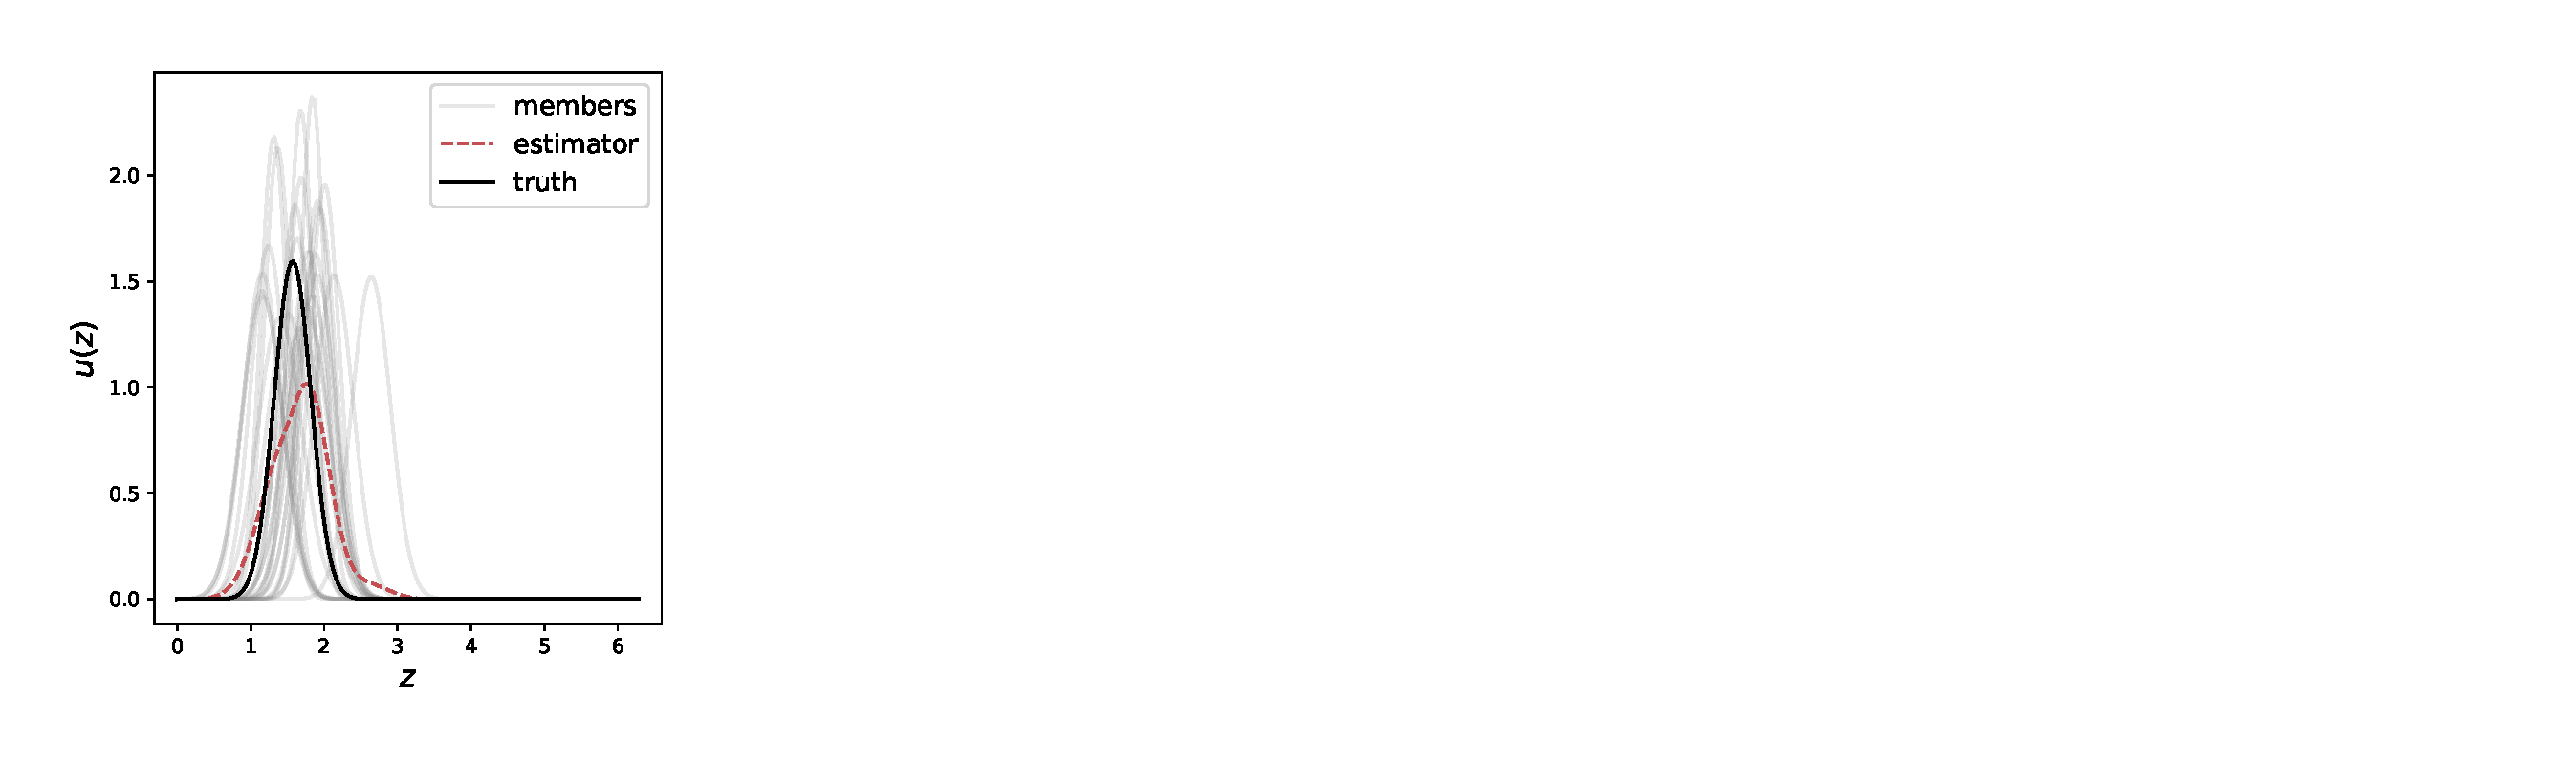
\includegraphics[width=\textwidth]{images/app1d/prior.pdf}
    \end{subfigure}
    \caption{On the left the initial parameters sample, $v$ in abscissa and $D$ in ordinate. On the right is the initial ensemble state.}
    \label{fig:initial_gen}
\end{figure}

Les données d'observation sont sujettes à un bruit additif, noté \(\eta \sim \mathcal{N}(0, \sigma_y \bm{I})\), où \(\sigma_y = \sigmaY\) et \(\bm{I}\) représente la matrice identité.

\subsubsection{Définition de l'erreur}

Nous définissons l'erreur comme le rapport relatif suivant

\begin{equation}~\label{eq:L2_error}
    e_{L_2} = \frac{\left[\frac{1}{\nens} \sum_{i = 1}^{\nens} \int_\Omega \left(u_i(z) - u^{gt}(z)\right)^2 dz\right]^{1/2}}{\norm{u^{gt}}_{L_2}}
\end{equation}
où \(u_i\) désigne le \(i\)-ème membre de l'ensemble et \(\norm{u}_{L_2}\) désigne la norme \(L_2\) de \(u^{gt}\).

La norme \(L_2\) est calculée en utilisant une quadrature sur une grille régulière d'un ensemble de cellules \(\mathcal{C}\) tel que pour tout \(f \in L_2\),

$$
    \norm{f}_{L_2} = \int_{\Omega} f^2~d\Omega \approx \sum_{c \in \mathcal{C}} f(z)~V_c
$$
où \(z_c\) est le centre de la cellule \(c\) et \(V_c\) le volume de la cellule. La grille reste la même pour toutes les simulations.

\subsubsection{Paramètres numériques}

Nous réalisons \(N_{\text{assim}} = 30\) étapes d'assimilation à intervalles réguliers jusqu'au temps final \(t_f = 2 \frac{L}{v}\). À chaque étape d'assimilation, le champ \(u^{gt}\) est observé à six positions régulièrement espacées \(x_{\text{obs}}\).

Dans la simulation basée sur des particules, les champs sont discrétisés en utilisant des particules régulièrement espacées mais avec un léger décalage. Les valeurs d'intensité sont obtenues en assignant la valeur d'intensité de particule $U_p = u(x_p) V_p$ de la même manière qu'en Section~\ref{sec:approx_part}. Cependant, le support particulaire de chaque membre sera différent. En effet, nous souhaitons évaluer notre méthode dans des situations où la discrétisation particulaire ne recouvre pas $\Omega$ dans sa totalité. Le support des particules semble déterminant pour le filtre Part-EnKF décrit en Section \ref{sec:part_enkf}. Ainsi, le paramètre \(\varepsilon_{\text{mass}}\) est introduit comme un seuil pour la sélection des particules, permettant de définir des nombres variables de particules pour chaque simulation.

Simultanément, une mise à jour standard de l'Ensemble Kalman Filter (EnKF) est appliquée aux variables nodales sur la simulation sur grille. Nous appellerons le filtre Grid-EnKF, le filtre EnKF utilisé pour la discrétisation sur grille. Pour la simulation basée sur une grille, les champs de chaque membre sont interpolés aux emplacements des nœuds. De cette manière, l'ensemble généré reste le même pour des fins de comparaison.

\subsection{Résultats}

Nous comparons les différents filtres sur l'assimilation de l'état. Nous comparons les différentes implémentation du filtre EnKF: le Grid-EnKF, le Remesh-EnKF, et deux filtres Part-EnKF avec un nombre de particules différents (100 et 60 particules). L'échantillon des paramètres reste inchangé. Nous prenons en compte les paramètres inconnus comme des incertitudes du modèle.

Dans la figure \ref{fig:1d_error_time}, nous apprécions les différentes étapes d'assimilation.

\begin{figure}
    \centering
    \begin{subfigure}{\textwidth}
        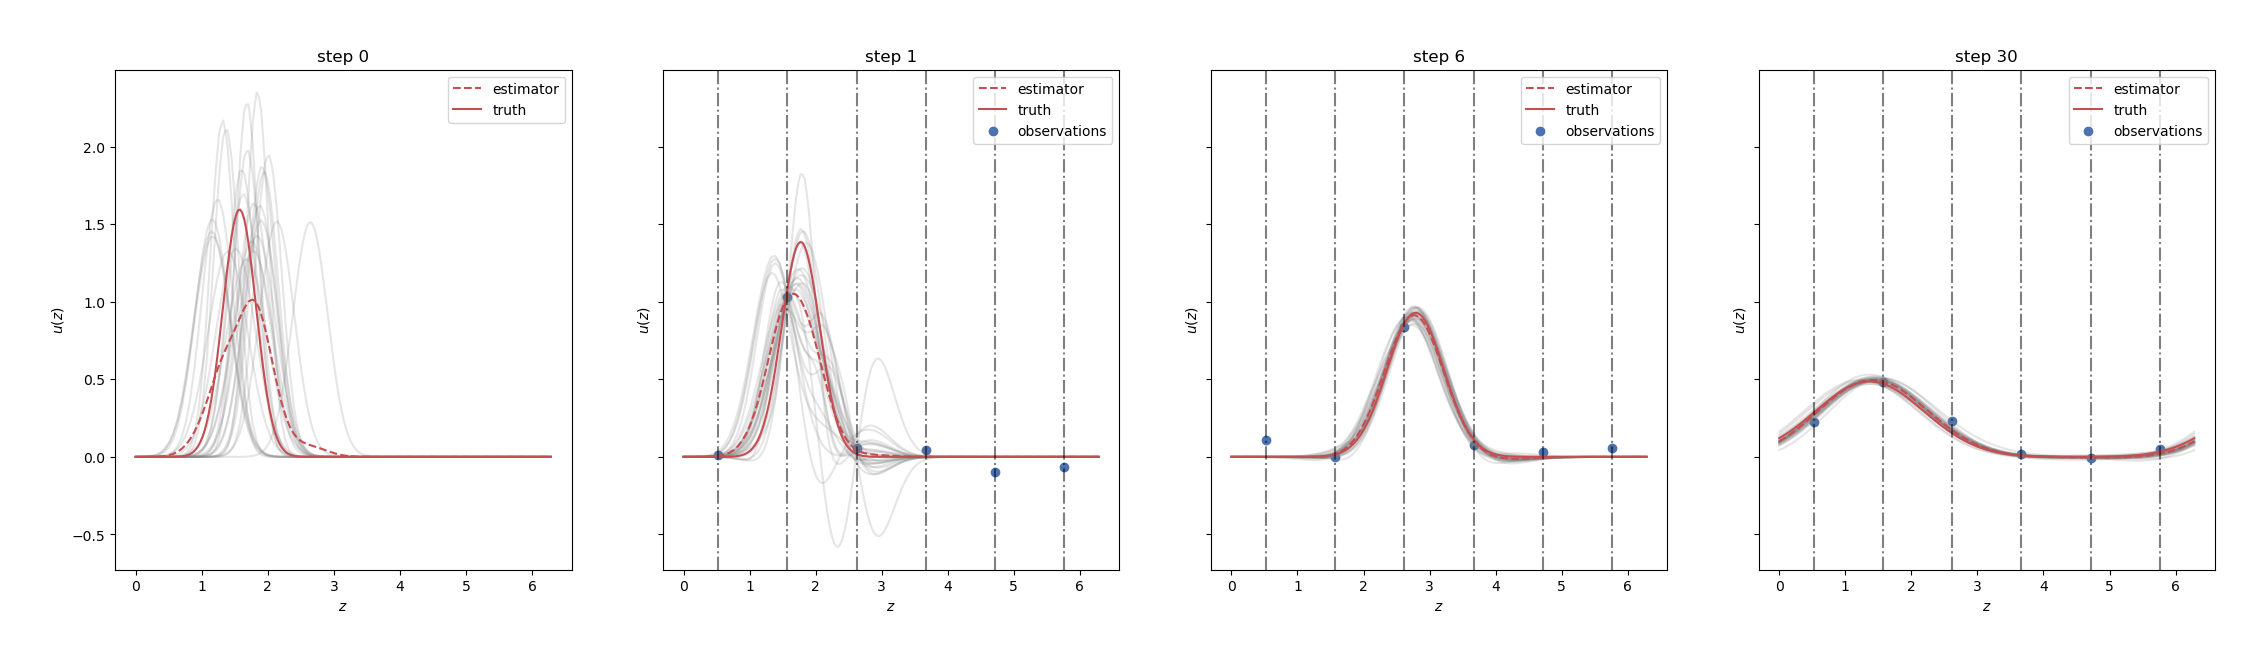
\includegraphics[width=\textwidth]{images/app1d/wo_calibration/grid_euler.png}
    \end{subfigure}
    \begin{subfigure}{\textwidth}
        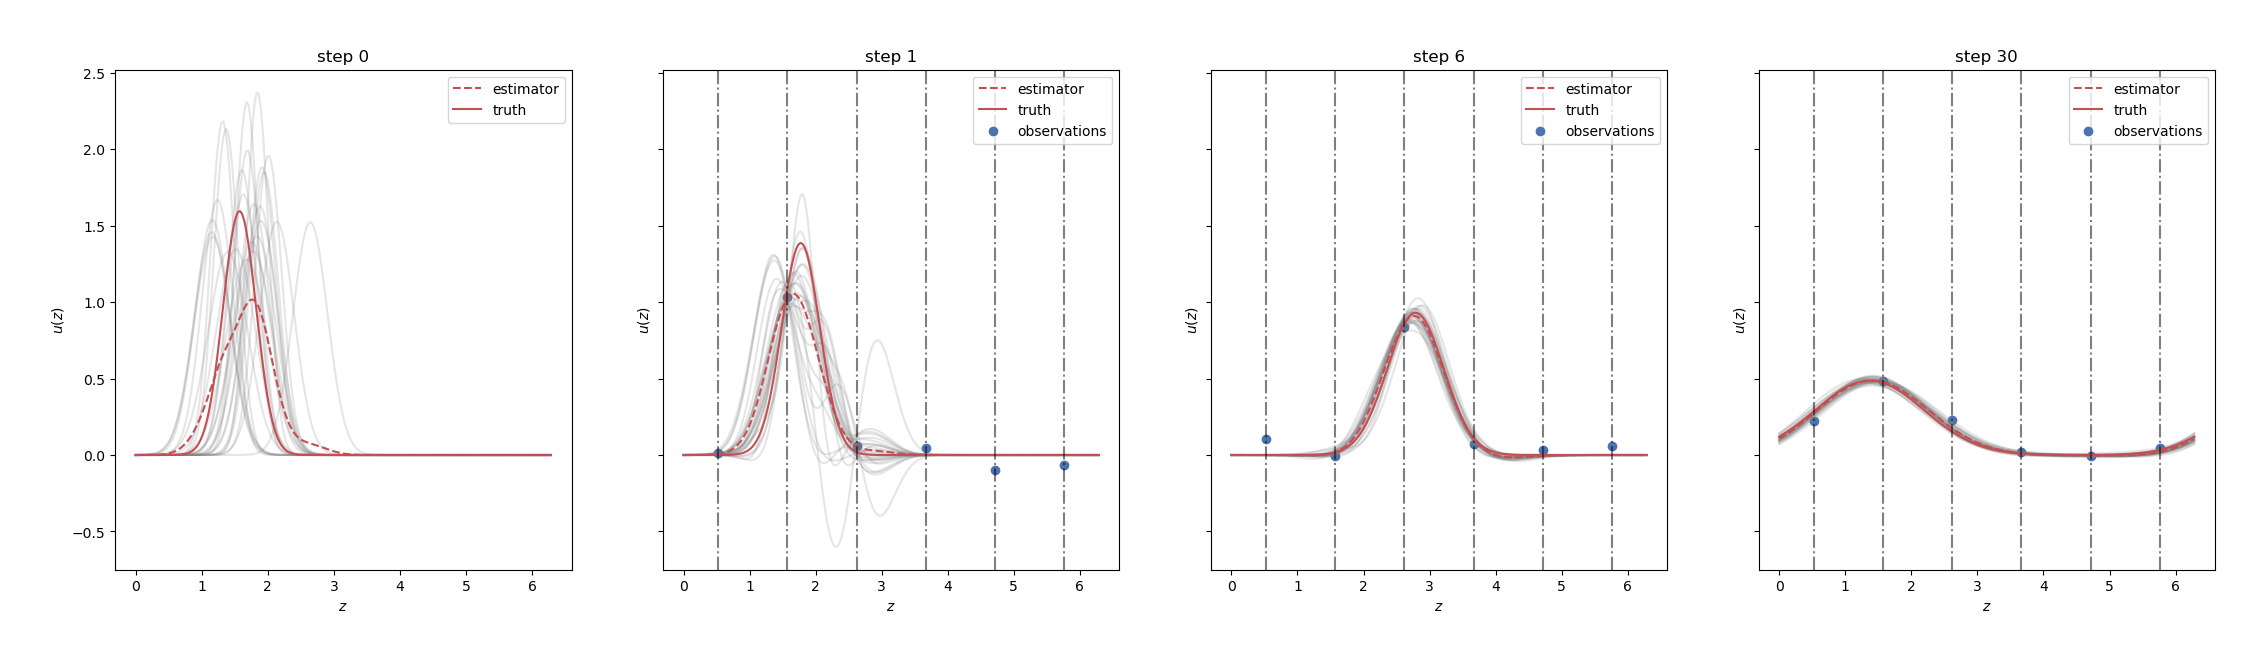
\includegraphics[width=\textwidth]{images/app1d/wo_calibration/remesh_EnKF.png}
    \end{subfigure}
    \begin{subfigure}{\textwidth}
        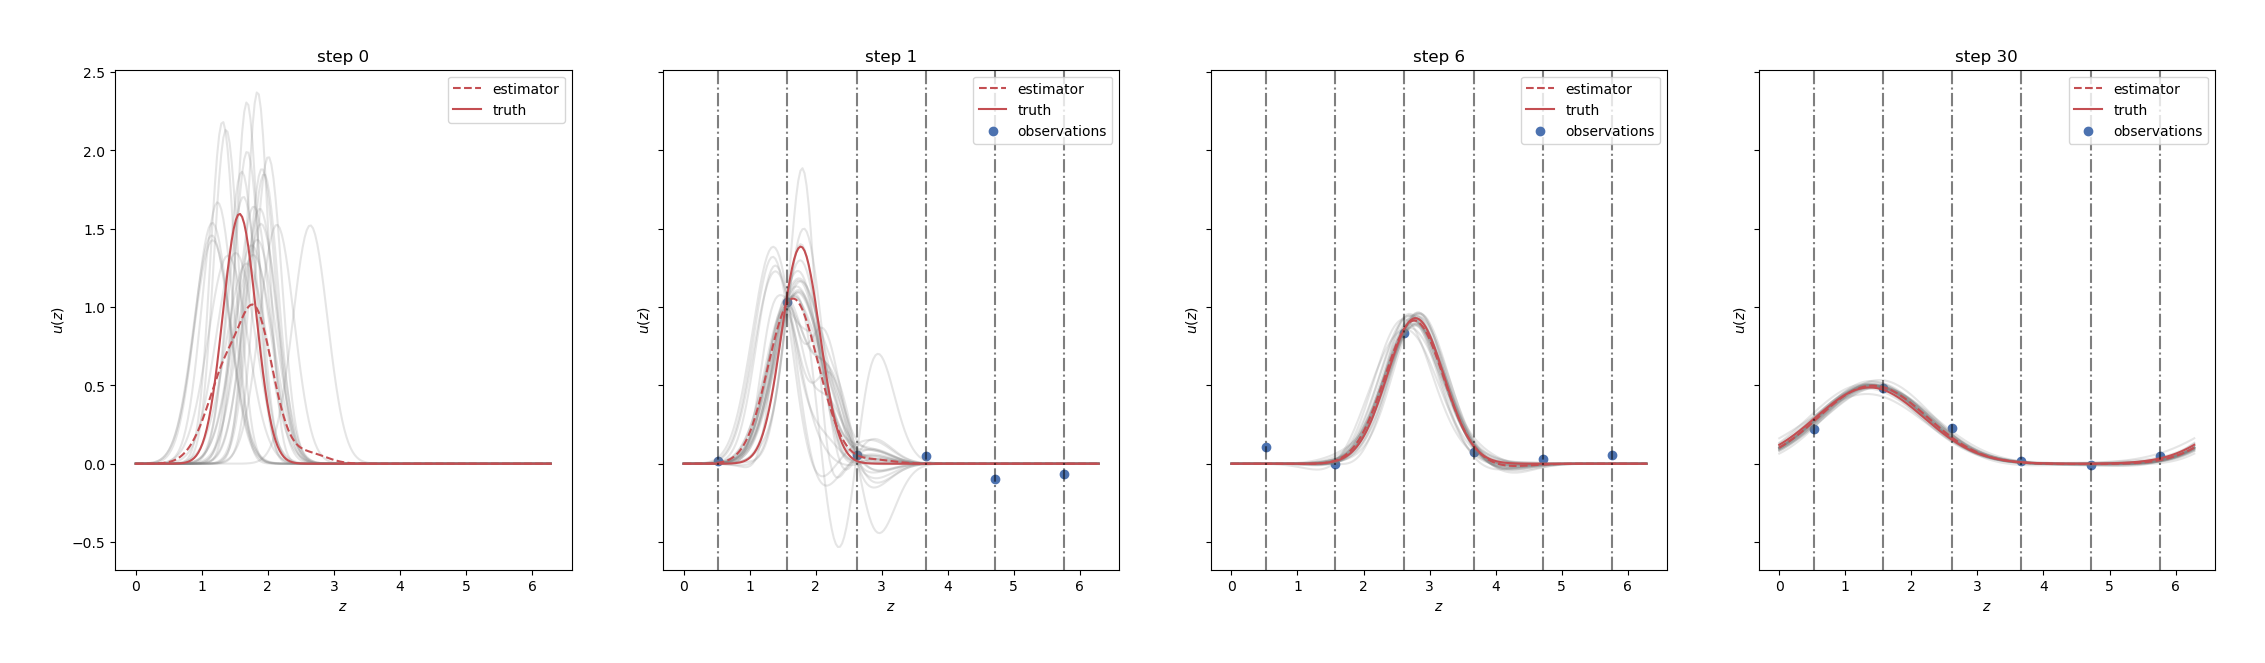
\includegraphics[width=\textwidth]{images/app1d/wo_calibration/part_enkf_30.png}
    \end{subfigure}
    \begin{subfigure}{\textwidth}
        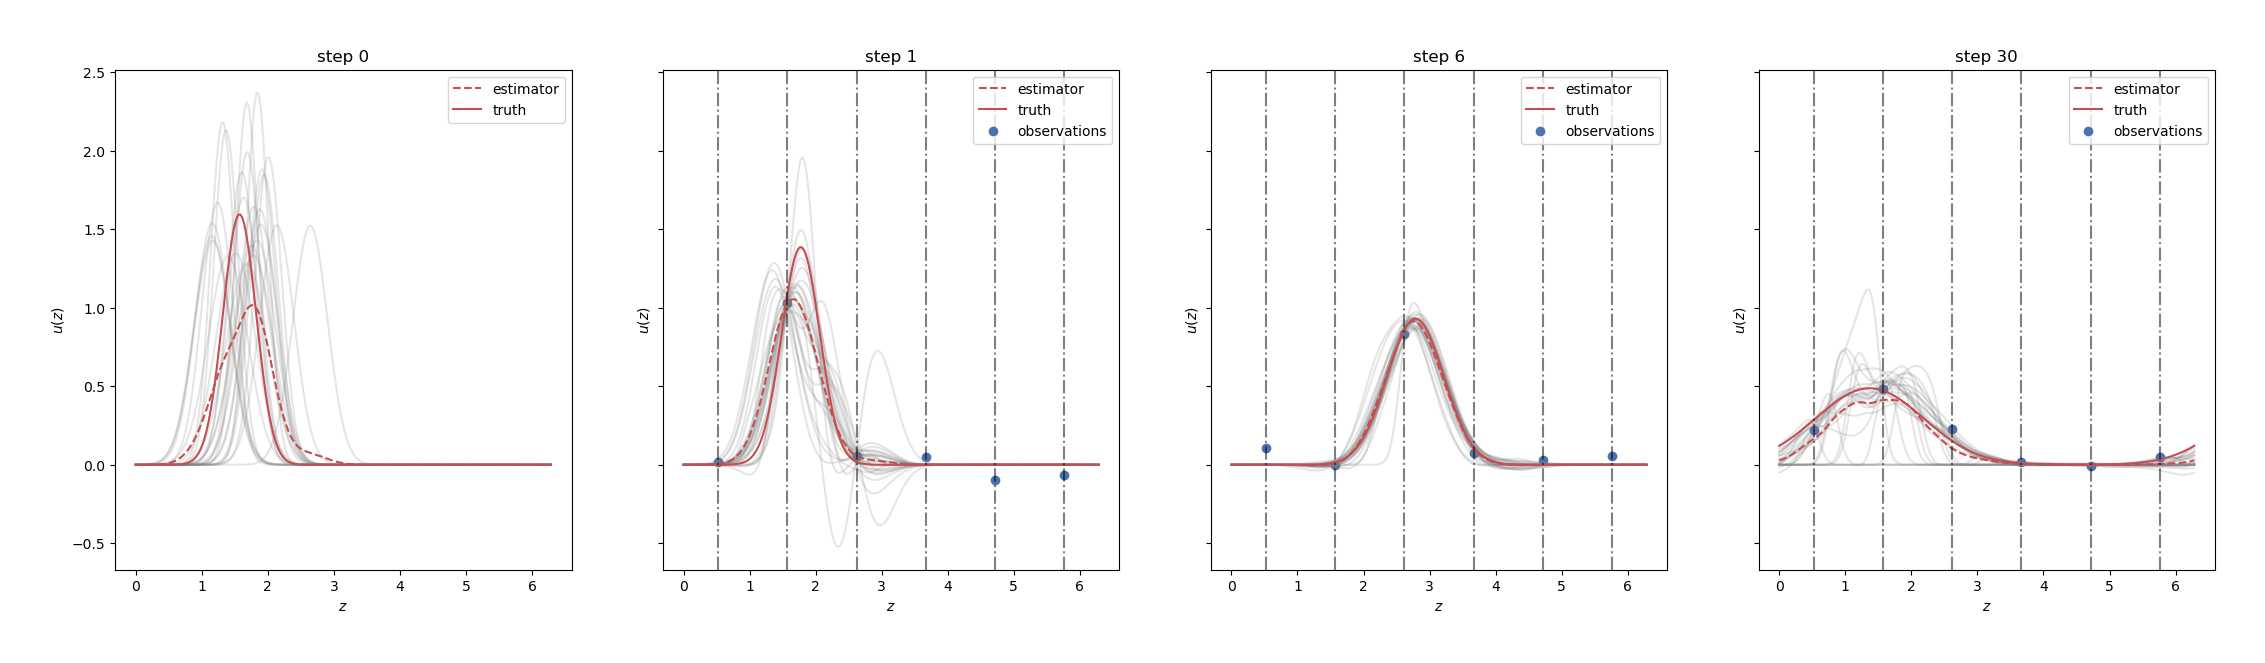
\includegraphics[width=\textwidth]{images/app1d/wo_calibration/part_enkf_60.png}
    \end{subfigure}
    \caption{Comparaison de l'assimilation des données entre différents filtres. De haut en bas : avec le filtre Grid-EnKF, le Remesh-EnKF, le Part-EnKF avec \(N_{\text{part}}=100\), et le Part-EnKF avec \(N_{\text{part}}=60\).}
\end{figure}
Le résultat est assez similaire pour tous les différents filtres. Néanmoins dans le cas où le support de particules est le plus faible, le filtre Part-EnKF avec 60 particules, le filtre ne converge pas. On retrouve quantitativement cette constatation sur la Figure~\ref{fig:1d_error_time}.

\begin{figure}
    \centering
    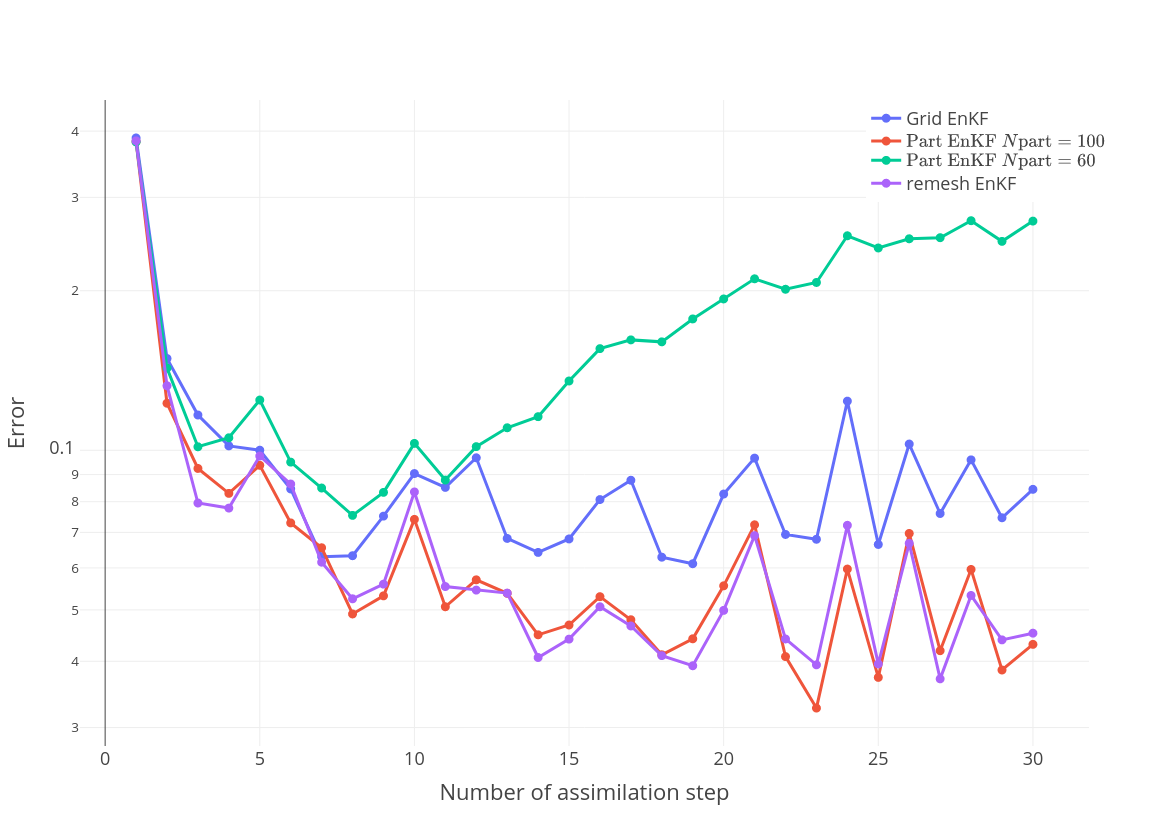
\includegraphics[width=0.75\textwidth]{images/app1d/wo_calibration/state_error.png}
    \caption{Erreur d'état en fonction du pas de temps d'assimilation.}
    \label{fig:1d_error_time}
\end{figure}

Le principal problème provient de la régression des champs analysés sur des supports de particules non conformes. Dans ce cas, la régression peine à ajuster les intensités de particule pour approcher le champ analysé définie sur un support de particules plus vaste. On observe en particulier une variabilité accrue au niveau la queue de la distribution.

Nous validons cette hypothèse en faisant varier le support initial des particules. Quantitativement, comme observé dans la Figure~\ref{fig:error_support}, l'estimation de l'erreur et la dispersion diminuent avec l'augmentation du nombre de particules. À partir de 70 particules, remarque
\begin{figure}
    \centering
    \begin{subfigure}{0.39\textwidth}
        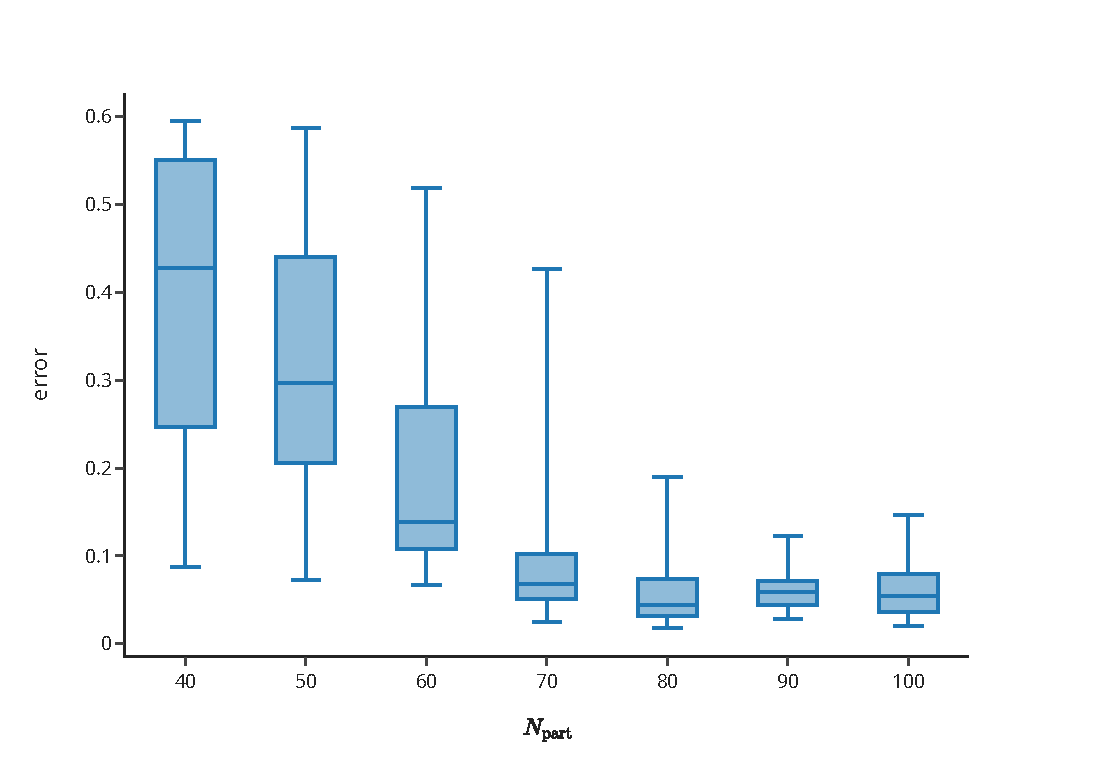
\includegraphics[width=\textwidth]{images/app1d/error_support/error_part.pdf}
        \caption{Erreur en fonction de la taille du support de particules.}
        \label{fig:error_support1}
    \end{subfigure}
    \hfill
    \begin{subfigure}{0.29\textwidth}
        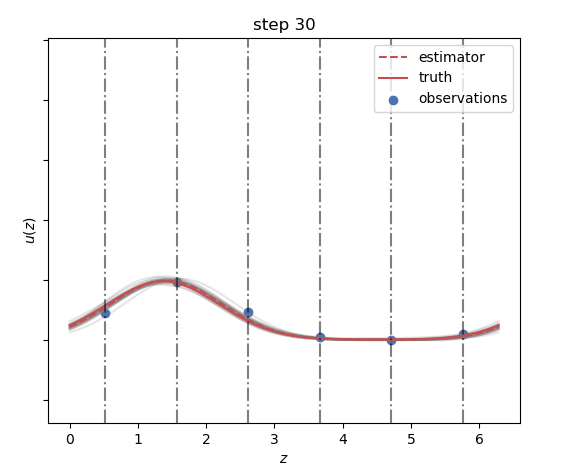
\includegraphics[width=\textwidth]{images/app1d/error_support/ok.png}
        \caption{Étape finale pour un support de 100 particules.}
        \label{fig:error_support2}
    \end{subfigure}
    \hfill
    \begin{subfigure}{0.29\textwidth}
        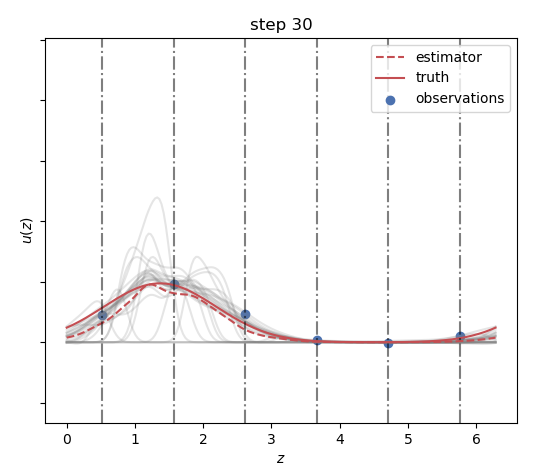
\includegraphics[width=\textwidth]{images/app1d/error_support/not_ok.png}
        \caption{Étape finale pour un support de 60 particules.}
        \label{fig:error_support3}
    \end{subfigure}
    \caption{À gauche : Erreur en fonction de la taille du support de particules. Au milieu : Étape finale pour un support de 100 particules. À droite : Étape finale pour un support de 60 particules.}
    \label{fig:error_support}
\end{figure}

Pour résoudre ce problème courant dans la régression par fonctions de base radiale (RBF)~\cite{fornberg_flyer_2015}, il est nécessaire d'augmenter le coefficient de pénalisation de la régression \textit{Ridge}.

Même avec une régression plus stable, elle reste une projection de la solution d'analyse sur le précédent jeu de particule, le seul moyen d'amélioration de la solution est donc d'ajouter des particules supplémentaires.

Cependant, l'ajout de particules reste quelque chose de complexe, pourfois même impossible. De plus, il est alors nécessaire de préserver un bon espacement entre les particules et une densité particulaire adéquate. De plus, le filtre Part-EnKF a été introduit justement pour traiter le cas où la génération de nouvelles particules ne serait pas possible.

Ainsi, si pour le filtre Part-EnKF, l'erreur de reconstruction est trop importante (par exemple en évaluant l'écart sur un nouveau jeu de particules) et si la génération de particule est possible, alors il préférable d'utiliser alors le filtre Remesh-EnKF

En conclusion, cet exemple souligne la capacité du filtre Remesh-EnKF à produire des résultats comparables à ceux de l'EnKF classique appliqué à un modèle de grille. De plus, il met en évidence la capacité du Part-EnKF à assimiler une discrétisation par particules tout en soulignant l'importance de prendre en compte la répartition spatiales des particules inter et intra membres.

\section{Problème 2D}

\subsection{Description du problème}

Dans cette section nous évaluons le résultat des deux types de filtre sur un problème bi-dimensionnel en utilisant la méthode vortex comme décrite en Section~\ref{sec:vortex}.

Nous procédons à l'assimilation du problème d'advection d'un dipôle de Lamb-Chaplygin au sein d'un domaine fermé $[0, \pi]^2$. Le dipôle de Lamb-Chaplygin est un choix populaire pour les études numériques~\cite{orlandi_vortex_1990}. Le modèle représente un écoulement dipolaire spécifique, stationnaire, offrant une solution non triviale aux équations d'Euler bidimensionnelles dans le cas non visqueux. Ce qui d'autant plus interessant est que ce dipôle est caractérisé par une vitesse de translation \(U\), une position moyenne \(\bm{z}_0\), un rayon \(R\) et une orientation \(\alpha\).

Le champ de vorticité du dipôle \(\omega\) peut être exprimé comme

\begin{equation*}
    \omega(r) = \begin{cases}
        \frac{-2 k U J_1(kr)}{\omega J_0(kR)} \sin \alpha \quad & \text{pour} \quad r < R, \\
        0 \quad                                                 & \text{sinon},
    \end{cases}
\end{equation*}
où \((r, \alpha)\) représentent les coordonnées polaires dans le référentiel du dipôle. Ici, \(J_0\) et \(J_1\) désignent respectivement les fonctions de Bessel de premier type d'ordre zéro et d'ordre un, et \(k\) est déterminé de sorte que \(kR\) corresponde au premier zéro non trivial de la première fonction de Bessel. Le champ de vorticité du dipôle est illustré dans la Figure \ref{fig:lamb_dipole}.

\begin{figure}[ht]
    \centering
    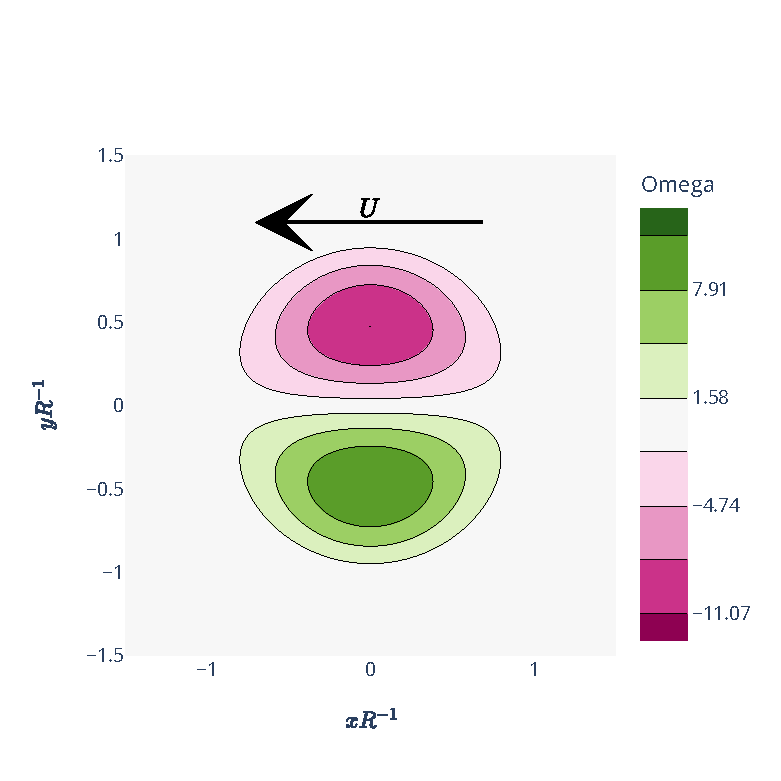
\includegraphics[width=0.6\linewidth]{images/app2d/lamb.pdf}
    \caption{The Lamb-Chaplygin dipole vorticity field on a normalized space.}
    \label{fig:lamb_dipole}
\end{figure}

Le dipole est initialement positionné au centre du domaine avec une orientation de \(\frac{7\pi}{8}\) rad, un rayon de 0.5m et une vitesse \(U\) de 0.25 \(\text{m.s}^{-1}\). Les paramètres de référence complets sont listés dans le Tableau \ref{tab:ref}.

\begin{table}[htbp]
    \centering
    \caption{Paramètres de référence}
    \begin{tabular}[t]{|l|l|}
        \hline
        Paramètres               & Valeurs                                                              \\
        \hline
        viscosité de référence   & $v_{\text{ref}} = 0.001$                                             \\
        orientation de référence & $\theta_{\text{ref}}  = \frac{7 \pi}{8} (\text{rad.})$               \\
        position du barycentre   & $\bm{z}_{\text{ref}} = \left[\frac{\pi}{2}, \frac{\pi}{2} \right]^T$ \\
        vitesse de translation   & $U_{\text{ref}} = 0.25$                                              \\
        \hline
    \end{tabular}
    \label{tab:ref}
\end{table}

Aux frontières, la vitesse normale aux parois est nulle, tandis que la vitesse tangentielle reste indéterminée.

Comme ce problème n'a pas de solution explicite dans un domaine fermé, nous simulons la vérité terrain avec la méthode des vortex pour une discrétisation fine et un ensemble de paramètres fixes également décrits dans le Tableau \ref{tab:ref}. La trajectoire de la vérité terrain est illustrée dans la Figure \ref{fig:ref_trajectory} sur une grille régulièrement espacée.

\begin{table}[htbp]
    \centering
    \caption{Paramètres nominaux d'assimilation et de simulation}
    \begin{tabular}[t]{|l|l|}
        \hline
        Paramètres                              & Valeurs                                     \\
        \hline
        pas de temps                            & $dt = 0.005$                                \\
        temps final                             & $t_f = 10$                                  \\
        écart-type de l'observation             & $\sigma_{obs} =  5.0 \times 10^{-2}$        \\
        seuil de vorticité                      & $\varepsilon_{\omega} = 1.0 \times 10^{-4}$ \\
        longueur caractéristique des particules & $dp = \frac{\pi}{256} \approx 0.01227 $     \\
        longueur de lissage                     & $h = 2.0 \, dp$                             \\
        nombre d'assimilations                  & $N_{\text{assim}} = 10$                     \\
        taille de l'ensemble                    & $N_{\text{ens}} = 32$                       \\
        nombre d'observations                   & $N_{\text{obs}} = 12^2 = 144$               \\
        discrétisation de la grille             & $N_{\text{grid}} = 65^2 = 4225$             \\
        % nombre de remaillages par prévision     & $N_{\text{remesh}} = 2 $                    \\
        \hline
    \end{tabular}
    \label{tab:simu_2d}
\end{table}

\begin{figure}[htbp]
    \begin{subfigure}{0.32\textwidth}
        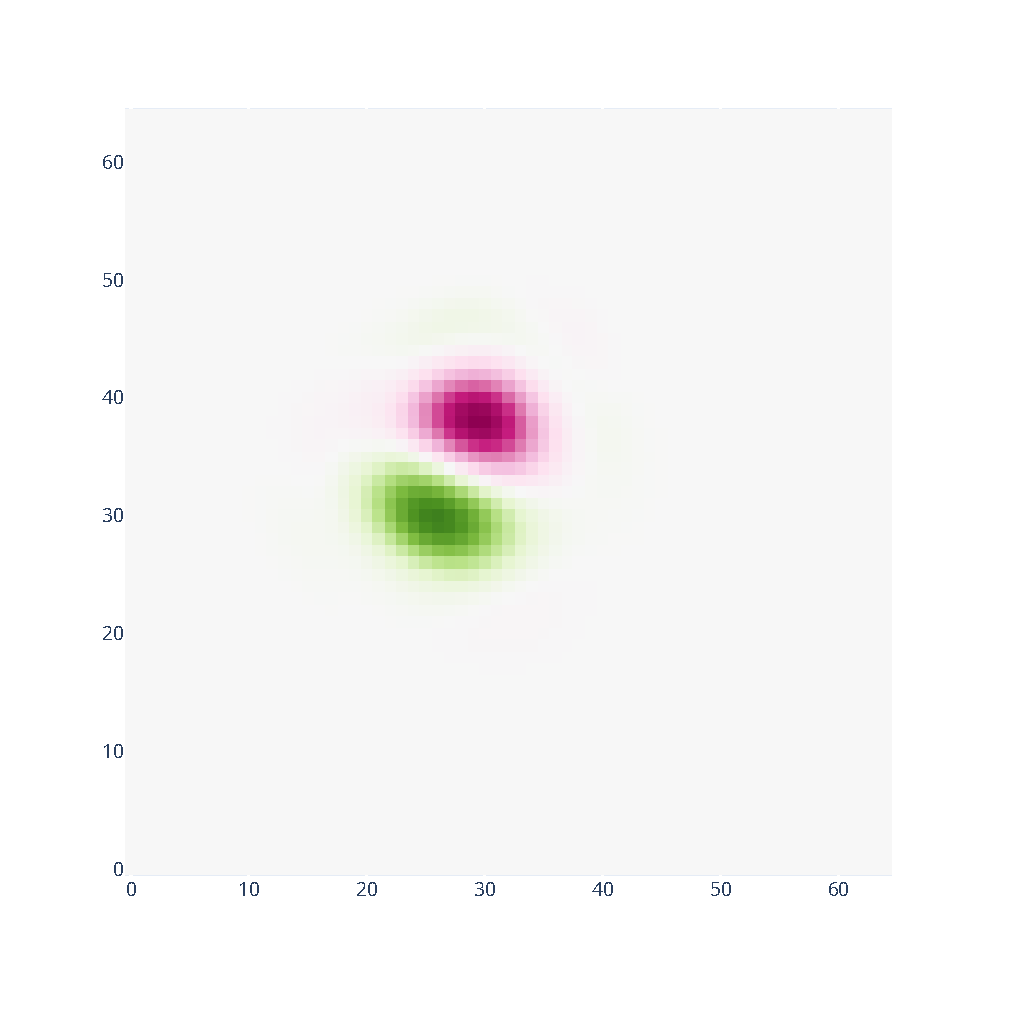
\includegraphics[width=\linewidth]{images/app2d/best_estimate_2.pdf}
    \end{subfigure}
    \hfill
    \begin{subfigure}{0.32\textwidth}
        \includegraphics[width=\linewidth]{images/app2d/best_estimate_10.pdf}
    \end{subfigure}
    \hfill
    \begin{subfigure}{0.32\textwidth}
        \includegraphics[width=\linewidth]{images/app2d/best_estimate_20.pdf}
    \end{subfigure}
    \caption{Trajectoire de la vérité terrain. La vorticité est représentée sur une grille régulièrement espacée. Pour $t=[1, 5, 10]$ s.}
    \label{fig:ref_trajectory}
\end{figure}


Plusieurs paramètres de la simulation influencent la distribution des particules et peuvent conduire à des résultats différents. Le premier est la taille des particules définie par \(d_p\). Un autre paramètre significatif est \(\varepsilon_\omega\), associé au processus de remaillage se produisant soit pendant la prévision (pour éviter une distorsion élevée de la distribution des particules) soit pendant le filtre Remesh-EnKF. \(\varepsilon_\omega\) sert de seuil, déterminant si une particule est retenue après le processus de remaillage basé sur la condition \(V_p \Gamma_p > \varepsilon_\omega\). L'impact de ce paramètre est illustré pour un membre après la première prévision dans la Figure~\ref{fig:eps_effect}.

\begin{figure}[htbp]
    \centering
    \begin{subfigure}{0.3\textwidth}
        \includegraphics[width=\linewidth]{images/app2d/part_eps_0.1.png}
    \end{subfigure}
    \hfill
    \begin{subfigure}{0.3\textwidth}
        \includegraphics[width=\linewidth]{images/app2d/part_eps_0.01.png}
    \end{subfigure}
    \hfill
    \begin{subfigure}{0.3\textwidth}
        \includegraphics[width=\linewidth]{images/app2d/part_eps_1e-6.png}
    \end{subfigure}
    \caption{Effet du paramètre $\varepsilon_\omega$ sur la discrétisation des particules de la solution pour un membre. De gauche à droite, résultats pour $\varepsilon_\omega = 0.1, 0.01$ et $1.e^{-6}$.}
    \label{fig:eps_effect}
\end{figure}


\subsection{Paramètres d'assimilation et génération d'ensemble}

\subsubsection{Distribution d'ensemble}
Nous générons un ensemble initial de 32 membres en échantillonant une distribution de paramètre du dipole.

Nous échantillonnons le rayon \(R\), la vitesse prescrite \(U\), l'orientation \(\alpha\) et le barycentre \(\bm{z}_{\text{mean}}\). De plus, la viscosité du modèle \(\nu\) est également échantillonnée. Toutes les distributions sont résumées dans le Tableau \ref{tab:ens_dipole}. Les six premiers membres sont représentés dans la Figure \ref{fig:sample_ens}.

\begin{table}[htbp]
    \centering
    \caption{Variables de génération de l'ensemble}
    \begin{tabular}[t]{|l|l|}
        \hline
        Variables   & Distributions                                                                                                                                  \\
        \hline
        rayon       & $R \sim \mathcal{N}(1.0, 0.05^2)$                                                                                                              \\
        orientation & $\theta \sim \mathcal{U}\left(\pi, \frac{\pi}{2} \right) (\text{rad.})$                                                                        \\
        barycentre  & $z_{\text{mean},x} \sim \mathcal{N}\left(\frac{\pi}{2},0.1^2\right), \quad z_{\text{mean},y} \sim \mathcal{N}\left(\frac{\pi}{2},0.1^2\right)$ \\
        vitesse     & $U \sim \mathcal{U}(0, 0.5^2)$                                                                                                                 \\
        viscosité   & $v \sim \mathcal{N}(0.0015, 0.0005^2)$                                                                                                         \\
        \hline
    \end{tabular}
    \label{tab:ens_dipole}
\end{table}

\begin{figure}[ht]
    \centering
    \includegraphics[width=0.9\linewidth]{images/app2d/ensemble_sample.png}
    \caption{Six échantillons de l'ensemble initial.}
    \label{fig:sample_ens}
\end{figure}

Le champ de vorticité initial est d'abord discrétisé sur une grille régulière de particules avec une longueur caractéristique \(d_p\), où chaque particule reçoit la circulation \(\Gamma_p = \omega(\bm{z}_p) V_p\) et \(V_p = d_p^2\) représente le volume de la particule.

\subsubsection{Définition de l'erreur}

Nous utilisons une erreur absolue \(L_2\) définie par $ \frac{1}{\nens} \sum_{i = 1}^{\nens} \int_\Omega \left(\omega_i(\bm{z}) - \omega^{gt}(\bm{z})\right)^2 \mathrm{d}\bm{z}$. Nous utilisons également les erreurs des membres pour évaluer la dispersion de l'estimation de l'erreur.

\subsubsection{Paramètres numériques}

La fréquence d'assimilation est définie par le pas d'assimilation $dt_a$. La simulation est effectuée sur une durée de $t_f$. Tous les paramètres de simulation sont résumés dans le Tableau \ref{tab:simu_2d}.

Les observations sont collectées sur une grille régulière de taille $N_{\text{obs}}$, mesurant les deux composantes de la vitesse. Les observations suivent une distribution normale $\mathcal{N}(0, \sigma_{\text{obs}}^2 \bm{I})$, indiquant un ensemble de mesures indépendantes, chacune caractérisée par une distribution standard de $\sigma_{\text{obs}}$. Un exemple de vitesse observée avec et sans bruit est illustré dans la Figure \ref{fig:velocity}.

\begin{figure}[htbp]
    \centering
    \includegraphics[width=0.8\linewidth]{images/app2d/velocity_ref_recadre.pdf}
    \caption{Champs de vitesse observés et de référence. L'erreur sur chaque composante est un échantillon d'une distribution normale centrée avec la valeur nominale $\sigma_{\text{obs}} = 0.05$.}
    \label{fig:velocity}
\end{figure}

\subsection{Résultats}

\subsection{Assimilation au cours du temps}

Nous commençons par analyser l'erreur d'assimilation au cours du temps. La Figure~\ref{fig:assim_time} illustre l'erreur tout au long du processus d'assimilation pour l'ensemble nominal de paramètres d'assimilation, montrant des résultats comparables pour les deux filtres. À chaque étape d'assimilation, l'erreur diminue sans observer de divergence dans ce cas.

\begin{figure}[htbp]
    \centering
    \includegraphics*[width=0.7\linewidth]{images/app2d/final/error_in_time.pdf}
    \caption{Courbes d'erreur au fil des étapes d'assimilation. À gauche : \(L_2\)-erreur du champ, À droite : Erreur pour le paramètre de viscosité. En bleu pour Part-EnKF et en rouge pour Remesh-EnKF.}
    \label{fig:assim_time}
\end{figure}

\subsubsection{Erreur par rapport aux paramètres d'assimilation}

Nous évaluons également les performances des différents filtres en évaluant la convergence de l'erreur par rapport aux paramètres d'assimilation.

Nous observons le taux de convergence par rapport aux paramètres d'assimilation : la précision des observations, qui est \(1/\sigma_{\text{obs}}^2\), le nombre d'observations \(N_{\text{obs}}\), et le nombre d'étapes d'assimilation \(N_{\text{assim}}\).

La Figure~\ref{fig:obs_precision_1} illustre une diminution du biais et des variances de l'erreur par rapport à la précision des observations, de manière similaire pour les deux filtres. Ce qui est remarquable dans la Figure~\ref{fig:obs_precision_2}, où l'échelle est logarithmique, est la régularité du taux de convergence pour les deux filtres par rapport à la précision des observations. L'ordre de convergence est d'environ 0.68 pour Part-EnKF et 0.75 pour Remesh-EnKF.

\begin{figure}[h!]
    \centering
    \begin{subfigure}{0.49\linewidth}
        \centering
        \includegraphics[width=\linewidth]{./images/app2d/final/MSE_obs_precision_box.pdf}
        \caption{}
        \label{fig:obs_precision_1}
    \end{subfigure}
    \begin{subfigure}{0.49\linewidth}
        \centering
        \includegraphics[width=\linewidth]{./images/app2d/final/MSE_obs_precision_box_log.pdf}
        \caption{}
        \label{fig:obs_precision_2}
    \end{subfigure}
    \caption{Diagrammes en boîte de l'erreur d'état en fonction de \(1/\sigma_{\text{obs}}^2\).}
\end{figure}


Dans la Figure~\ref{fig:na_1}, la réduction de l'erreur est encore notable et montre une diminution de la variance à mesure que le nombre d'observations augmente. Dans la Figure~\ref{fig:na_2} en échelle logarithmique, la diminution de l'erreur se produit également à un rythme constant pour les deux filtres. On observe un ordre de convergence plus élevé, environ 1.8 pour le Remesh-EnKF comparé à environ 1.4 pour le Part-EnKF.

\begin{figure}[h!]
    \centering
    \begin{subfigure}{0.49\linewidth}
        \centering
        \includegraphics[width=\linewidth]{./images/app2d/final/MSE_na_box.pdf}
        \caption{}
        \label{fig:na_1}
    \end{subfigure}
    \begin{subfigure}{0.49\linewidth}
        \centering
        \includegraphics[width=\linewidth]{./images/app2d/final/MSE_na_box_log_log.pdf}
        \caption{}
        \label{fig:na_2}
    \end{subfigure}
    \caption{Boîte à moustaches de l'erreur d'état en fonction de $N_{\text{assim}}$.}
    \label{fig:na}
\end{figure}

Enfin, nous analysons la convergence de l'erreur en fonction du nombre d'observations. Les emplacements des observations augmentent régulièrement sur les deux axes. Dans la Figure~\ref{fig:nobs_1}, l'estimation de l'erreur et les variances diminuent. Pour un nombre relativement faible d'observations, les deux filtres offrent des résultats similaires, tandis que le Remesh-EnKF montre des résultats relativement meilleurs lorsque le nombre d'observations est augmenté. De plus, le taux de convergence semble changer autour de 200 points d'observation, comme illustré dans la Figure~\ref{fig:nobs_2} en échelle logarithmique. Néanmoins, cela montre des performances adéquates pour les deux filtres.

\begin{figure}[h!]
    \centering
    \begin{subfigure}{0.49\linewidth}
        \centering
        \includegraphics[width=\linewidth]{./images/app2d/final/MSE_nobs_box.pdf}
        \caption{Boîte à moustaches de l'erreur d'état par rapport à $N_{\text{obs}}$.}
        \label{fig:nobs_1}
    \end{subfigure}
    \begin{subfigure}{0.49\linewidth}
        \centering
        \includegraphics[width=\linewidth]{./images/app2d/final/MSE_nobs_box_log_log.pdf}
        \caption{Boîte à moustaches de l'erreur d'état par rapport à $N_{\text{obs}}$.}
        \label{fig:nobs_2}
    \end{subfigure}
    \caption{Convergence de l'erreur par rapport au nombre d'observations. À gauche : Échelle linéaire, À droite : Échelle logarithmique.}
    \label{fig:nobs}
\end{figure}

\subsubsection{Erreur en fonction des paramètres de simulation}

Examinons maintenant l'évolution de l'erreur par rapport aux paramètres de discrétisation particulaire. En effet, pour le Part-EnKF il faut se rappeler que chaque membre a sa propre discrétisation particulaire évlouant au cours du temps. Les résultats de se filtre sont alors plus sensibles que les autres à ces paramètres.

Nous avons testé le filtre Part-EnKF en utilisant l'approximation présentée en Section~\ref{sec:approx_part} pour sa stabilité et sa rapidité lors de la mise à jour. En raison de l'irrégularité des particules dans la distribution, une approximation sévère est introduite, entraînant des erreurs entre la solution analysée et la solution approchée. De plus, qualitativement, on peut observer que certaines parties de la solution ne peuvent pas être représentée car aucune particule dans le support ne peut les interpoler. Cet effet peut être observé sur plusieurs échantillons de l'ensemble où l'analyse est projetée sur une discrétisation de particules non conforme.
Par exemple, qualitativement, nous observons la première étape d'assimilation d'un membre pour les différents filtres en Figure~\ref{fig:assim_member}. Nous constatons que la solution Part-EnKF n'est qu'une projection partielle de la même solution que Remesh-EnKF avec de plus certaines distortions.

\begin{figure}
    \centering
    \begin{subfigure}{0.32\textwidth}
        \centering
        \includegraphics[width=\linewidth]{./images/app2d/assim_member_forecast.png}
        \caption{Discrétisation des prévisions des membres.}
    \end{subfigure}
    \hfill
    \begin{subfigure}{0.32\textwidth}
        \centering
        \includegraphics[width=\linewidth]{./images/app2d/assim_member_ppf.png}
        \caption{Discrétisation de l'analyse Part-EnKF.}
    \end{subfigure}
    \hfill
    \begin{subfigure}{0.32\textwidth}
        \centering
        \includegraphics[width=\linewidth]{./images/app2d/assim_member_rmf.png}
        \caption{Discrétisation de l'analyse Remesh-EnKF.}
    \end{subfigure}
    \caption{Assimilation d'un membre avec une discrétisation des prévisions non adaptée à la solution d'analyse. La discrétisation des prévisions utilisée par le Part-EnKF ne permet pas toujours une approximation pour les analyses et introduit des erreurs de discrétisation.}
    \label{fig:assim_member}
\end{figure}

Ces remarques sont d'autant plus critiques que lorsque l'étape de \textit{forecast} est longue ou lorsque la taille du support de l'ensemble des particules est plus petite. De plus, l'approximation de la Section~\ref{sec:approx_part} introduira l'erreur d'approximation en fonction de la taille des particules à cause de l'erreur de quadrature.


Quantitativement, pour évaluer évaluer l'effet de la taille du support, nous avons fait varier la valeur de $\varepsilon_{\omega}$, valeur de seuillage sur la distribution de particules initiales. Nous avons observé sur la Figure~\ref{fig:eps_effect} que ce paramètre affecte le nombre de particules et, par conséquent, la taille du support. Dans la Figure~\ref{fig:cuttoff}, nous remarquons de grandes disparités entre les deux filtres. Cependant, l'erreur se stabilise rapidement en diminuant le seuil. Ces résultats suggèrent un impact du seuillage, donc, sur le support des particules en particulier pour le Part-EnKF. En revanche, le Remesh-EnKF est moins sensible à ce paramètre. En effet, le seuillage ne fait que retirer des particules de faible intensité sur le bord du dipole et n'influence à aucun moment la solution analysée sur des zones à forte intensité.

\begin{figure}[h!]
    \centering

    \begin{subfigure}{0.48\textwidth}
        \centering
        \includegraphics[width=\linewidth]{./images/app2d/final/MSE_cutoff_box.pdf}
        \caption{Erreur d'état par rapport à $\varepsilon_{\omega}$. Les seuils élevés, bas et moyens correspondent respectivement à $\varepsilon_{\omega} = 0.1, 1.e^{-6}$ et $0.01$.}
        \label{fig:cuttoff}
    \end{subfigure}
    \hfill
    \begin{subfigure}{0.48\textwidth}
        \centering
        \includegraphics[width=\linewidth]{./images/app2d/final/MSE_size_box.pdf}
        \caption{Erreur d'état par rapport à $d_p$. Les tailles grandes, moyennes et petites correspondent à $d_p = 0.0327, 0.0245$ et $0.0123$.}
        \label{fig:np}
    \end{subfigure}

    \caption{Boîte à moustaches des erreurs pour les paramètres de simulation. L'effet de $\varepsilon_{\omega}$ sur l'erreur est particulièrement observé pour des valeurs élevées. L'erreur du Part-EnKF est fortement liée à $d_p$ à travers l'erreur d'approximation des particules.}
    \label{fig:simu_parameters_error}
\end{figure}

Un autre paramètre déterminant pour l'assimilation est la taille de particules $d_p$. Dans la Figure~\ref{fig:np}, nous observons que l'erreur pour le filtre Part-EnKF augmente significativement avec ce paramètre. En fait, celle-ci augmente proportionnellement avec $d_p$ tout comme pour l'erreur d'approximation. Cette erreur élevée l'effet important de l'approximation des particules pour le Part-EnKF. En revanche, l'erreur pour le filtre Remesh-EnKF est relativement faible, profitant d'un schéma d'interpolation par projection d'ordre élevé comme défini en Section~\ref{sec:remesh}. L'utilisation d'un opérateur de régression ppur approximer la solution analysée devrait pouvoir atténuer cet effet, sous réserve d'autres considérations de discrétisation des particules (distorsion, taille du support) comme illustré dans la Partie~\ref{sec:App_1D} et du choix d'un coefficient de pénalité adéquat pour réussir à approximer la solution.

Finalement, cette discussion montre la grande dépendance du filter Part-EnKF vis-à-vis des paramètres de discrétisation particulaire. D'une part, la discrétisation d'un membre peut être trop éloigné de la solution à approcher.
Même si le filtre Remesh-EnKF offre lui des performances de convergence satisfaisant rappelons que c'est toujours au prix d'une nouvelle génération de particules, là où le filtre Part-EnKF offre la possibilité d'appliquer une mise à jour sans cette étape intermédiaire.

Néanmoins, cela ouvre la question du choix ou de la modification de la discrétisation des particules.

Dans le cas où la génération d'un jeu de particules régulier est possible, comme suggéré dans la Partie~\ref{sec:App_1D}, une estimation de l'erreur pourrait être introduite pour choisir entre les différents filtres. D'autre part, d'autres approches pourraient consister à sélectionner le membre de maximum de vraisemblance pour selectionner son jeu de particules pour approcher la solution analysée de tous les membres. Cette proposition doit être évaluée car elle pourrait considérablement réduire la variance de l'ensemble et donc entraîner un effet de \textit{collapse} de l'ensemble. Enfin, un alignement des particules pourrait être introduit pour mieux ajuster la solution analysée.

\section{Bilan}

Dans cette section, deux versions des filtres EnKF pour les simulations particulaires ont pu être évalués et validés sur deux cas utilisant une discrétisation pour discrétiser des solutions continues. Nous avons d'une part montré l'efficacité du filtre Remesh-EnKF qui profite d'un schéma de redistribution d'order élevé ce qui lui permet d'approcher avantageusement les solutions analysées sur chaque membre. D'autre part, nous avons également illustré la capacité à appliquer la mise à jour EnKF projeté sur la discrétisation courante avec le filtre Part-EnKF. Dans ce cas, nous avons montré les limites d'une telle approche lorsque les supports de particules inter-membre étaient disjoints.

Ainsi, nous avons des filters applicables à la condition soit de pouvoir remailler la discrétisation particulaire pour le filter Remesh-EnKF, soit avoir des distributions particulaires admissibles pour représenter les solutions particulaires avec le filtre Part-EnKF.

De ce fait, ces deux filtres ne sont pas adaptés à des situations où le remaillage ne serait pas souhaité et où les discrétisations particulaires ne serait pas admissibles.

Ainsi, nous souhaiterions proposer des méthodes qui puisse corriger la position du jeu de particules afin de tenir compte de ce dernier cas de figure. De plus, nous souhaiterions utiliser une classe de méthodes qui pourraient être plus facilement adaptable pour des méthodes particulaires discrètes comme décrites en Section~\ref{sec:part_discret}.
De ce fait, la chapitre suivant tentera de définir une méthode en définissant une méthode d'assimilation définissant non pas une mise à jour par correction d'intensité mais plutôt par alignement afin de modifier la position du jeu particulaire.
Cette optique ouvre un certain nombre de questionnement en particulier de respecter des contraintes de mise à jour. Egalement, l'approche devra aussi tenir compte de la non-linéarité de la solution par rapport aux positions de particules, entraînant de définir des schémas de mise à jour qui seront également non linéaire.




% !TEX root = ./memoire/main.tex

\chapter{Méthodes d'assimilation de donnée par correction de position pour simulation lagrangienne}

\textcolor{red}{mettre sous forme de draft en anglais}
\section{Objectifs}

Les précédentes sections ont permis de développer des méthodes d'assimilation de données par correction d'intensité à l'aide de mise à jour à la Kalman pour les méthodes sans maillage continues. Cependant, ne pas mettre à jour également la position des particules entraîne des limitations. En effet, en conservant la même distribution particulaire, il n'y pas de garanti d'avoir une distribution particulaire admissible au sens présenté en Section~\ref{sec:part_admissible}.
Ainsi, nous souhaitons proposer une méthode qui puisse permettre de mettre à jour la position. Toutefois, il faut prendre en compte d'une part de la non-linéarité du champ par-rapport aux coordonnées particulaires, mais également que cette mise à jour soit cinématiquement admissible, c'est à dire qu'elle respecte la physique du problème sous-jacent.

Tout d'abord, en s'inspirant des méthodes proposées dans la littérature pour tenir compte des erreurs d'alignement en Section~\ref{sec:biblio_align}, l'objectif de cette section est de proposer une méthode de correction de position particulaire adapté aux méthodes sans maillage. Celle-ci doit en particulier permettre d'améliorer le filtre Part-EnKF en supposant une erreur dans le positionnement de la discrétisation particulaire. Nous développerons cette méthodologie et l'adapterons spécifiquement pour la méthode vortex en~\ref{sec:align_vortex}.

\section{Bibliographie}

Dans le Chapitre~\ref{sec:da}, nous avons présenté l'assimilation de données comme la combinaison les simulations issues d'un modèle avec les données bruités issues de l'observation. Cette combinaison nécessite de pouvoir mettre à jour de manière optimale l'état de la simulation en tenant compte à la fois de l'erreur \textit{a priori} du modèle ainsi que l'erreur d'observation. Plus précisément, ces méthodes cherchent à déterminer la distribution ou l'estimateur du maximum a posteriori (MAP) de l'état par correction de l'intensité.

Cependant, on trouve de nombreuses limitations à ces schémas classiques, en particulier lorsqu'il existe une erreur de position. En effet, les méthodes d'assimilation de données classiques sont construites en mesurant l'erreur à l'aide d'une norme quadratique qui tend à sur pénaliser des erreurs issues d'alignement. Pour s'en rendre compte, on peut constater en Figure~\ref{fig:double_penalization_error_} qu'une erreur sur l'alignement sera sur-pénaliser en comparaison de l'erreur avec une solution nulle. On parle d'effet de \textit{double pénalisation} car cette effet intervient à la fois pour l'évaluation de l'erreur sur le modèle mais également sur les observations~\cite{amodei2009}. C'est d’ailleurs une des contribution majeur à l'erreur de représentativité~\cite{janjic2018}.

\begin{figure}[h]
    \centering
    \includegraphics[width=\linewidth]{double_penalisation.png}
    \caption{Visualisation de l'effet de double pénalisation.}
    \label{fig:double_penalization_error_}
\end{figure}

Un seconde limitation, concerne la nécessité pour les champs d'état et d'observation \textit{a priori} de recouvrir la solution à analyser. En effet, la mise à jour des méthodes d'assimilation de données classique consiste essentiellement à un interpolation dans l'espace des valeurs des champs, produisant ainsi une analyse encore confinée dans le support de l'état de fond et celui de l'observation. Cette remarque est d'autant plus flagrante dans le cas du filtre EnKF qui se défini justement comme combinaison des membres de l'ensemble comme décrit en Section~\ref{sec:enkf}. Cette limitation est donc tout à fait en lien avec notre problème de support de discrétisation particulaire.


Pour résoudre ce problème plusieurs approches ont pu être proposées. Une première manière assez élégante est de s'inspirer de méthode de transport optimal pour définir une correction dans un espace d'interpolation plus riche et prenant en compte des déplacements~\cite{villani2009optimal,benamou_computational_2000}. Ceci passe par substitution de la norme quadratique par une norme de Wasserstein. Ainsi les travaux de thèse de Feyeux~\cite{feyeux_transport_2016} ont permis d'utiliser une distance de Wasserstein pour l'assimilation de données issues d'images. L'article de Bocquet et al. \cite{bocquet_bridging_2023} propose quand à lui une adaptation de la méthode 3D-Var au transport optimal.En particulier, son approche s'applique à des distributions d'état et d'observation de masses potentiellement différentes. Bien que les algorithmes de transport optimal ait gagnés en efficacité computationnel~\cite{cuturi_2014,peyre_cuturi_2019,Simsekli2018SlicedWassersteinFN}, ils restent encore difficilement applicable dans le contexte de l'assimilation de données.

Si le transport optimal permet en effet de réaliser simultanément des corrections en intensité et en position, on trouve un certain nombre de développement qui introduisent des transformations spatiales. En particulier Percival et al.~\cite{percival_department_2008} utilisent des idées en théorie du réarrangement afin d'appliquer une transformation de coordonnées. Ravela et al.~\cite{ravela_data_2007} introduisent de leur côté une variable de déplacement pour ainsi corriger indépendamment position et intensité. Cette méthode à aussi été adaptée dans une formulation multi-échelle~\cite{ying_multiscale_2019,ying_improving_2023}. Finalement, Rosenthal et al.~\cite{rosenthal_displacement_2017} présente une méthode séquentielle en deux étapes pour aligner et corriger les intensité successivement. L'objectif est alors de conserver des propriétés morphologiques de tourbillon. Pour cela, la correction est réalisée en appliquant une transformation cinématiquement admissible pour corriger la position, puis une correction d'intensité. L'avantage de cette méthode est qu'elle offre la possibilité de la coupler aux méthodes classiques d'assimilation.

C'est donc dans la continuité de ces travaux, et en particulier ceux de Rosenthal, que nous souhaitons proposer une méthode de correction de distribution particulaire des simulations sans maillage.

\section{Définition d'une méthode d'assimilation d'ensemble variationnelle non-linéaire séquentielle appliquée à la méthode vortex}~\label{sec:align_vortex}

\subsection{Transformation cinématiquement admissible de la distribution particulaire}

\subsection{Définition de l'espace de recherche}

\subsection{Réécriture du problème d'optimisation}

\section{Bilan du chapitre}

Cette section a permis de mettre en avant une méthode d'assimilation de données par correction de position. Celle-ci se veut adaptée à des discrétisations particulaires, en particulier pour la méthode vortex. Cette méthode se base sur une correction par intégration d'un champ de vitesse pour corriger l'alignement des particules. C'est une méthode variationnelle d'ensemble et de faible rang qui peut être combiné avec les filtres Part-EnKF ou Remesh-EnKF. Pour illustrer cette méthode, nous définirons et testerons les performances des différentes combinaisons de filtre dans le prochain chapitre.
%!TEX root = ./memoire/main.tex

\chapter{Evaluation et comparaison des méthodes de correction de position et/ou d'intensité}

\section{Objectifs}

En définissant dans le précédent chapitre un filtre par correction de position, nous proposons\dots

\section{Définition du problème}
\subsection{Problème des trois vortex}

Nous évaluerons les résultats des filtres à l'aide du problème des trois vortex~\cite{aref_motion_1979,yim_motion_2022}. Il s'agit d'un problème analogue au problème à N-corps pour la mécanique céleste. A partir de trois corps, Henri Poincaré a montré que ces problèmes sont sensibles aux conditions initiales, initiant ainsi la théorie du chaos moderne~\cite{poincare1890,diacu1996}.

Chaque tourbillon est positionné sur une boite de taille $[0, \pi]^2$  et suit la distribution du tourbillon de Bessel~\cite{vanGeffen1996}. Un tourbillon de Bessel est défini par un champ de vorticité continu sur un cercke de rayon $R$ et d'équation

\begin{equation*}
    \omega(r) =  \begin{cases}
        \Gamma ~ J_0\left(\frac{k  r}{ R}\right),   \quad & r < R,        \\
        0 \quad                                           & \text{sinon},
    \end{cases}
\end{equation*}où $J_0$ est la première fonction de Bessel, $k$ son premier zero non trivial, $r$ la distance au centre du tourbillon et $\Gamma$ une intensité.

Indépendemment, il s'agit de solution stationnaire pour les équation d'Euler dans un domaine infini. Dans ce cas, chaque vortex tourne autour de son centre, avec une vitesse angulaire constante $\frac{\Gamma}{2\pi}$ sans changer de forme. Lorsque lorsque plusieurs tourbillons sont placés dans une boite, ceux-ci vont commencer à ce déplacer du fait des vitesses induites les uns aux autres et également du fait des conditions limites. La figure~\ref{sec:ref_three_vortex} représente la trajectoire de trois tourbillons au cours du temps.

% Rajouter la configuration des particules initales
\begin{figure}~\label{sec:ref_three_vortex}
    \centering
    \begin{subfigure}{0.5\textwidth}
        \includegraphics[width=\textwidth]{vortex_centers.pdf}
        \caption{Trajectoire des centres de trois tourbillons au cours du temps.}
    \end{subfigure}
\end{figure}

Les paramètres de cette configuration de référence sont raportés dans la Table~\ref{tab:ref_three_vortex}.

\begin{table}[htbp]
    \centering
    \caption{Paramètre du problème de référence.}
    \begin{tabular}[t]{|l|l|}
        \hline
        Variables              & Distributions                 \\
        \hline
        Centre du tourbillon 1 & $[\pi / 2, (\pi - 1) /2]$     \\
        Centre du tourbillon 2 & $[\pi / 2 + 1, (\pi - 1)/ 2]$ \\
        Centre du tourbillon 3 & $[\pi / 2, (\pi + 1) / 2]$    \\
        Taille de coeur $R$    & 0.2                           \\
        Amplitude $\Gamma$     & 4.0                           \\
        Temps de simulation    & 50.0                          \\
        \hline
    \end{tabular}
    \label{tab:ref_three_vortex}
\end{table}

\subsection{Assimilation du centre des vortex}

Du fait du caractère chaotique du problème, une faible perturbation dans les conditions initiales entraine une amplification de l'erreur sur les trajectoires de tourbillon. Nous supposons initialement que le centre des tourbillon, leur taille $R$, et leur amplitude $\Gamma$, sont connus avec une incertitude initiale dont les valeurs sont rapportées dans la Table~\ref{tab:init_three_vortex}. A
L'objectif dans cette section sera donc de faire le suivi de la position des trois vortex.

\begin{table}[htbp]
    \centering
    \caption{Conditions initiales}
    \begin{tabular}[t]{|l|l|}
        \hline
        Variables             & Distributions                                                        \\
        \hline
        Centre du tourbillon  & $\mathcal N(x^i,0.05), \quad \mathcal N(y^i,0.05) \quad i = {1,2,3}$ \\
        Taille de coeur ($R$) & $\mathcal N(0.2, 0.01)$                                              \\
        Amplitude ($\Gamma$)  & $\mathcal N(4.0, 0.08)$                                              \\
        \hline
    \end{tabular}
    \label{tab:init_three_vortex}
\end{table}



% \addcontentsline{toc}{section}{Bibliographie}
% \bibliography{biblio.bib}
\printbibliography[heading=bibintoc]
% % !TEX root = memoire/main.tex

\section{Conservation des momoments particulaires du schéma de remaillage}~\label{appendix:moment_conservation}

Le $m$-ième moment d'une distribution de particules est défini comme la quantité $\sum_{p} z_p^{\alpha} \bm{U}_p$.

Tout d'abord, nous voyons que la partition de l'unité est nécessaire

\begin{equation}~\label{eq
    }
    \sum_{I \in \Lambda} W\left(\frac{z - z_I}{\ell_I}\right) = 1 ,\quad z \in \Omega
\end{equation}~en raison de l'arrangement final des particules $\mathcal{P'}$ sur une grille de taille $d_p$, cela conduit à la propriété suivante

\begin{equation}~\label{eq
    }
    \sum_{p'\in\mathcal P'} W\left(\frac{z - z_{p'}}{\ell_I}\right) = \frac{V_I}{V_p'},\quad z \in \Omega.
\end{equation}.

L'attention doit être concentrée sur la frontière. L'extension du domaine avec des particules ou des nœuds "fantômes" permet de vérifier les propriétés à l'intérieur de $\Omega$.

Cette propriété est la condition nécessaire pour la conservation du premier moment. Principalement pour l'affectation \ref{assigment}

\begin{gather}
    \begin{align*}
        \sum_{I \in \Lambda} \bm u_I V_I & = \sum_{p \in \Lambda} \bm U_p W \left(\frac{z_I - z_p}{\ell_I} \right)                                                            & \
                                         & = \sum_{p \in \mathcal P} \bm U_p \sum_{I \in \Lambda} W \left(\frac{z_I - z_p}{\ell_I} \right) = \sum_{p \in \mathcal P} \bm U_p. &
    \end{align*}
\end{gather}~en utilisant la propriété \eqref{eq
}. Deuxièmement, pour le processus d'interpolation \ref{interpolation}

\begin{gather}
    \begin{align*}
        \sum_{p' \in \mathcal P'} \bm U_{p'} = \sum_{p' \in \mathcal P'} \bm u_g(z_{p'}) V_{p'} & = \sum_{p' \in \mathcal P'} V_{p'} \sum_{I \in \Lambda} \bm u_I W \left(\frac{z_{p'} - z_I}{\ell_I}\right)                    & \
                                                                                                & = \sum_{I \in \Lambda} \bm u_I V_{p'}\sum_{p' \in \mathcal P'} W \left(\frac{z_{p'} - z_I}{\ell_I}\right)                     & \
                                                                                                & = \sum_{I \in \Lambda} \frac{V_I}{V_p'} V_{p'} \bm u_I = \sum_{I \in \Lambda} \bm u_I V_{I} = \sum_{p \in \mathcal P} \bm U_p & ,
    \end{align*}
\end{gather}~en utilisant l'équation \eqref{eq
}.

On peut montrer de plus que si pour $1 \leq |\alpha| \leq m - 1$, $W$ satisfait,

\begin{equation}
    \sum_{I \in \Lambda} {(\bm z-\bm z_I)}^\alpha W \left(\frac{\bm z - \bm z_I}{\ell_I} \right) = 0, \label{eq
    }
\end{equation}

La procédure de regrillage sera ordonnée à $m$. De manière équivalente, l'égalité précédente conduit, pour $0 \leq |\alpha| \leq m - 1$, à
\begin{equation*}
    \sum_{I \in \Lambda} \bm z_I^\alpha W \left(\frac{\bm z_p - \bm z_I}{\ell_I} \right) = \bm z^\alpha,
\end{equation*}~obtenue en développant ${(\bm z-\bm z_q)}^\alpha$ et en utilisant une récurrence sur les ordres précédents. Cela signifie que l'interpolation est exacte pour les polynômes de degrés inférieurs ou égaux à $m-1$ ou que le moment d'ordre $m-1$ est conservé.
\end{document}